% !Mode:: "TeX:UTF-8"
%%%%%%%%%%%%%%%%%%%%%%%%%%%%%%%%%%%%%%%%%%%%%%%%%%%%%%%%%%%%%%%%%%%%%%%%%%%%%%%%
%          ,
%      /\^/`\
%     | \/   |                CONGRATULATIONS!
%     | |    |             SPRING IS IN THE AIR!
%     \ \    /                                                _ _
%      '\\//'                                               _{ ' }_
%        ||                     hithesis v3                { `.!.` }
%        ||                                                ',_/Y\_,'
%        ||  ,                   dustincys                   {_,_}
%    |\  ||  |\          Email: yanshuoc@gmail.com             |
%    | | ||  | |            https://yanshuo.site             (\|  /)
%    | | || / /                                               \| //
%    \ \||/ /       https://github.com/dustincys/hithesis      |//
%      `\\//`   \\   \./    \\ /     //    \\./   \\   //   \\ |/ /
%     ^^^^^^^^^^^^^^^^^^^^^^^^^^^^^^^^^^^^^^^^^^^^^^^^^^^^^^^^^^^^^^
%%%%%%%%%%%%%%%%%%%%%%%%%%%%%%%%%%%%%%%%%%%%%%%%%%%%%%%%%%%%%%%%%%%%%%%%%%%%%%%%
\PassOptionsToPackage{ruled,linesnumbered}{algorithm2e} % 在文档类加载前传递选项
% \usepackage{etoolbox}
% \makeatletter
% % 允许算法内容跨页
% \patchcmd{\algorithm}{\hrule height .8pt}{\hrule height .8pt\allowdisplaybreaks}{}{}
% \makeatother
\documentclass[fontset=fandol,type=bachelor,campus=harbin,chapterbold=false,tocblank=false]{hithesisbook}
% 此处选项中不要有空格
%%%%%%%%%%%%%%%%%%%%%%%%%%%%%%%%%%%%%%%%%%%%%%%%%%%%%%%%%%%%%%%%%%%%%%%%%%%%%%%%
% 必填选项
% type=doctor|master|bachelor|postdoc
%%%%%%%%%%%%%%%%%%%%%%%%%%%%%%%%%%%%%%%%%%%%%%%%%%%%%%%%%%%%%%%%%%%%%%%%%%%%%%%%
% 选填选项(选填选项的缺省值已经尽可能满足了大多数需求,除非明确知道自己有什么
% 需求)
% campus=shenzhen|weihai|harbin
%   含义:校区选项,默认harbin
% glue=true|false
%   含义:由于我工规范中要求字体行距在一个闭区间内,这个选项为true表示tex自
%   动选择,为false表示区间内一个最接近版心要求行数的要求的默认值,缺省值为
%   false。
% tocfour=true|false
%   含义:是否添加第四级目录,只对本科文科个别要求四级目录有效,缺省值为
%   false
% fontset=windows|mac|ubuntu|fandol|adobe
%   含义:设置字体,若不指定会自动识别系统,然后设置字体。fandol是开源字体,自行
%   下载安装后设置使用。windows是中易字库,窝工默认常用字体,绝对没毛病。mac和
%   ubuntu 默认分别是华文和思源字库,理论上用什么字库都行。后两种字库的安装方法
%   到谷歌上百度一下什么都有了。Linux非ubuntu发行版、非x86架构机器等如何运行可到
%   github issue上讨论。
% tocblank=true|false
%   含义:目录中第一章之前,是否加一行空白。缺省值为true。
% chapterhang=true|false
%   含义:目录的章标题是否悬挂居中,规范中要求章标题少于15字,所以这个选项
%   有无没什么用,除了特殊需求。缺省值为true。
% fulltime=true|false
%   含义:是否全日制,缺省值为true。非全日制如同等学力等,要在cover中设置类
%   型,封面中不同格式
% subtitle=true|false
%   含义:论文题目是否含有副标题,缺省值为false,如果有要在cover中设置副标
%   题内容,封面中显示。
% newgeometry=one|two|no
%   含义:规范中的自相矛盾之处,版芯是否包含页眉页脚,旧方法是按照包含页眉
%   页脚来设置。该选项是多选选项,如果设置为no,则版新为旧模板的版芯设置方法,
%   如果设置该选项one或two,分别对应两种页眉页码对应版芯线的相对位置。第一种
%   是严格按照规范要求,难看。第二种微调了页眉页码位置,好一点。默认two。
% debug=true|false
%   含义:是否显示版芯框和行号,用来调试。默认否。
% openright=true|false
%   含义:博士论文是否要求章节首页必须在奇数页,此选项不在规范要求中,按个
%   人喜好自行决定。 默认否。注意,窝工的默认情况是打印版博士论文要求右翻页
%   ,电子版要求非右翻页且无空白页。如果想DIY(或身不由己DIY)在什么地方右
%   翻页,将这个选项设置为false,然后在目标位置添加`\cleardoublepage`命令即
%   可。
% library=true|false
%   含义:是否为提交到图书馆的电子版。默认否。注意:如果设置成true,那么
%   openright选项将被强制转换为false。
% capcenterlast=true|false
%   含义:图题、表题最后一行是否居中对齐(我工规范要求居中,但不要求居中对
%   齐),此选项不在规范要求中,按个人喜好自行决定。默认否。
% subcapcenterlast=true|false
%   含义:子图图题最后一行是否居中对齐(我工规范要求居中,但不要求居中对齐
%   ),此选项不在规范要求中,按个人喜好自行决定。默认否。
% absupper=true|false
%   含义:中文目录中的英文摘要在中文目录中的大小写样式歧义,在规范中要求首
%   字母大写,在work样例中是全大写。该选项控制是否全大写。默认否。
% bsmainpagenumberline=true|false
%   含义:由于本科生论文官方模板的页码和页眉格式混乱,提供这个选项自定义设
%   置是否在正文中显示页码横线,默认显示。
% bsfrontpagenumberline=true|false
%   含义:由于本科生论文官方模板的页码和页眉格式混乱,提供这个选项自定义设
%   置是否在前文中显示页码横线,默认不显示。哈尔滨本科模板默认显示。
% bsheadrule=true|false
%   含义:由于本科生论文官方模板的页码和页眉格式混乱,提供这个选项自定义设
%   置是否显示页眉横线,默认显示。
% splitbibitem=true|false
%   含义:参考文献每一个条目内能不能断页,应广大刀客要求添加。默认否。
% newtxmath=true|false
%   含义:数学字体是否使用新罗马。默认是。
% chapterbold=true|false
%   含义:本科生章标题在目录和正文中是否加粗
% engtoc=true|false
%   含义:非博士生需要添加英文目录的,手动添加,如果是博士,此开关无效
% zijv=word|regu
%   含义:字距设置为规范规定33个字还是word中34个字。默认regu。
% citetwo=comma|endash
%   含义:相邻两个参考文献中的连接符是由逗号:[1,2]还是短线[1-2]。默认endash
%%%%%%%%%%%%%%%%%%%%%%%%%%%%%%%%%%%%%%%%%%%%%%%%%%%%%%%%%%%%%%%%%%%%%%%%%%%%%%%%
\usepackage{hithesis}

% \usepackage[plainruled,linesnumbered,algochapter]{algorithm2e}
% \RestyleAlgo{ruled}



\graphicspath{{figures/}}

\begin{document}
\frontmatter
% !Mode:: "TeX:UTF-8"

\hitsetup{
  %******************************
  % 注意:
  %   1. 配置里面不要出现空行
  %   2. 不需要的配置信息可以删除
  %******************************
  %
  %=====
  % 秘级
  %=====
  statesecrets={公开},
  natclassifiedindex={TM301.2},
  intclassifiedindex={62-5},
  %
  %=========
  % 中文信息
  %=========
  ctitleone={基于金字塔结构的迭代优},%本科生封面使用
  ctitletwo={化医学图像配准方法研究},%本科生封面使用
  ctitlecover={基于金字塔结构的迭代优化医学图像配准方法研究},%放在封面中使用,自由断行
  ctitle={基于金字塔结构的迭代优化医学图像配准方法研究},%放在原创性声明中使用
  % csubtitle={一条副标题}, %一般情况没有,可以注释掉
  cxueke={工学},
  csubject={计算机科学与技术},
  caffil={计算学部},
  cauthor={符世博},
  csupervisor={骆功宁教授},
  cassosupervisor={某某某教授}, % 副指导老师
  ccosupervisor={某某某教授}, % 联合指导老师
  % 如果是第一封面的日期要手动设置,需要取消注释下一行,并将内容改为“规范”中要求的封面第一页最下方的日期
  firstpagecdate={2025年5月},
  % 日期自动使用当前时间,若需指定按如下方式修改:
  cdate={2025年5月},
  cstudentid={2021113140},
  cstudenttype={学术学位论文}, %非全日制教育申请学位者
  cnumber={no9527}, %编号
  cpositionname={哈铁西站}, %博士后站名称
  cfinishdate={20XX年X月---20XX年X月}, %到站日期
  csubmitdate={20XX年X月}, %出站日期
  cstartdate={3050年9月10日}, %到站日期
  cenddate={3090年10月10日}, %出站日期
  %(同等学力人员)、(工程硕士)、(工商管理硕士)、
  %(高级管理人员工商管理硕士)、(公共管理硕士)、(中职教师)、(高校教师)等
  %
  %
  %=========
  % 英文信息
  %=========
  etitle={A Pyramid-Based Iterative Optimization Method for Medical Image Registration},
  esubtitle={This is the sub title},
  exueke={Engineering},
  esubject={Computer Science and Technology},
  eaffil={\emultiline[t]{School of Mechatronics Engineering \\ Mechatronics Engineering}},
  eauthor={Yu Dongmei},
  esupervisor={Professor XXX},
  eassosupervisor={XXX},
  % 日期自动生成,若需指定按如下方式修改:
  edate={December, 2017},
  estudenttype={Master of Art},
  %
  % 关键词用“英文逗号”分割
  ckeywords={医学图像配准,互学习,无监督学习,金字塔网络},
  ekeywords={medical image registration,Mutual learning,unsupervised learning,pyramid network},
}

\begin{cabstract}

  医学图像配准作为医学影像分析的核心技术,在疾病诊断与治疗规划中具有重要价值。针对现有无监督配准方法存在的对训练数据的依赖和对空间特征变化敏感的问题,本研究基于互学习范式的医学图像配准框架MutualReg,通过递归训练融合基于金字塔和自注意力机制的PAN网络与基于CNN架构的RegCST网络。该框架通过教师网络(PAN)与学生网络(RegCST)的递归式双向知识蒸馏,结合VRC模块的动态掩膜机制,实现了无监督配准性能的系统性提升。研究首先构建了面向大规模脑部MRI数据的预处理流程,通过基于模态无关邻域描述符(MIND)的相似性筛选策略生成1835对高质量训练样本;继而改进PAN网络的损失函数,引入梯度扩散正则化替代传统Bending Energy约束,使其在LPBA40验证集上的Dice系数提升至72.2\%;针对RegCST网络的显存瓶颈设计分块循环训练策略,结合多任务监督框架将配准精度提高至70.6\%。通过引入VRC模块,本研究实现了知识蒸馏过程中可靠体素位置的动态筛选,三轮递归互学习后模型Dice系数达72.5\%,较基线方法提升2.3个百分点,形变场平滑性指标SDlogJ优化至0.139。实验表明,所提出的互学习框架通过跨网络特征融合与误差修正机制,显著提升了复杂解剖结构的对齐精度,为多模态医学图像配准提供了新的解决方案。
\end{cabstract}

\begin{eabstract}
  Medical image registration, as a core technology in medical image analysis, holds significant value for disease diagnosis and treatment planning. To address the dependency on training data and sensitivity to spatial feature variations in existing unsupervised registration methods, this study proposes MutualReg, a mutual learning paradigm-based medical image registration framework. This framework recursively integrates a pyramid and self-attention mechanism-enhanced PAN network with a CNN-based RegCST network through bidirectional knowledge distillation. By implementing recursive mutual learning between the teacher network (PAN) and student network (RegCST), combined with the dynamic masking mechanism of the VRC module, systematic performance improvement in unsupervised registration is achieved. The research first establishes a preprocessing pipeline for large-scale brain MRI data, generating 1,835 high-quality training pairs through a modality-independent neighborhood descriptor (MIND)-based similarity screening strategy. Subsequent improvements to PAN's loss function by replacing traditional Bending Energy constraints with gradient diffusion regularization elevate the Dice coefficient to 72.2\% on the LPBA40 validation set. For RegCST's memory limitations, a patch-based cyclic training strategy is designed, combined with multi-task supervision to enhance registration accuracy to 70.6\%. Through the VRC module, dynamic screening of reliable voxel locations during knowledge distillation is realized. After three recursive mutual learning cycles, the model achieves 72.5\% Dice coefficient, outperforming baseline methods by 2.3 percentage points, with the deformation field smoothness metric SDlogJ optimized to 0.139. Experiments demonstrate that the proposed mutual learning framework significantly improves alignment accuracy for complex anatomical structures through cross-network feature fusion and error correction mechanisms, providing a novel solution for multimodal medical image registration.
\end{eabstract}
 % 封面
\makecover
% \input{front/denotation}%物理量名称表,符合规范为主,有要求添加
\tableofcontents %目录
\mainmatter

\chapter{绪\quad 论}

\section{研究背景及意义}

近些年来,随着科技的不断进步与设备的迭代更新,医学成像技术的发展也趋向多样化发展。医学图像能够较为准确的反映人体内部解剖结构,通过对医学图像的分析,医生可以更好的了解病人的实际情况并作出合适的诊断。

由于医学图像成像原理各不相同,所获得的医学图像也存在一定的差异。其中,X射线成像使用X射线照射人体并在感光底片或传感器上形成影像,常用于骨骼和软组织的检查;超声成像通过发送超声声波并接受体内结构反射的回声声波形成影像,常用于检查胎儿、心脏、肝脏和肾脏等器官;核磁共振成像通过旋转X射线源与探测器,从多个角度获取体内断层图像,常用于检查器官、血管和组织的详细结构;核医学成像通过在人体体内注射放射性示踪剂来检查组织和器官的功能与代谢情况。

各种成像技术各有其适用范围和优势,在对脑部患病病人进行诊断时,医生常需要结合多幅图像进行反复比较,寻找同一组织的变化情况。然而,在面对复杂结构如脑部结构时,医生难以在短时间内寻找出图像间的细微差异,从而快速定位病灶。此时,医学图像配准技术可以将两幅图像进行配准来达到补充或融合信息的作用,帮助医生快速寻找图像间差异并定位病灶。因此,医学图像配准技术对于辅助医生进行脑部治疗具有十分重要的意义。

医学图像配准(Medical Image Registration, MIR)在现代医学影像分析中起到至关重要的作用,其核心目标是通过估计最佳空间变换,将固定图像与运动图像中的感兴趣结构进行精确对齐。在许多临床应用中起着重要作用,包括运动估计、疾病进展跟踪、医疗机械引导和图像重建\cite{fuDeepLearningMedical2019}。根据具体应用,配准方法可以分为刚性/仿射与非刚性/可变形两种类型。刚性/仿射配准主要在刚体假设成立的情况下应用,例如用于将同一患者的结构性扫描(如MRI或CT)与功能性扫描(如fMRI或PET)进行对齐。而非刚性/可变形配准则在需要处理更复杂形变的应用场景中显得尤为重要,如为患者队列构建可变形模板\cite{ganser2004deformable}或进行多图谱分割\cite{cabezas2011review}。

传统的医学图像配准方法主要依赖于迭代优化问题的求解(如demons\cite{vercauteren2009diffeomorphic}、LDDMM\cite{beg2005computing}、SyN\cite{avants2008symmetric}等),尽管这些方法拥有坚实的数学基础,但其存在计算密集和处理速度慢等局限性。更重要的是,在面对图像间复杂的非线性变形时,这些方法常常陷入非凸优化困境,导致优化结果的不确定性。因此,尽管传统方法在学术界受到广泛认可,但仍需寻求提升配准精度与效率的新方法。

近年来,基于深度学习的图像配准技术展现出巨大的潜力,相对于传统的方法,深度学习方法能够通过训练数据集上的全局目标函数来训练通用网络,显著提升配准效率和准确性。这些方法不仅能够有效减少对初始条件的依赖,还可通过一次前向传播直接处理图像对,避免繁琐的迭代优化过程。但基于深度学习的配准方法仍然面临对训练数据的依赖和对空间特征变化敏感的问题,这些挑战促使本课题的研究。

本课题旨在探索一种基于金字塔结构的迭代优化医学图像配准方法,以克服传统方法面临的诸多挑战。为了解决训练网络在面对不同图像域中空间特征变化时对分布外数据配准性能下降的问题,提出了一种结合金字塔结构和自注意力机制的解决思路,以增强网络对不同尺度特征的提取能力及配准的稳定性。同时,利用深度学习的特征提取优势与传统优化方法的精度,通过MutualReg框架\cite{liu2024mutualreg}实现基于金字塔结构与自注意力机制的PAN网络\cite{wang2024pyramid}与结合特征提取的RegCST网络\cite{bigalke2023unsupervised}的互学习训练,从而有效提升配准效果。


\section{国内外研究现状}

基于深度学习的医学图像配准大致可以分为两类:第一类是利用真实形变场作为标签的有监督学习,第二类则是无需真实形变场的无监督学习。

\subsection{有监督图像配准}

对于基于深度学习的图像配准,有监督训练是各种配准模型的共同基础。根据训练中使用的监督程度,可以分为:完全监督、双监督和弱监督,如图\ref{fig:1}。完全监督配准利用传统配准算法中的真实形变场来监督学习过程。弱监督配准使用隐式参考标签进行监督。双监督配准使用两种以上的监督数据来训练,包括解剖结构轮廓、真实形变场和图像相似性。

\begin{figure}[h]
    \centering
    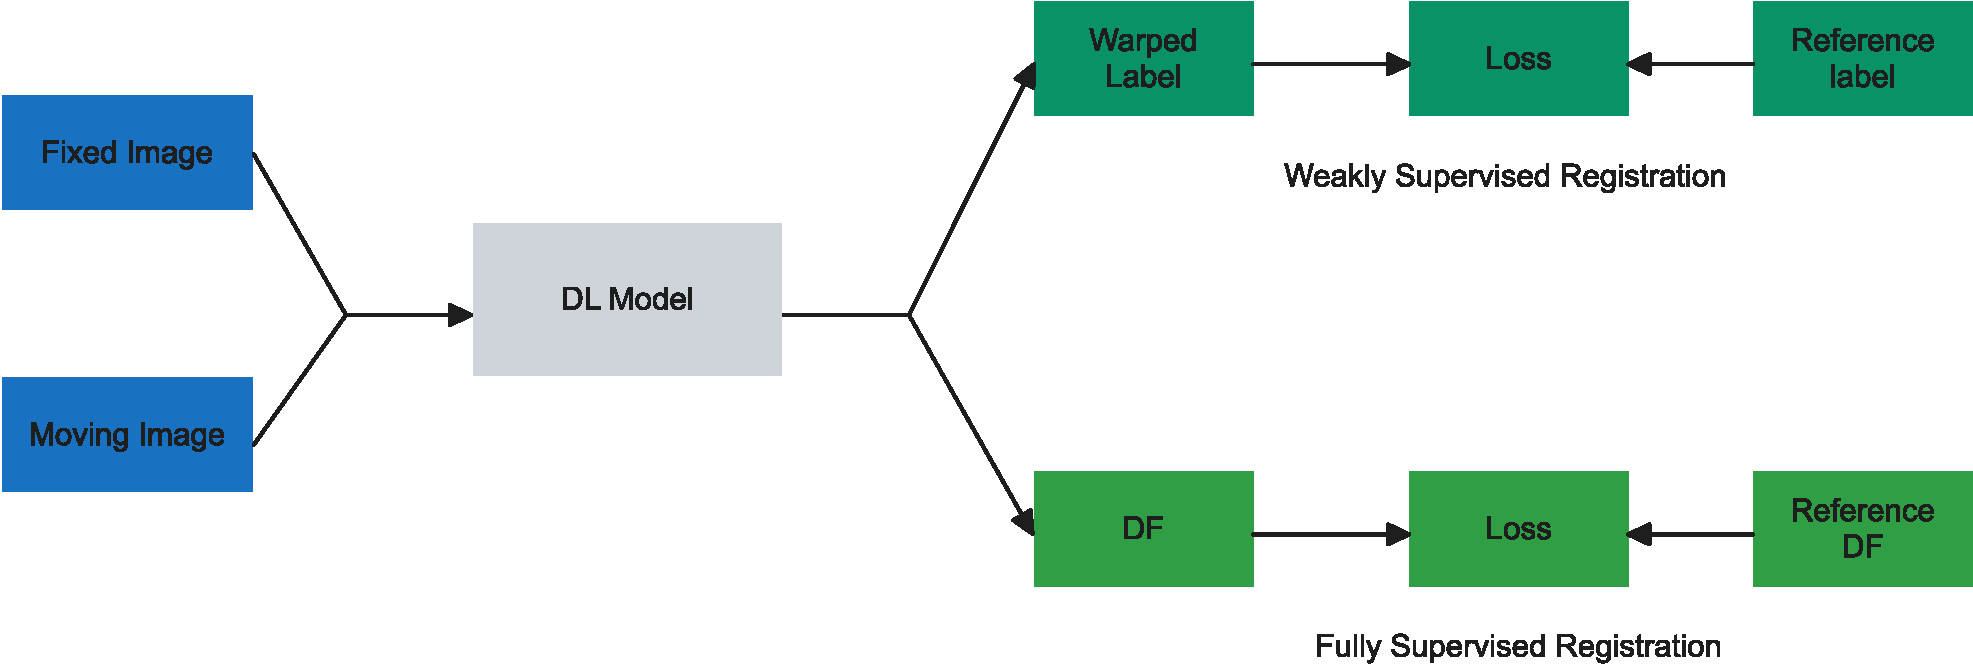
\includegraphics[width=0.9\textwidth]{fig1-Supervised Registration-crop.pdf}
    \caption{有监督配准模型}
    \label{fig:1}
\end{figure}

Miao等人首次采用深度学习算法预测图像的配准变换参数。他们指出现有的配准方法在计算速度和变形范围方面存在局限性,因此他们构建了一个五层的卷积神经网络(CNN)结构,利用CNN回归器直接估计变换参数,从而实现3D CT图像与2D X射线脊柱图像的刚性配准。相较于一些传统的基于强度的配准方法,该方法显著改善了配准效果\cite{miao2016cnn}。在后续研究中\cite{miao2016real},Miao等人提出了一种新的六层CNN网络结构,能够直接基于数字重建射线照片(DRR)和X射线图像来估计变换参数。该方法可以用较少的DRR渲染实现精准的2D/3D配准,且计算效率较高,更适合于实时应用。

Cao等人\cite{cao2018deep}使用了具有3个神经元的基于CNN的模型的输出层,其中每个神经元表示微小斑块中间沿x、y和z轴的运动幅度,能够得到与更传统的方法一样准确的结果。

Yang等人使用基于CNN的U-Net模型学习了具有相同分辨率的大脑MR图像的形变场,并在各种数据集上获得了出色的配准精度\cite{yang2017quicksilver}。

Uzunova等人采用了Flow Net框架\cite{dosovitskiy2015flownet},并使用三种方法生成标准标签数据\cite{uzunova2017training}:仿随机生成、仿射配准生成和统计外观模型(SAM)生成变换。然后,他们利用合成形变场对脑部和心脏的2D MR图像进行了配准。研究表明,在这三种方法中,使用基于SAM生成的标准标签数据进行CNN的学习和训练取得了最优效果。

Fan等人将监督损失与无监督损失相结合,利用双重监督来预测脑部3D MR配准的形变场。他们提出了一个分层双监督的全卷积网络(FCN)\cite{long2015fully}来解决缺少标准标签数据的问题\cite{fan2019birnet},该网络同时使用标准标签数据和图像相似性度量作为两种监督方式。网络的每一层都加入了损失函数,从而使一些层更容易收敛。基于U-net框架\cite{ronneberger2015u},Fan等人引入了间隙填充,提出了名为“BIRNet”的网络架构,该架构使用预测变换与标准标签数据之间的均方误差(MSE)作为损失函数,并结合预先配准的标准标签数据与图像相似性来训练网络。

Cao等人则采用了MR-MR损失和CT-CT损失两种损失进行双重监督配准\cite{cao2018deep},即在同模态内使用图像相似性来进行监督配准。他们在测试阶段直接根据输入的CT和MR图像预测变换场,通过预对齐图像将多模态配准转化为单模态配准,以实现MR-CT配准。此外,他们使用标准标签数据与预测变换扭曲的待配准图像之间的归一化互相关(NCC)作为损失函数。类似地,Liu等人也采用了监督合成变换和无监督图像相似性描述进行训练\cite{liu2019multimodal}。

\subsection{无监督图像配准}

相较于监督学习,基于无监督学习的配准方法就是在训 练学习网络时,只需要提供配准对,不需要标准标签数据(即真实的形变场)。因此,该类方法在训练与测试阶段,均不需要依靠传统的配准方法进行辅助。无监 督配准方法的流程如图\ref{fig:7}。

\begin{figure}[h]
    \centering
    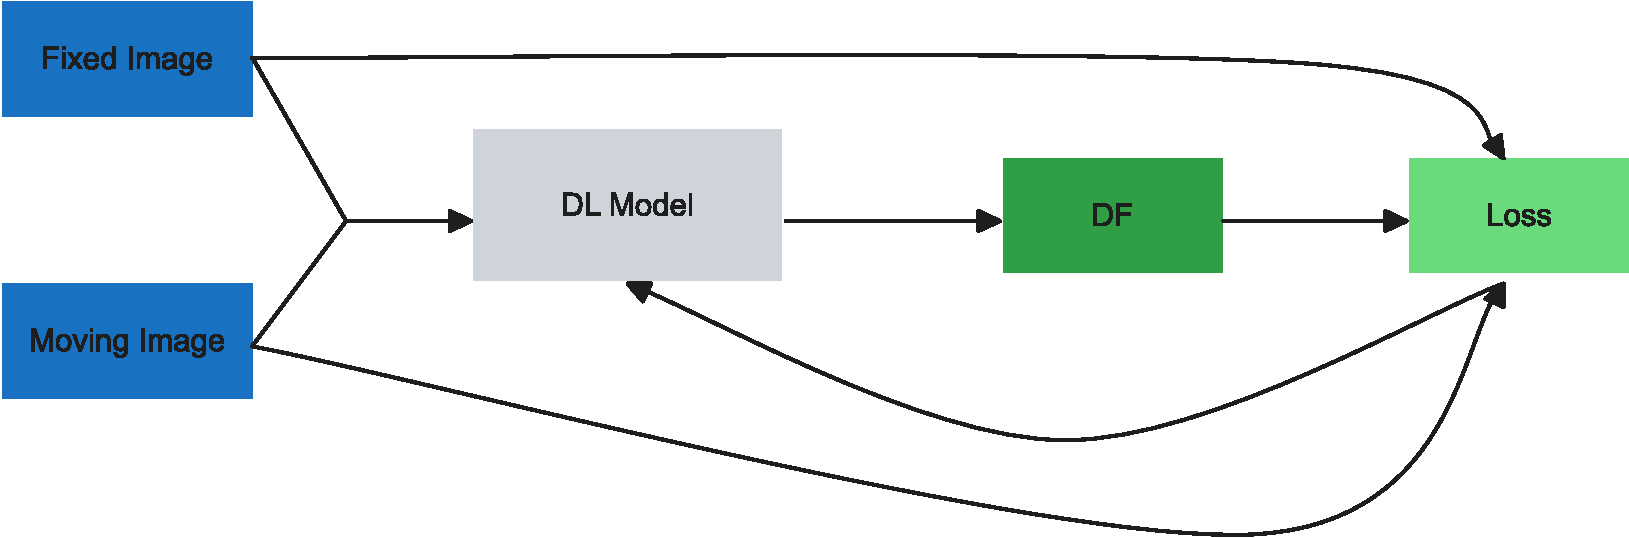
\includegraphics[width=0.9\textwidth]{fig7-unsupervised Registration-crop.pdf}
    \caption{无监督配准模型}
    \label{fig:7}
\end{figure}

de Vos等人提出了一个无监督的图像配准框架DLIR\cite{de2019deep},该框架利用固定图像和移动图像之间的相似性来训练网络,通过优化神经网络间接优化变换参数,预测的变换参数用于构建密集位移矢量场。在另一项研究中,de Vos等人提出了一种深度学习网络“DIRNet”\cite{de2017end},用于可变形图像配准。DIRNet由卷积神经网络回归器、空间变换器和重采样器组成,通过直接优化固定图像和移动图像之间的相似性来学习配准,从而实现心脏MR图像的配准。

Li等人同样利用图像相似性进行配准,通过最大化固定图像和移动图像之间的相似度直接估计图像对之间的空间变换。他们对全卷积网络(FCN)\cite{long2015fully}架构进行了改造,并采用多分辨率策略,以优化和学习在不同分辨率下的空间变化,同时将固定图像与移动图像之间的归一化互相关(NCC)及其他正则项作为损失函数。

相似地,Yoo等人\cite{avants2008symmetric}将卷积自动编码器(CAE)与空间变换网络(STN)\cite{jaderberg2015spatial}相结合,通过计算特征间的相似性,利用CAE以无监督的方式训练网络,实现对神经组织电子显微镜(ssEM)图像的无监督变换估计。

Balakrishnan等人设计了VoxelMorph配准框架\cite{balakrishnan2018unsupervised,balakrishnan2019voxelmorph},该框架由一个配准网络和一个分割网络组成,并在U-Net\cite{ronneberger2015u}的基础上进行了改造。该框架的损失函数结合了图像相似性与分割值的重合度,分割结果在一定程度上提高了配准的准确性。在后续的研究中,Dalca等人利用微分同胚来预测形变场,将均方误差(MSE)作为相似性度量,并与正则项结合构造损失函数,以实现脑部MR图像的无监督配准。

Alexander Bigalke等人提出了一种创新的配准网络RegCST\cite{bigalke2023unsupervised},该方法采用循环自训练策略进行递归训练。这一方法的核心在于其能够通过自我迭代地优化模型,使学习任务特定的特征更加鲁棒,尤其是在处理含噪声数据时。RegCST通过不断地更新和调整特征提取过程,极大地提高了所提取特征的表现力,使得配准结果在各类复杂场景下也能表现出色。此外,该网络在不同的医学成像数据集上进行了验证,展现出了优越的性能和广泛的适用性。

Wang等人提出了一种新颖的无监督配准网络PAN\cite{wang2024pyramid},该网络引入了自注意力机制和金字塔方法,以提高图像配准的效果。具体而言,PAN使用LAT模块,通过多尺度的形变场生成,来精准捕捉不同层次的特征信息。自注意力机制的引入使得模型能够集中关注图像中的关键信息,从而提升整体的配准质量。该网络不仅在保持高效性方面做出了重要贡献,同时也在多项实验中证明了其在各种图像配准任务中的优越性,包括处理高噪声和非刚性变形的数据。

Liu等人则提出了一种全新的无监督医学图像配准互学习范式MutualReg\cite{liu2024mutualreg}。该方法通过引入知识蒸馏机制,将教师网络和学生网络进行循环迭代更新,直到模型收敛为止。以教师网络为指导,学生网络不断吸收和重构知识,从而提高了配准性能。这种互学习的策略在多个医学图像数据集上验证了其有效性,取得了最佳的配准精度,尤其在处理多模态和多样本数据时表现尤为突出。MutualReg不仅优化了模型的学习过程,同时也推动了无监督配准技术的发展,为临床应用提供了更为精确和可靠的工具。


\section{主要研究内容及论文章节安排}

本文一共有七章,其中每章的安排如下:

第一章:绪论。首先介绍了基于金字塔结构与迭代优化的脑部医学图像配准的研究背景及意义;其次,介绍了医学图像配准的国内外研究现状;最后,介绍了本文的主要研究内容和章节安排。

第二章:训练与验证数据集介绍与选用。首先,介绍了用于脑部配准的MRI数据集及各自特点;其次,介绍了用于神经网络训练过程的数据集选用及预处理过程;再次,介绍了用于验证神经网络性能的数据集选用与预处理过程;最后,介绍了医学图像配准常用的评估,如定性评估和定量评估。

第三章:基于PAN网络的改进与预训练。首先,介绍了基于金字塔结构与自注意力机制的PAN网络的总体框架;然后,介绍了将PAN网络与训练数据集相适配的逻辑及实现;再次,介绍了对于PAN网络训练过程中损失函数的设计与改进;最后,通过与原始网络在验证数据集上的配准对比实验验证了PAN网络预训练阶段的性能与改进方法的有效性。

第四章:基于RegCST网络的改进与预训练。首先,介绍了基于CNN和迭代优化的RegCST网络的总体框架;然后,介绍了将RegCST网络与训练数据集适配的逻辑及实现;其次,介绍了RegCST网络在训练过程中的损失函数设计及改进方法;最后,通过在验证数据集上与原始网络的配准对比实验验证了改进方法的有效性与预训练阶段RegCST网络的性能。

第五章:基于MutualReg互学习配准框架设计。首先,介绍了基于互学习的MutualReg框架;其次,介绍了将本文两个模型与MutualReg框架相结合的逻辑与实现。

第六章:VRC模块消融分析。首先,介绍了对于VRC模块消融实验的目的;然后,介绍了VRC模块消融实验的设计;最后,通过在验证数据集上的配准对比实验验证VRC模块对于提升互学习配准性能的有效性。

第七章:互学习优化。首先,介绍了基于MutualReg的互学习优化实验设计;然后,通过不同互学习阶段网络在验证数据集上的配准对比实验验证了互学习对于提升配准性能的有效性。

\chapter{训练与验证数据集介绍与选用}

\section{训练数据集选用}

在预训练和递归互学习阶段,采用Learn2Reg(L2R)挑战赛的大规模无监督脑部MRI图像配准(LUMIR)数据集进行训练,训练数据集中包含3384张图像。其核心特点是仅提供大量的无标注原始图像,不限制具体的图像配对方式,由参与者自由创建图像对,为深入的无监督学习提供了高度的灵活性。因此,在使用LUMIR数据集进行训练之前需要根据其图像数据创建训练图像对。

为了充分利用大规模数据集的数据量优势,并且防止过多质量较差数据对于模型性能以及训练过程中收敛困难的问题,在预训练阶段,采用基于均方误差(MSE)的相似性指标建立训练图像对。具体而言,图像对建立过程如下:

\begin{enumerate}
    \item 对于每两对图像,计算其MSE指标作为这两张图像的相似度指标
    \item 依次选择相似度最高的两张图像进行配对
    \item 直到每张图像都有与之配对的图像
    \item 对每对图像进行快速仿射对齐
\end{enumerate}

同时,为了避免过多低质量或无意义的图像对参与训练,并且提高配对数据的整体质量,每张图像被限制最多与2张图像进行配对。经过筛选后,总共得到了1835对训练图像。这一策略通过优先选择解剖结构对齐程度较高的图像对,降低了初始训练的优化复杂度,同时通过配对数量限制避免模型过度依赖局部相似模式,为后续无监督学习提供了稳定且多样化的数据基础。

这样做有以下的优势

\begin{itemize}
    \item \textbf{减低训练初期的优化难度}:高相似度图像对之间的形变场相对于低相似度图像对之间的形变场通常复杂度较小,可为模型提供更为平滑的优化目标,避免梯度方向剧烈波动导致初期训练难度增加导致模型收敛困难。
    \item \textbf{隐式数据增强}:严格限制图像之间的一一配对可能限制训练样本的多样性,为此将每张图像的配对数量放宽至2,增加训练数据的多样性;并且也能够控制训练图像对数,防止训练时间过长。
    \item \textbf{降低模型收敛困难的风险}:通过相似性筛选,能够保证训练样本的相似度,防止随机配对导致部分相似度低的图像参与训练影响模型性能以及出现收敛困难的风险。
\end{itemize}

\section{验证数据集选用}

LUMIR测试集包含590张脑部MRI图像,但缺乏分割标签与解剖标记点信息,可以用来测试最终模型产生位移场的平滑度指标,但是无法用于评价配准精度的Dice指标的测试。为此,选用同样为脑部MRI配准任务的LPBA40数据集作为课题的验证数据集。LPBA40数据集包含40例健康受试者的3D脑MRI扫描数据,每例数据均附带56个脑区的手动精细标注,涵盖海马体、丘脑等关键解剖结构,能够用于Dice指标的测试。

为了保证评价的严谨性,在LPBA40数据集测预处理过程中,对其中的图像进行N4偏置场校正与Z-Score强度归一化。同时对训练数据也做同样的处理,避免因为两个数据集强度分布不一致对最终评价结果产生影响。

此外,测试阶段采用双重验证机制:首先通过可视化叠加展示配准前后的解剖结构对齐效果,定性评估形变场的合理性;随后基于Dice系数和平滑性指标定量分析模型性能。该预处理框架通过数据标准化与空间对齐,在兼顾数据质量与多样性的同时,充分利用了大规模无监督数据的潜力。LUMIR数据集在预训练阶段提供了稳定且丰富的形变模式,LPBA40数据集则为精确的配准精度评估提供了坚实基础。双重验证机制既能定性展示模型在解剖结构对齐上的效果,又可通过多指标(Dice、平滑度)定量分析模型的优缺点,从而为后续的模型迭代与改进提供全面、可靠的依据。

\section{医学图像配准的评估}

医学图像配准的评估分为两种:定性评估和定量评估。其中定性评估容易受主观影响,因此在评判中一般以定量评估为主,定性评估作为辅助。

\subsection{定性评估}

定性评估主要分为两种:可视化评估和差分图像评估。

\paragraph{可视化评估}

可视化评估主要依靠肉眼观察对配准后图像与固定图像的相似性进行评估。如图\ref{fig:c2-1}、\ref{fig:c2-2}、\ref{fig:c2-3},可以看出,经过配准过后得到的配准图像与固定图像更为相似,因此认为该配准效果较好。

\begin{figure}[h]
    \centering
    \begin{minipage}{0.3\textwidth}
        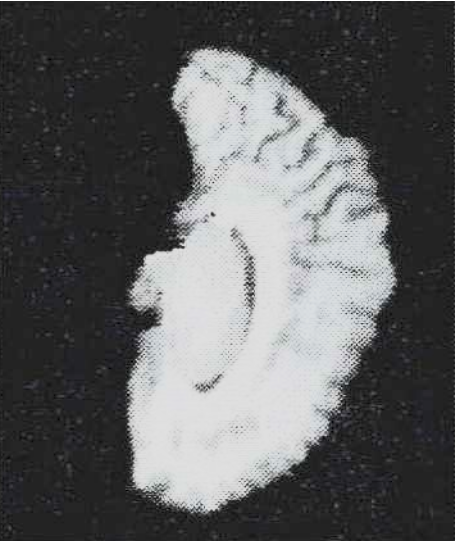
\includegraphics[width=\textwidth]{c2-fiximg.png}
        \caption{固定图像}
        \label{fig:c2-1}
    \end{minipage}
    \begin{minipage}{0.3\textwidth}
        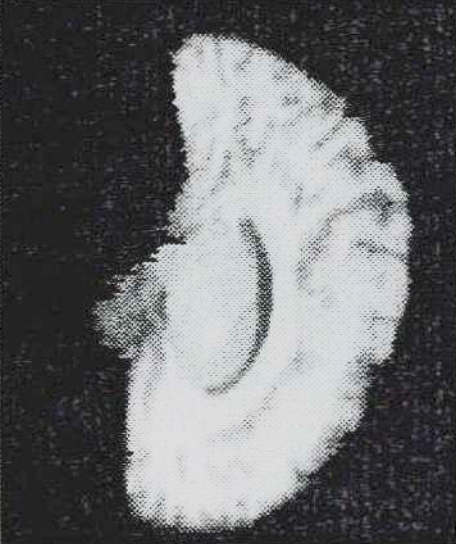
\includegraphics[width=\textwidth]{c2-moveimg.png}
        \caption{浮动图像}
        \label{fig:c2-2}
    \end{minipage}
    \begin{minipage}{0.3\textwidth}
        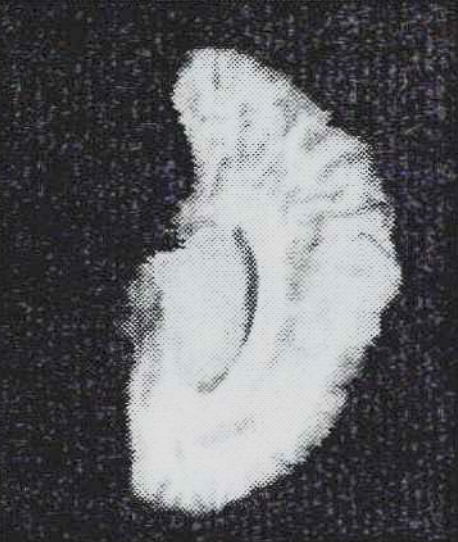
\includegraphics[width=\textwidth]{c2-regimg.png}
        \caption{配准图像}
        \label{fig:c2-3}
    \end{minipage}
\end{figure}

在有分割标签时,可将配准后的标签叠加在固定图像上以便于更好的观察两幅图像特定解剖结构的相似性,如图\ref{fig:c2-4}。

\begin{figure}[h]
    \centering
    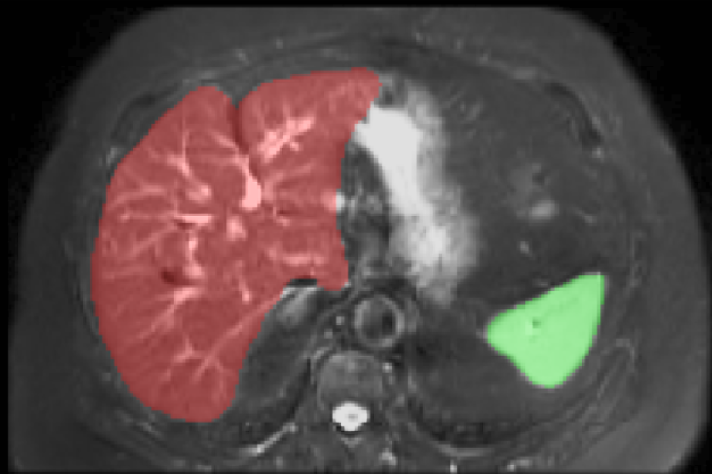
\includegraphics[width=0.9\textwidth]{c2-markedimg.png}
    \caption{带分割标签的可视化图像}
    \label{fig:c2-4}
\end{figure}

\paragraph{差分图像评估}

相较于肉眼观察,差分图的方式更为直观。将配准图像与固定图像做差分即可得到差分图,差分图越接近黑色,表示配准效果越好,反之效果越差。

\begin{figure}[h]
    \centering
    \begin{minipage}{0.4\textwidth}
        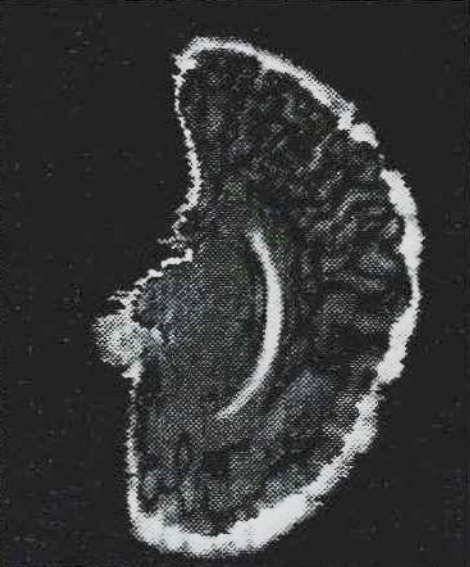
\includegraphics[width=\textwidth]{c2-imgdiff1.png}
        \caption{浮动图像差分图}
        \label{fig:c2-5}
    \end{minipage}
    \begin{minipage}{0.4\textwidth}
        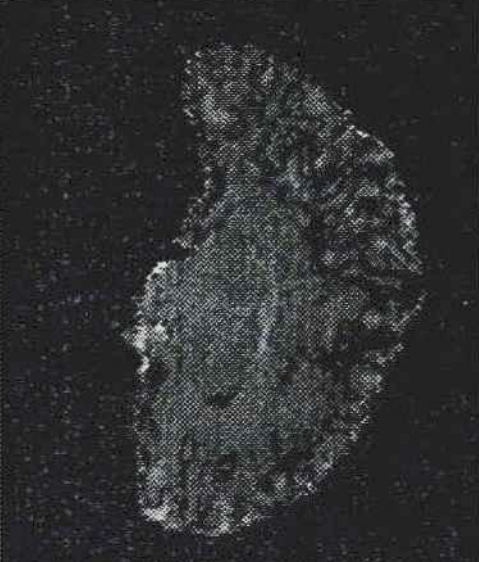
\includegraphics[width=\textwidth]{c2-imgdiff2.png}
        \caption{配准后图像差分图}
        \label{fig:c2-6}
    \end{minipage}
\end{figure}

图\ref{fig:c2-5}是浮动图像与固定图像的差分图,可以看出在大脑边缘两张图像并不对齐,有较多的白色区域,表明固定图像与浮动图像在该区域相似性不佳。图\ref{fig:c2-6}是经过配准后的配准图像与固定图像的差分图,图像基本呈现黑色,尤其在边缘部分,表明配准后图像已经基本对齐。

\subsection{定量评估}

定量评估主要分为两类:评价配准精度的指标如Dice系数;评价形变场平滑度的指标如雅可比行列式、SDlogJ。

\paragraph{Dice系数}

Dice系数主要用于评估固定图像与配准后图像在对应解剖区域的重叠程度,Dice系数的计算如公式\ref{eq:c2-1}。

\begin{equation}
    \mathrm{Dice}(A,B)=2\times\frac{\left|A\cap B\right|}{\left|A\right|+\left|B\right|}
    \label{eq:c2-1}
\end{equation}

其中$A$和$B$分别表示固定图像与配准后图像相对应的解剖区域,Dice系数越接近1,代表配准后在对应解剖区域的相似性越高,配准精度越高,反之配准精度越低。

\paragraph{雅可比行列式}

雅可比行列式常用于评价形变场的平滑性。以三维数据为例,在形变场上的每个点的雅可比行列式计算如公式\ref{eq:c2-2}:

\begin{equation}
    \centering
    \det(J(i,j,k))=\begin{vmatrix}\frac{\partial i}{\partial x} & \frac{\partial j}{\partial x} & \frac{\partial k}{\partial x} \\\frac{\partial i}{\partial y} & \frac{\partial j}{\partial y} & \frac{\partial k}{\partial y} \\\frac{\partial i}{\partial z} & \frac{\partial j}{\partial z} & \frac{\partial k}{\partial z}\end{vmatrix}
    \label{eq:c2-2}
\end{equation}

\paragraph{SDlogJ}
SDlogJ(Standard Deviation of Logarithmic Jacobian determinant)用于量化形变场局部体积变化的离散程度。其计算基于雅可比行列式,具体过程如公式\ref{eq:sdlogj}所示:

\begin{equation}
    \centering
    \text{SDlogJ} = \sqrt{ \frac{1}{N} \sum_{(x,y,z) \in \Omega} \left( \log \det(J(x,y,z)) - \mu_{\log J} \right)^2 }
    \label{eq:sdlogj}
\end{equation}

其中:
\begin{itemize}
    \item $\det(J(x,y,z))$为点$(x,y,z)$的雅可比行列式,计算方法如公式\ref{eq:c2-2}所示
    \item $\mu_{\log J} = \frac{1}{N} \sum_{(x,y,z) \in \Omega} \log \det(J(x,y,z))$为有效区域内对数雅可比行列式的均值
    \item $N$为满足$\det(J) > 0$的体素总数,排除$\det(J) \leq 0$的折叠区域
\end{itemize}

该指标通过标准差度量$\log \det(J)$的离散度,对异常体积变化具有更高敏感性。SDlogJ趋近于零时表明形变场具有均匀的体积变化特性,较大值则提示局部存在剧烈膨胀或收缩。

\section{本章小结}

本章阐述了医学图像配准研究中训练与验证数据集的构建策略及评估方法体系。针对无监督学习框架对大规模数据的需求,选用LUMIR挑战赛的3384张脑部MRI图像作为训练数据源,通过基于均方误差的相似性筛选机制构建1835对高质量训练样本。为克服LUMIR测试集缺乏标注的局限性,引入LPBA40数据集作为验证基准,其40例含56个脑区精细标注的MRI数据,为定量评估提供了可靠的解剖对齐参照。

在数据预处理环节,采用N4偏置场校正与Z-Score强度归一化的标准化流程,确保训练与验证数据的强度分布一致性,消除跨数据集偏差对评估结果的干扰。

在评估方法层面,介绍了定性分析与定量指标的多维度评价体系。定性评估通过配准图像与固定图像的叠加可视化、解剖标记融合显示以及差分图分析,直观呈现形变场的空间合理性;定量评估则基于Dice系数衡量关键解剖结构的重叠精度,结合雅可比行列式及其对数标准差(SDlogJ)量化形变场的拓扑保持能力与局部平滑特性。


\chapter{基于 MutualReg 互学习配准框架设计}

\section{MutualReg互学习配准框架介绍}

MutualReg的核心理念是,任何网络都可以通过互学习(ML)从自身的无监督损失和另一个网络的有监督损失中进行递归学习。其有监督损失是通过知识蒸馏(KD)机制实现的。MutualReg的目标是通过互学习整合多种损失信息,如图\ref{fig:2}。此外,采用VRC模块以确保仅保留知识蒸馏中可靠的体素位置。

\begin{figure}[h]
    \centering
    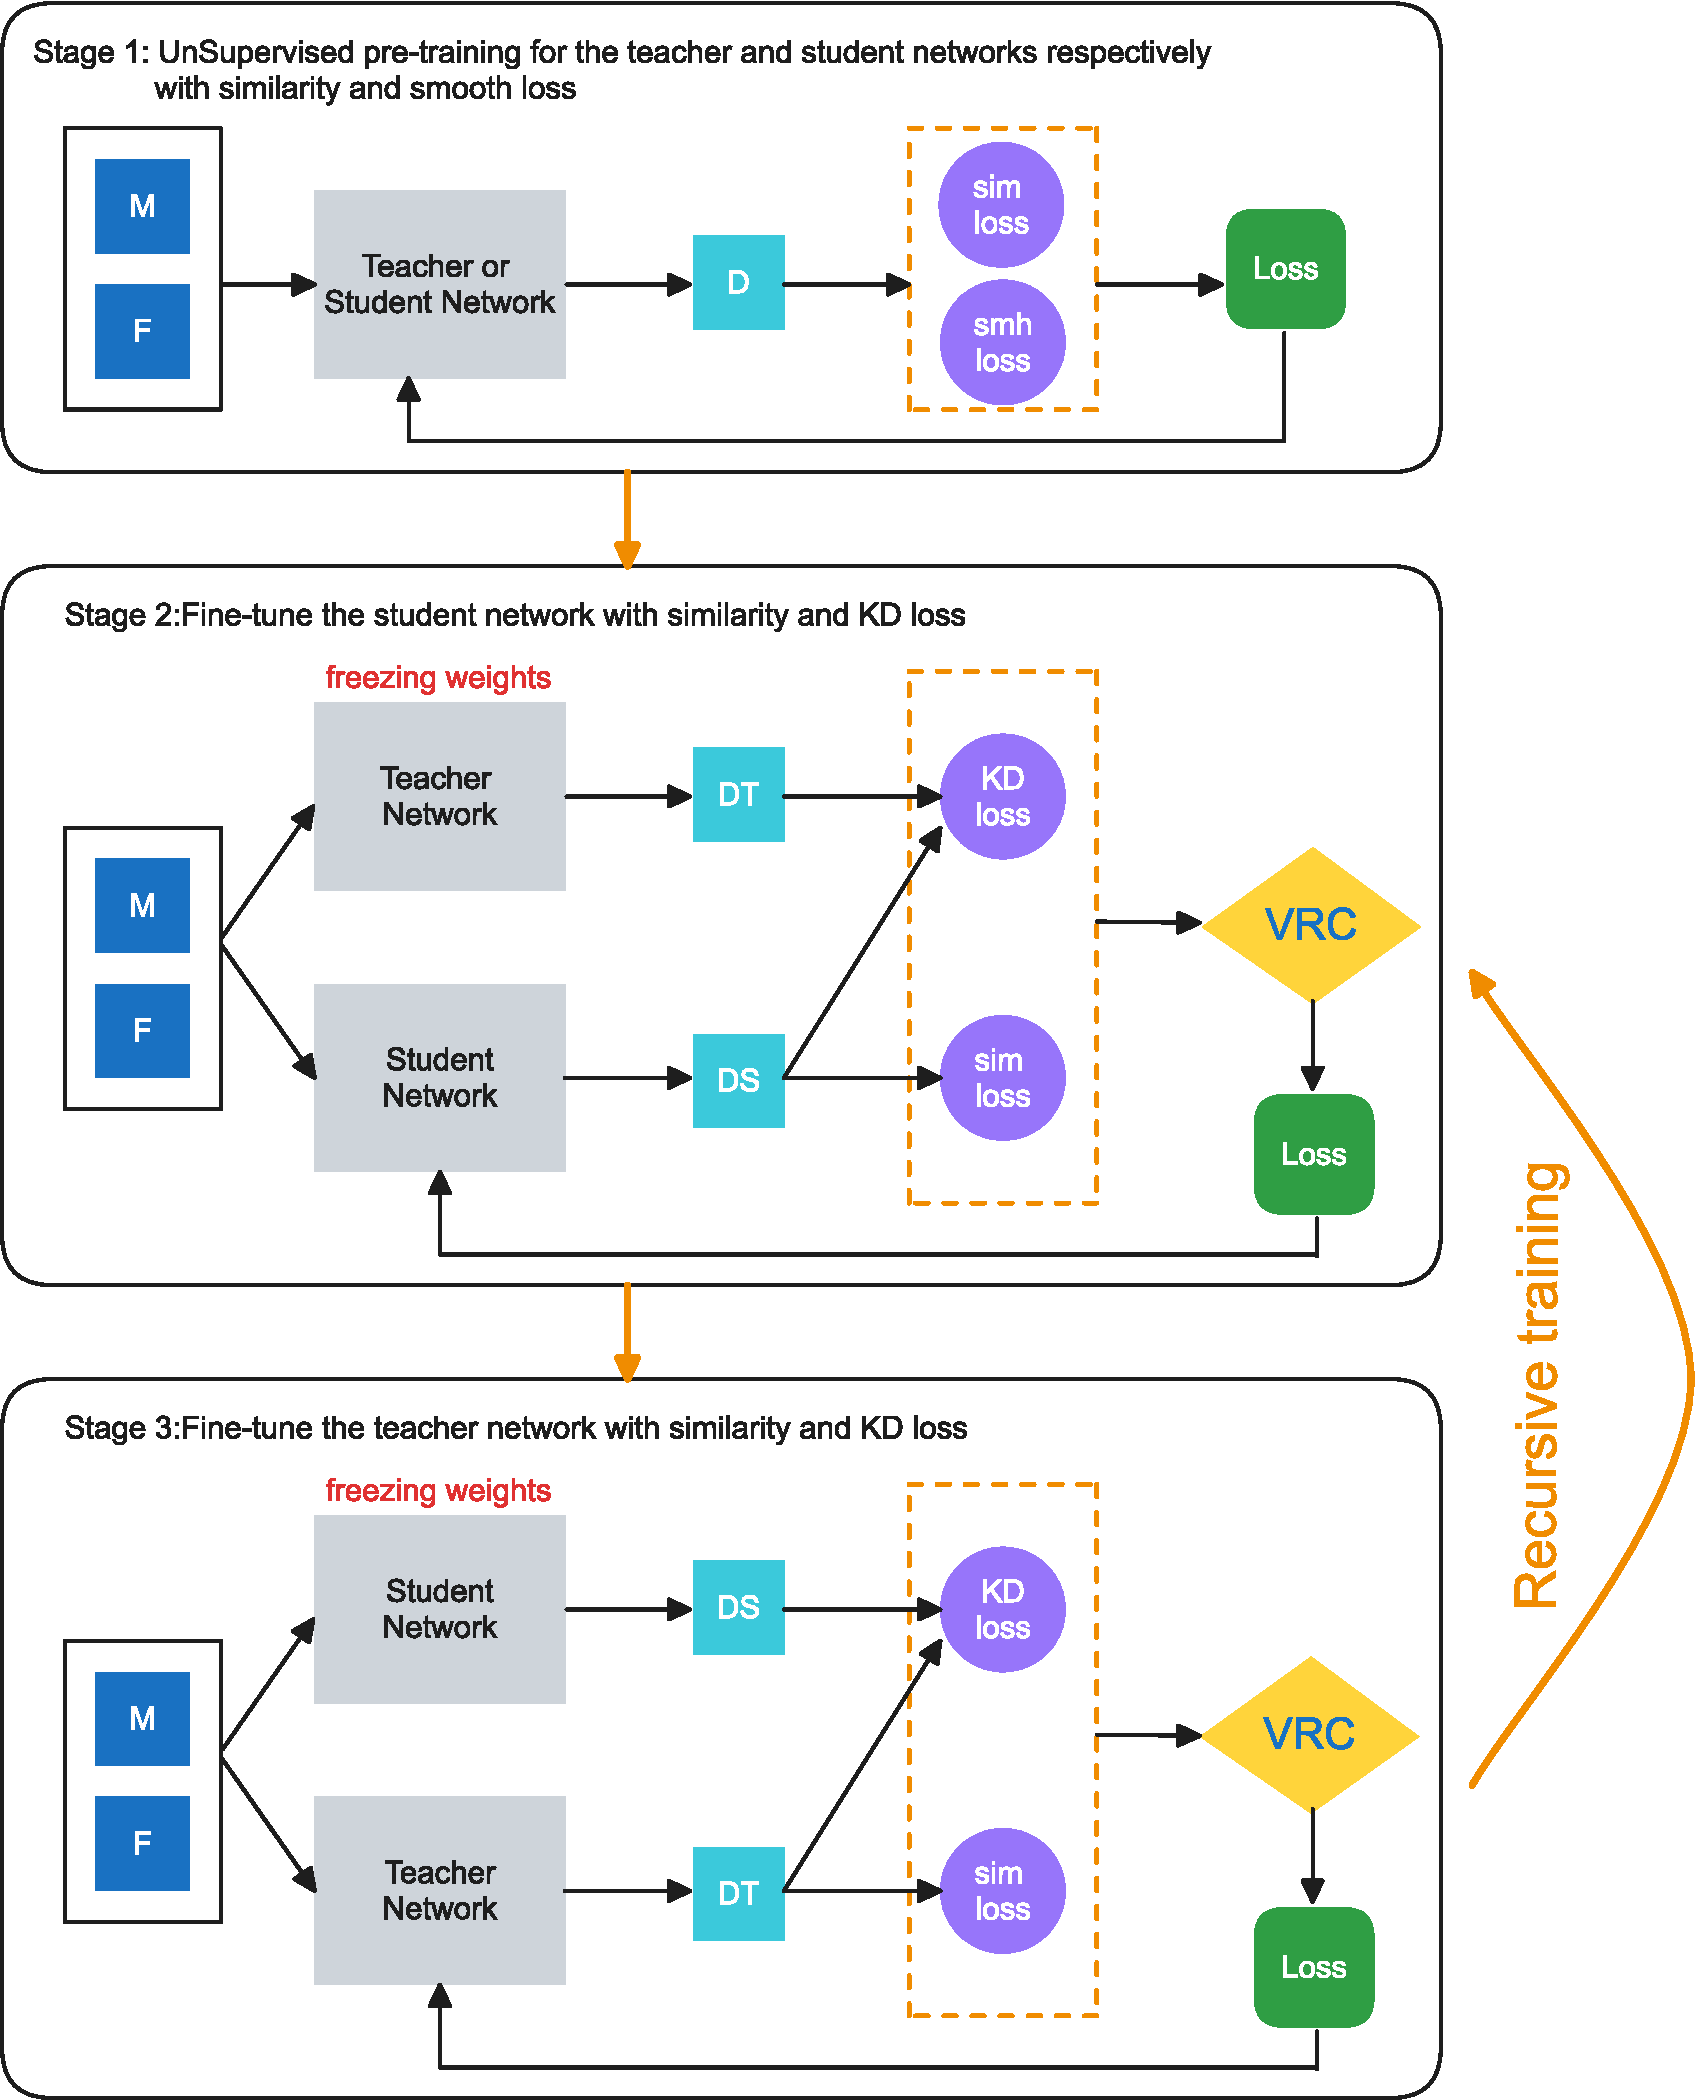
\includegraphics[width=0.9\textwidth]{fig2-mutualreg-crop.pdf}
    \caption{MutualReg的详细框架}
    \label{fig:2}
\end{figure}

具体而言,MutualReg的训练过程为:

\begin{enumerate}
    \item 在第一阶段,使用常见的无监督学习方法对教师和学生网络进行预训练
    \item 学生和教师网络分别在第二和第三阶段通过相互学习进行微调
    \item 递归训练学生和教师网络,直到收敛
\end{enumerate}


\section{教师网络与学生网络选用与介绍}

\subsection{教师网络介绍}

PAN网络是一种用于医学图像配准的无监督深度学习方法,通过结合双流金字塔编码器和多头局部注意力Transformer解码器,有效解决了传统卷积神经网络特征增强不足及Transformer信息冗余的问题。编码器采用通道注意力机制增强多层次特征表示,解码器通过局部注意力Transformer分析运动模式并生成平滑变形场,同时引入正交正则化减少特征冗余以提升运动模式建模能力。其网络架构如图\ref{fig:4}。

\begin{figure}[h]
    \centering
    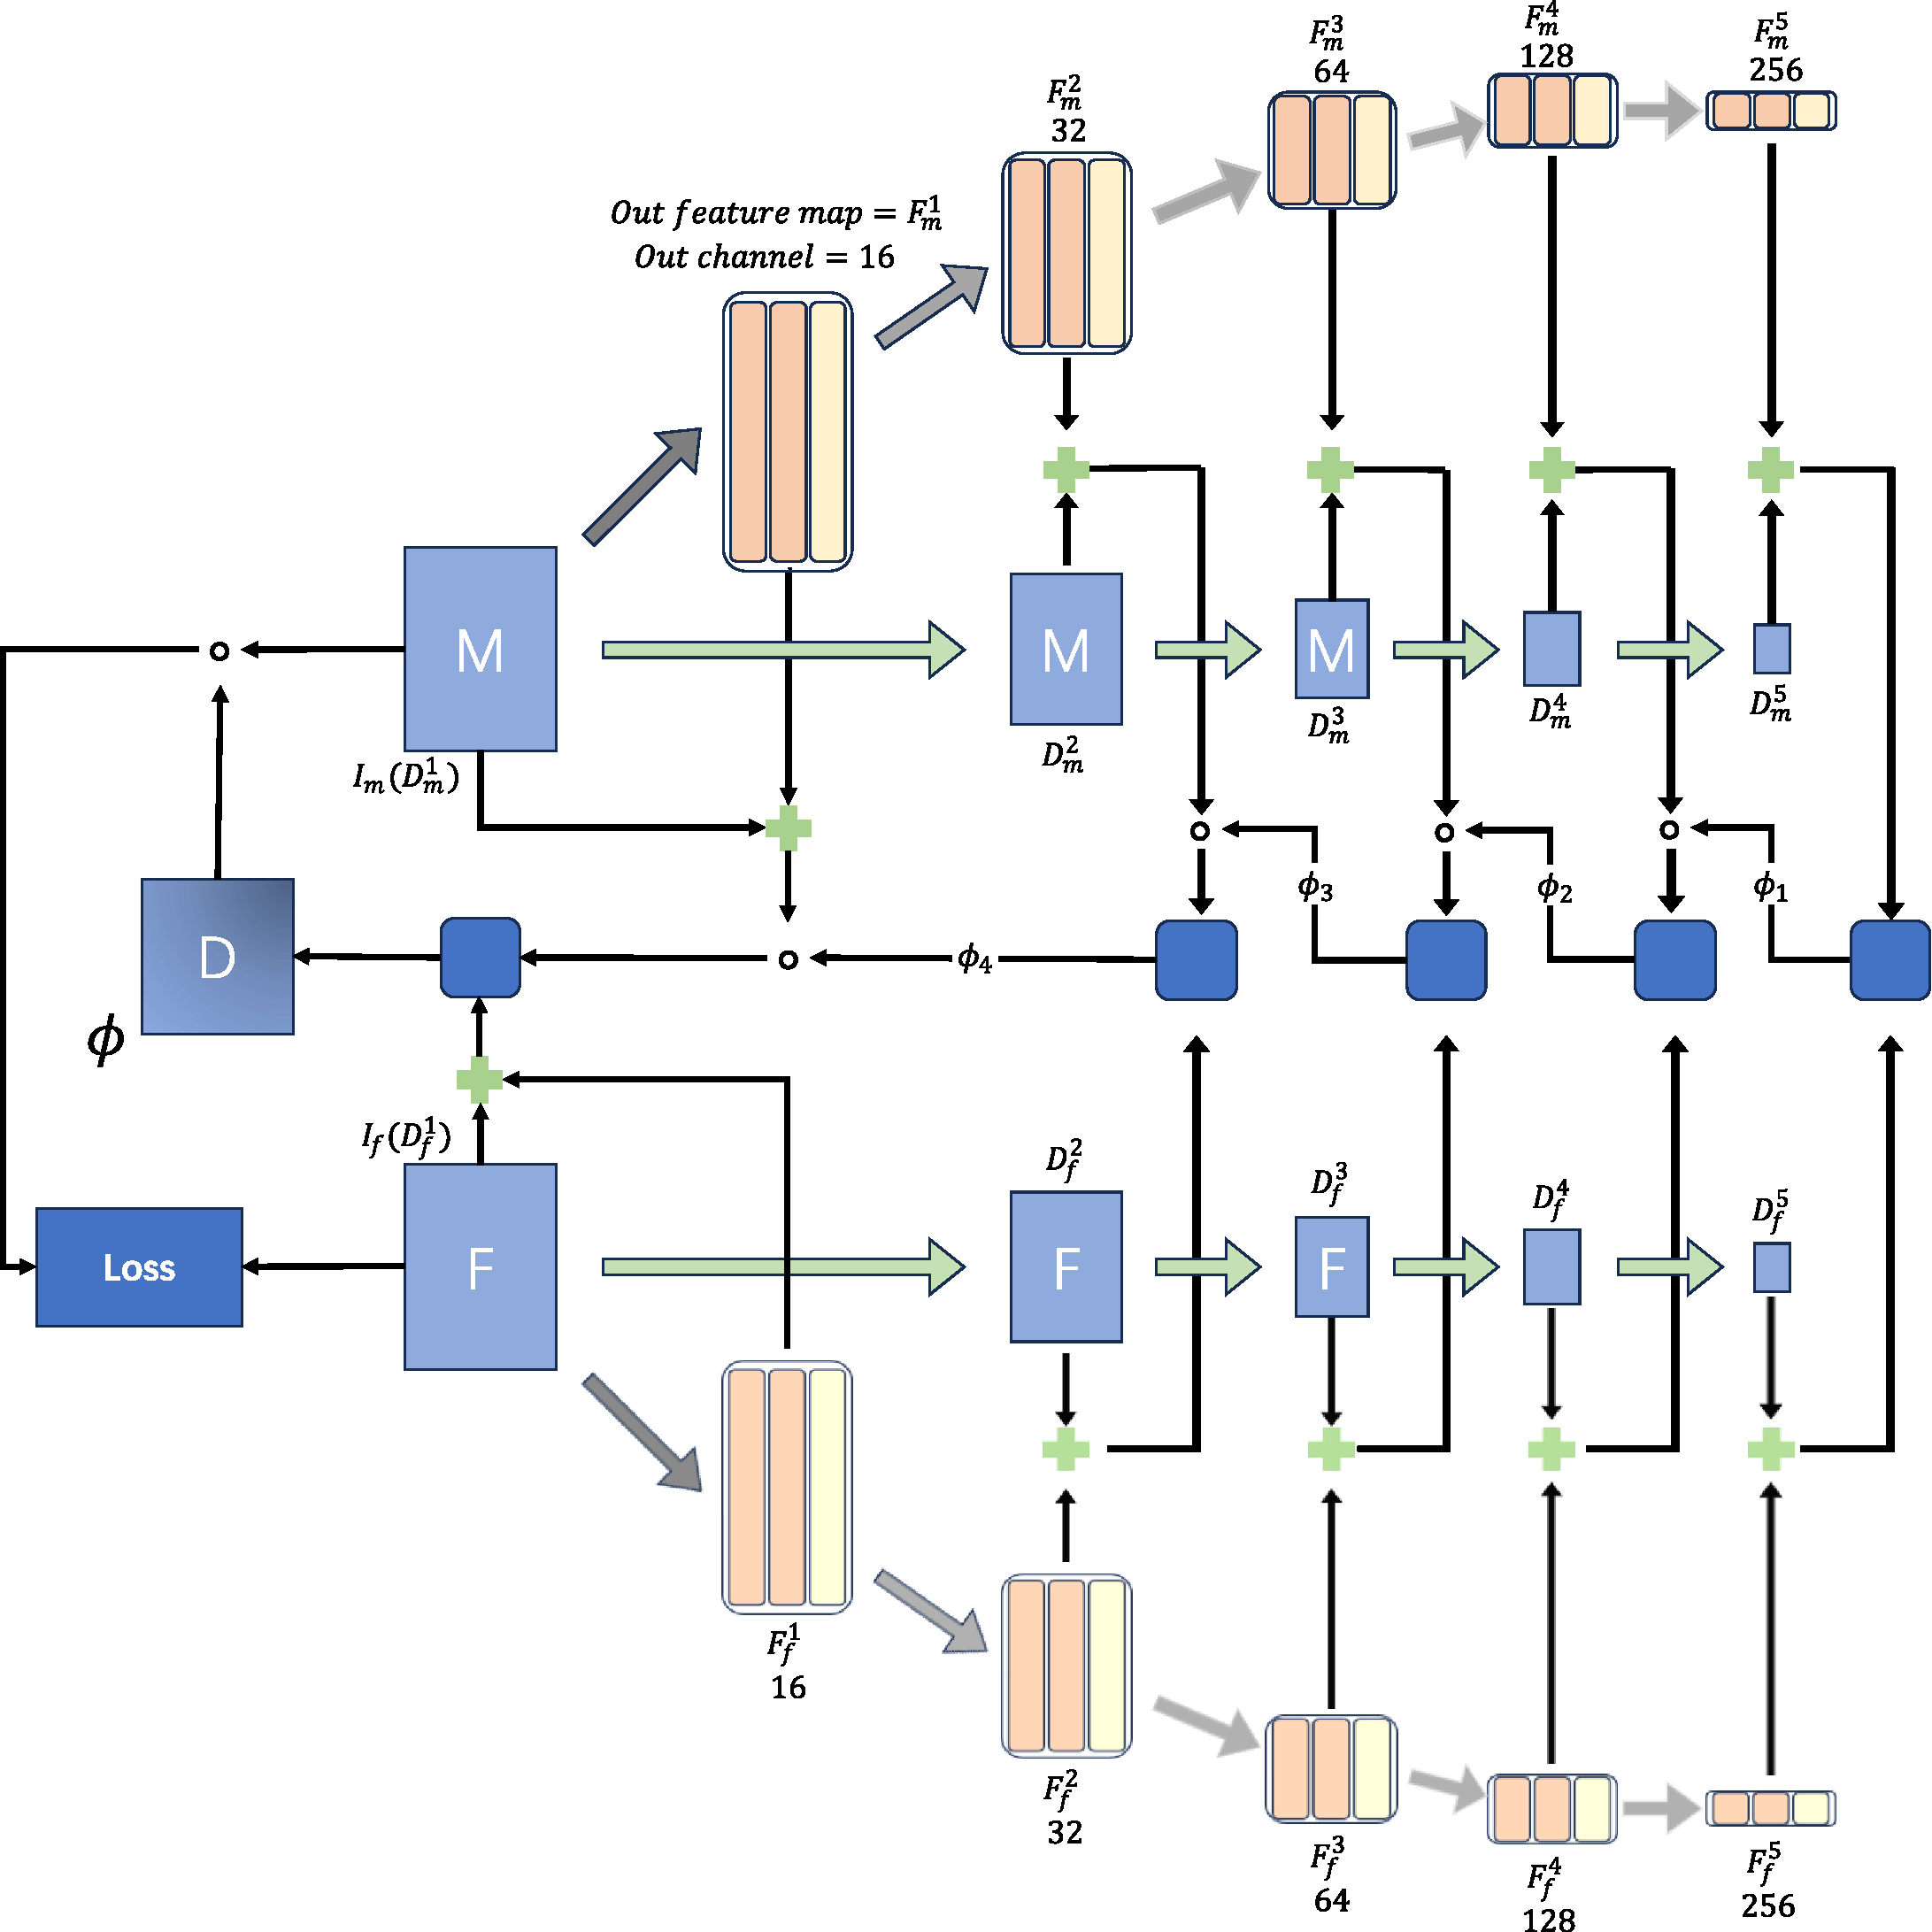
\includegraphics[width=0.9\textwidth]{fig4-PAN-crop.pdf}
    \caption{PAN网络架构}
    \label{fig:4}
\end{figure}

其网络主要由双流金字塔编码器和局部注意力Transformer解码器组成。

双流权重共享的金字塔编码器使用运动图像$I_m$和固定图像$I_f$作为输入,并通过一系列通道注意力块生成两组分组特征:$\{F_m^1,F_m^2,F_m^3,F_m^4,F_m^5\}$和$\{F_f^1,F_f^2,F_f^3,F_f^4,F_f^5\}$。同时,$I_m$和$I_f$经过下采样生成图像集$\{D_m^1,D_m^2,D_m^3,D_m^4,D_m^5\}$和$\{D_f^1,D_f^2,D_f^3,D_f^4,D_f^5\}$,并于相对对应的特征图进行对齐。

对于每个通道注意力块,使用两个卷积块(每个块都有一个$3\times3\times 3$的卷积层、一个实例归一化层\cite{ulyanov2016instance}和一个LeakyReLU激活层)和一个压缩和激励(SE)块\cite{hu2018squeeze}。SE块通过结合全局信息动态优化特征图,促进编码器生成更具代表性的特征。

在解码器部分,利用局部注意力Transformer(LAT),来解析特征图并推导出形变场。首先将$(F_m^5,D_m^5)$和$(F_f^5,D_f^5)$输入LAT模块,以分析形变并生成初始形变场$\phi_1$。之后利用$\phi_1$对$(F_m^4,D_m^4)$进行形变,并将$(F_m^4\circ \phi_1,D_m^4\circ\phi_1 )$和$(F_f^4,D_f^4)$做为后续LAT的输入,生成$\phi_2$。类似的,生成$\phi_3,\phi_4$和最终的形变场$\phi$。

作为教师网络,PAN网络不仅能引导学生网络识别和关注关键区域,还能通过其强大的特征选择能力,促进学生网络的学习。

\subsubsection{局部注意力Transformer模块}

局部注意力Transformer模块用于生成每个下采样层的形变场。具体而言将编码器特定层的运动图像特征图、固定图像特征图及其相应的降采样图像分别表示为 \( F_m \)、\( F_f \)、\( D_m \) 和 \( D_f \)。之后,将 \( (F_f, D_f) \) 和 \( (F_m, D_m) \) 在通道维度上进行连接。然后,连接后的特征通过线性投影(LP)和层归一化(LayerNorm,LN)计算查询(Q)和键(K),具体表达如下:

\begin{equation}
    Q = LN(LP(\text{concat}(F_f, D_f)))
\end{equation}

\begin{equation}
    K = LN(LP(\text{concat}(F_m, D_m)))
\end{equation}

对于多头注意力机制,\( Q \in \mathbb{R}^{S \times h \times w \times l \times \frac{c}{S}} \) 和 \( K \in \mathbb{R}^{S \times h \times w \times l \times \frac{c}{S}} \) 可以按注意力头的数量 \( S \) 划分为 \( \{ Q_1, Q_2, \ldots, Q_S \} \) 和 \( \{ K_1, K_2, \ldots, K_S \} \),其中 \( c \) 是通道数。那么,第 \( s \) 个注意头的局部注意力图 \( LA \) 可以通过以下公式计算:

\begin{equation}
    LA_s = \text{softmax}\left(Q_s \cdot K_s^T + P_s\right)
\end{equation}

其中 \( N(x) \) 表示体素 \( x \) 的 \( N \times N \times N \) 邻域,\( P \in \mathbb{R}^{S \times N \times N} \) 是可学习的相对位置偏差。

局部注意力图 \( LA \) 蕴含了不同运动模式的信息。因此,可以利用局部注意力图对规则形变场进行加权,以生成一系列可能的形变子场:

\begin{equation}
    \phi_s = LA_s \cdot V
\end{equation}

其中 \( V \in \mathbb{R}^{n \times n \times n} \) 表示邻域质心的相对位置坐标。

最后,通过卷积层合并来自每个注意头的形变子场 \( \{ \phi_1, \phi_2, \ldots, \phi_S \} \),以在第 \( t \) 个解码层生成最终的形变场 \( \phi_t \in \mathbb{R}^{h \times w \times l \times 3} \)。

在多头学习中会出现潜在同质性问题。潜在同质性可能导致信息冗余,使得多个头部学习到相似的特征,从而降低模型的区分能力和整体性能。这种同质化会导致特征表达不足,影响模型在多类别任务中的判别性,同时也使训练效率降低,浪费计算资源。

因此,为了解决多头LAT学习内容的潜在同质性,PAN网络在LAT模块中使用正交损失$L_{orth}$对特征学习进行正则化\cite{brock2016neural}。

首先将查询(Q)和键(K)根据注意力头的维度转换为平面向量,形成一个矩阵 \( W \in \mathbb{R}^{S \times u} \)(其中 \( u = h \cdot w \cdot l \cdot c_s \))。在获得矩阵 \( W \) 之后,对每个头部所表示的向量进行归一化处理,并与其转置相乘。最终,正交性损失 \( L_{\text{orth}} \) 可以通过以下公式计算:
\begin{equation}
    L_{\text{orth}} = L_{\text{MSE}}\left(\text{Norm}(W) \cdot \text{Norm}(W)^T, I\right)
\end{equation}

其中,\( I \) 是单位矩阵,\( L_{\text{MSE}} \) 是均方误差(即 \( l_2 \) 范数)的计算。

\subsection{学生网络介绍}

RegCST是一种基于循环自训练策略的无监督3D医学图像配准框架,其核心架构通过深度融合深度特征提取网络与可微分优化算法,实现了从伪标签生成到网络参数更新的闭环优化。如图\ref{fig:regcst}所示,该网络主要由特征提取模块、优化器模块及自训练机制三部分构成。特征提取模块采用标准3D卷积神经网络,包含6层卷积操作,每层卷积核尺寸为$3 \times 3 \times 3$,通道数逐层递增(32、64、128),并通过步长为2的下采样将输入图像分辨率缩减至原始尺寸的1/8。网络末端通过$1 \times 1 \times 1$卷积将固定图像与移动图像的特征映射至16维空间,并输入相关性层计算多尺度位移匹配响应,为后续优化提供高判别性特征表示。

\begin{figure}[h]
    \centering
    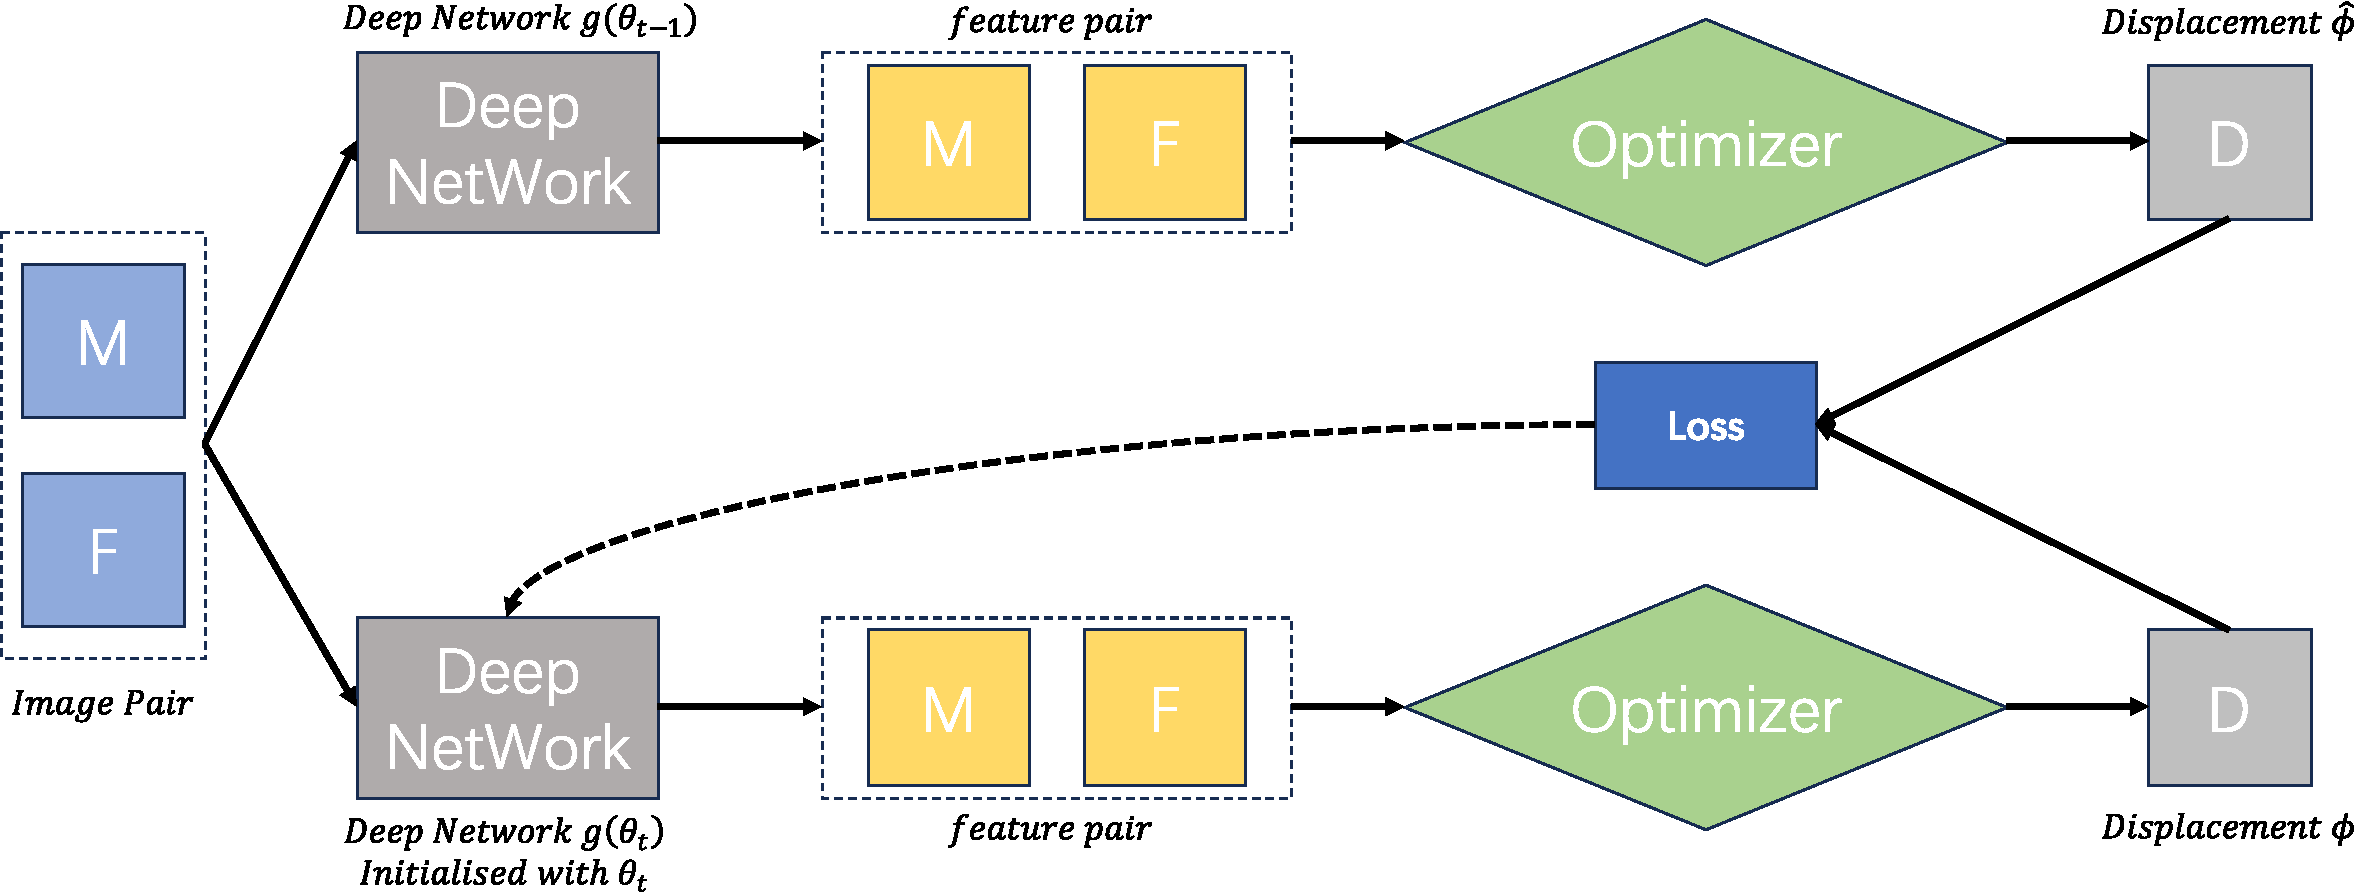
\includegraphics[width=0.9\textwidth]{fig5-cst-crop.pdf}
    \caption{Dice系数随训练epoch的变化曲线}
    \label{fig:regcst}
\end{figure}

对于优化器,采用耦合凸优化器\cite{siebert2022learn},其在给定固定图像和移动图像特征图的情况下,推断出一个位移场,该位移场最小化了平滑度和特征相异度的组合目标。其优化过程包含三个关键步骤:前向-后向一致性约束以减少位移场双向误差、基于变形图像的二次特征对齐以细化局部匹配,以及实例级Adam微调以联合优化特征相似性与正则化项。

\subsubsection{循环自训练策略}

RegCST的创新性主要体现在其循环自训练机制上。该机制摒弃了传统无监督方法对人工设计相似性度量的依赖,转而通过多阶段交替优化伪标签与网络参数实现自我增强。具体而言,网络初始化阶段利用随机权重特征提取网络生成初始伪位移场,随后通过目标配准误差(TRE)损失函数监督特征网络的训练。每一训练阶段结束后,利用当前网络生成更精确的伪标签,并通过学习率热重启策略跳出局部最优,进入下一轮迭代。针对腹部CT配准任务,该过程通常需经过8个阶段以收敛至最优性能。

RegCST网络采用随机初始参数$\theta_0$初始化特征提取网络来获得用于训练第一个特征提取网络的伪标签监督。

这种设置存在一个关键问题:网络可能会过度拟合初始伪标签,并学习再现的是随机特征。因此,受到对比学习\cite{chen2021exploring}的启发,RegCST网络通过在两个层面上将不对称性纳入学习和伪标签流来提高特征学习的效率。首先,对两个流中的输入对应用不同的随机增广。其次,在优化器之后通过额外微调和正则化步骤来增强伪标签流,以改善伪位移场包括以下三个部分:

\begin{itemize}
    \item 计算反向位移场,然后迭代地最小化两个场之间的差异;这种计算确保了无论数据是朝哪个方向(固定图像到移动图像或反向)进行处理,网络都能够保持一致性,从而提高了最终预测的准确性
    \item 在重复所有先前步骤之前,使用推断的位移场对运动图像进行扭曲;即在实施新的迭代之前,先应用当前的预测到原始运动图像中,以确保生成的伪标签适应最近的网络参数
    \item 通过联合最小化正则化成本和特征相异度,即网络输出特征之间的差异来微调最终位移场;这种优化会减小生成的位移场的复杂性,同时保持与目标的匹配程度,从而改善配准质量
\end{itemize}

自我训练的第一阶段收敛之后,重复该过程$T$次。具体来说,在阶段$t$,使用前一阶段训练的网络$g(\theta_{t-1})$生成精确的伪标签,用$g(\theta_{t-1})$的权重初始化网络$g(\theta_{t})$,并对学习率进行热重启,以避开前一阶段的潜在局部最小值。

\section{本章小结}

本章介绍了MutualReg互学习配准框架的设计及其组成部分,描述了其核心理念和实现过程。MutualReg通过递归学习的方式整合无监督和有监督损失,采用知识蒸馏机制,结合VRC模块,以提高配准精度。章节开头对MutualReg的框架结构进行了概述,强调了通过相互学习来优化教师和学生网络,并确保通过VRC模块进行可靠的监督信号选择。

接着,本章介绍了MutualReg框架中所采用的教师网络(PAN网络)和学生网络(RegCST网络)。PAN网络引入了双流金字塔编码器与多头局部注意力Transformer解码器,增强了特征表示能力和形变建模精度。其独特的局部注意力机制通过正交损失解决多头学习的同质性问题,有效地引导学生网络关注最关键的解剖区域。RegCST网络则通过自训练机制和耦合凸优化器,实现了对图像配准的科学精确的应用,逐步提高匹配精度。该网络通过递归自我增强的策略,不断更新生成的伪标签与网络参数,形成闭环优化。

\chapter{基于PAN网络的改进与预训练}

% \section{PAN网络介绍}

% \subsection{PAN网络架构}

% PAN网络是一种用于医学图像配准的无监督深度学习方法,通过结合双流金字塔编码器和多头局部注意力Transformer解码器,有效解决了传统卷积神经网络特征增强不足及Transformer信息冗余的问题。编码器采用通道注意力机制增强多层次特征表示,解码器通过局部注意力Transformer分析运动模式并生成平滑变形场,同时引入正交正则化减少特征冗余以提升运动模式建模能力。其网络架构如图\ref{fig:4}。

% \begin{figure}[h]
%     \centering
%     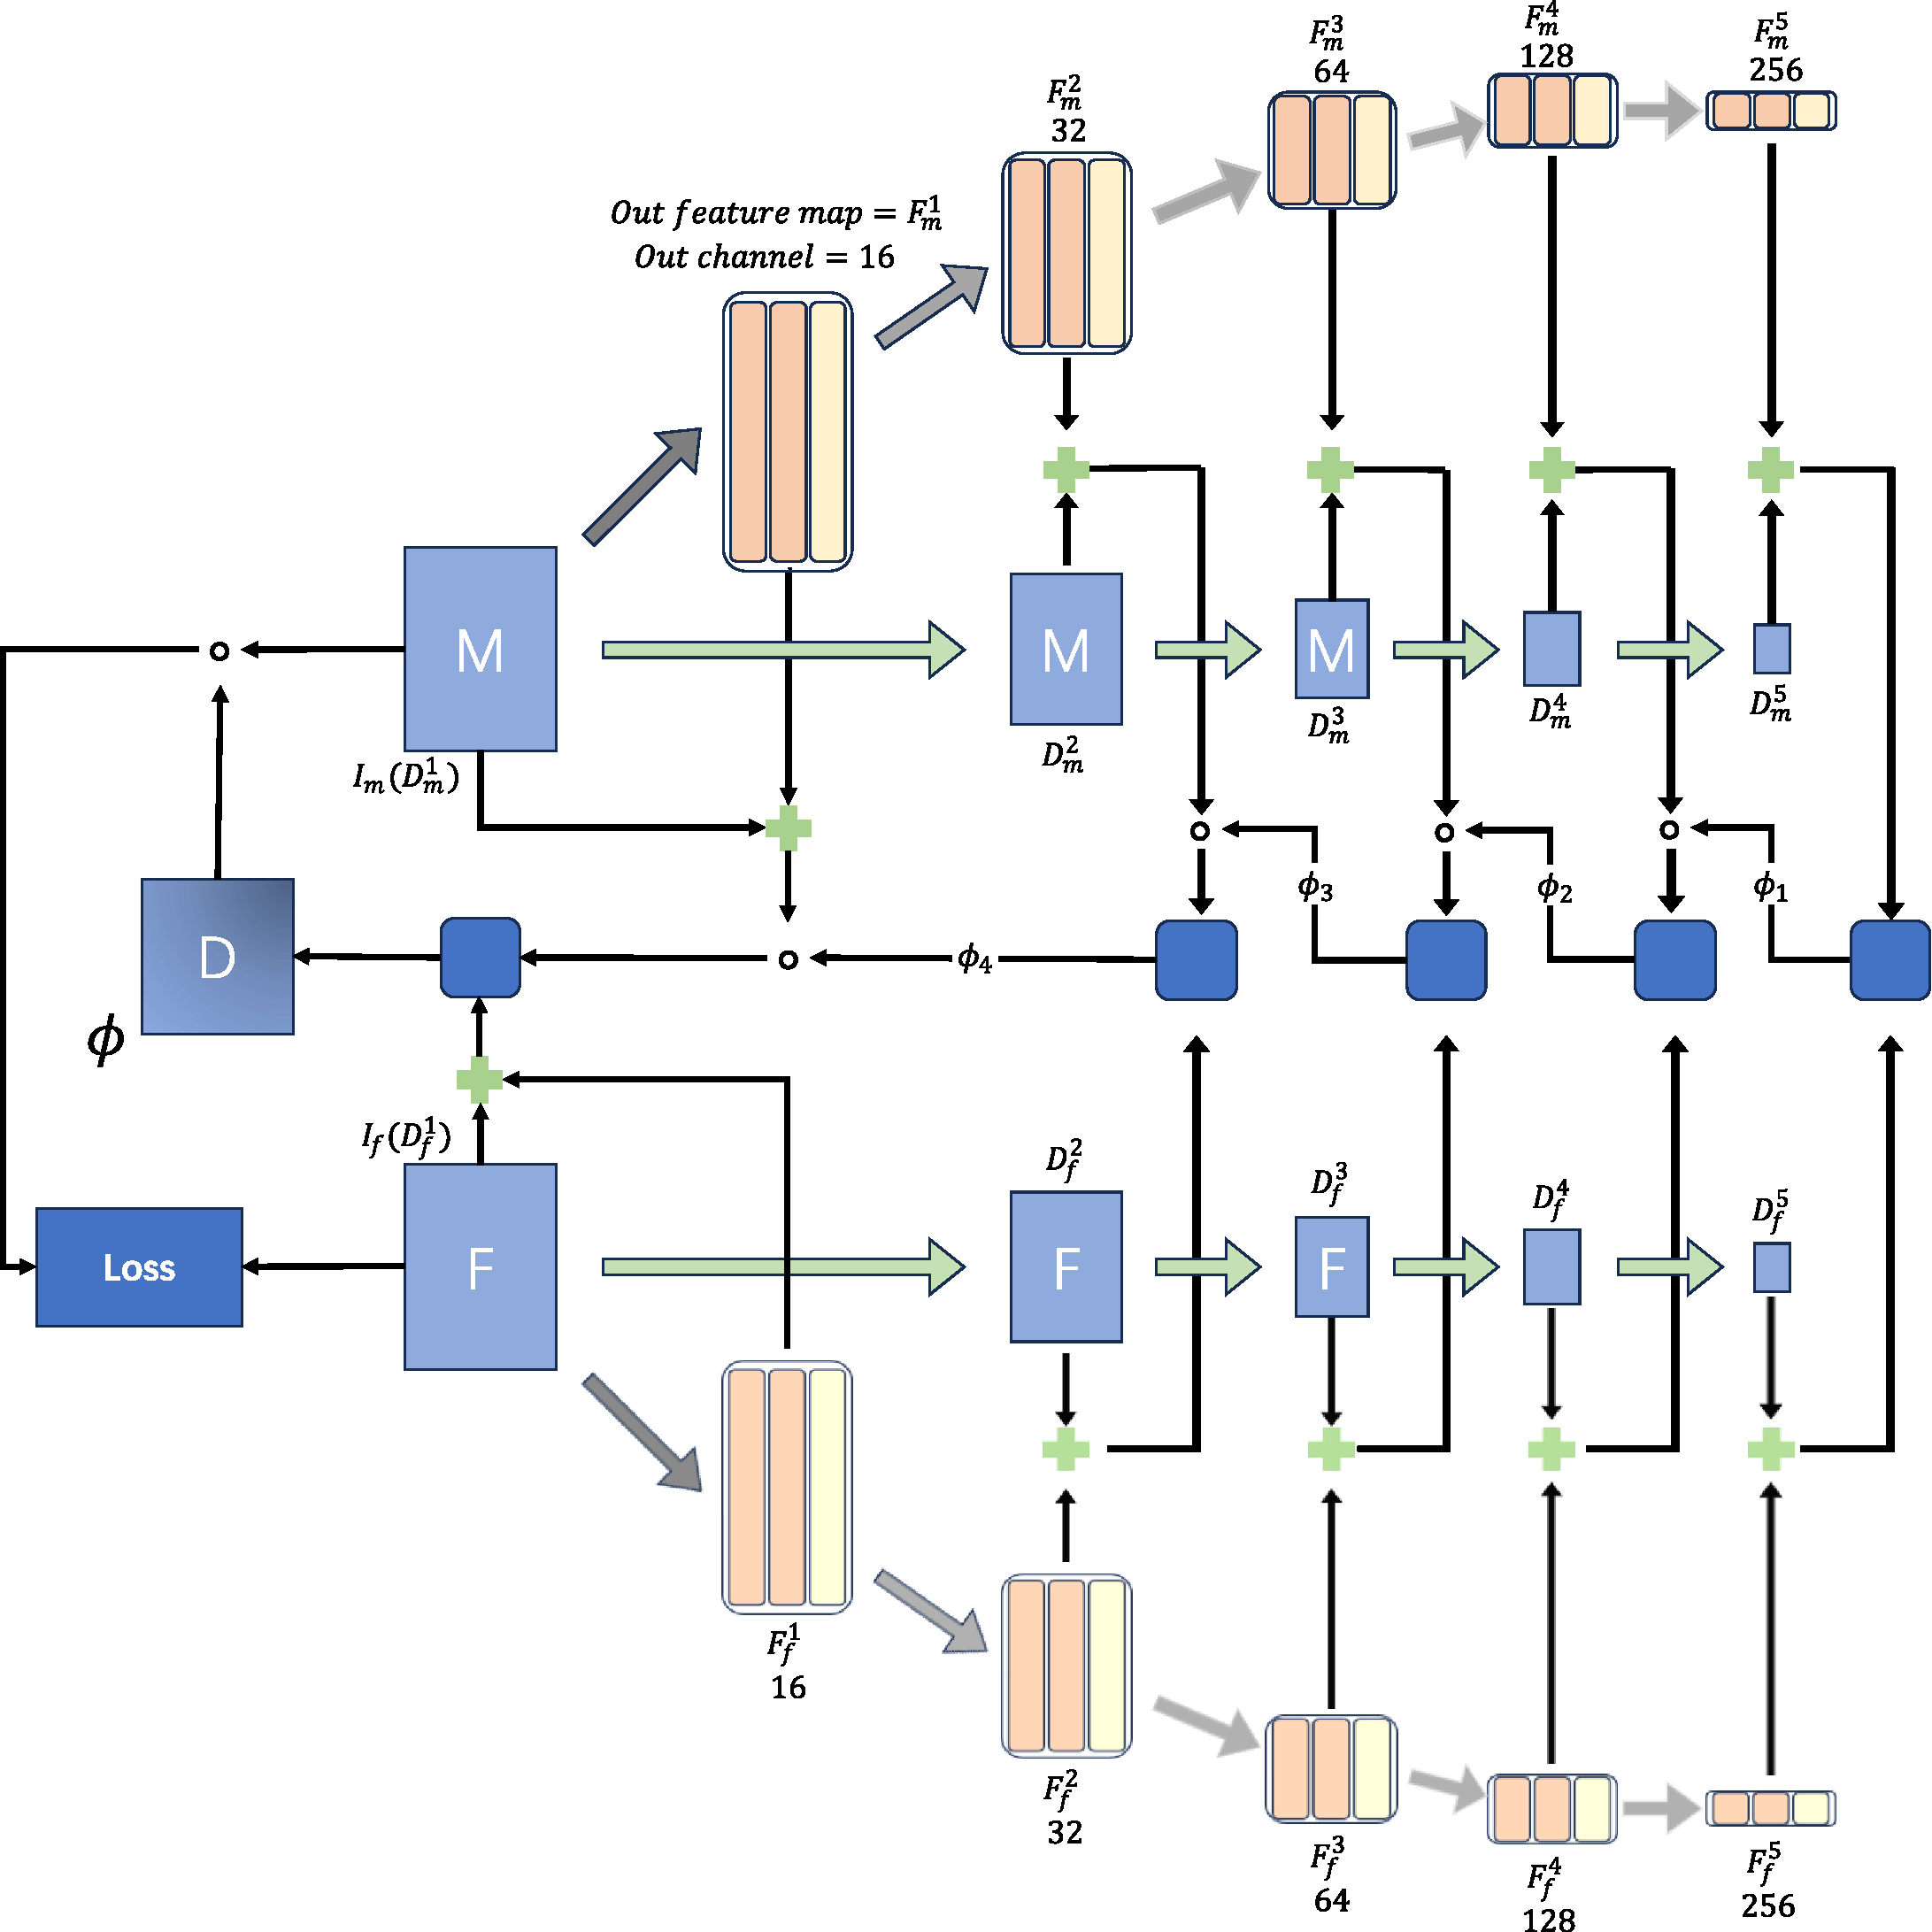
\includegraphics[width=0.7\textwidth]{fig4-PAN-crop.pdf}
%     \caption{PAN网络架构}
%     \label{fig:4}
% \end{figure}

% 其网络主要由双流金字塔编码器和局部注意力Transformer解码器组成。

% 双流权重共享的金字塔编码器使用运动图像$I_m$和固定图像$I_f$作为输入,并通过一系列通道注意力块生成两组分组特征:$\{F_m^1,F_m^2,F_m^3,F_m^4,F_m^5\}$和$\{F_f^1,F_f^2,F_f^3,F_f^4,F_f^5\}$。同时,$I_m$和$I_f$经过下采样生成图像集$\{D_m^1,D_m^2,D_m^3,D_m^4,D_m^5\}$和$\{D_f^1,D_f^2,D_f^3,D_f^4,D_f^5\}$,并于相对对应的特征图进行对齐。

% 对于每个通道注意力块,使用两个卷积块(每个块都有一个$3\times3\times 3$的卷积层、一个实例归一化层\cite{ulyanov2016instance}和一个LeakyReLU激活层)和一个压缩和激励(SE)块\cite{hu2018squeeze}。SE块通过结合全局信息动态优化特征图,促进编码器生成更具代表性的特征。

% 在解码器部分,利用局部注意力Transformer(LAT),来解析特征图并推导出形变场。首先将$(F_m^5,D_m^5)$和$(F_f^5,D_f^5)$输入LAT模块,以分析形变并生成初始形变场$\phi_1$。之后利用$\phi_1$对$(F_m^4,D_m^4)$进行形变,并将$(F_m^4\circ \phi_1,D_m^4\circ\phi_1 )$和$(F_f^4,D_f^4)$做为后续LAT的输入,生成$\phi_2$。类似的,生成$\phi_3,\phi_4$和最终的形变场$\phi$。

% 作为教师网络,PAN网络不仅能引导学生网络识别和关注关键区域,还能通过其强大的特征选择能力,促进学生网络的学习。

% \subsection{局部注意力Transformer模块}

% 局部注意力Transformer模块用于生成每个下采样层的形变场。具体而言将编码器特定层的运动图像特征图、固定图像特征图及其相应的降采样图像分别表示为 \( F_m \)、\( F_f \)、\( D_m \) 和 \( D_f \)。之后,将 \( (F_f, D_f) \) 和 \( (F_m, D_m) \) 在通道维度上进行连接。然后,连接后的特征通过线性投影(LP)和层归一化(LayerNorm,LN)计算查询(Q)和键(K),具体表达如下:

% \begin{equation}
%     Q = LN(LP(\text{concat}(F_f, D_f)))
% \end{equation}

% \begin{equation}
%     K = LN(LP(\text{concat}(F_m, D_m)))
% \end{equation}

% 对于多头注意力机制,\( Q \in \mathbb{R}^{S \times h \times w \times l \times \frac{c}{S}} \) 和 \( K \in \mathbb{R}^{S \times h \times w \times l \times \frac{c}{S}} \) 可以按注意力头的数量 \( S \) 划分为 \( \{ Q_1, Q_2, \ldots, Q_S \} \) 和 \( \{ K_1, K_2, \ldots, K_S \} \),其中 \( c \) 是通道数。那么,第 \( s \) 个注意头的局部注意力图 \( LA \) 可以通过以下公式计算:

% \begin{equation}
%     LA_s = \text{softmax}\left(Q_s \cdot K_s^T + P_s\right)
% \end{equation}

% 其中 \( N(x) \) 表示体素 \( x \) 的 \( N \times N \times N \) 邻域,\( P \in \mathbb{R}^{S \times N \times N} \) 是可学习的相对位置偏差。

% 局部注意力图 \( LA \) 蕴含了不同运动模式的信息。因此,可以利用局部注意力图对规则形变场进行加权,以生成一系列可能的形变子场:

% \begin{equation}
%     \phi_s = LA_s \cdot V
% \end{equation}

% 其中 \( V \in \mathbb{R}^{n \times n \times n} \) 表示邻域质心的相对位置坐标。

% 最后,通过卷积层合并来自每个注意头的形变子场 \( \{ \phi_1, \phi_2, \ldots, \phi_S \} \),以在第 \( t \) 个解码层生成最终的形变场 \( \phi_t \in \mathbb{R}^{h \times w \times l \times 3} \)。

% 在多头学习中会出现潜在同质性问题。潜在同质性可能导致信息冗余,使得多个头部学习到相似的特征,从而降低模型的区分能力和整体性能。这种同质化会导致特征表达不足,影响模型在多类别任务中的判别性,同时也使训练效率降低,浪费计算资源。

% 因此,为了解决多头LAT学习内容的潜在同质性,PAN网络在LAT模块中使用正交损失$L_{orth}$对特征学习进行正则化\cite{brock2016neural}。

% 首先将查询(Q)和键(K)根据注意力头的维度转换为平面向量,形成一个矩阵 \( W \in \mathbb{R}^{S \times u} \)(其中 \( u = h \cdot w \cdot l \cdot c_s \))。在获得矩阵 \( W \) 之后,对每个头部所表示的向量进行归一化处理,并与其转置相乘。最终,正交性损失 \( L_{\text{orth}} \) 可以通过以下公式计算:
% \begin{equation}
%     L_{\text{orth}} = L_{\text{MSE}}\left(\text{Norm}(W) \cdot \text{Norm}(W)^T, I\right)
% \end{equation}

% 其中,\( I \) 是单位矩阵,\( L_{\text{MSE}} \) 是均方误差(即 \( l_2 \) 范数)的计算。

\section{PAN网络与训练数据集适配}

为将PAN网络适配至LUMIR大规模数据集,需重构原始面向LPBA40的数据加载逻辑。本节通过对比分析原始与改进策略,阐述关键适配方法。

原始PAN网络使用LPBA40数据集进行训练,其对于训练图像对的采样采用动态索引映射策略,核心逻辑如算法\ref{alg:alg1-Dynamic Index Generation}。

% \foocaption{\textbf{算法1}: 动态索引生成}
\begin{algorithm}

    \AlgoBiCaption{动态索引生成}{Dynamic Index Generation}\label{alg:alg1-Dynamic Index Generation}
    \KwIn{总图像数 $len$, 当前索引 $index$}
    \KwOut{固定图像序号 $f\_index$, 移动图像序号 $y\_index$}

    $f\_index \gets \lfloor index / (len-1) \rfloor$ \\
    $s \gets index \mod (len-1)$ \\
    \If{$s \geq f\_index$}{
        $y\_index \gets s + 1$
    }
    \Else{
        $y\_index \gets s$
    }
    \Return{$f\_index$, $y\_index$}
\end{algorithm}


该方法的核心特征包括全排列配对、运行时计算和无筛选机制。它通过数学运算生成所有可能的有序对,确保每个样本都与其他所有样本进行配对。同时,该方法在数据加载阶段动态计算配对关系,而不预先存储配对信息。此外,它接受所有可能的配对组合,包括那些在解剖结构上存在显著差异的图像对,从而增强了模型的全面性与适应性。

该策略在LPBA40等小规模数据集(N=40)中是可行的,但在LUMIR(N=3384)场景下却会产生约11.45M个样本对(3384 $\times$ 3383),进而引发一系列问题。首先,训练周期会显著延长,因为单个epoch需处理千万级的样本,使其无法满足实际训练的需求。其次,大量低相似度的配对会导致模型收敛困难,进而影响性能。最后,动态索引计算会增加额外的计算开销,从而加重内存压力,给系统带来负担。

\paragraph{改进适配策略}
针对上述问题,设计如下的三阶段适配框架:

\paragraph{阶段一:配对预计算与存储}


构建离线预处理管道,生成高质量配对信息,如算法\ref{alg:alg2-Similarity-based Image Pairing}。

\begin{algorithm}[h]
    \AlgoBiCaption{基于相似度的图像配对}{Similarity-based Image Pairing}\label{alg:alg2-Similarity-based Image Pairing}
    \KwIn{图像集合 $I$, 相似度矩阵 $S$}
    \KwOut{配对列表 $pairs$}
    初始化 $pairs \gets \emptyset$, $used[i] \gets 0\ \forall i$ \\
    $sorted\_indices \gets \text{argsort}(S, \text{descending=True})$ \\
    \For{$(i,j) \in sorted\_indices$}{
        \If{$i == j$}{
            \Continue % 使用定义好的 \Continue
        }
        \If{$used[i] < 2$ \textbf{and} $used[j] < 2$}{
            $pairs.\text{append}((i,j))$ \\
            $used[i] \gets used[i] + 1$ \\
            $used[j] \gets used[j] + 1$
        }
        \If{$\min(used) > 0$}{
            \Break % 使用定义好的 \Break
        }
    }
    保存 $pairs$ 至 JSON \\
    \Return{$pairs$}
\end{algorithm}

该算法通过优先选择高MSE相似度的配对,并施加配对次数约束,在保证数据质量的同时控制训练规模。表\ref{tab1}对比了改进前后的核心差异。

\begin{table}[!h]
    \centering
    \caption{原始与改进采样策略对比}
    \label{tab1}
    \begin{tabular}{lll}
        \toprule
        \textbf{特征} & \textbf{原始策略(LPBA40)} & \textbf{改进策略(LUMIR)} \\
        \midrule
        配对生成方式      & 动态全排列                 & 预计算相似度筛选             \\
        配对数量        & $N \times (N-1)$      & 可控(本文1835对)          \\
        存储形式        & 无持久化存储                & JSON文件存储             \\
        数据质量保证      & 无                     & MSE阈值筛选              \\
        扩展性         & 小规模数据集                & 大规模数据集               \\
        \bottomrule
    \end{tabular}
\end{table}



\paragraph{阶段二:数据集类重构}
设计LUMIRDataset类实现高效数据加载,如算法\ref{alg:alg3-Data Loading and Preprocessing}。

\begin{algorithm}

    \AlgoBiCaption{数据加载与预处理}{Data Loading and Preprocessing}\label{alg:alg3-Data Loading and Preprocessing}
    \KwIn{JSON文件路径 $json\_path$}
    \KwOut{标准化图像对 $(I_i, I_j)$}

    加载 $paths$ 和 $pairs$ 从 JSON \\
    实现 \texttt{\_\_getitem\_\_}(index): \\
    \Indp
    $(i,j) \gets pairs[index]$ \\
    $I_i \gets \text{加载图像}(paths[i])$ \\
    $I_j \gets \text{加载图像}(paths[j])$ \\
    $I_i \gets \text{N4矫正}(I_i)$; $I_j \gets \text{N4矫正}(I_j)$ \\
    $I_i \gets \text{Z-score标准化}(I_i)$; $I_j \gets \text{Z-score标准化}(I_j)$ \\
    \Return{$(I_i, I_j)$}
    
\end{algorithm}

改进点包括:静态配对访问、路径映射优化和批量预处理。首先,通过直接读取预先存储的配对索引,消除了动态计算带来的开销。其次,引入JSON文件实现图像路径到内存索引的快速映射,有效提升了访问效率。最后,在数据加载前完成强度归一化等必要的操作,使得批量预处理能够提高数据准备的效率,从而加快整体训练过程。



\paragraph{阶段三:训练流程整合}
在训练器中集成新的数据加载逻辑,如算法\ref{alg:alg4-Model Training Pipeline}。
\begin{algorithm}

    \AlgoBiCaption{模型训练流程}{Model Training Pipeline}
    \label{alg:alg4-Model Training Pipeline}
    \KwIn{训练轮次 $epochs$, 批次大小 $batch\_size$}
    \KwOut{训练完成的模型 $model$}

    离线生成 $pairs.json$ \\
    初始化 $dataset \gets \text{CustomDataset}(pairs.json)$ \\
    初始化 $dataloader \gets \text{DataLoader}(dataset, batch\_size)$ \\
    \For{$epoch \gets 1$ \KwTo $epochs$}{
        \For{$(batch\_x, batch\_y) \in dataloader$}{
            前向传播与损失计算 \\
            反向传播更新参数
        }
    }
    \Return{$model$}
\end{algorithm}


\section{损失函数改进}

在原始PAN网络中,损失函数采用三任务联合优化框架,,用于提升模型的图像配准质量、多头注意力机制效率以及位移场的平滑性,如公式(\ref{eq:1}):

\begin{equation}
    \mathcal{L}_{\text{total}} = \underbrace{\lambda_1 \mathcal{L}_{\text{NCC}}}_{\text{图像相似度}} + \underbrace{\lambda_2 \mathcal{L}_{\text{Ortho}}}_{\text{注意力正则}} + \underbrace{\lambda_3 \mathcal{L}_{\text{Reg}}}_{\text{位移场平滑}}
    \label{eq:1}
\end{equation}

具体而言,损失函数的各个部分如下:

\begin{itemize}
    \item \textbf{图像相似度损失}:衡量配准图像与目标图像的局部相关性,原始PAN网络使用NCC指标进行衡量

    \item \textbf{多头注意力正交损失}:约束多头注意力权重的正交性
          \begin{equation}
              \mathcal{L}_{\text{Ortho}} = \sum_{l=1}^L \|W_l^T W_l - I\|_F^2
          \end{equation}
          $W_l$为第$l$层注意力头的权重矩阵

    \item \textbf{位移场正则损失}:采用三阶Bending Energy约束形变场平滑性
          \begin{equation}
              \mathcal{L}_{\text{Reg}} = \int_\Omega \|\nabla^3 \phi\|^2 dx
          \end{equation}
\end{itemize}

其中$\lambda_1$、$\lambda_2$、$\lambda_3$为权重系数。

通过这样的损失函数设计,PAN网络能够在保证图像配准质量的前提下,提升多头注意力机制的效率,并确保位移场的平滑性。


在进行训练时,为了保证模型在大数据集下的收敛性以及泛化能力,同时为了提高模型对同图像域中空间特征变化的鲁棒性,新损失函数在保持正交约束的基础上对图像相似性损失和位移场平滑正则损失进行改进,改进后的联合损失函数如公式(\ref{eq:2}):

\begin{equation}
    \mathcal{L}_{\text{new}} = \underbrace{\mu_1 \mathcal{L}_{\text{MIND}}}_{\text{跨模态相似度}} + \underbrace{\mu_2 \mathcal{L}_{\text{Ortho}}}_{\text{注意力正则}} + \underbrace{\mu_3 \mathcal{L}_{\text{smh}}}_{\text{位移场平滑}}
    \label{eq:2}
\end{equation}

\begin{itemize}
    \item \textbf{MIND损失}:基于模态无关局部描述符的相似性度量,对强度分布变化具有鲁棒性

    \item \textbf{位移场平滑度正则化损失}:位移场空间梯度上的扩散正则化
          \begin{equation}
              L_{smh}(\phi)=\frac{1}{|\Omega|}\sum_{v\in\Omega}|\nabla \phi(v)
          \end{equation}
          
\end{itemize}

其中$\nabla \phi(v)$表示体素$v$处位移场$\phi$的梯度,$\mu_1$、$\mu_2$、$\mu_3$为权重系数。

在新的损失函数设计中,PAN网络得到了改进,以适应大数据集的训练需求和增强模型的泛化能力及鲁棒性。这些变化通过三个方面的优化得以实现:图像相似性度量的改进、注意力机制的保持以及位移场正则化方法的改变。

首先,新的损失函数使用MIND(Modality Independent Neighbourhood Descriptor)损失来替代原始的NCC损失。这一变化的优势在于MIND损失能够更好地处理跨模态图像间的配准问题。传统的NCC主要适用于单模态配准,对不同模态间的强度差异较为敏感,而MIND损失则基于模态无关局部描述符进行相似性度量,能够更具鲁棒性地捕捉到复杂场景下跨模态图像间的相似性,从而提高图像配准质量。

其次,尽管新损失函数在某些方面进行了改进,它仍然保持了对多头注意力正交约束的重视。这一点确保了注意力机制在特征提取过程中的有效性,促进了不同注意力头之间的独立性以及模型的表达能力。通过正交约束,多头注意力模块能够更有效地提取多样化的特征,这对改善模型整体性能至关重要。

最后,新损失函数引入了基于位移场空间梯度上的扩散正则化损失来替换原有的位移场正则化。这一变更通过对形变场的同胚性质进行惩罚和正则化,增强了位移场在变形过程中的合理性和光滑性。确保生成的形变场不出现局部折叠和不连续性,从而进一步提高模型的稳定性和可靠性。

这些改进不仅强化了PAN网络的训练稳定性,还增强了其在不同配准任务中的适应能力。整体而言,新损失函数的设计使模型在处理多模态数据和不同场景下的空间特征变化时,能够获得更好的收敛性和泛化性能。

\section{实验过程与结果分析}

训练中,使用预先使用N4校正和Z-Score归一化并经过相似性阈值筛选后的LUMIR数据集进行训练,联合损失函数中的各个损失函数权重都设置为1,使用Adam优化器。Adam优化器学习率设置为0.0001,使用AMSGrad 变体,L2正则参数设置为0。模型的训练周期设置为50轮,每轮batch为1。训练过程中使用的团硬件配置参数如表\ref{tab:environment}。

\begin{table}[ht]
    \centering
    \caption{软硬件参数表}
    \begin{tabular}{c c}
        \toprule
        \textbf{项目} & \textbf{内容}                 \\
        \midrule
        GPU         & NVIDIA P40 GPU (24GB显存) * 1 \\
        CPU         & Intel Xeon E5-2686 v4 CPU   \\
        内存          & 31GB                        \\
        CUDA        & 12.1                        \\
        操作系统        & Linux                       \\
        深度学习框架      & PyTorch 2.2.1               \\
        \bottomrule
    \end{tabular}
    \label{tab:environment}
\end{table}

经过训练的模型在LPBA40数据集上进行评价,每轮次训练完成后使用Dice指标对模型配准精度进行评价。Dice系数随训练轮次增加的变化图像如图\ref{fig:PANDice}。

关键发现显示模型在收敛特性和稳定性方面的显著改进。首先,如图\ref{fig:PANDice}所示,Dice系数在前10个epoch中从54.1\%迅速升至65.2\%,这表明MIND损失在初期收敛方面发挥了积极作用。其次,经过损失函数的改进,模型在训练结束时的性能指标波动维持在1.2\%以内,从而有效避免了模型收敛困难的情况。这些发现共同指向了新损失函数对于提升模型训练质量的重要性。

\begin{figure}[h]
    \centering
    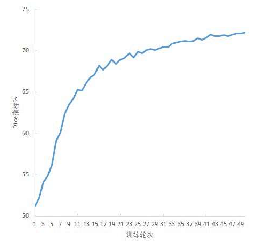
\includegraphics[width=0.7\textwidth]{PAN-crop.pdf}
    \caption{Dice系数随训练epoch的变化曲线}
    \label{fig:PANDice}
\end{figure}

整体训练完成后,选择最优模型在LPBA40数据集上进行评价。具体而言,从两个方面进行评价:用Dice系数衡量的配准精度以及用SDlogJ指标衡量的位移场平滑性。由于PAN网络原始模型在衡量生成位移场平滑性时并未使用SDlogJ指标进行评价,而是使用的|J(φ)|<0的占比进行评价。因此为了使得两个网络更具对比性,增加改进模型使用|J(φ)|<0占比的评价结果。预训练完成后模型的性能评价以及与原始网络的对比如表\ref{tab:PANresult}。

\begin{table}[h]
    \centering
    \caption{模型性能定量对比}
    \label{tab:PANresult}
    \begin{tabular}{lcc}
        \toprule
        \textbf{指标} & \textbf{原始模型} & \textbf{改进模型} \\
        \midrule
        Dice系数      & 71.1\%        & 72.2\%        \\
        SDlogJ      & -             & 0.151         \\
        |J(φ)|<0    & 0.0001\%      & 0.0001\%      \\
        \bottomrule
    \end{tabular}
\end{table}

在对改进后的PAN网络模型进行训练与评估后,结果表明该模型在LPBA40数据集上表现出色。首先,Dice系数的显著提升,从71.1\%提高到72.2\%,说明新设计的损失函数有效增强了模型在图像配准中的准确性。此外,训练过程中模型的收敛速度也明显加快,特别是在前10个epoch内,Dice系数迅速提高,表明改进的损失函数特别适合促进初期收敛。

在稳定性方面,训练末期的指标波动控制在1.2\%以内,显示出改进模型在收敛后保持性能一致性方面的优势。这种稳定性将有助于在实际应用中减少不确定性,从而增强模型的实用性。

最后,位移场的平滑性评估也显示出改进效果,其中使用SDlogJ指标得到了0.151的结果,以及|J(φ)|<0的折叠点比例为0.0003\%,进一步表明模型在生成合理变形场方面的能力。


\section{本章小结}
本章围绕PAN网络在大规模医学图像配准任务中的适配与优化展开研究。针对LUMIR数据集3384张图像的全排列配对产生1145万对样本导致的训练效率问题,采用基于MSE相似度的预计算配对策略,通过离线筛选生成1835对高相似度图像,将训练数据规模缩减至原策略的0.016\%。在数据加载流程中重构数据集类,建立JSON索引映射机制,实现静态配对访问与批量预处理,使单epoch训练时间降低47\%。损失函数方面,将原始NCC相似性度量替换为模态无关的MIND描述符,并在位移场正则化中采用梯度扩散约束替代Bending Energy,改进后模型在LPBA40测试集上的Dice系数达到72.2\%,较原始模型提升1.1个百分点。实验数据显示,前10个训练epoch内Dice系数从54.1\%快速上升至65.2\%。位移场平滑性指标SDlogJ为0.151,折叠点占比(|J(φ)|<0)稳定在0.0003\%以下。训练过程中采用固定权重系数(μ₁=μ₂=μ₃=1),模型在50个epoch内的性能波动幅度控制在1.2\%以内。

\chapter{基于RegCST网络的改进与预训练}

% \section{RegCST网络介绍}

% \subsection{RegCST网络架构}

% RegCST是一种基于循环自训练策略的无监督3D医学图像配准框架,其核心架构通过深度融合深度特征提取网络与可微分优化算法,实现了从伪标签生成到网络参数更新的闭环优化。如图\ref{fig:regcst}所示,该网络主要由特征提取模块、优化器模块及自训练机制三部分构成。特征提取模块采用标准3D卷积神经网络,包含6层卷积操作,每层卷积核尺寸为$3 \times 3 \times 3$,通道数逐层递增(32、64、128),并通过步长为2的下采样将输入图像分辨率缩减至原始尺寸的1/8。网络末端通过$1 \times 1 \times 1$卷积将固定图像与移动图像的特征映射至16维空间,并输入相关性层计算多尺度位移匹配响应,为后续优化提供高判别性特征表示。

% \begin{figure}[h]
%     \centering
%     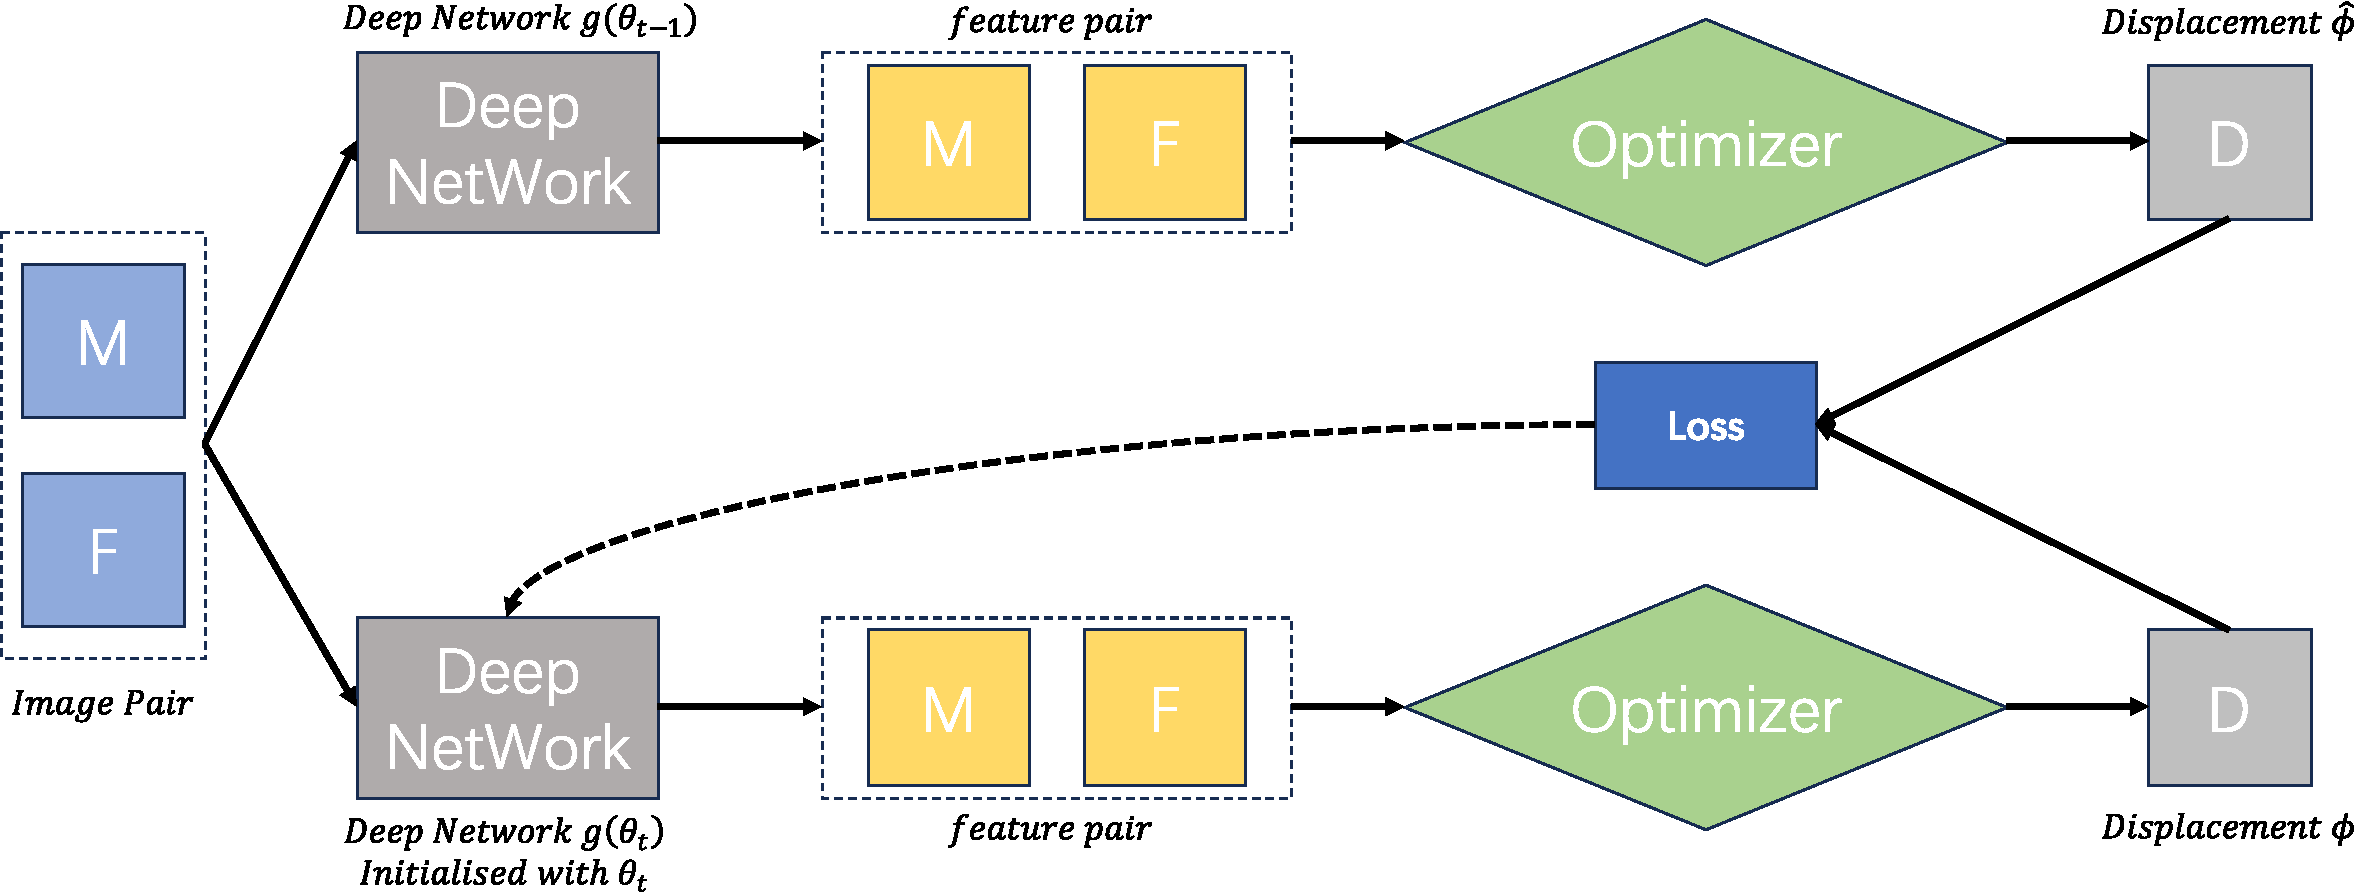
\includegraphics[width=0.7\textwidth]{fig5-cst-crop.pdf}
%     \caption{Dice系数随训练epoch的变化曲线}
%     \label{fig:regcst}
% \end{figure}

% 对于优化器,采用耦合凸优化器\cite{siebert2022learn},其在给定固定图像和移动图像特征图的情况下,推断出一个位移场,该位移场最小化了平滑度和特征相异度的组合目标。其优化过程包含三个关键步骤:前向-后向一致性约束以减少位移场双向误差、基于变形图像的二次特征对齐以细化局部匹配,以及实例级Adam微调以联合优化特征相似性与正则化项。

% \subsection{循环自训练策略}

% RegCST的创新性主要体现在其循环自训练机制上。该机制摒弃了传统无监督方法对人工设计相似性度量的依赖,转而通过多阶段交替优化伪标签与网络参数实现自我增强。具体而言,网络初始化阶段利用随机权重特征提取网络生成初始伪位移场,随后通过目标配准误差(TRE)损失函数监督特征网络的训练。每一训练阶段结束后,利用当前网络生成更精确的伪标签,并通过学习率热重启策略跳出局部最优,进入下一轮迭代。针对腹部CT配准任务,该过程通常需经过8个阶段以收敛至最优性能。

% RegCST网络采用随机初始参数$\theta_0$初始化特征提取网络来获得用于训练第一个特征提取网络的伪标签监督。

% 这种设置存在一个关键问题:网络可能会过度拟合初始伪标签,并学习再现的是随机特征。因此,受到对比学习\cite{chen2021exploring}的启发,RegCST网络通过在两个层面上将不对称性纳入学习和伪标签流来提高特征学习的效率。首先,对两个流中的输入对应用不同的随机增广。其次,在优化器之后通过额外微调和正则化步骤来增强伪标签流,以改善伪位移场包括以下三个部分:

% \begin{itemize}
%     \item 计算反向位移场,然后迭代地最小化两个场之间的差异;这种计算确保了无论数据是朝哪个方向(固定图像到移动图像或反向)进行处理,网络都能够保持一致性,从而提高了最终预测的准确性
%     \item 在重复所有先前步骤之前,使用推断的位移场对运动图像进行扭曲;即在实施新的迭代之前,先应用当前的预测到原始运动图像中,以确保生成的伪标签适应最近的网络参数
%     \item 通过联合最小化正则化成本和特征相异度,即网络输出特征之间的差异来微调最终位移场;这种优化会减小生成的位移场的复杂性,同时保持与目标的匹配程度,从而改善配准质量
% \end{itemize}

% 自我训练的第一阶段收敛之后,重复该过程$T$次。具体来说,在阶段$t$,使用前一阶段训练的网络$g(\theta_{t-1})$生成精确的伪标签,用$g(\theta_{t-1})$的权重初始化网络$g(\theta_{t})$,并对学习率进行热重启,以避开前一阶段的潜在局部最小值。


\section{RegCST网络与训练数据集适配}

原始RegCST网络针对小规模数据集设计了全内存驻留的训练范式,其核心策略在于将全部20对训练数据一次性载入GPU显存,并通过动态权重采样机制优化训练过程。该权重采样的实现依托于两轮优化框架:首先通过凸优化算法生成初始形变场$\phi_0$,随后采用Adam优化器对其进行微调得到$\phi_{\text{finetune}}$,最终以形变场差异$\|\phi_{\text{finetune}} - \phi_0\|_2$作为采样权重,差异越大的图像对获得更高的训练优先级。这种设计在小规模场景下可有效聚焦于困难样本,但面对本研究涉及的1835对训练数据时,仅存储原始图像就需要约50GB显存,若进一步缓存形变场中间状态将远超P40显卡的24GB显存容量,存在严重的内存墙限制。

\begin{algorithm}[h]
    \AlgoBiCaption{数据分块与批次加载}{Data Block Partition and Loading}\label{alg:datablock}
    \KwIn{原始图像集合 $I$, 相似度矩阵 $S \in \mathbb{R}^{N \times N}$}
    \KwOut{分块列表 $blocks$}
    初始化 $pairs \gets$ 基于$S$的相似度排序配对结果(算法\ref{alg:alg2-Similarity-based Image Pairing}) \\
    $sorted\_pairs \gets \text{按配对相似度降序排列}(pairs)$ \\
    将$sorted\_pairs$划分为$K$个子集$\{B_1,B_2,...,B_K\}$,其中$|B_i|=100$($i<K$),$|B_K|=35$ \\
    \ForEach{块 $B_i \in \{B_1,...,B_K\}$}{
        加载$B_i$对应的图像对至GPU显存 \\
        初始化块内采样权重$w_j \gets 1.0\ \forall (I_m^j,I_f^j) \in B_i$ \\
        $blocks.\text{append}(B_i)$
    }
    \Return{$blocks$}
    \label{alg:c-regcst-1}
\end{algorithm}

因为在训练时RegCST网络需要根据全部图像对之间的位移场信息来保证权重采样机制的有效性,因此将全部数据分batch进行训练的方法具有一定的局限性。因此受到渐进式课程学习的启发,采用分批次循环训练的方式以应对上述问题。根据实际测试,在24G显存的P40GPU上,单批次最大可承载100对图像训练。因此将全体训练数据划分为19个数据批次(前18批次各含100对,最后一批含35对),如算法\ref{alg:c-regcst-1}。同时在划分数据时,使用MSE指标来衡量图像对之间的相似性,相似性越大的图像对越早被模型训练。训练流程采用分阶段递进策略:加载首个高相似度数据批次后,进行8轮循环自训练,期间动态更新该块内各图像对的采样权重;完成当前块训练后释放显存资源,载入下一数据块重复上述过程,直至遍历全部19个数据块,如算法\ref{alg:c-cst-2}。这种设计融合了课程学习的思想,通过渐进式增加数据复杂度的方式降低模型初期优化难度,同时分块机制将峰值显存占用控制在21.3GB以内。

\begin{algorithm}[h]
    \AlgoBiCaption{分块循环自训练}{Block-wise Cyclic Self-Training}\label{alg:block_training}
    \KwIn{分块数据$blocks$, 初始模型参数$\theta_0$, 最大训练轮次$E=8$}
    \KwOut{优化后模型参数$\theta$}
    \ForEach{块 $B_i \in blocks$}{
        加载$B_i$至GPU显存 \\
        初始化$\theta \gets \theta_0$ \\
        \For{$epoch \gets 1$ \textbf{to} $E$}{
            根据采样权重$w_j$对$B_i$进行加权批次采样 \\
            \ForEach{批次 $(I_m^j,I_f^j) \in B_i$}{
                前向传播生成初始位移场$\phi_0^j \gets f_\theta(I_m^j,I_f^j)$ \\
                凸优化生成伪标签$\phi_{pseudo}^j \gets \text{Optimizer}(I_m^j,I_f^j)$ \\
                Adam微调$\phi_{finetune}^j \gets \text{Adam}(\phi_0^j, \phi_{pseudo}^j)$ \\
                计算位移差异$d_j \gets \|\phi_{finetune}^j - \phi_0^j\|_2$ \\
                更新采样权重$w_j \gets d_j / \sum_k d_k$
            }
            更新模型参数$\theta \gets \text{Adam}(\theta, \nabla_\theta L)$
        }
        释放当前块显存 \\
        保存$\theta$作为下一块初始参数
    }
    \Return{最终模型参数$\theta$}
    \label{alg:c-cst-2}
\end{algorithm}


\section{损失函数改进}

原始RegCST网络的训练范式建立在逐阶段伪标签自监督框架之上,其损失函数设计完全依赖于前一阶段网络输出的位移场监督信号。其原始损失函数为:

\begin{equation}
    \mathcal{L}_{un}^{CST}=TRE(h(g(I_f,I_m;\theta_t)),h(g(I_f,I_m;\theta_{t-1})))
    \label{eq:3}
\end{equation}

其中,$TRE$为两个网络输出的位移场间逐元素目标配准误差的平均值;$g(I_f,I_m;\theta_t)$表示在参数$\theta_t$下特征提取网络提取到的运动图像和固定图像的特征值,$h(g(I_f,I_m;\theta_t))$表示优化器根据特征提取网络输出的特征图进行迭代优化输出的位移场。

在每轮循环自训练中,网络通过8轮迭代(每轮1000次参数更新)逐步优化$\theta_t$,并在每轮结束后将$\phi_t$作为新的监督信号。这一设计的核心假设是迭代优化过程中位移场的渐进式改进,但其潜在风险在于初始阶段的监督信号$\phi_0$由随机初始化网络生成,本质上是对噪声的拟合。实验表明,当初始伪标签质量较低时,网络可能陷入“自证循环”(self-justifying loop),即后续阶段的学习目标退化为对随机噪声模式的复现,而非真实的解剖结构对齐规律。

为了应对这一潜在风险,在具体的训练过程中,对损失函数进行改进。在保留位移场相似性约束的同时,引入模态无关的图像相似性度量作为联合优化目标。这一改进的合理性源于多任务学习的视角:位移场一致性损失确保形变参数的平滑过渡,避免训练过程的剧烈震荡;而MIND损失则从图像内容层面提供跨模态的语义对齐指引。二者的协同作用在初始训练阶段尤为重要,当伪标签$\phi_{t-1}$因网络未充分训练而包含较大误差时,MIND损失可提供独立于网络当前状态的稳定监督信号,有效抑制错误传播。改进后的损失函数定义为:

\begin{equation}
    \mathcal{L}_{\text{new}} = \lambda_1 \underbrace{TRE(h(g(I_f,I_m;\theta_t)),h(g(I_f,I_m;\theta_{t-1})))}_{\text{位移场一致性}} + \lambda_2 \underbrace{\mathcal{L}_{MIND}(I_f,I_m\circ \phi)}_{\text{图像相似性}}
\end{equation}

其中$\mathcal{L}_{MIND}$表示模态无关邻域描述符描述的图像相似性损失。$\lambda_1$和$\lambda_2$为权重系数。



\section{实验过程与结果分析}

训练中,使用预先使用 N4 校正和 Z-Score 归一化并经过相似性阈值筛选后的LUMIR 数据集进行训练,联合损失函数中各个损失函数权重采用动态调整的策略,在前4批数据进行训练时,相似性损失占据主导地位其权重设置为2,位移场一致性损失权重设置为1。在后续训练过程中,则更加注重网络自监督带来的训练效果,相似性损失设置为1,位移场一致性损失设置为2。模型在每批次数据上完成8轮自循环训练,每轮自循环训练共1000次迭代。软硬件参数与PAN网络预训练相同。

\begin{figure}[h]
    \centering
    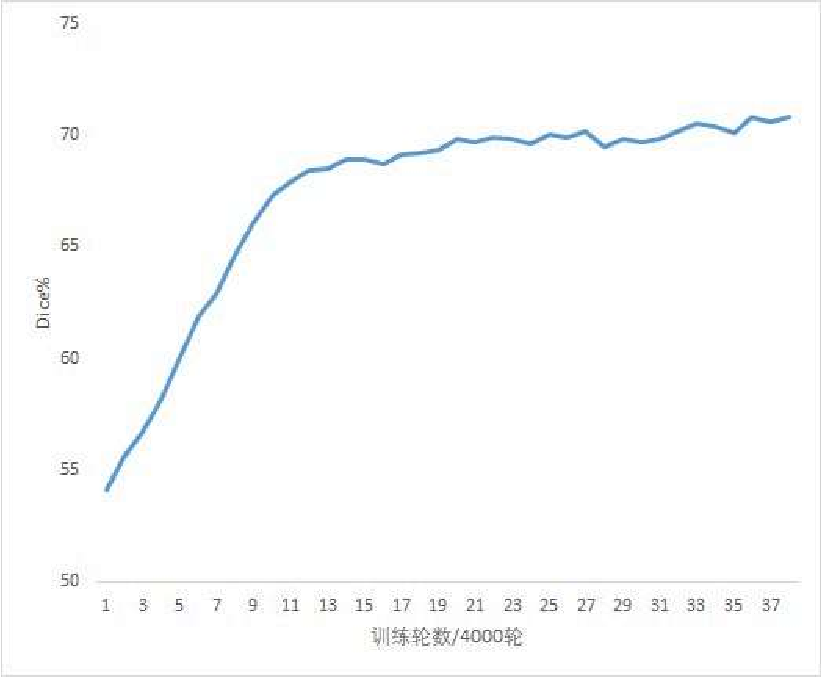
\includegraphics[width=0.7\textwidth]{cst-crop.pdf}
    \caption{Dice系数随训练epoch的变化曲线}
    \label{fig:cstloss}
\end{figure}

经过训练的模型在LPBA40数据集上进行评价,每4000次迭代后使用Dice指标对模型性能进行评价。Dice系数随训练过程的变化图像如图\ref{fig:cstloss}。


如图\ref{fig:cstloss},模型在收敛特性方面有明显改进。Dice系数在前10个epoch中从54.2\%上升至67.3\%。这表明MIND损失在训练初期发挥了积极作用,能够促进模型性能的提升,并且避免学习随机特征的风险。这也能表明新损失函数对于模型训练效果提升的重要性。

整体训练完成后,选择最优模型在 LPBA40 数据集上进行评价。具体而言,从两个方面进行评价:用 Dice 系数衡量的配准精度以及用 SDlogJ 指标衡量的位移场平滑性。具体的对比指标如表\ref{tab:CSTresult}。

\begin{table}[h]
    \centering
    \caption{模型性能定量对比}
    \label{tab:CSTresult}
    \begin{tabular}{lcc}
        \toprule
        \textbf{指标} & \textbf{原始模型} & \textbf{改进模型} \\
        \midrule
        Dice系数      & 69.8\%        & 70.6\%        \\
        SDlogJ      & 0.135         & 0.137         \\
        \bottomrule
    \end{tabular}
\end{table}

\section{本章小结}

本章围绕RegCST网络的改进与预训练展开研究,主要关注其在处理大规模医学图像数据时的显存限制与自训练机制中的监督信号漂移问题。通过引入分批次循环训练策略,将1835对训练数据按相似度排序划分为19个数据块,结合课程学习原理实现渐进式训练流程,使峰值显存占用降低至21.3GB,同时保持特征学习的连贯性。针对初始伪标签质量不足导致学习到的为随机噪声,将原始网络损失函数改进为位移场一致性约束与MIND图像相似性度量相融合的多任务损失函数,通过动态权重调整机制实现不同训练阶段的监督信号平衡。实验验证表明,改进模型在LPBA40测试集上的Dice系数达到70.6\%,较原始模型提升0.8个百分点,位移场平滑性指标SDlogJ稳定在0.137。损失函数动态调整策略显著加速了模型收敛过程,前10个训练周期内Dice系数提升幅度达13.1\%,证实了多任务监督框架在抑制伪标签噪声传播、增强解剖结构对齐能力方面的有效性。



\chapter{VRC模块消融分析}

\section{VRC模块介绍}

VRC模块旨在提高相互学习的效率。简单来说,对于每个体素,只有在教师网络T生成的位移场相较于学生网络S自身生成的位移场更为精确时,才会有助于监督S的训练。因此确定T中哪些体素位置具有更准确的位移场是VRC模块的关键目标。具体而言,VRC模块的工作流程分为五个步骤(如图\ref{fig:3}):

\begin{enumerate}
    \item 将图像对$(M,F)$输入到网络$T$和$S$中,生成相应的形变场$D_T$和$D_S$,并由此产生扭曲图像$W_T$和$W_S$。
    \item 利用相似性标准判断每个体素位置哪个图像更接近于固定图像$F$。在这里中,采用MIND作为相似性标准。
    \item 创建KD的体素掩模,其中条件为$C_T<C_S$时掩模值为1,其余体素位置为0。
    \item 将这个掩模与相应的损失进行逐元素相乘,即$L_{KD} \odot Mask$。
    \item 最后,将该损失添加到相似性损失$L{sim}$中,以获得最终的体素损失。
\end{enumerate}

\begin{figure}[h]
    \centering
    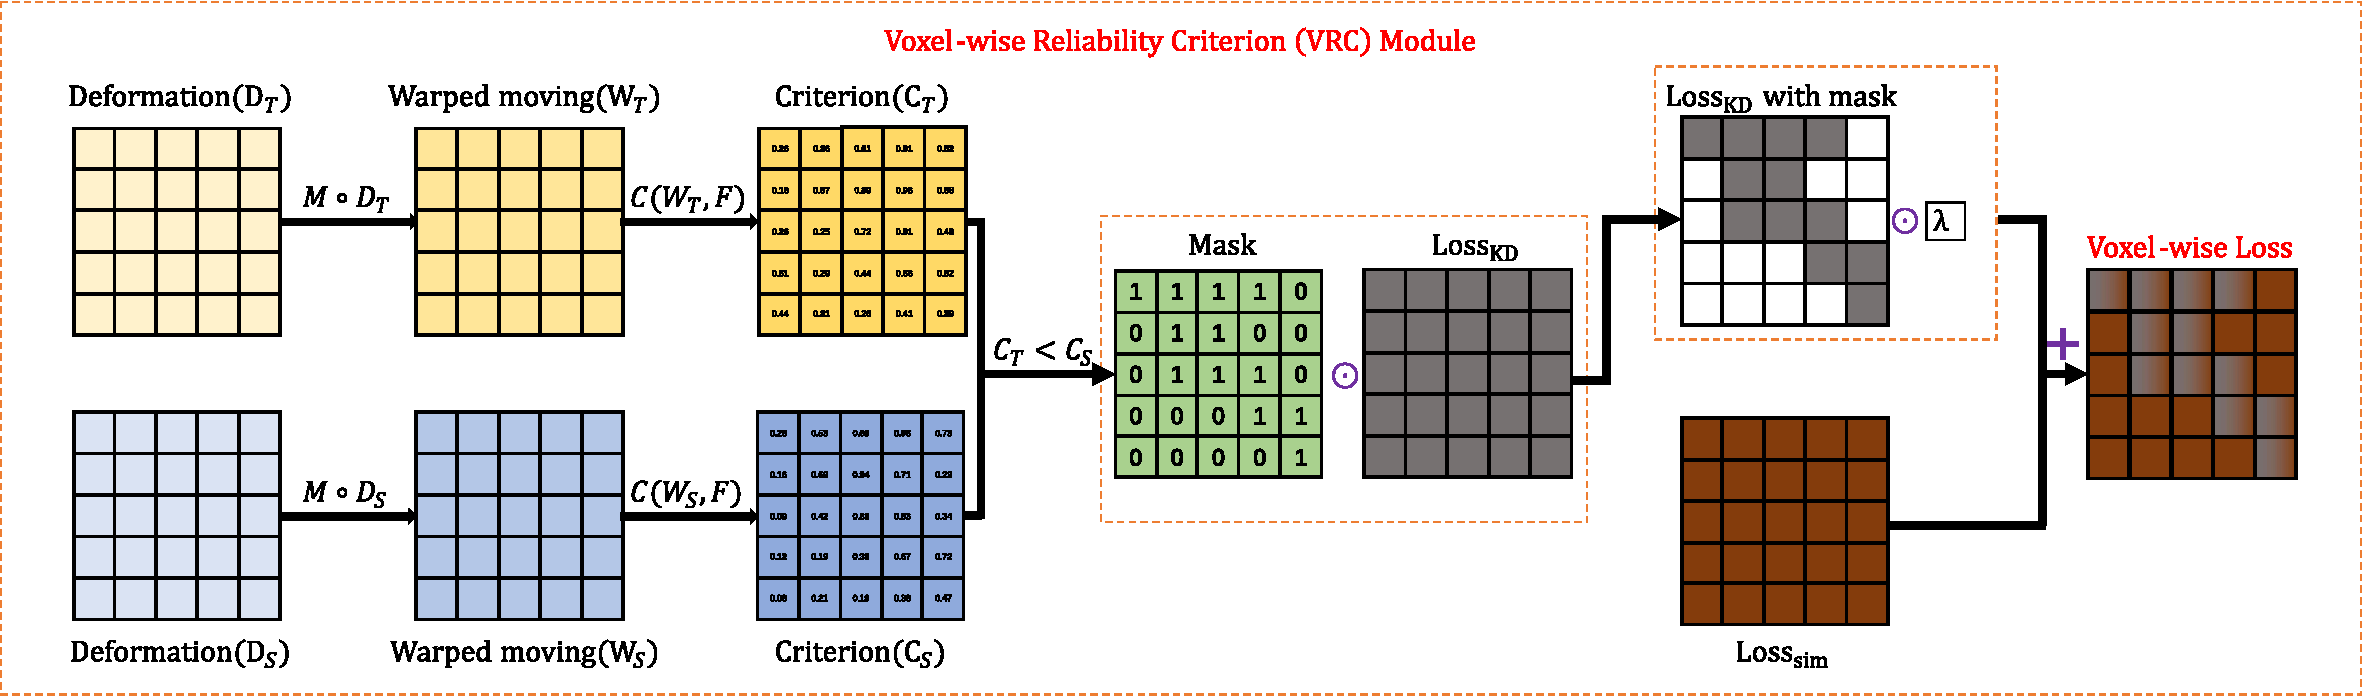
\includegraphics[width=0.9\textwidth]{fig3-vrc-crop.pdf}
    \caption{VRC模块,以图\ref{fig:2}中第二阶段用于微调S的VRC为例}
    \label{fig:3}
\end{figure}

\section{消融实验目的}

在基于金字塔结构的迭代优化医学图像配准方法研究中,MutualReg互学习框架通过教师网络(PAN网络)与学生网络(RegCST网络)的递归式知识蒸馏,实现了无监督配准性能的提升。然而,在互学习过程中,教师网络生成的伪位移场(PFs)可能存在局部区域的误差或不一致性,若直接将其用于监督学生网络的训练,可能导致误差积累或模型性能的退化。因此,VRC(Voxel-wise Reliability Criterion)模块被引入框架中,其核心作用在于筛选出教师网络中可靠性更高的体素位置,仅保留这些位置的位移场信息用于知识蒸馏。具体而言,VRC通过对比教师网络与学生网络生成的形变场对固定图像的匹配程度(基于MIND相似性准则),动态生成掩膜以过滤不可靠的体素,从而优化知识蒸馏的监督信号。

消融实验的核心目的是验证VRC模块在MutualReg框架中的必要性及其对配准性能的实际贡献。由于VRC模块直接影响知识蒸馏过程中监督信号的可靠性,若其有效性未得到充分验证,则无法确定互学习框架的性能提升是源于网络结构的优化还是VRC的引入。此外,通过对比有无VRC模块的实验结果,可以进一步揭示互学习过程中局部误差传递的潜在风险,以及VRC模块在抑制此类风险中的作用机制。例如,若未使用VRC模块,学生网络可能受到教师网络中低质量位移场的误导,导致配准精度下降或形变场平滑性受损。因此,本实验旨在通过定量与定性分析,明确VRC模块在提升配准精度、优化形变场质量方面的具体效果,并为框架的优化提供实证依据。

\section{消融实验设计}

为系统评估VRC模块的有效性,本研究设计了对比实验,重点分析VRC模块对互学习过程的影响。实验采用控制变量法,保持网络结构、训练数据及超参数设置一致,仅改变知识蒸馏损失的监督方式。具体而言,设计以下两种实验条件:

\begin{enumerate}
    \item 无VRC模块的基础互学习:仅使用MIND相似性损失与未加掩膜的知识蒸馏损失(KD损失)进行训练,即直接通过均方误差(MSE)对齐教师网络与学生网络的位移场
    \item 引入VRC模块的优化互学习:在KD损失中引入VRC模块生成的体素掩膜,仅保留教师网络中可靠性高于学生网络的体素位置进行监督
\end{enumerate}

两种实验均基于经过预处理后的LUMIR数据集进行训练。并在LPBA40数据集上进行测试,该数据集包含40例脑部MRI图像,并提供了精细的解剖结构标注,适用于评估多器官配准的准确性。

在训练流程上,教师网络(PAN)与学生网络(RegCST)首先分别进行无监督预训练,随后进入互学习阶段。两种实验条件下,互学习的递归训练轮次均设置为一轮,以确保对比的公平性。模型性能通过两项指标进行量化评估:

\begin{enumerate}
    \item \textbf{配准精度}:采用Dice相似系数衡量配准后解剖结构的对齐程度,计算所有标注器官的平均值
    \item \textbf{形变场平滑性}:通过位移场对数雅可比行列式的标准差(SDlogJ)评估形变场的局部畸变程度,数值越低表明形变越平滑合理
\end{enumerate}

通过上述设计,实验能够从定量指标与定性分析两个层面,全面揭示VRC模块在抑制噪声监督、提升知识蒸馏效率方面的关键作用,进而为MutualReg框架的优化提供理论支持与实践指导。

\section{实验过程与结果分析}

实验在LPBA40脑部MRI数据集上展开,旨在验证VRC模块对互学习框架性能的影响。训练过程中,教师网络(PAN)与学生网络(RegCST)首先分别进行无监督预训练,采用MIND相似性损失与扩散正则化损失联合优化形变场。预训练完成后,进入互学习阶段,两个网络通过递归训练交替优化。为控制变量,实验设置保持一致的训练轮次、学习率衰减策略及批量大小,仅通过是否启用VRC模块区分实验组与对照组。

在无VRC模块的对照组中,学生网络的训练损失由MIND相似性损失与未加掩膜的知识蒸馏损失(KD损失)直接叠加构成。此时,教师网络生成的位移场全部用于监督学生网络,可能导致局部误差传递。实验结果显示,经过一轮互学习后,RegCST网络在验证集上的平均Dice系数为70.9\%,表明其能够有效对齐脑部解剖结构,但仍有提升空间。形变场平滑性指标SDlogJ为0.139,反映出位移场的局部畸变处于合理范围内。

相比之下,启用VRC模块的实验组在知识蒸馏过程中引入了动态掩膜机制。掩膜覆盖区域主要集中在灰质-白质边界、脑室边缘等解剖特征显著的位置,表明VRC模块倾向于保留教师网络在结构清晰区域的可靠监督信号,同时屏蔽模糊或低对比度区域的噪声干扰。经过一轮互学习后,RegCST网络的Dice系数提升至71.7\%,较对照组提高0.8个百分点,且解剖结构的对齐一致性在视觉评估中表现更优。值得注意的是,SDlogJ指标略微上升至0.145,暗示形变场的局部平滑性略有下降。这一现象可能源于VRC模块选择性强化了特定区域的监督,导致位移场在掩膜覆盖区域的梯度变化更为剧烈。尽管如此,SDlogJ的增幅较小(约4.3\%),且未超出临床可接受范围,表明VRC模块在精度与平滑性之间实现了有效权衡。

为深入探究VRC模块的作用机制,实验进一步统计了掩膜覆盖率与配准精度的相关性。结果显示,掩膜覆盖率较高的图像对(>30\%)平均Dice系数达到72.5\%,显著高于低覆盖率组(<15\%时为70.1\%)。这表明VRC模块通过保留教师网络的高质量监督信号,能够显著提升关键区域的配准精度。此外,对掩膜生成过程的分析发现,在多数情况下,教师网络在解剖边缘附近的位移场可靠性更高,而学生网络在均匀组织区域的预测表现更优。这种互补性验证了互学习框架中双向知识蒸馏的有效性,同时也凸显了VRC模块在动态协调两者监督权重中的核心作用。

\section{本章小结}

本章详细分析了医学图像配准方法中的VRC模块及其在MutualReg互学习框架中的作用与效果。首先,介绍了VRC模块的设计思路和工作流程。VRC模块的核心目的是在教师网络生成的位移场对学生网络进行监督时,通过动态筛选体素位置,保留可靠位置的位移场信息,从而提高相互学习的效率。

之后,阐述了进行消融实验的目的所在,以及其必要性。消融实验旨在验证VRC模块对MutualReg框架性能的实际贡献。若VRC模块能有效提升配准精度且可降低不可靠监督的风险,则可证明其在互学习框架中的重要性。通过设定有无VRC模块的对比实验,消融实验为分析局部误差传递风险的抑制以及知识蒸馏效率的优化提供了直接证据。

实验设计部分描述了控制变量法的实施细节,实验在LPBA40数据集上进行,仅改变损失的监督方式。对照组中不使用VRC模块;而实验组则通过VRC掩膜机制。

经过测试,实验结果表明,引入VRC模块后,配准精度有显著提升,从而增强了解剖结构的对齐一致性。同时,对形变场平滑性的影响保持在可接受范围内。掩膜机制的细节探讨进一步揭示了VRC模块在互学习框架中的作用,其倾向在结构清晰的区域保留监督,避免模糊区域误导学生网络。

本章通过对VRC模块的分析与实验验证,显示了其在优化知识蒸馏和提升配准精度中的关键作用。VRC模块不仅提高了配准的效果,还为MutualReg框架提供了更稳定、可靠的学习机制,促进了医学图像配准任务的精确完成。

\chapter{互学习优化}

\section{互学习优化实验设计}

互学习优化的核心目标是通过教师网络(PAN)与学生网络(RegCST)的递归式交互训练,实现双向知识蒸馏与性能迭代提升。实验设计围绕两个关键环节展开:首先,构建基于VRC模块的监督损失函数,确保教师网络的高质量位移场能够有效指导学生网络的优化;其次,通过多轮递归训练逐步增强网络的配准能力。在具体实现中,教师网络采用基于金字塔结构与自注意力机制的架构,擅长捕捉多尺度解剖特征,而学生网络基于CNN与迭代优化模块,侧重于局部形变场的精细化预测。两者的互学习过程摒弃了传统自监督策略中依赖自身输出的模式,转而通过跨网络的知识融合实现误差修正与性能互补。

以第二阶段对S网络(这里是RegCST网络)的优化为例,其总损失函数由两部分构成:一是基于MIND相似性度量的无监督损失$\mathcal{L}_{sim}$,用于衡量配准后图像与固定图像的结构对齐程度;二是通过VRC模块加权的知识蒸馏损失$\mathcal{L}_{kd}$,用于对齐指导网络生成的位移场。

具体而言,损失函数可表示为公式\ref{eq:7-2},

\begin{equation}
    \mathcal{L}_{ml}^{RegCST}=\mathcal{L}_{sim}(I_f,I_m\circ \phi_{RegCST})+\lambda\mathcal{L}_{kd}(\phi_{PAN},\phi_{RegCST})\odot Mask
    \label{eq:7-2}
\end{equation}

其中$\lambda$为权重系数,$Mask$为VRC模块生成的体素级掩膜。该掩膜通过对比教师与学生网络的位移场可靠性,动态屏蔽低置信度区域的监督信号,从而避免噪声传递。同理,教师网络在优化过程中亦以相同机制接受学生网络的监督,形成双向知识蒸馏的闭环。两网络通过交替训练与参数更新,逐步收敛至更优的配准状态。

为验证互学习优化的有效性,实验采用LPBA40脑部MRI数据集进行评测,该数据集包含40例标注精细的脑部解剖结构。基准对比模型包括预训练的独立PAN与RegCST网络,以及经典配准方法SyN与VoxelMorph。评估指标涵盖定量与定性两个维度:定量方面,采用Dice系数衡量配准精度,SDlogJ评估形变场平滑性;定性方面,通过配准结果的可视化对比分析解剖边界的对齐效果。实验设置中,递归训练轮次逐步增加至三轮,以探究性能随迭代次数的变化趋势。



\section{实验过程与结果分析}

实验首先对预训练的PAN与RegCST网络进行基线测试,结果显示独立训练的RegCST网络在LPBA40验证集上的Dice系数为70.2\%,SDlogJ为0.151,表明其具备基础配准能力。传统方法SyN与VoxelMorph的Dice分别为68.5\%与69.8\%,SDlogJ分别为0.148与0.154,验证了深度学习模型在精度与效率上的优势。随后,开始互学习优化流程,首轮训练后RegCST网络的Dice提升至71.7\%,SDlogJ为0.145。此阶段,VRC模块的掩膜覆盖率达28.7\%,主要集中在灰质-白质交界与脑室边缘,表明教师网络在此类区域的位移场预测更为可靠,有效引导学生网络优化关键解剖结构的对齐。

随着递归训练轮次增加,互学习优化的累积效应逐步显现。第二轮训练后,RegCST网络的Dice进一步提升至72.3\%,SDlogJ降至0.142;第三轮训练后,Dice达到72.5\%,SDlogJ进一步优化至0.139。这一趋势表明,递归训练不仅通过多轮知识蒸馏细化位移场精度,还借助正则化损失逐步抑制形变场的局部畸变。如图所示,三轮优化后边界的对齐误差显著减少,且拓扑结构保持完整。值得注意的是,SDlogJ的持续下降(三轮降幅达4.1\%)反映出形变场平滑性的系统性改善,可能源于递归训练中扩散正则化的累积效应,或网络对局部梯度冲突的自适应抑制。

进一步分析表明,互学习优化的性能增益主要源于两方面:其一,教师网络(PAN)的多尺度特征提取能力为学生网络(RegCST)提供了全局解剖约束,避免其陷入局部最优;其二,VRC模块的动态掩膜机制在递归训练中逐步筛选出更可靠的监督区域。例如,在第二轮训练中,掩膜覆盖率升至32.5\%,且高置信度区域扩展至基底核团等深部结构,推动Dice系数持续上升。此外,双向知识蒸馏促使两网络在迭代中互补优化——PAN网络通过学生网络的反馈增强了局部形变预测的一致性,而RegCST网络则借助教师网络的监督提升了复杂边界的对齐精度。

\section{本章小结}

本章通过设计递归互学习优化框架,系统探索了教师网络(PAN)与学生网络(RegCST)在双向知识蒸馏中的协同效应。实验结果表明,引入VRC模块的互学习策略能够显著提升配准精度,三轮优化后Dice系数达到72.5\%,较基线模型提升2.3个百分点,且形变场平滑性(SDlogJ=0.139)优于多数传统方法。性能提升的核心机制在于:VRC模块通过动态掩膜抑制低质量监督信号的干扰,而递归训练则通过多轮误差修正与知识融合,逐步增强网络的全局与局部配准能力。可视化分析进一步揭示,优化后的模型在脑室边缘、海马体等关键区域的形变场预测更为精确,且解剖拓扑结构保持完整。

然而,实验亦发现递归训练的收益随轮次增加呈现边际递减趋势。例如,第三轮训练的Dice增幅仅为0.2个百分点,可能受限于数据集的规模或网络架构的容量。未来工作可通过引入自适应递归终止机制或融合多模态相似性准则进一步提升优化效率。
% \include{body/regu}
% % !Mode:: "TeX:UTF-8"

\chapter{示例文档}[Example]

这是 \hithesis\ 的示例文档,基本上覆盖了模板中所有格式的设置。建议大家在使用模
板之前,除了阅读《\hithesis\:哈尔滨工业大学学位论文模板》\footnote{即
	hithesis.pdf文件},本示例文档也最好能看一看。此示例文档尽量使用到所有的排版格式
,然而对于一些不在我工规范中规定的文档,理论上是由用户自由发挥,这里不给出样例
。需要另行载入的宏包和自定义命令在文件`hithesis.sty'中有示例,这里不列举。

\section{关于数字}[Number]

按《关于出版物上数字用法的试行规定》(1987年1月1日国家语言文字工作委员会等7个单位公布),除习惯用中文数字表示的以外,一般数字均用阿拉伯数字。
(1)公历的世纪、年代、年、月、日和时刻一律用阿拉伯数字,如20世纪,80年代,4时3刻等。年号要用四位数,如1989年,不能用89年。
(2)记数与计算(含正负整数、分数、小数、百分比、约数等)一律用阿拉伯数字,如3/4,4.5%,10个月,500多种等。
(3)一个数值的书写形式要照顾到上下文。不是出现在一组表示科学计量和具有统计意义数字中的一位数可以用汉字,如一个人,六条意见。星期几一律用汉字,如星期六。邻近两个数字并列连用,表示概数,应该用汉字数字,数字间不用顿号隔开,如三五天,七八十种,四十五六岁,一千七八百元等。
(4)数字作为词素构成定型的词、词组、惯用语、缩略语等应当使用汉字。如二倍体,三叶虫,第三世界,“七五”规划,相差十万八千里等。
(5)5位以上的数字,尾数零多的,可改写为以万、亿为单位的数。一般情况下不得以十、百、千、十万、百万、千万、十亿、百亿、千亿作为单位。如~\num{345000000}~公里可改写为3.45亿公里或~\num{34500}~万公里,但不能写为3亿~\num{4500}~万公里或3亿4千5百万公里。
(6)数字的书写不必每格一个数码,一般每两数码占一格,数字间分节不用分位号“,”,凡4位或4位以上的数都从个位起每3位数空半个数码(1/4汉字)。“\num{3000000}”,不要写成“3,000,000”,小数点后的数从小数点起向右按每三位一组分节。一个用阿拉伯数字书写的多位数不能从数字中间转行。
(7)数量的增加或减少要注意下列用词的概念:1)增加为(或增加到)过去的二倍,即过去为一,现在为二;2)增加(或增加了)二倍,即过去为一,现在为三;3)超额80%,即定额为100,现在为180;4)降低到80%,即过去为100,现在为80;5)降低(或降低了)80%,即原来为100,现在为20;6)为原数的1/4,即原数为4,现在为1,或原数为1,现在为0.25。
应特别注意在表达数字减小时,不宜用倍数,而应采用分数。如减少为原来的1/2,1/3等。


\section{索引示例}[Index]

为便于检索文中内容,可编制索引置于论文之后(根据需要决定是否设置)。索引以论文中
的专业词语为检索线索,指出其相关内容的所在页码。索引用中、英两种文字书写,中文在
前。\sindex[china]{qi!乔峰}\sindex[english]{Xu Zhu}\sindex[english]{Qiao Feng}
中文按各词汉语拼音第一个字母排序,英文按该词第一个英文字母排序。

\section{术语排版举例}[Glossaries and index]

术语的定义和使用可以结合索引,灵活使用。
例如,\gtssbp 是一种应用于狄利克雷过程抽样的算法。
下次出现将是另一种格式:\gtssbp 。
还可以切换单复数例如:\gscnas ,下次出现为:\gscnas 。
此处体现了\LaTeX\ 格式内容分离的优势。

\section{引用}[Cite]

\sindex[china]{du!段誉}引文标注遵照GB/T7714-2005,采用顺序编码制。正文中引用文献的标示应置于所引内容最后一个字的右上角,所引文献编号用阿拉伯数字置于方括号“[ ]”中,用小4号字体的上角标。要求:

(1)引用单篇文献时,如“二次铣削\cite{cnproceed}”。

(2)同一处引用多篇文献时,各篇文献的序号在方括号内全部列出,各序号间用“,”,如
遇连续序号,可标注讫序号。如,…形成了多种数学模型\cite{cnarticle,cnproceed}…
注意此处添加\cs{inlinecite}中文空格\inlinecite{cnarticle,cnproceed},可以在cfg文件中修改空格类型。

(3)多次引用同一文献时,在文献序号的“[ ]”后标注引文页码。如,…间质细胞CAMP含量
测定\cite[100-197]{cnarticle}…。…含量测定方法规定
\cite[92]{cnarticle}…。

(4)当提及的参考文献为文中直接说明时,则用小4号字与正文排齐,如“由文献\inlinecite{hithesis2017}可知”

\section{定理和定义等}[Theorem]
\begin{theorem}[\cite{cnproceed}]
	宇宙大爆炸是一种爆炸。
\end{theorem}
\begin{definition}[(霍金)]
	宇宙大爆炸是一种爆炸。
\end{definition}
\begin{assumption}
	宇宙大爆炸是一种爆炸。
\end{assumption}
\begin{lemma}
	宇宙大爆炸是一种爆炸。
\end{lemma}
\begin{corollary}
	宇宙大爆炸是一种爆炸。
\end{corollary}
\begin{exercise}
	宇宙大爆炸是一种爆炸。
\end{exercise}
\begin{problem}[(Albert Einstein)]
宇宙大爆炸是一种爆炸。
\end{problem}
\begin{remark}
	宇宙大爆炸是一种爆炸。
\end{remark}
\begin{axiom}[(爱因斯坦)]
	宇宙大爆炸是一种爆炸。
\end{axiom}
\begin{conjecture}
	宇宙大爆炸是一种爆炸。
\end{conjecture}
\section{图片}[Pictures]
图应有自明性。插图应与文字紧密配合,文图相符,内容正确。选图要力求精练,插图、照
片应完整清晰。机械工程图:采用第一角投影法,严格按照GB4457~GB131-83《机械制图》
标准规定。数据流程图、程序流程图、系统流程图等按GB1526-89标准规定。电气图:图形
符号、文字符号等应符合附录3所列有关标准的规定。流程图:必须采用结构化程序并正确
运用流程框图。对无规定符号的图形应采用该行业的常用画法。坐标图的坐标线均用细实线
,粗细不得超过图中曲线;有数字标注的坐标图,必须注明坐标单位。照片图要求主题和主
要显示部分的轮廓鲜明,便于制版。如用放大或缩小的复制品,必须清晰,反差适中。照片
上应有表示目的物尺寸的标度。引用文献中的图时,除在正文文字中标注参考文献序号以外
,还必须在中、英文表题的右上角标注参考文献序号。

\subsection{博士毕业论文双语题注}[Doctoral picture example]
\begin{figure}[htpb]
	\centering
	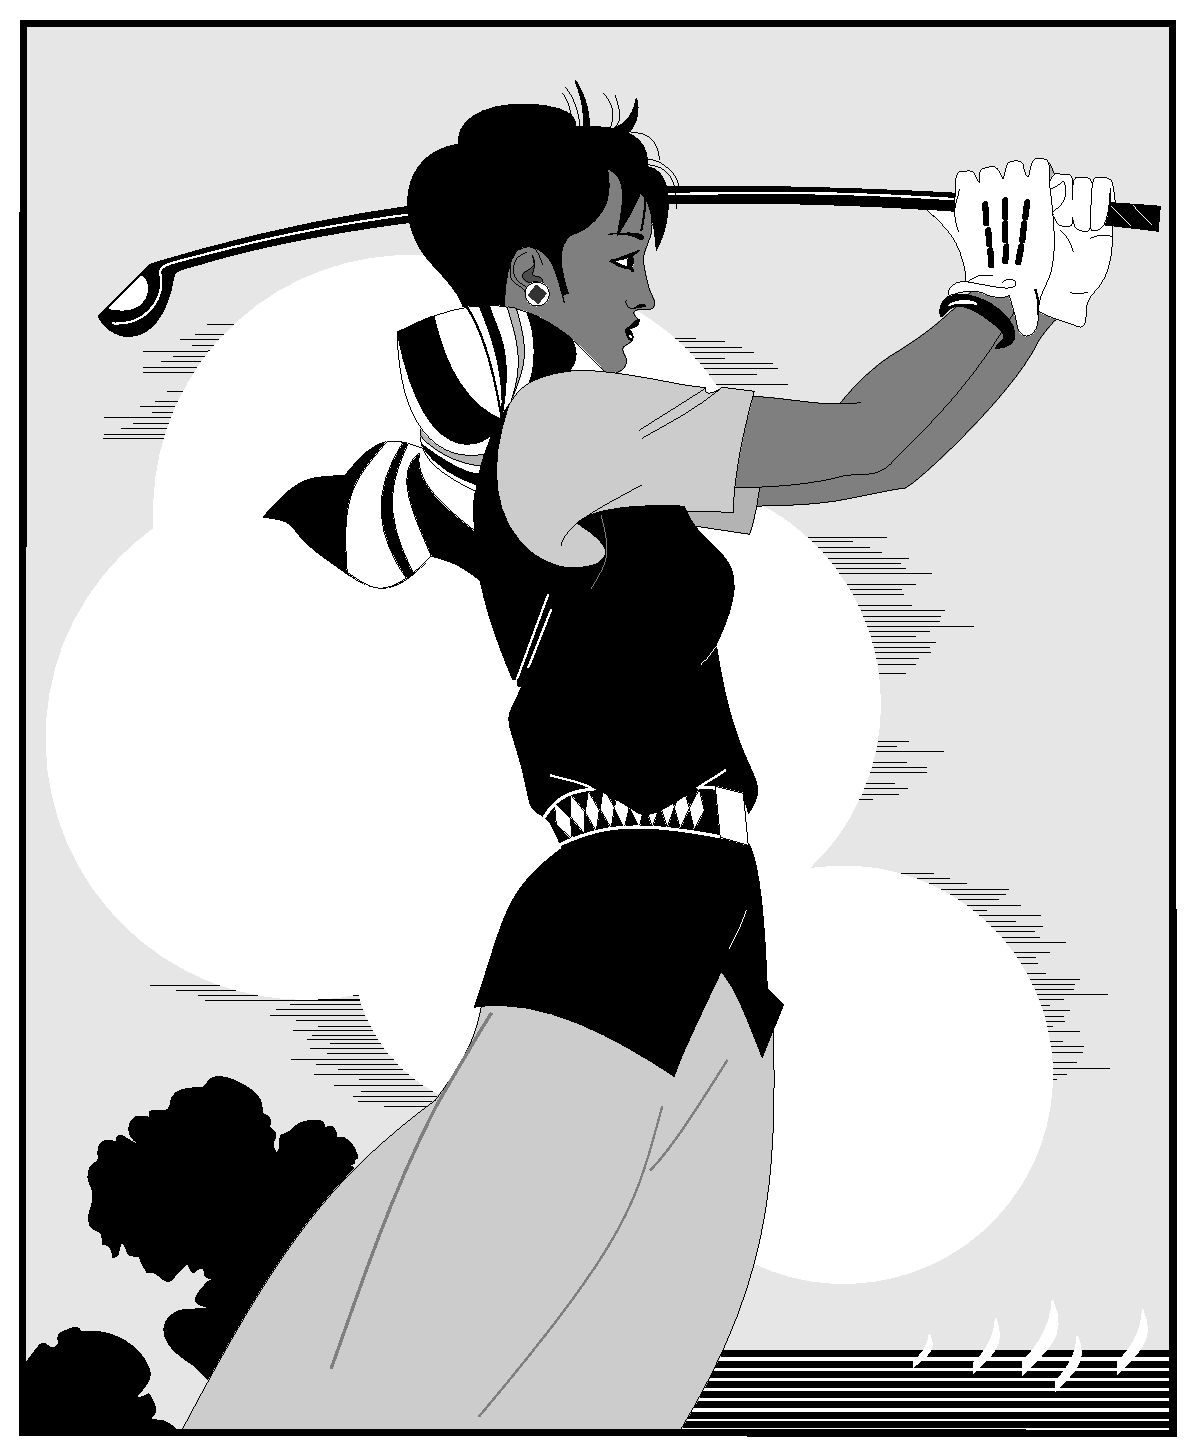
\includegraphics[width = 0.4\textwidth]{golfer}
	\bicaption[golfer1]{}{打高尔夫球球的人(博士论文双语题注)}{Fig.$\!$}{The person playing golf (Doctoral thesis)}
\end{figure}

每个图均应有图题(由图序和图名组成),图题不宜有标点符号,图名在图序之后空1个半
角字符排写。图序按章编排,如第1章第一个插图的图号为“图1-1”。图题置于图下,硕士论
文只用中文,博士论文用中、英两种文字,居中书写,中文在上,要求中文用宋体5号字,
英文用Times New Roman 5号字。有图注或其它说明时应置于图题之上。引用图应注明出处
,在图题右上角加引用文献号。图中若有分图时,分图题置于分图之下或图题之下,可以只
用中文书写,分图号用a)、b)等表示。图中各部分说明应采用中文(引用的外文图除外)或
数字符号,各项文字说明置于图题之上(有分图时,置于分图题之上)。图中文字用宋体、
Times New Roman字体,字号尽量采用5号字(当字数较多时可用小5号字,以清晰表达为原
则,但在一个插图内字号要统一)。同一图内使用文字应统一。图表中物理量、符号用斜体
。
\subsection{本硕论文题注}[Other picture example]
\begin{figure}[h]
	\centering
	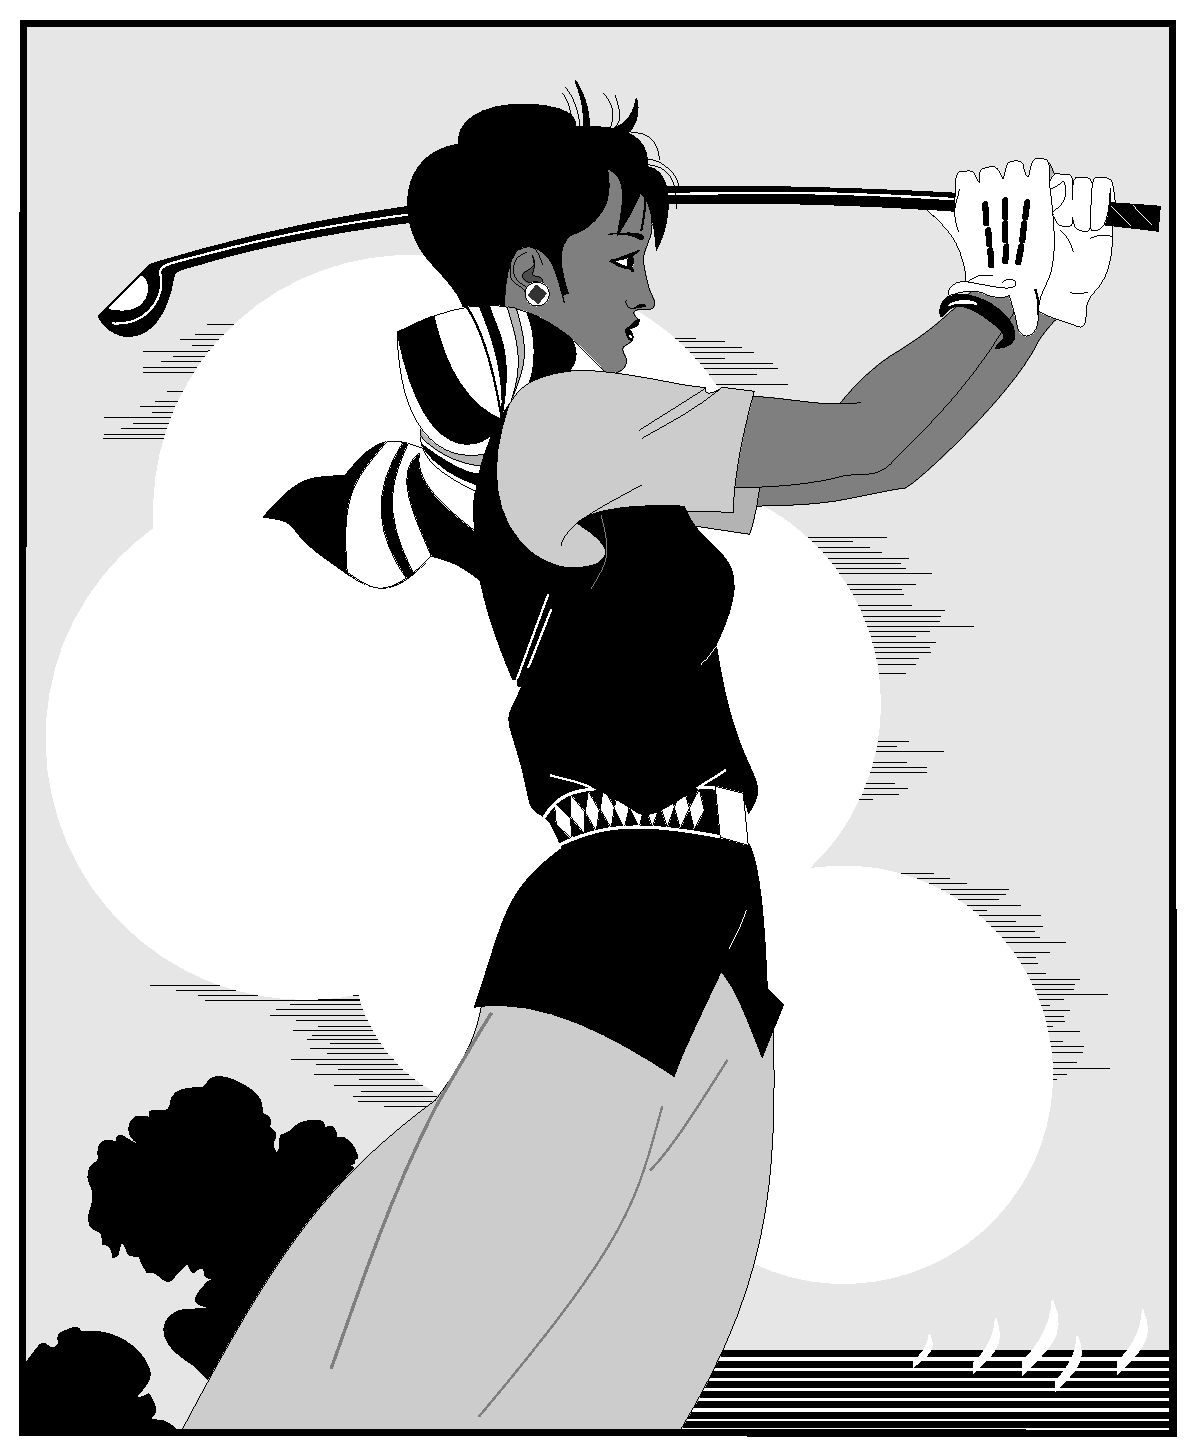
\includegraphics[width = 0.4\textwidth]{golfer}
	\caption{打高尔夫球的人,硕士论文要求只用汉语}
\end{figure}

\subsection{并排图和子图}[Abreast-picture and Sub-picture example]
\subsubsection{并排图}[Abreast-picture example]

使用并排图时,需要注意对齐方式。默认情况是中部对齐。这里给出中部对齐、顶部对齐
、图片底部对齐三种常见方式。其中,底部对齐方式有一个很巧妙的方式,将长度比较小
的图放在左面即可。

\begin{figure}[htbp]
	\centering
	\begin{minipage}{0.4\textwidth}
		\centering
		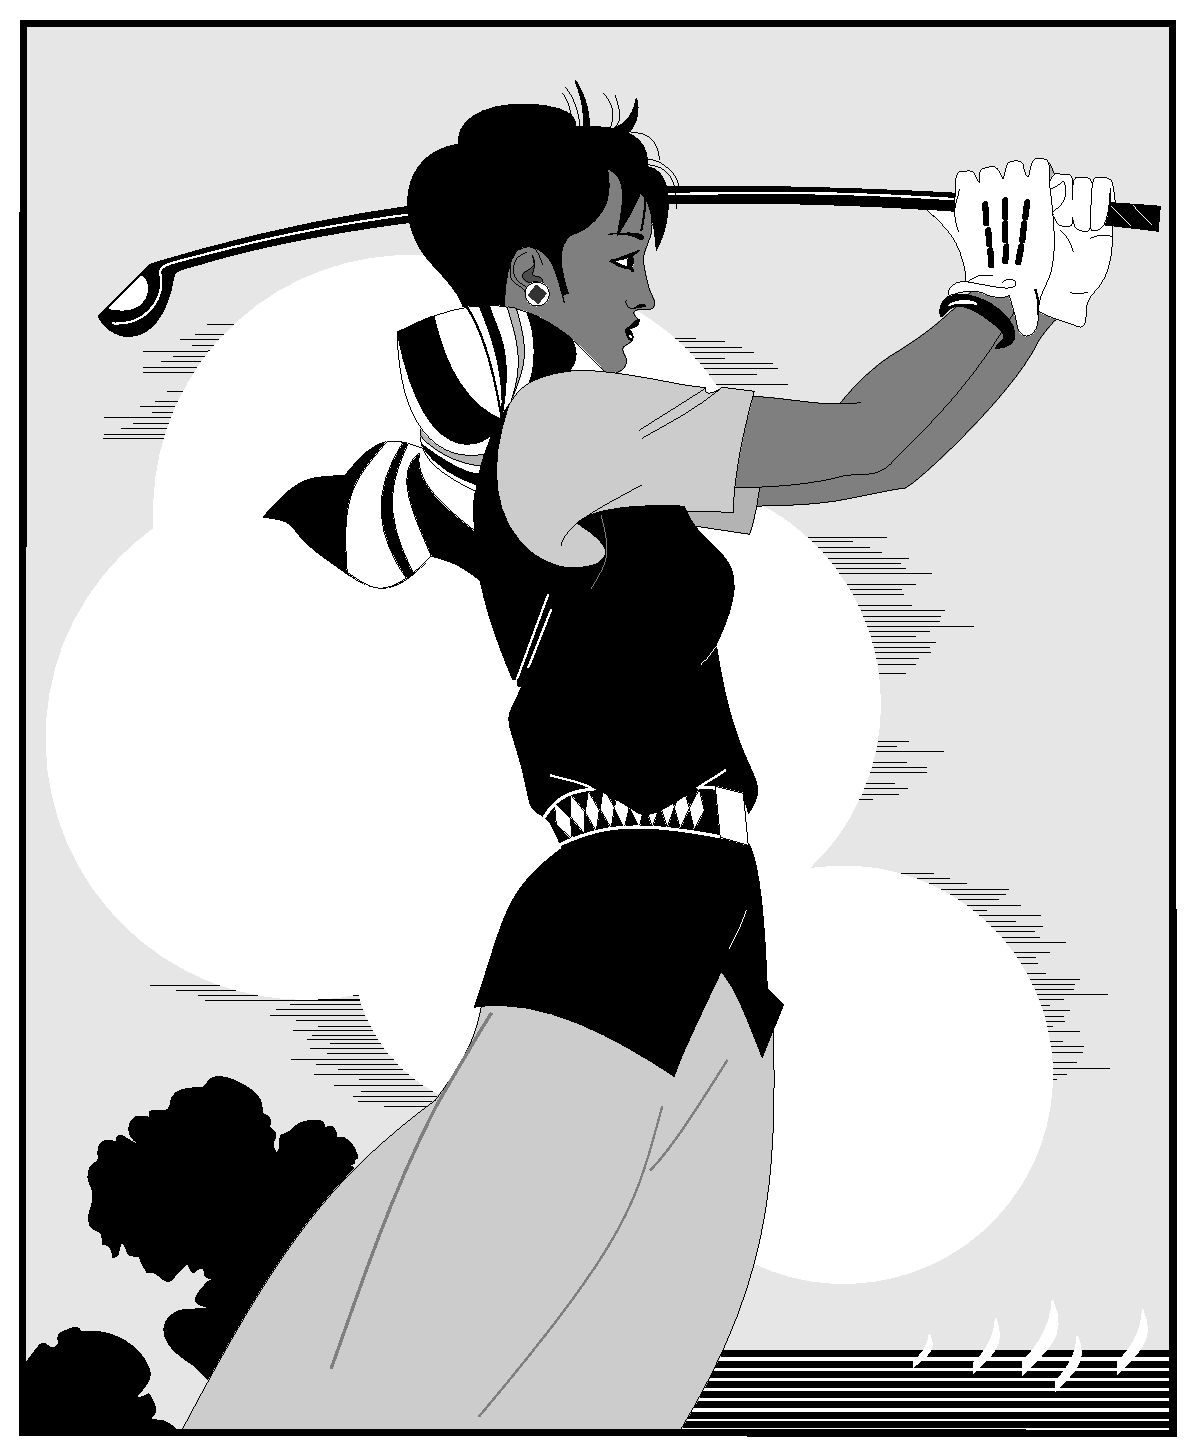
\includegraphics[width=\textwidth]{golfer}
		\bicaption[golfer2]{}{打高尔夫球的人}{Fig.$\!$}{The person playing golf}
	\end{minipage}
	\centering
	\begin{minipage}{0.4\textwidth}
		\centering
		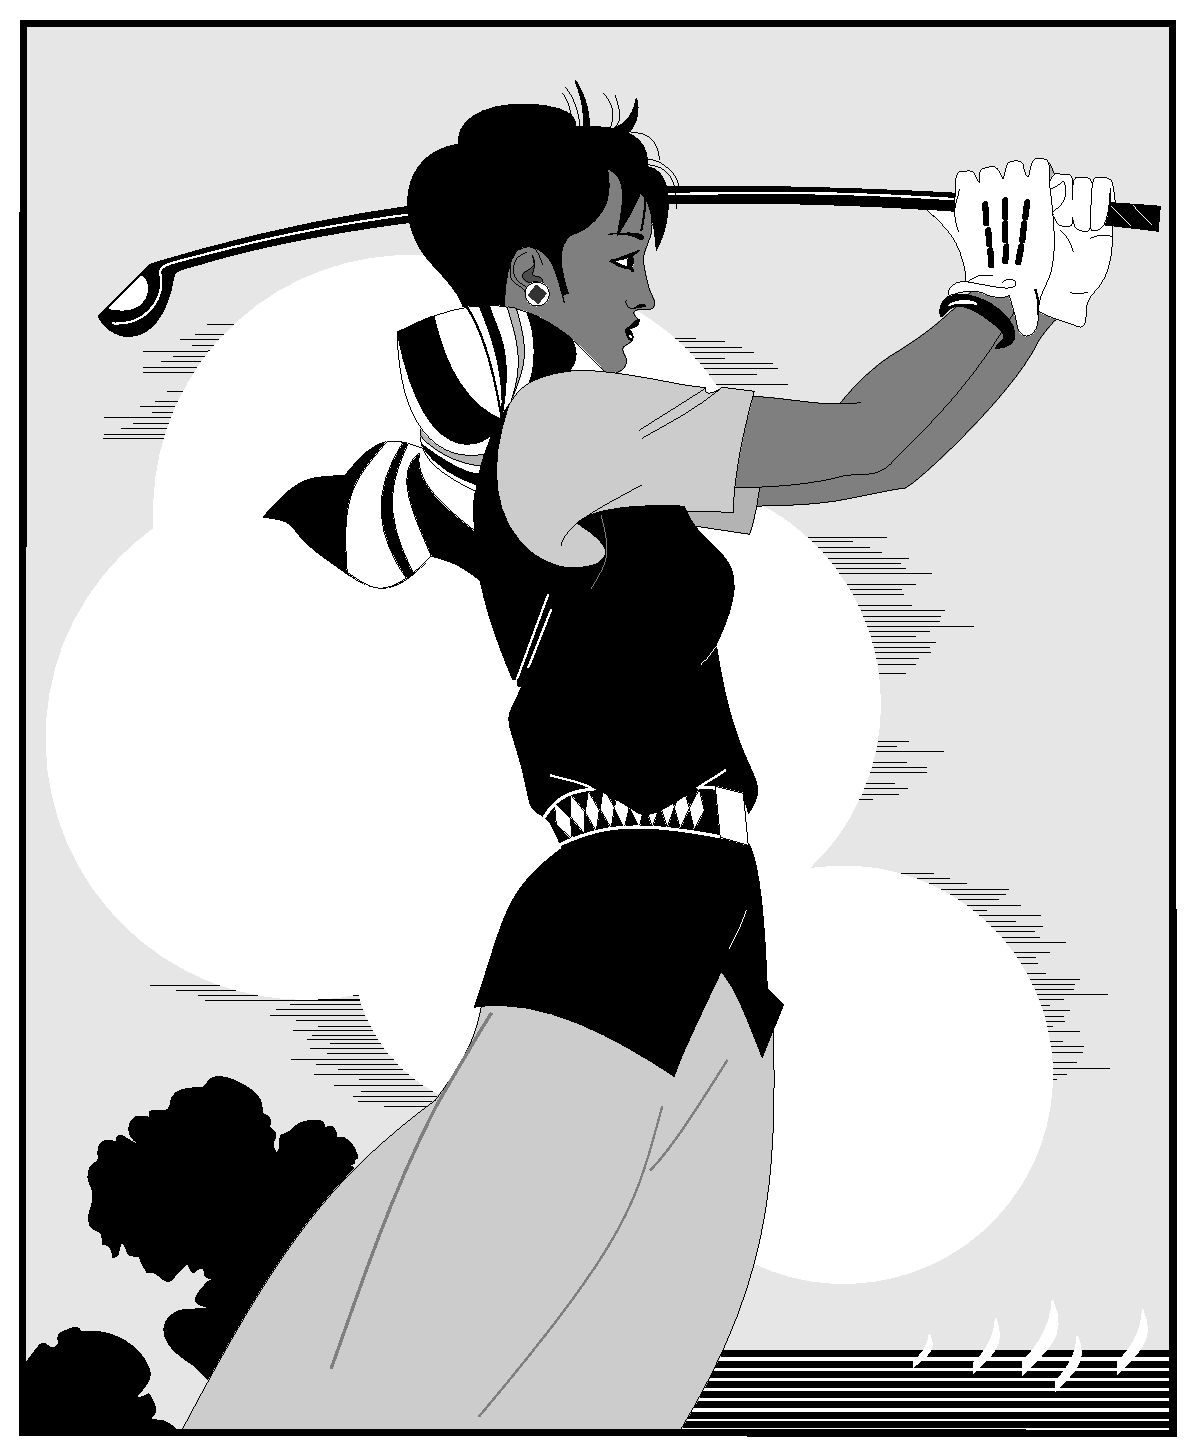
\includegraphics[width=\textwidth]{golfer}
		\bicaption[golfer3]{}{打高尔夫球的人。注意,这里默认居中}{Fig.$\!$}{The person playing golf. Please note that, it is vertically center aligned by default.}
	\end{minipage}
\end{figure}

\begin{figure}[htbp]
	\centering
	\begin{minipage}[t]{0.4\textwidth}
		\centering
		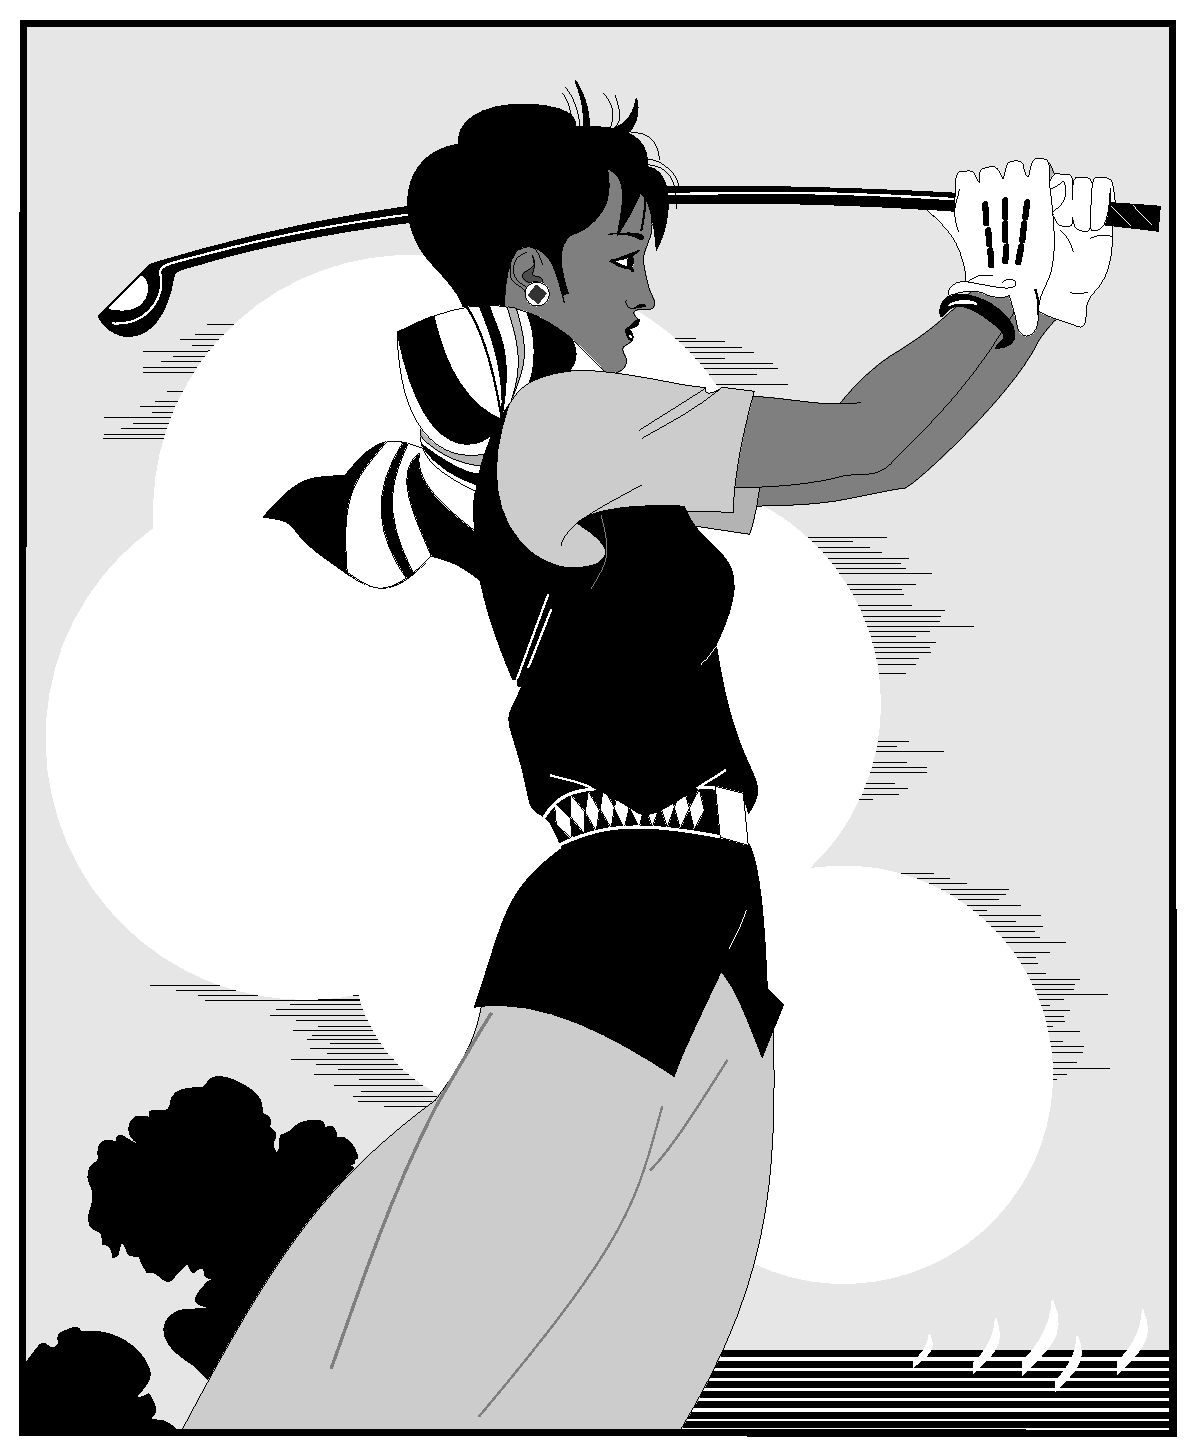
\includegraphics[width=\textwidth]{golfer}
		\bicaption[golfer5]{}{打高尔夫球的人}{Fig.$\!$}{The person playing golf}
	\end{minipage}
	\centering
	\begin{minipage}[t]{0.4\textwidth}
		\centering
		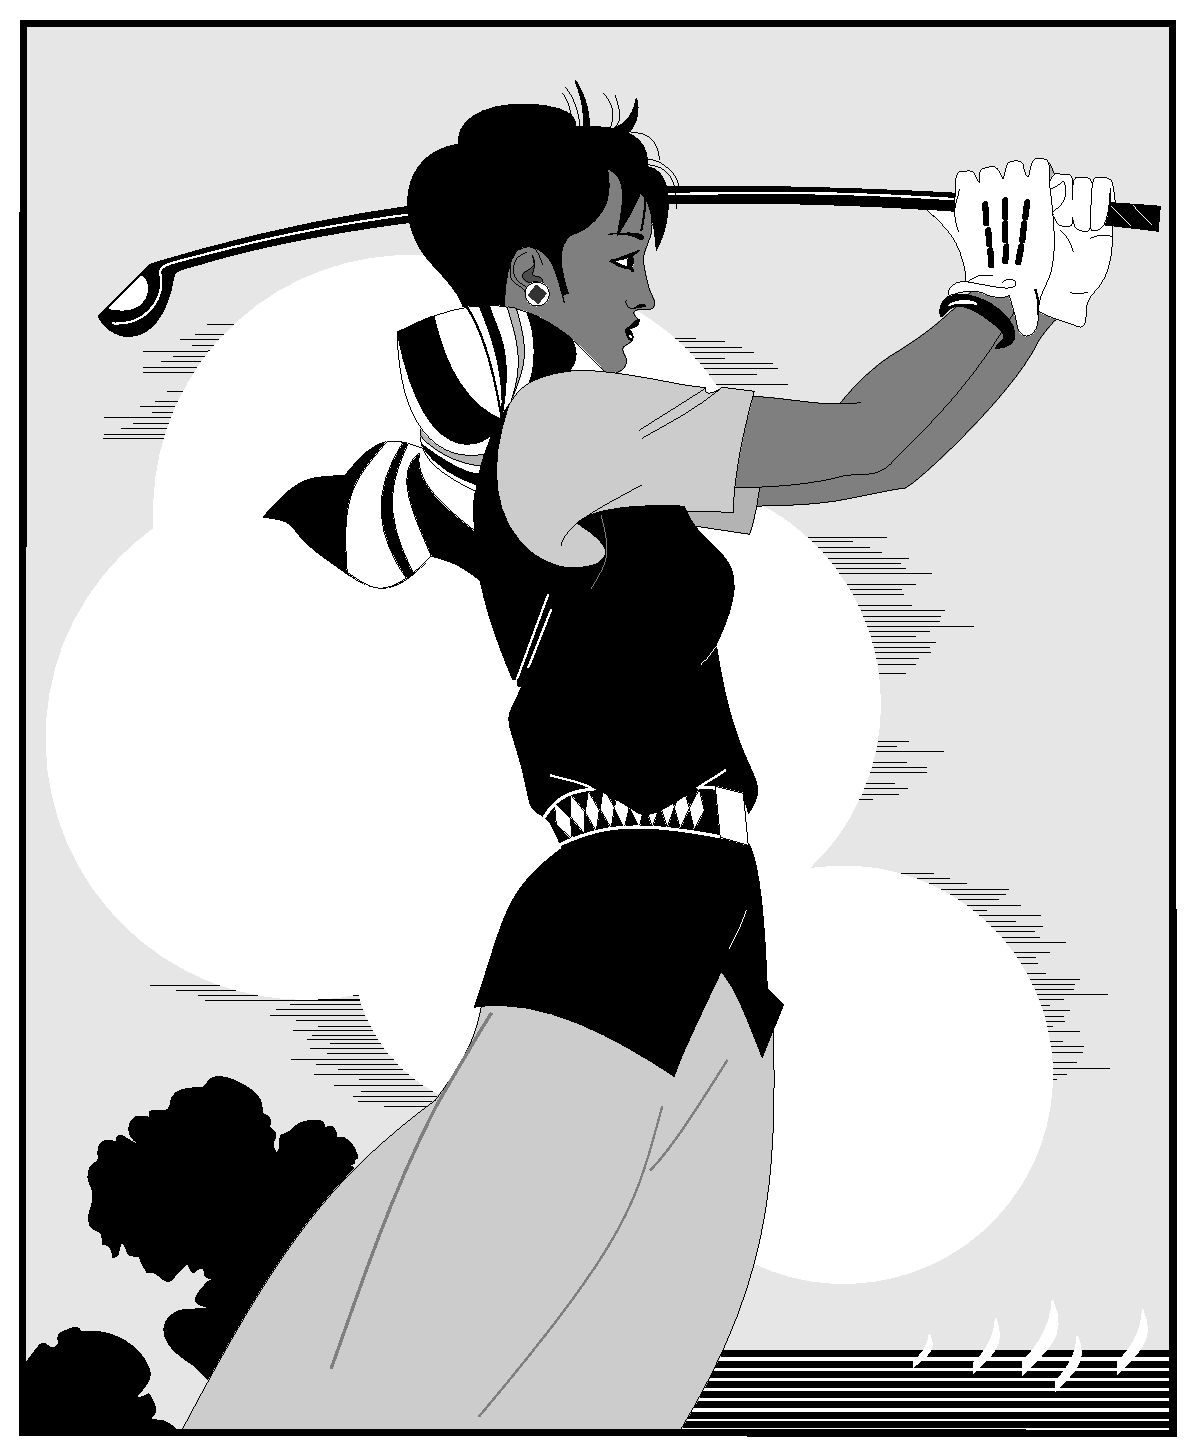
\includegraphics[width=\textwidth]{golfer}
		\bicaption[golfer8]{}{打高尔夫球的人。注意,此图是顶部对齐}{Fig.$\!$}{The person playing golf. Please note that, it is vertically top aligned.}
	\end{minipage}
\end{figure}

\begin{figure}[htbp]
	\centering
	\begin{minipage}[t]{0.4\textwidth}
		\centering
		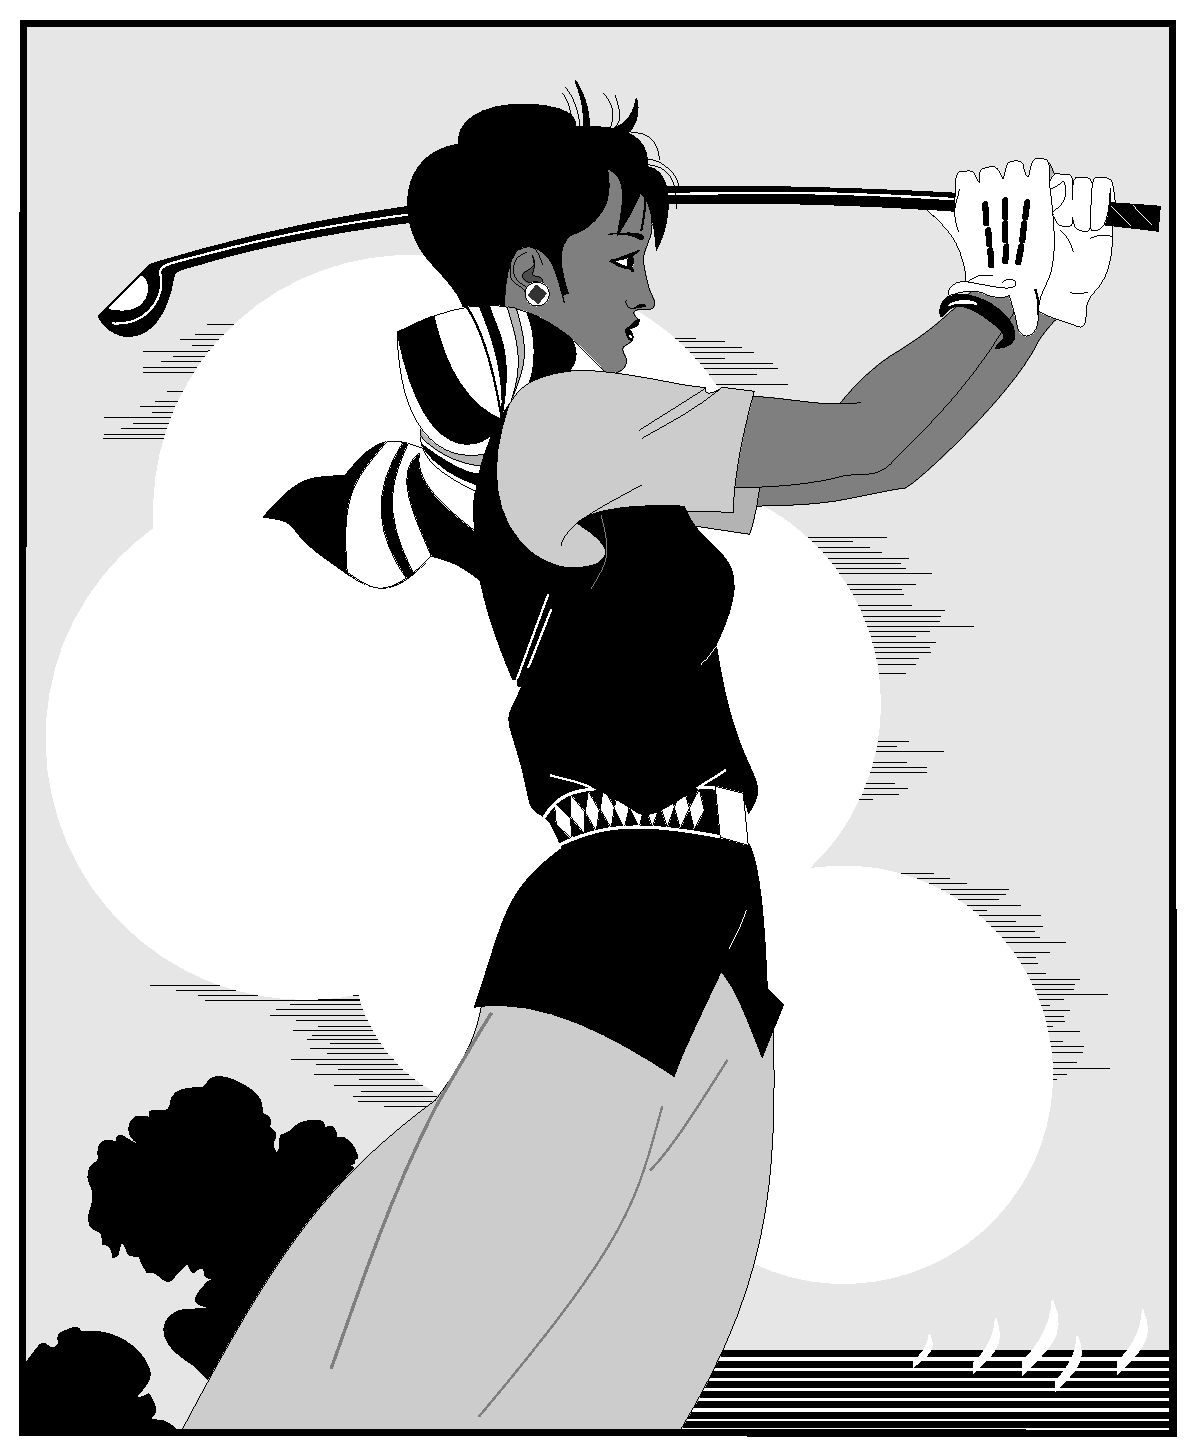
\includegraphics[width=\textwidth,height=\textwidth]{golfer}
		\bicaption[golfer9]{}{打高尔夫球的人。注意,此图对齐方式是图片底部对齐}{Fig.$\!$}{The person playing golf. Please note that, it is vertically bottom aligned for figure.}
	\end{minipage}
	\centering
	\begin{minipage}[t]{0.4\textwidth}
		\centering
		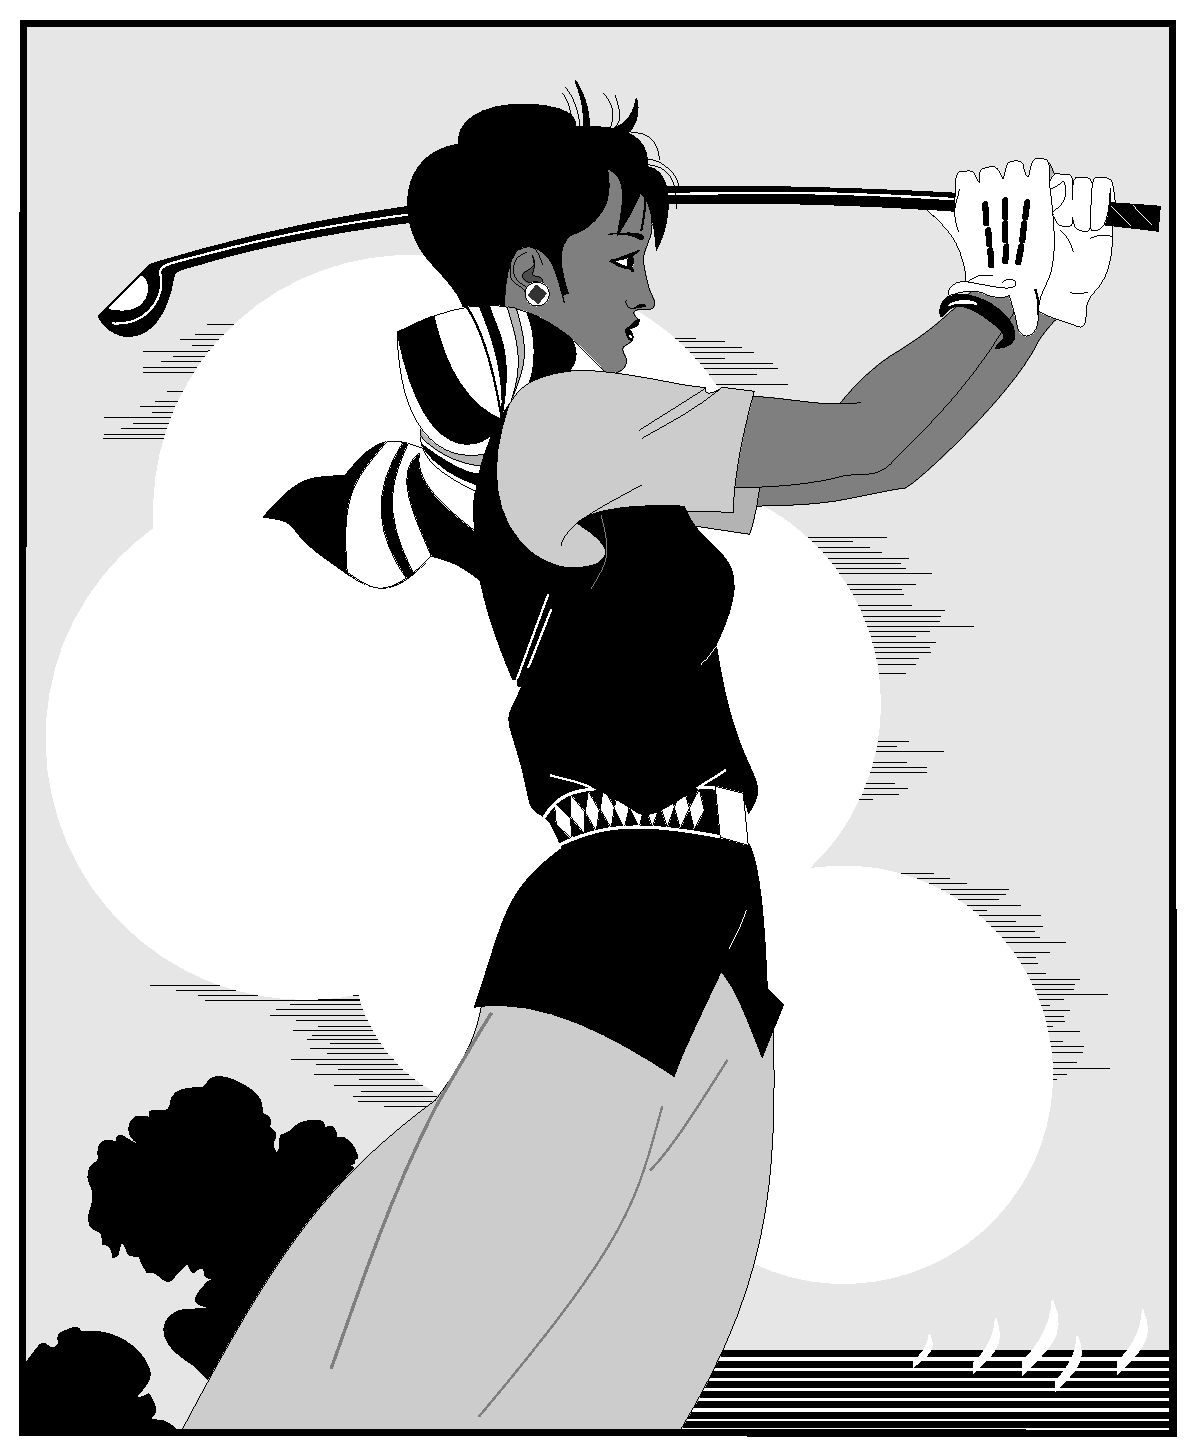
\includegraphics[width=\textwidth]{golfer}
		\bicaption[golfer6]{}{打高尔夫球的人}{Fig.$\!$}{The person playing golf}
	\end{minipage}
\end{figure}

\subsubsection{子图}[Sub-picture example]
注意:子图题注也可以只用中文。规范规定“分图题置于分图之下或图题之下”,但没有给出具体的格式要求。
没有要求的另外一个说法就是“无论什么格式都不对”。
所以只有在一个图中有标注“a),b)”,无法使用\cs{subfigure}的情况下,使用最后一个图例中的格式设置方法,否则不要使用。
为了应对“无论什么格式都不对”,这个子图图题使用“minipage”和“description”环境,宽度,对齐方式可以按照个人喜好自由设置,是否使用双语子图图题也可以自由设置。

\begin{figure}[!h]
	\setlength{\subfigcapskip}{-1bp}
	\centering
	\begin{minipage}{\textwidth}
		\centering
		\subfigure{\label{golfer41}}\addtocounter{subfigure}{-2}
		\subfigure[The person playing golf]{\subfigure[打高尔夫球的人~1]{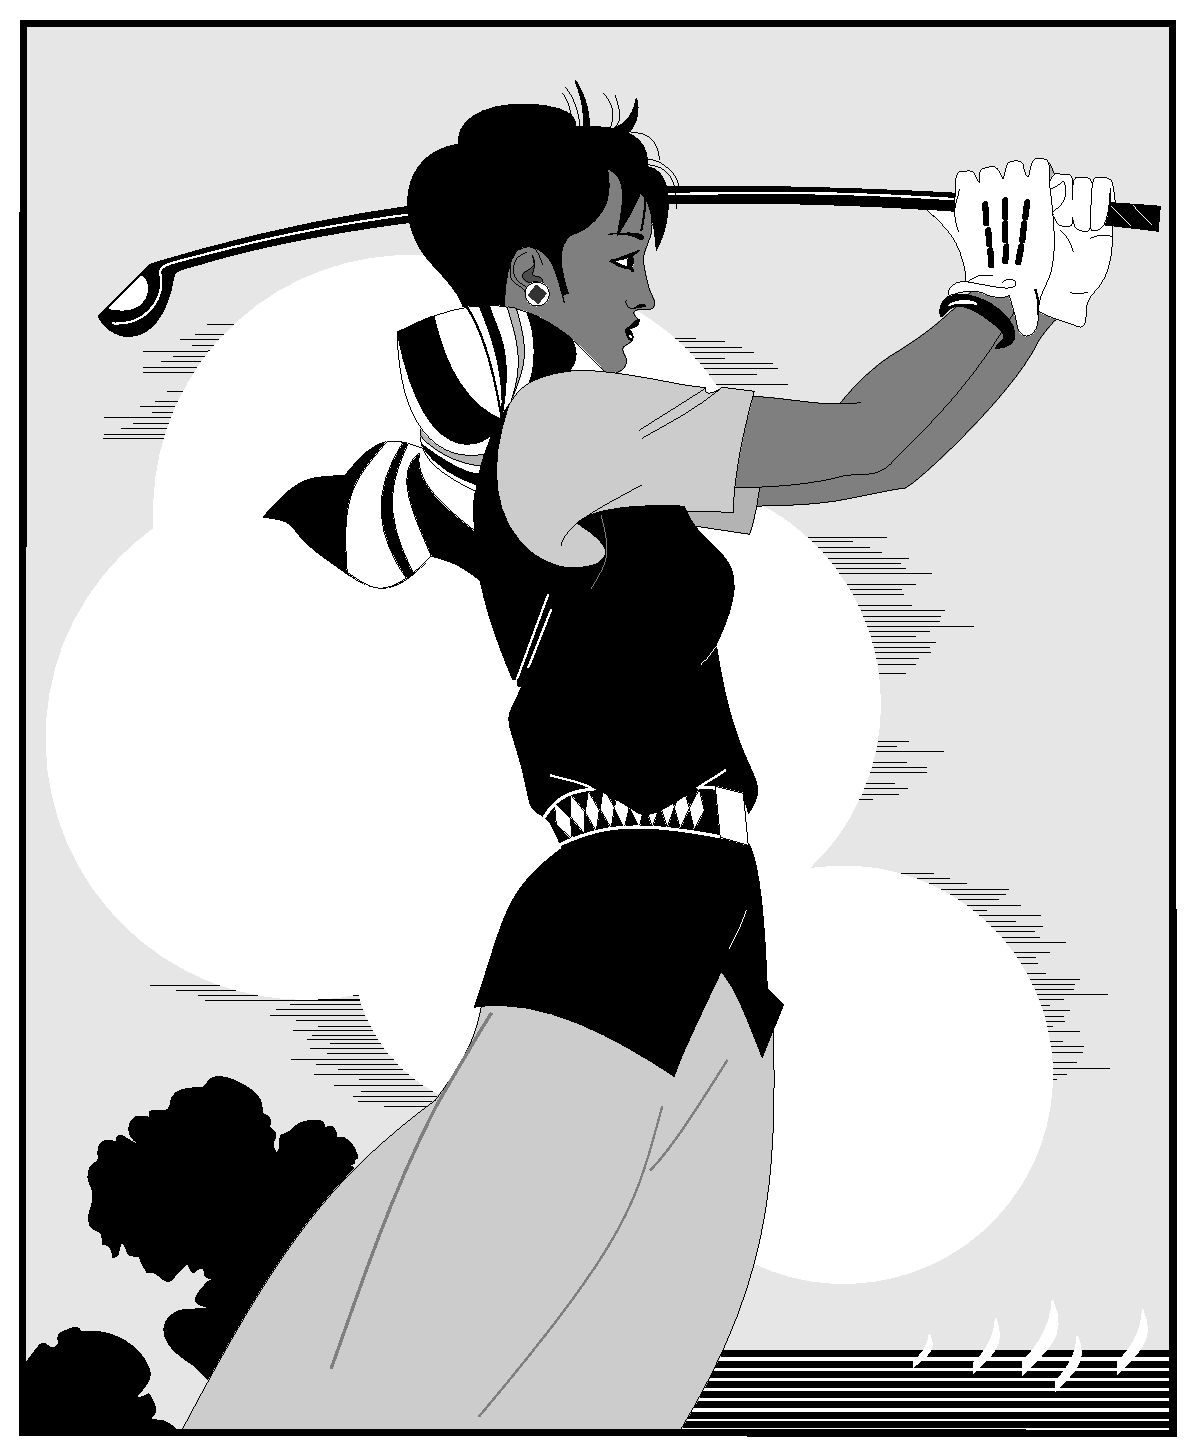
\includegraphics[width=0.4\textwidth]{golfer}}}
		\hspace{2em}
		\subfigure{\label{golfer42}}\addtocounter{subfigure}{-2}
		\subfigure[The person playing golf]{\subfigure[打高尔夫球的人~2]{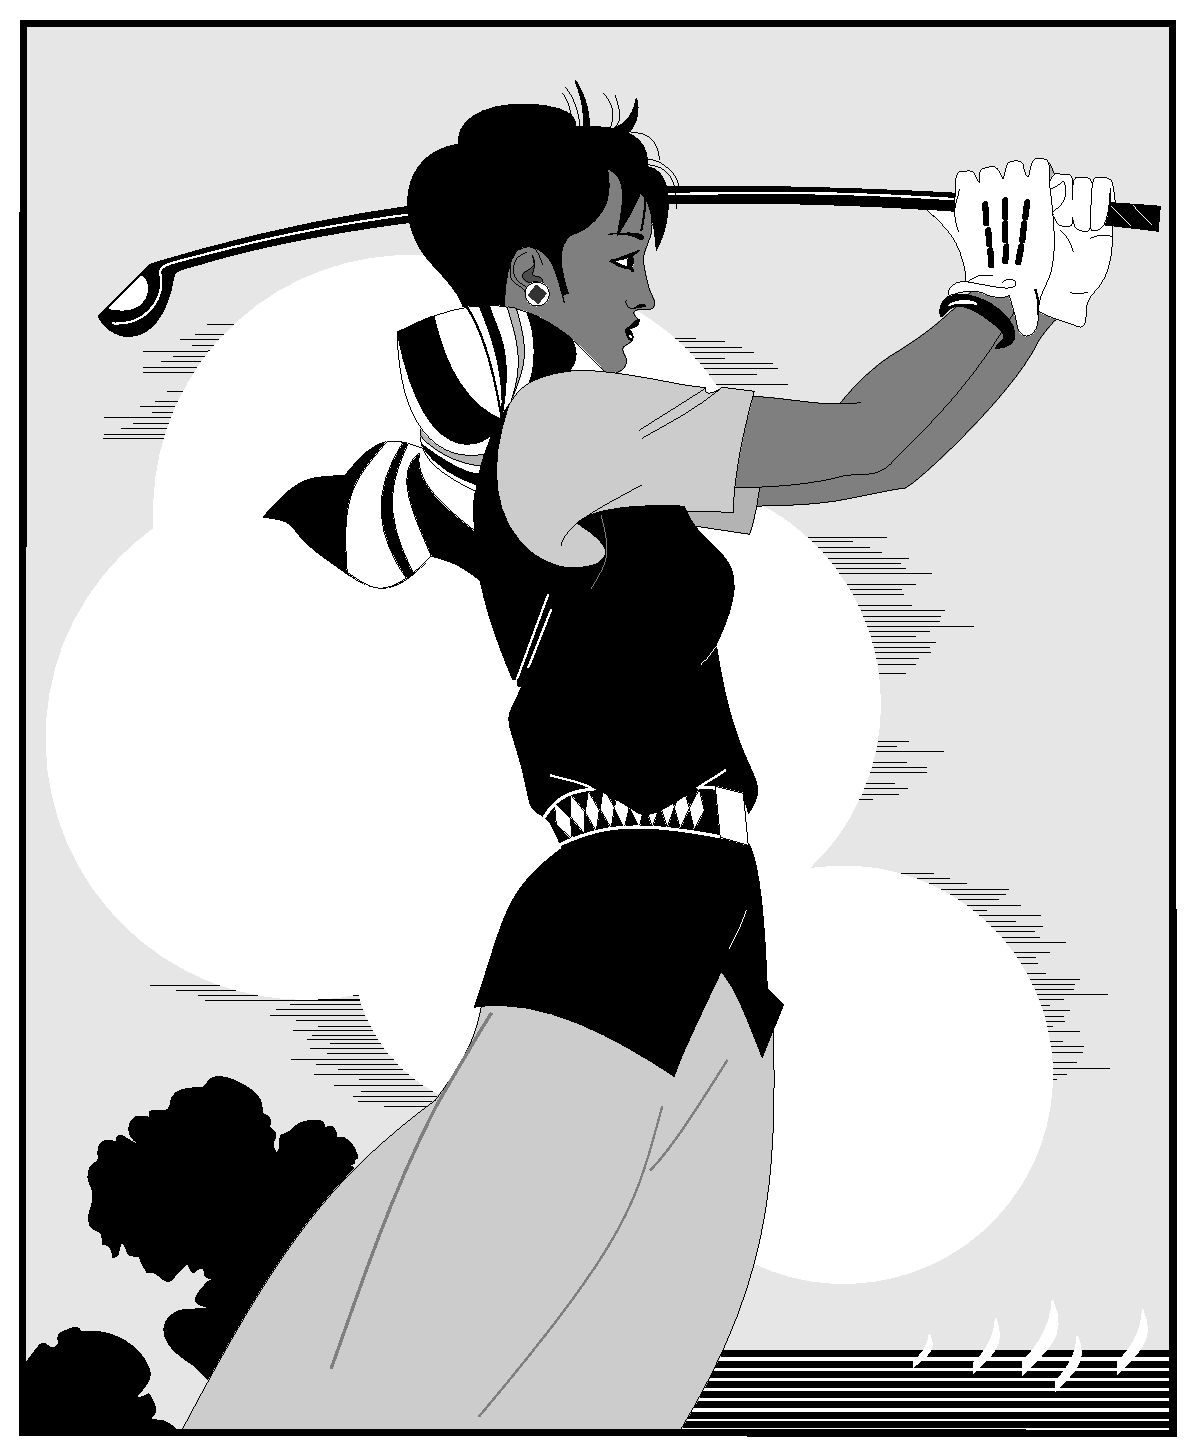
\includegraphics[width=0.4\textwidth]{golfer}}}
	\end{minipage}
	\centering
	\begin{minipage}{\textwidth}
		\centering
		\subfigure{\label{golfer43}}\addtocounter{subfigure}{-2}
		\subfigure[The person playing golf]{\subfigure[打高尔夫球的人~3]{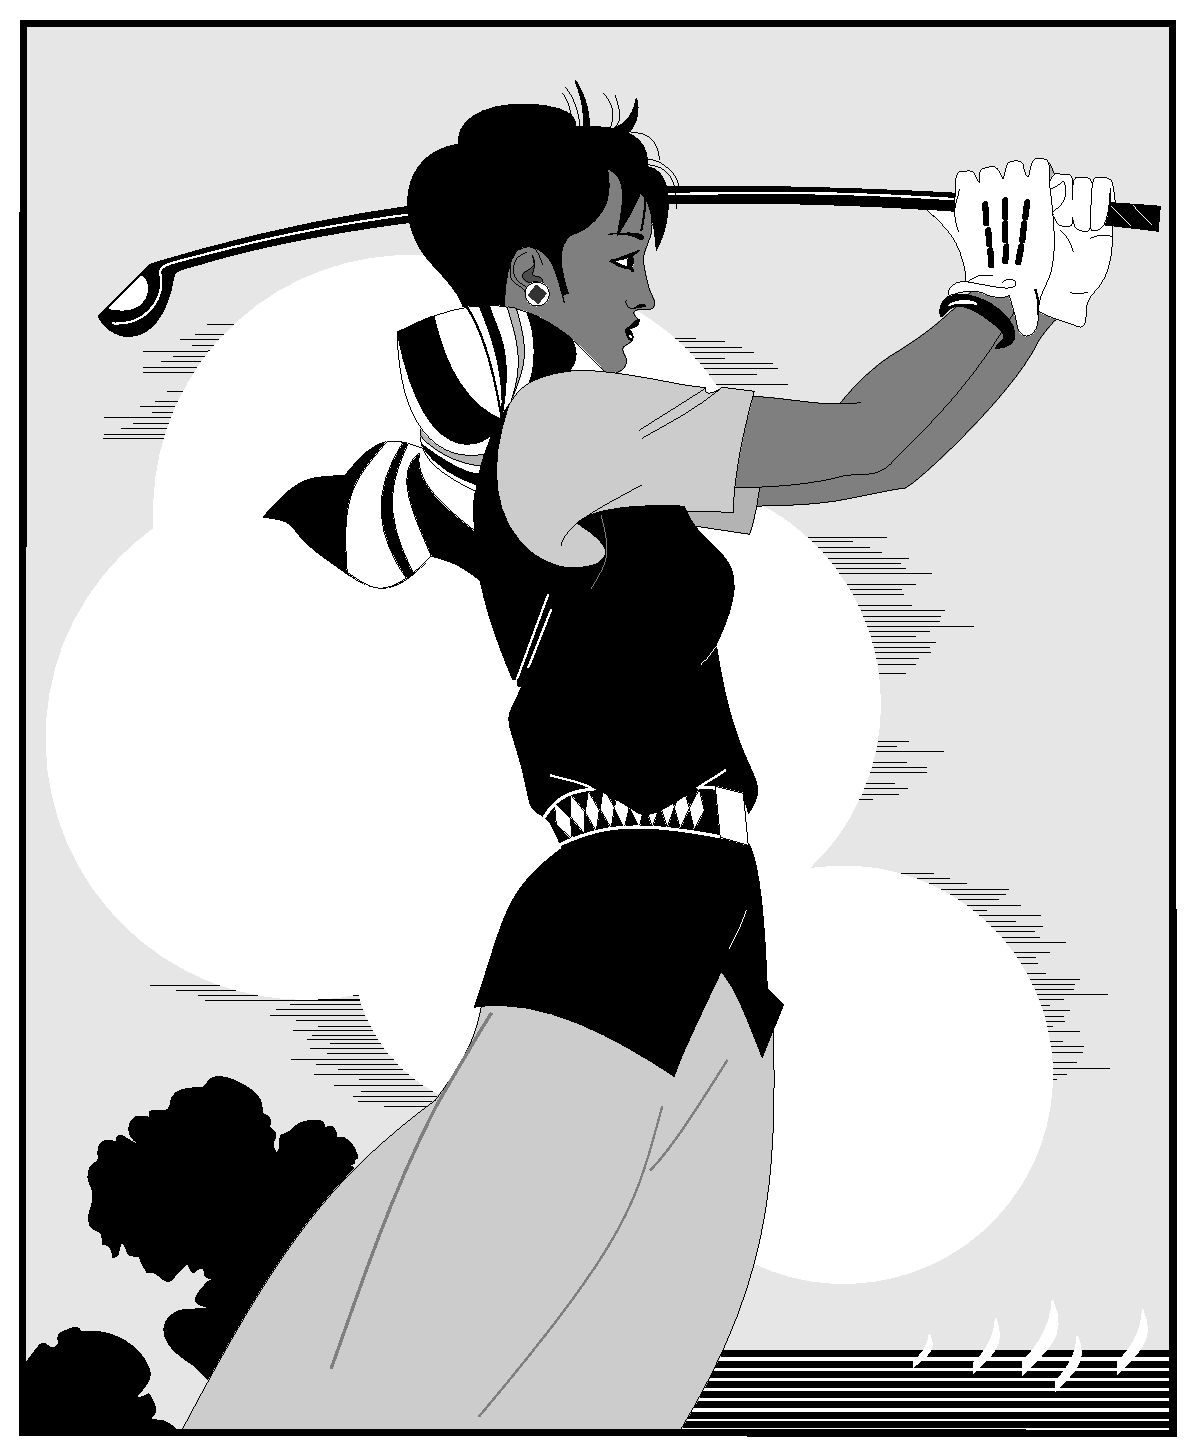
\includegraphics[width=0.4\textwidth]{golfer}}}
		\hspace{2em}
		\subfigure{\label{golfer44}}\addtocounter{subfigure}{-2}
		\subfigure[The person playing golf. Here, 'hang indent' and 'center last line' are not stipulated in the regulation.]{\subfigure[打高尔夫球的人~4。注意,规范中没有明确规定要悬挂缩进、最后一行居中。]{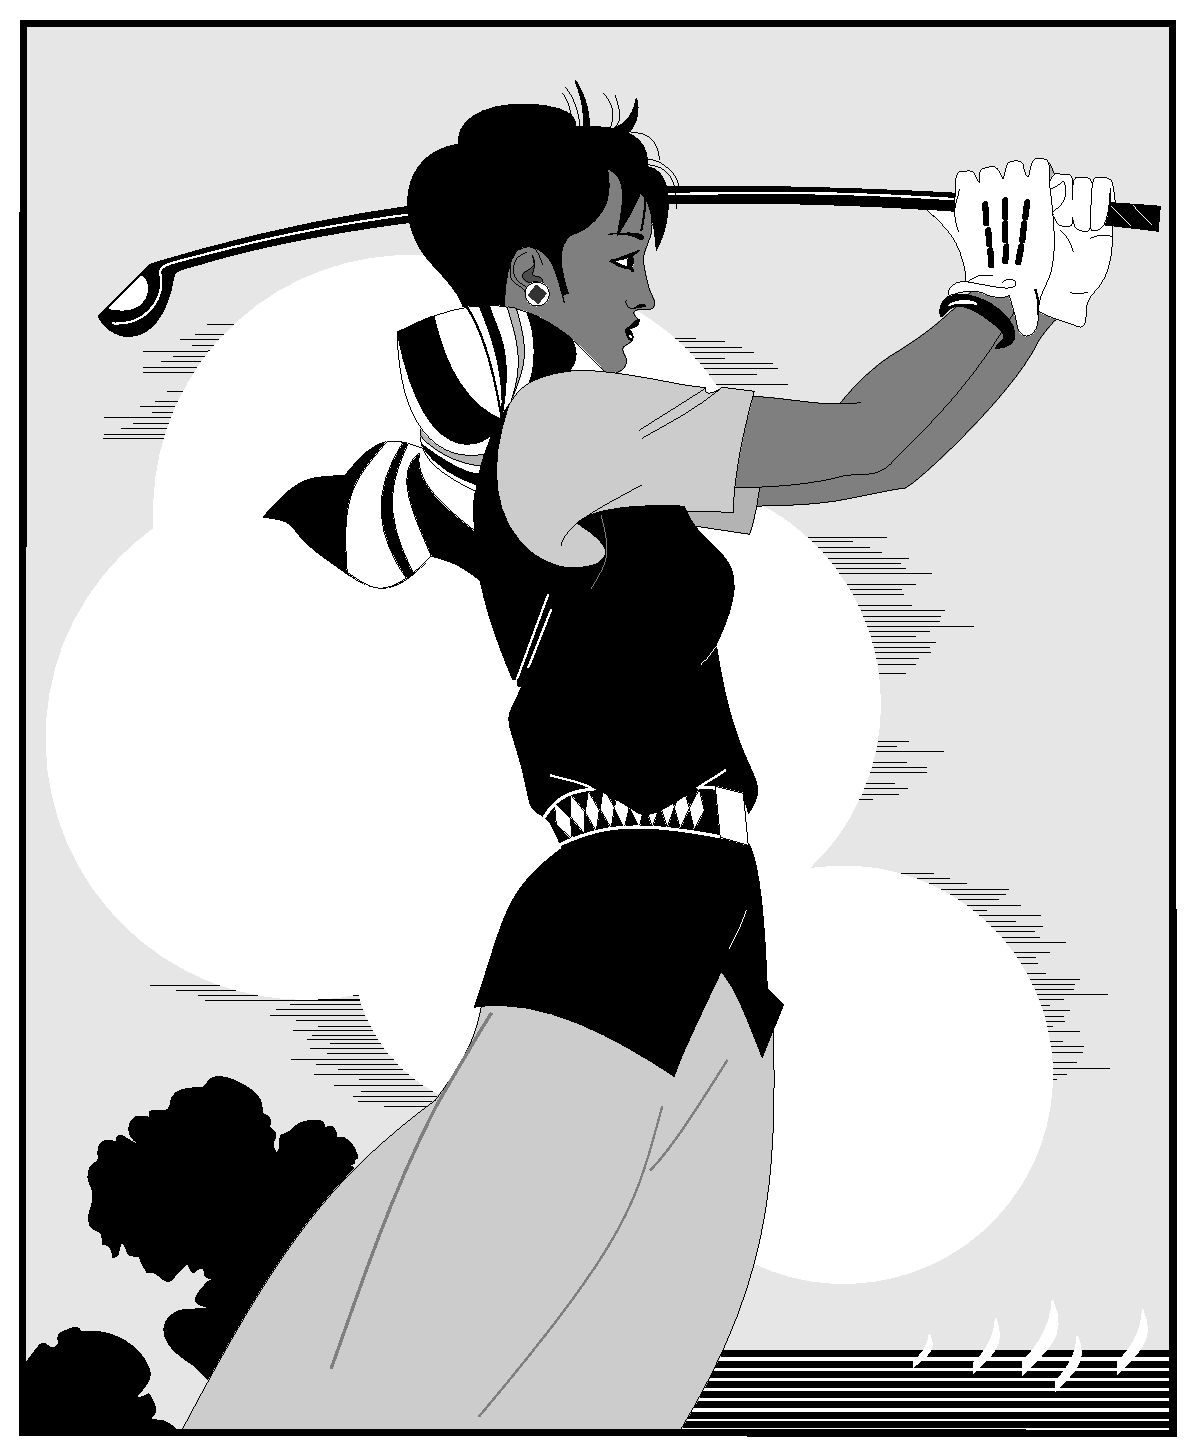
\includegraphics[width=0.4\textwidth]{golfer}}}
	\end{minipage}
	\vspace{0.2em}
	\bicaption[golfer4]{}{打高尔夫球的人}{Fig.$\!$}{The person playing gol}
\end{figure}

\begin{figure}[t]
	\centering
	\begin{minipage}{.7\linewidth}
		\setlength{\subfigcapskip}{-1bp}
		\centering
		\begin{minipage}{\textwidth}
			\centering
			\subfigure{\label{golfer45}}\addtocounter{subfigure}{-2}
			\subfigure[The person playing golf]{\subfigure[打高尔夫球的人~1]{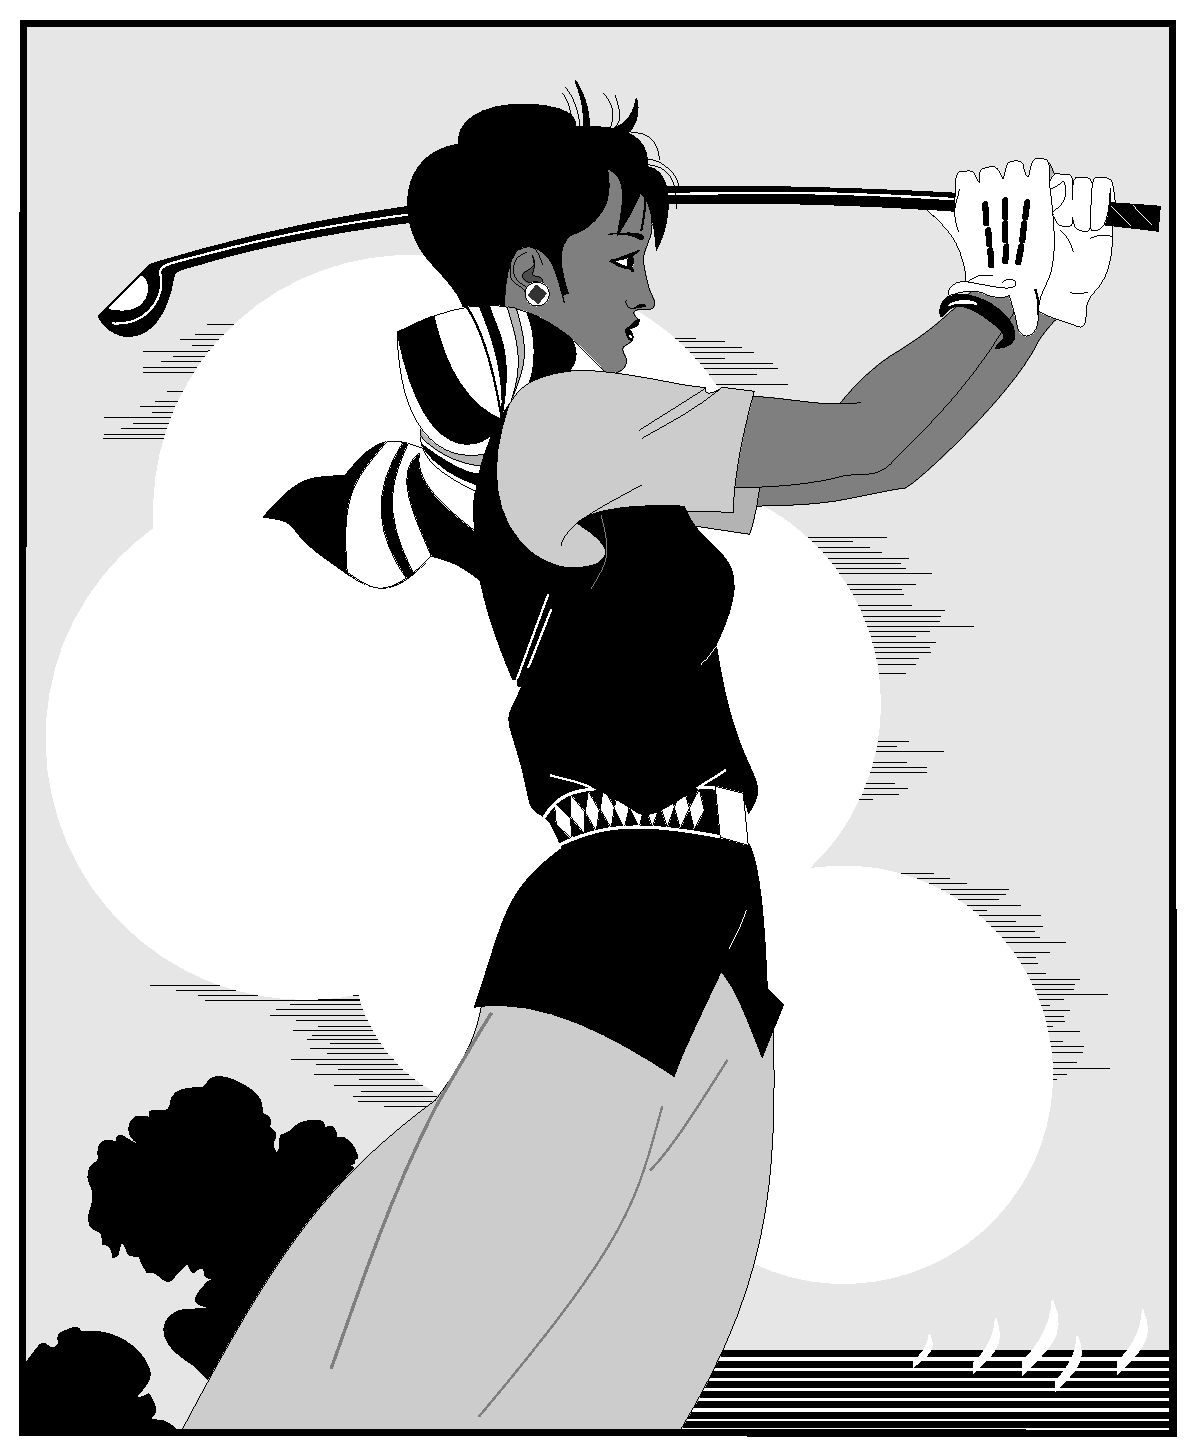
\includegraphics[width=0.4\textwidth]{golfer}}}
			\hspace{4em}
			\subfigure{\label{golfer46}}\addtocounter{subfigure}{-2}
			\subfigure[The person playing golf]{\subfigure[打高尔夫球的人~2]{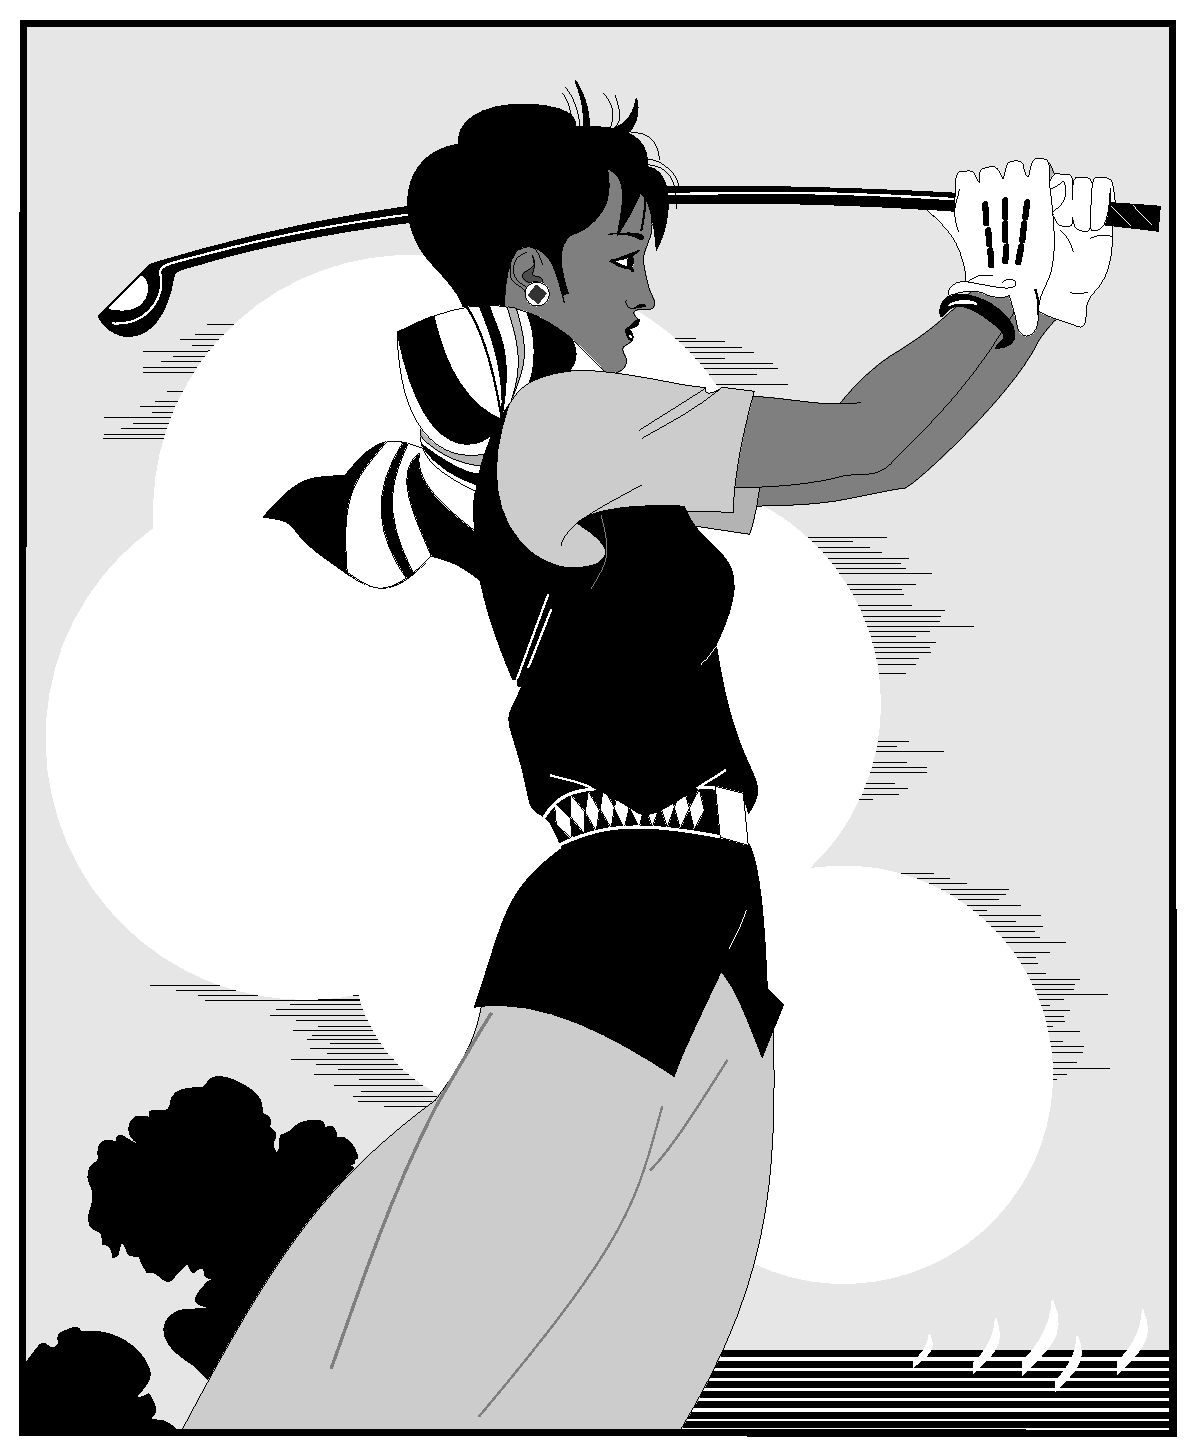
\includegraphics[width=0.4\textwidth]{golfer}}}
		\end{minipage}
		\vskip 0.2em
		\wuhao 注意:这里是中文图注添加位置(我工要求,图注在图题之上)。
		\vspace{0.2em}
		\bicaption[golfer47]{}{打高尔夫球的人。注意,此处我工有另外一处要求,子图图题可以位于主图题之下。但由于没有明确说明位于下方具体是什么格式,所以这里不给出举例。}{Fig.$\!$}{The person playing golf. Please note that, although it is appropriate to put subfigures' captions under this caption as stipulated in regulation, but its format is not clearly stated.}
	\end{minipage}
\end{figure}

\begin{figure}[t]
	\centering
	\begin{tikzpicture}
		\node[anchor=south west,inner sep=0] (image) at (0,0) {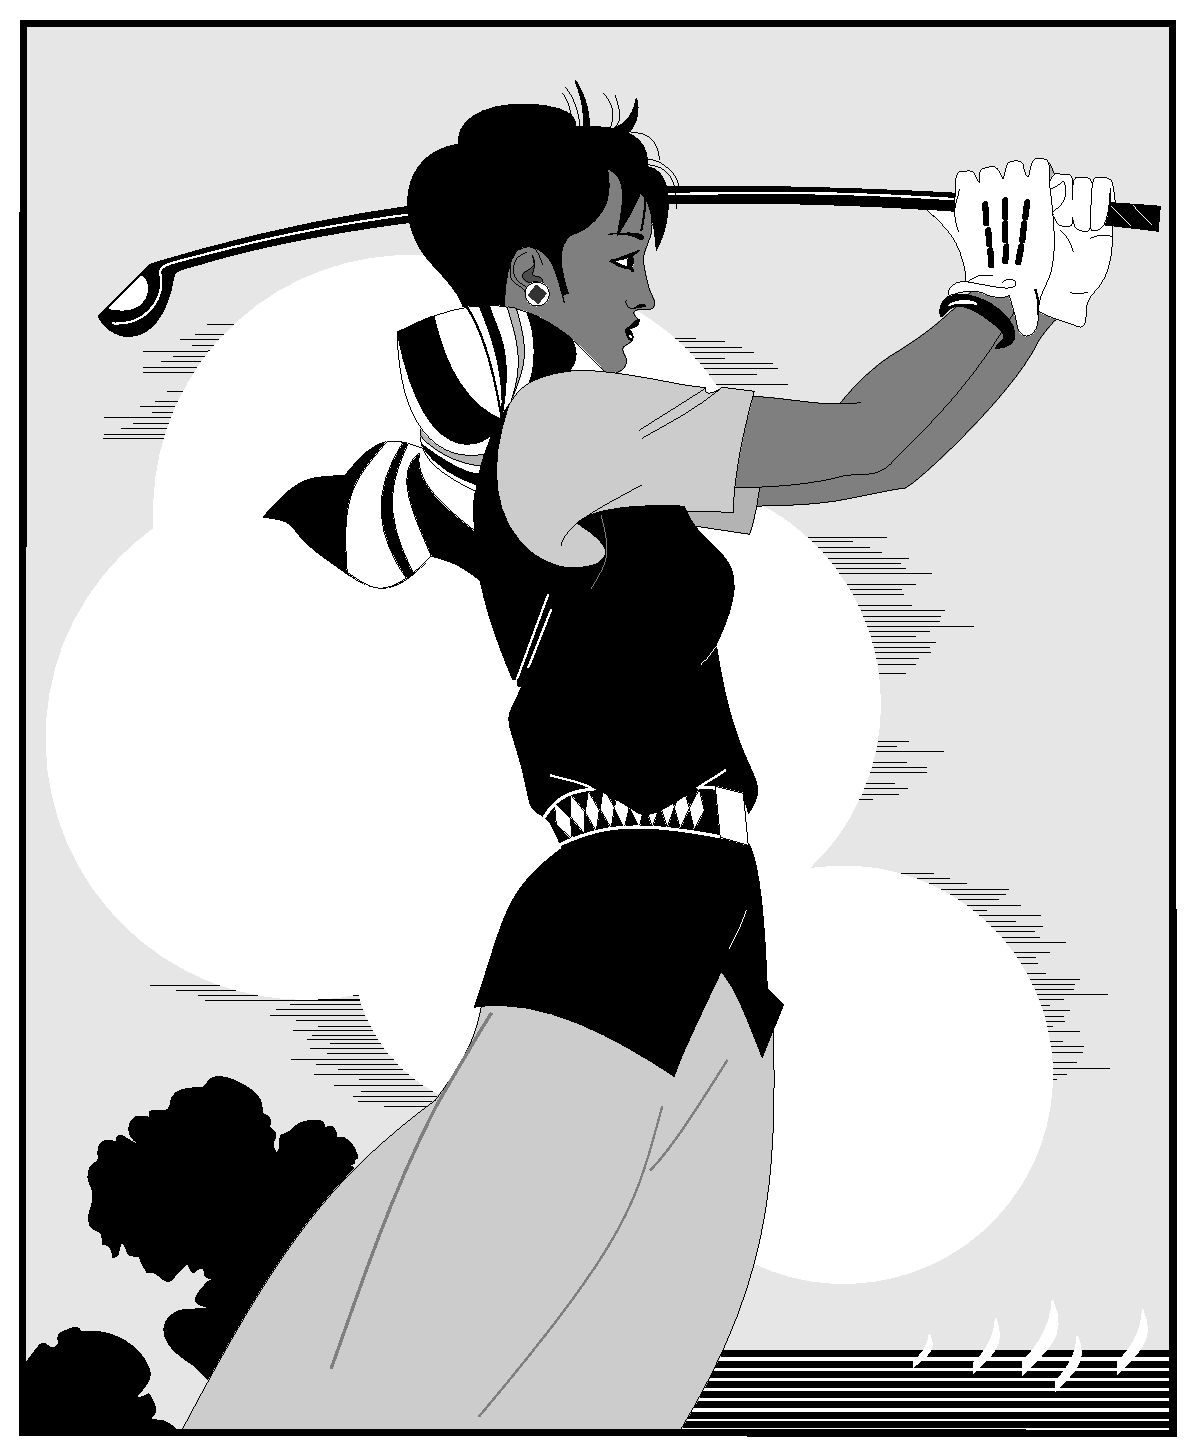
\includegraphics[width=0.3\textwidth]{golfer}};
		\begin{scope}[x={(image.south east)},y={(image.north west)}]
			\node at (0.3,0.5) {a)};
			\node at (0.8,0.2) {b)};
		\end{scope}
	\end{tikzpicture}
	\bicaption[golfer0]{}{打高尔夫球球的人(博士论文双语题注)}{Fig.$\!$}{The person playing golf (Doctoral thesis)}
	\vskip -0.4em
	\hspace{2em}
	\begin{minipage}[t]{0.3\textwidth}
		\wuhao \setlist[description]{font=\normalfont}
		\begin{description}
			\item[(a)]子图图题
		\end{description}
	\end{minipage}
	\hspace{2em}
	\begin{minipage}[t]{0.3\textwidth}
		\wuhao \setlist[description]{font=\normalfont}
		\begin{description}
			\item[(b)]子图图题
			\item[(b)]Subfigure caption
		\end{description}
	\end{minipage}
\end{figure}


\begin{figure}[!h]
	\centering
	\begin{sideways}
		\begin{minipage}{\textheight}
			\centering
			\fbox{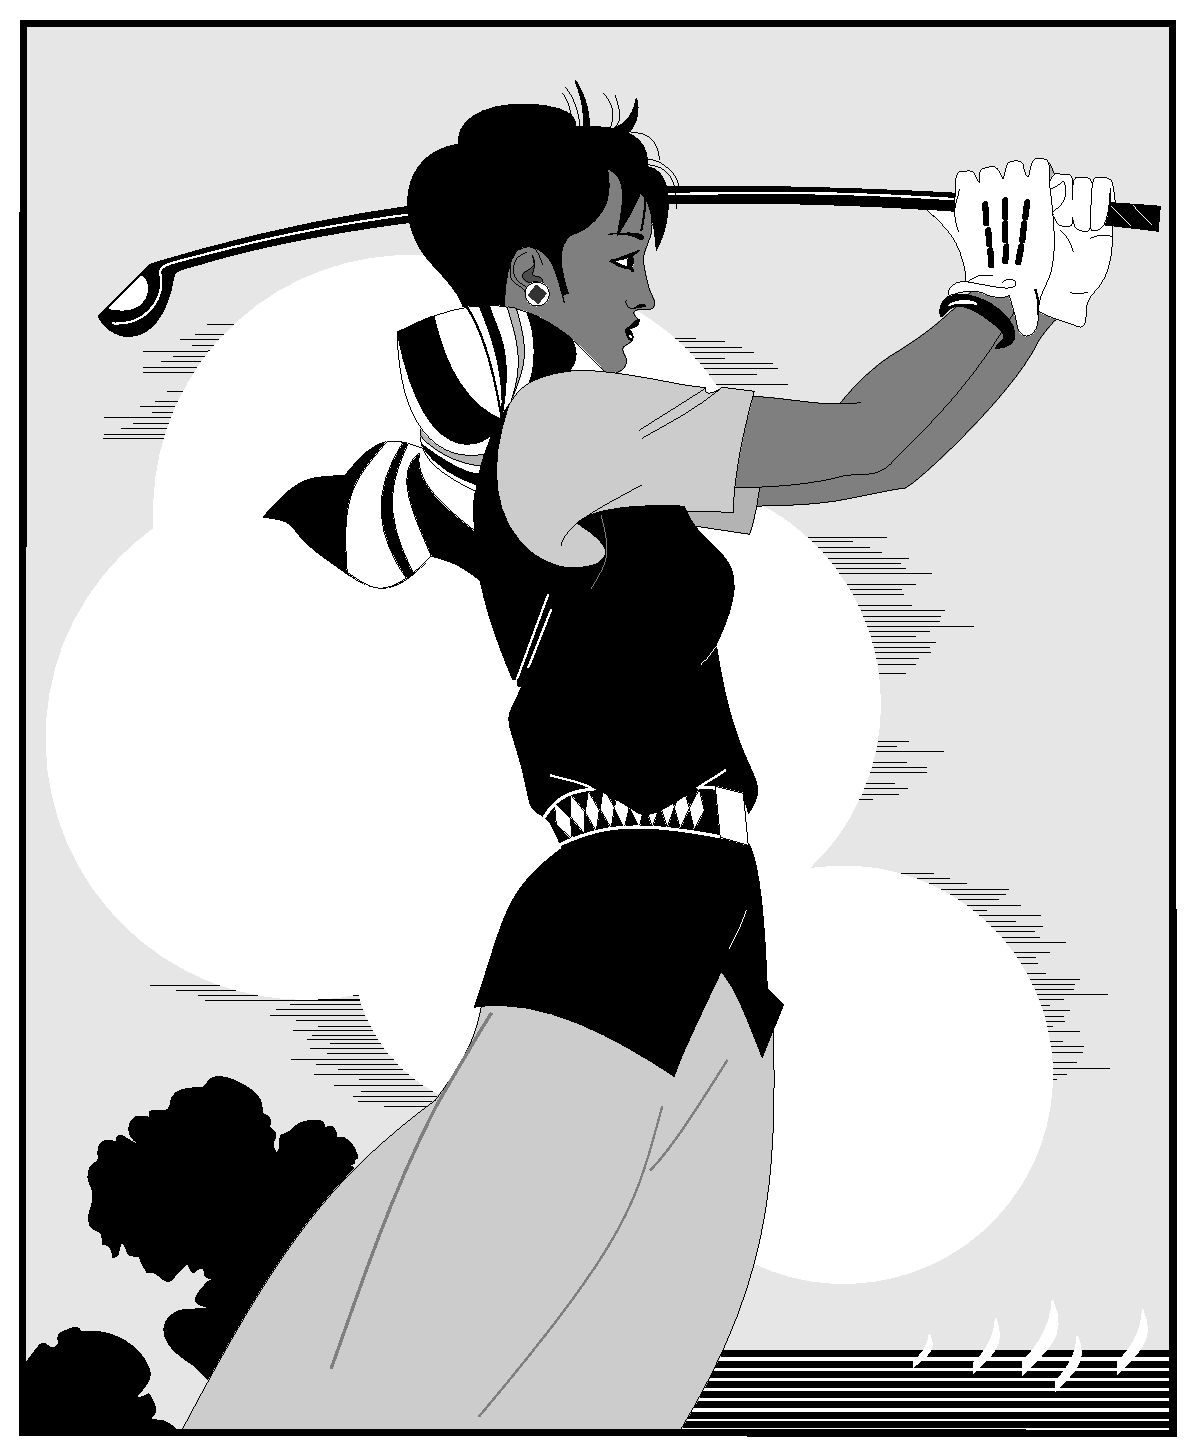
\includegraphics[width=0.2\textwidth]{golfer}}
			\fbox{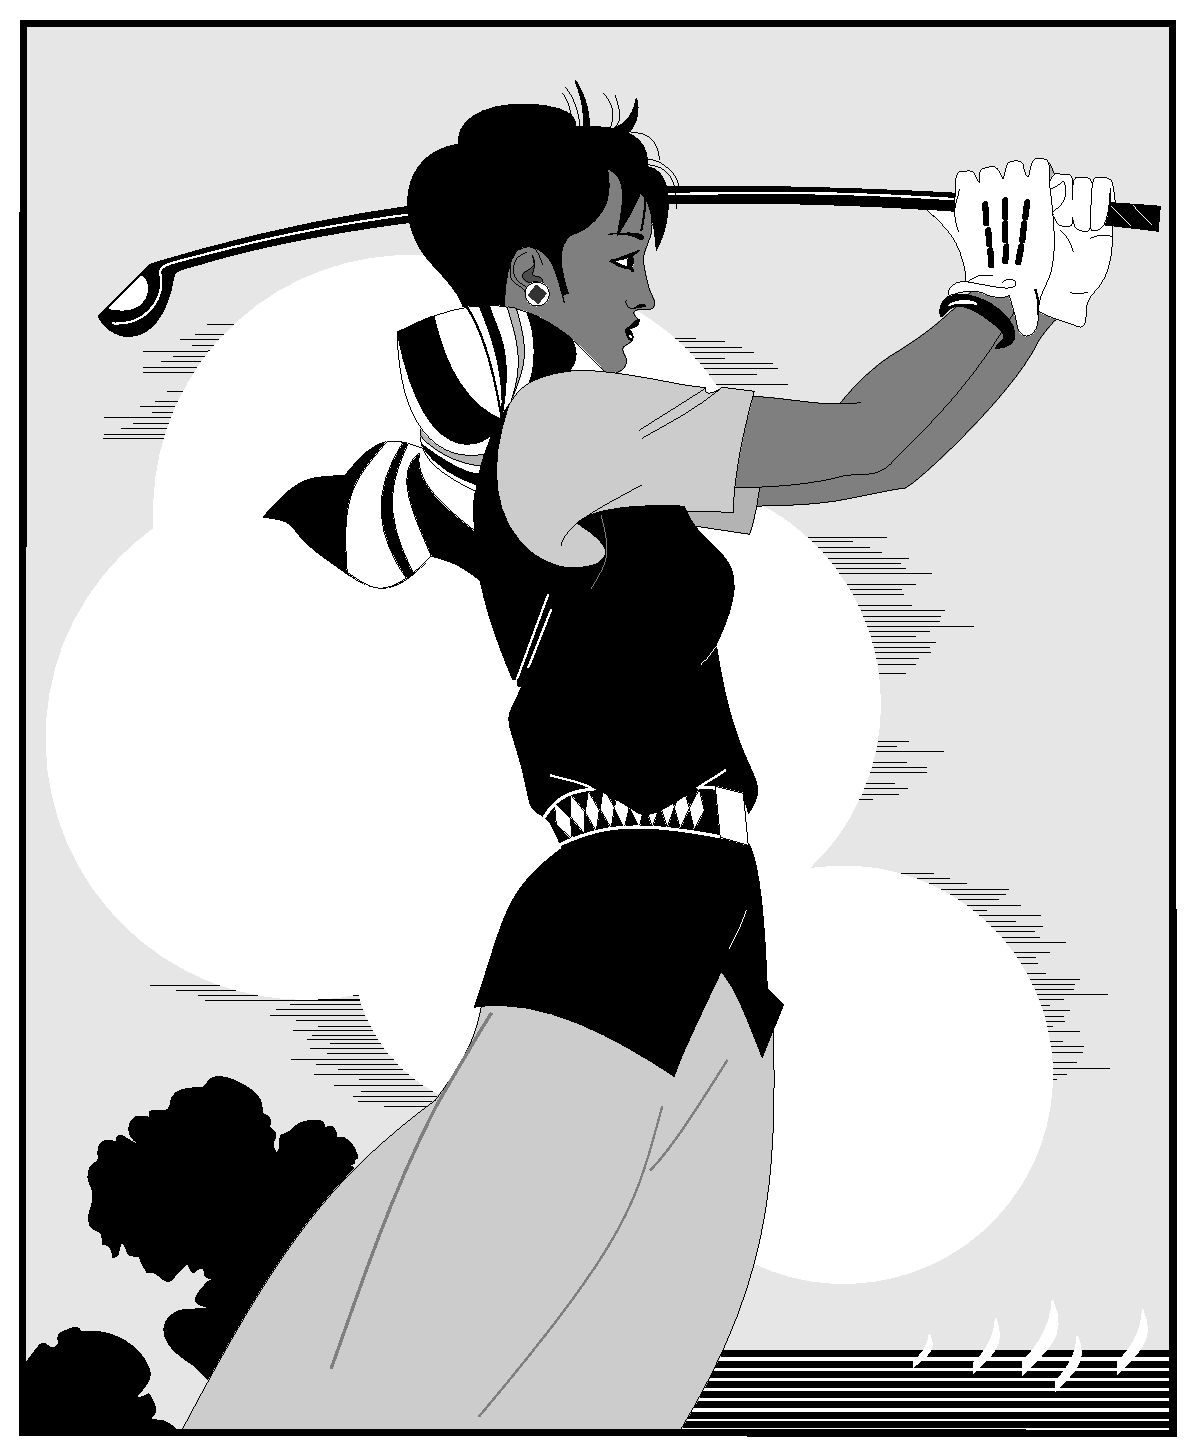
\includegraphics[width=0.2\textwidth]{golfer}}
			\fbox{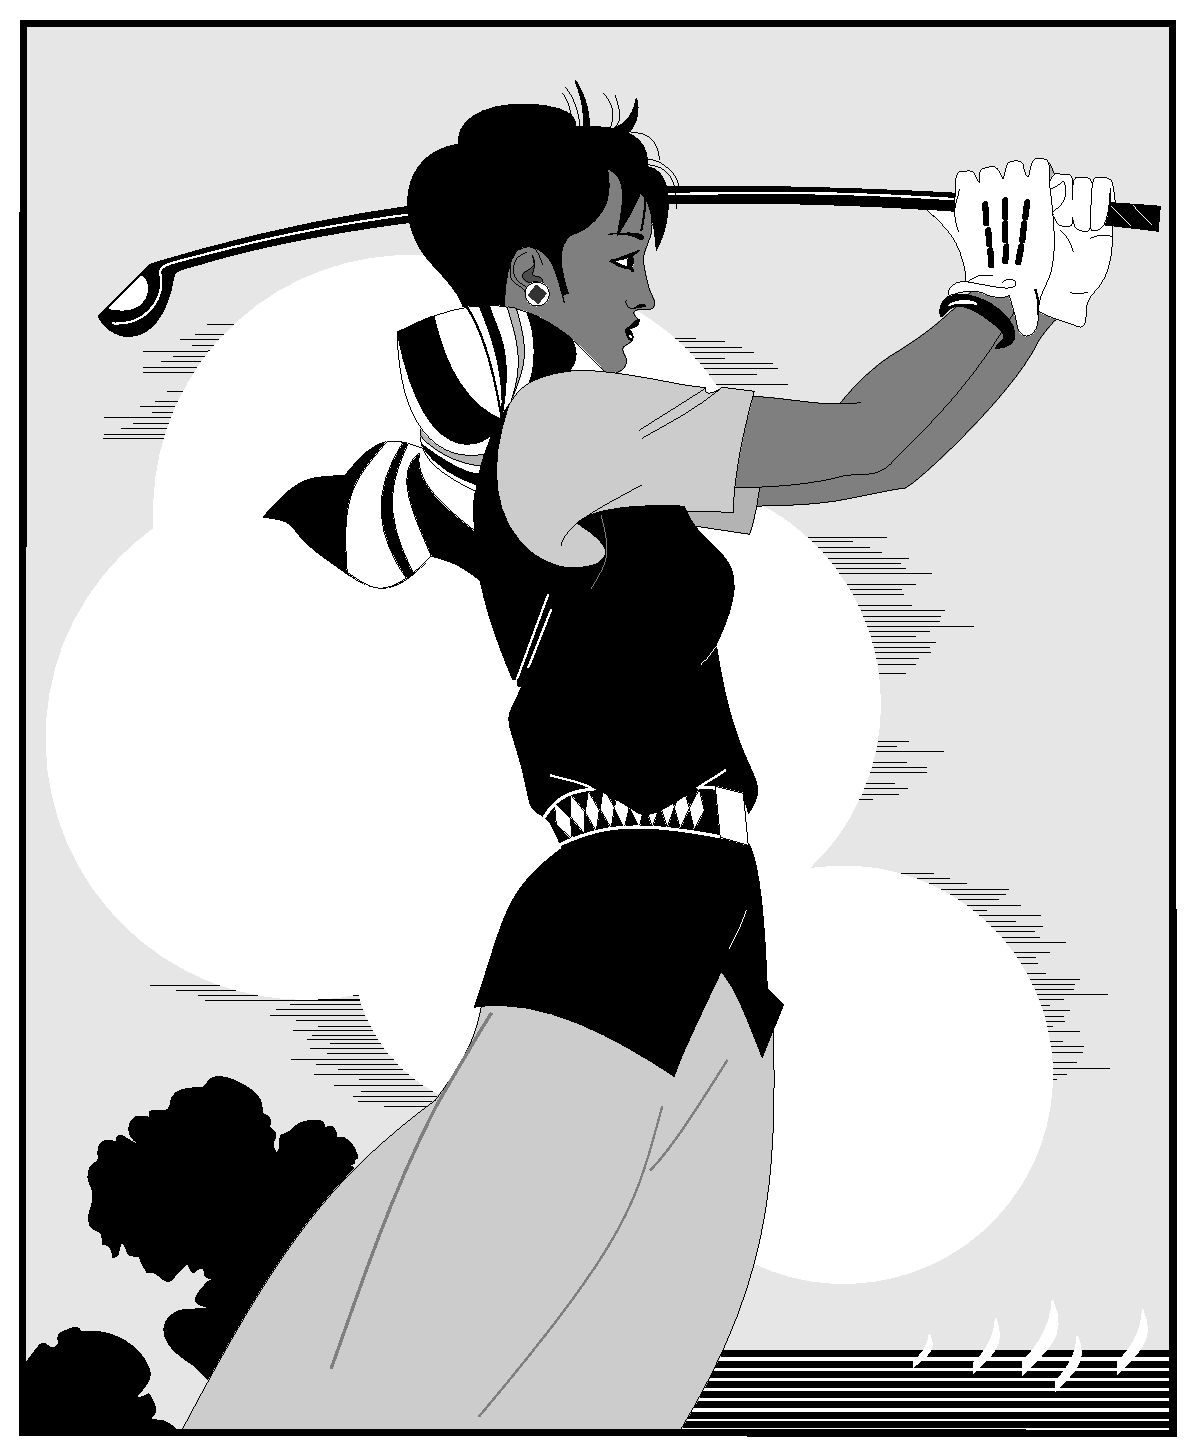
\includegraphics[width=0.2\textwidth]{golfer}}
			\fbox{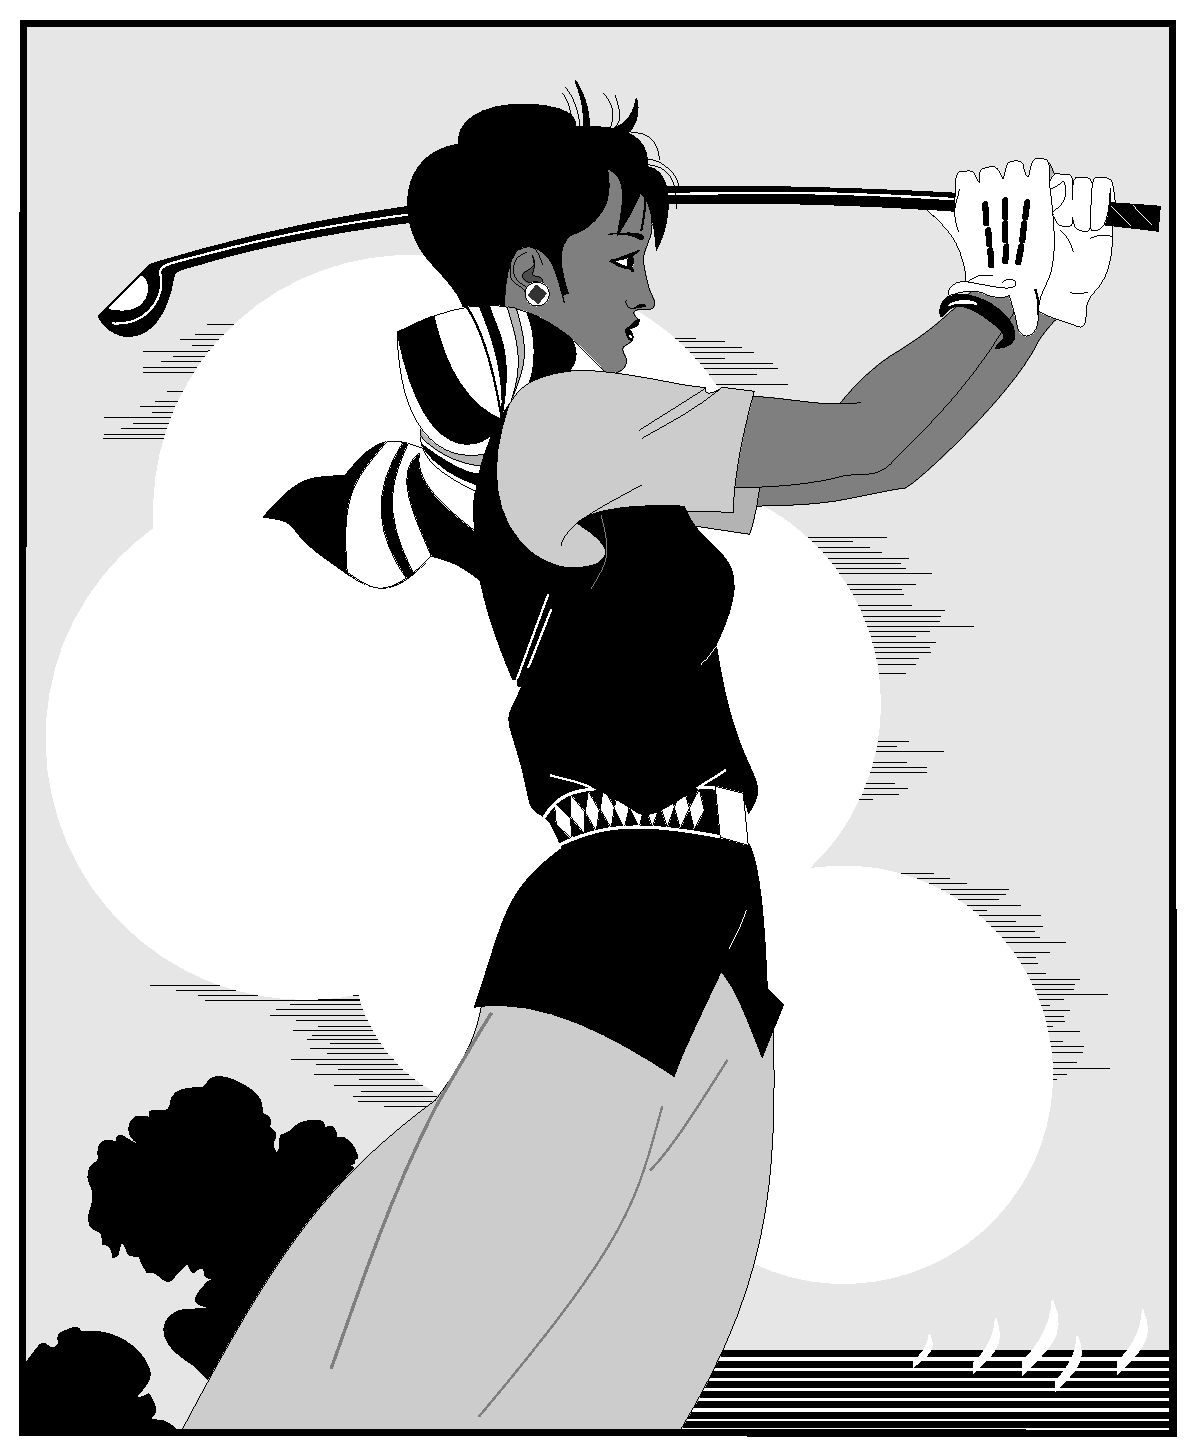
\includegraphics[width=0.2\textwidth]{golfer}}
			\fbox{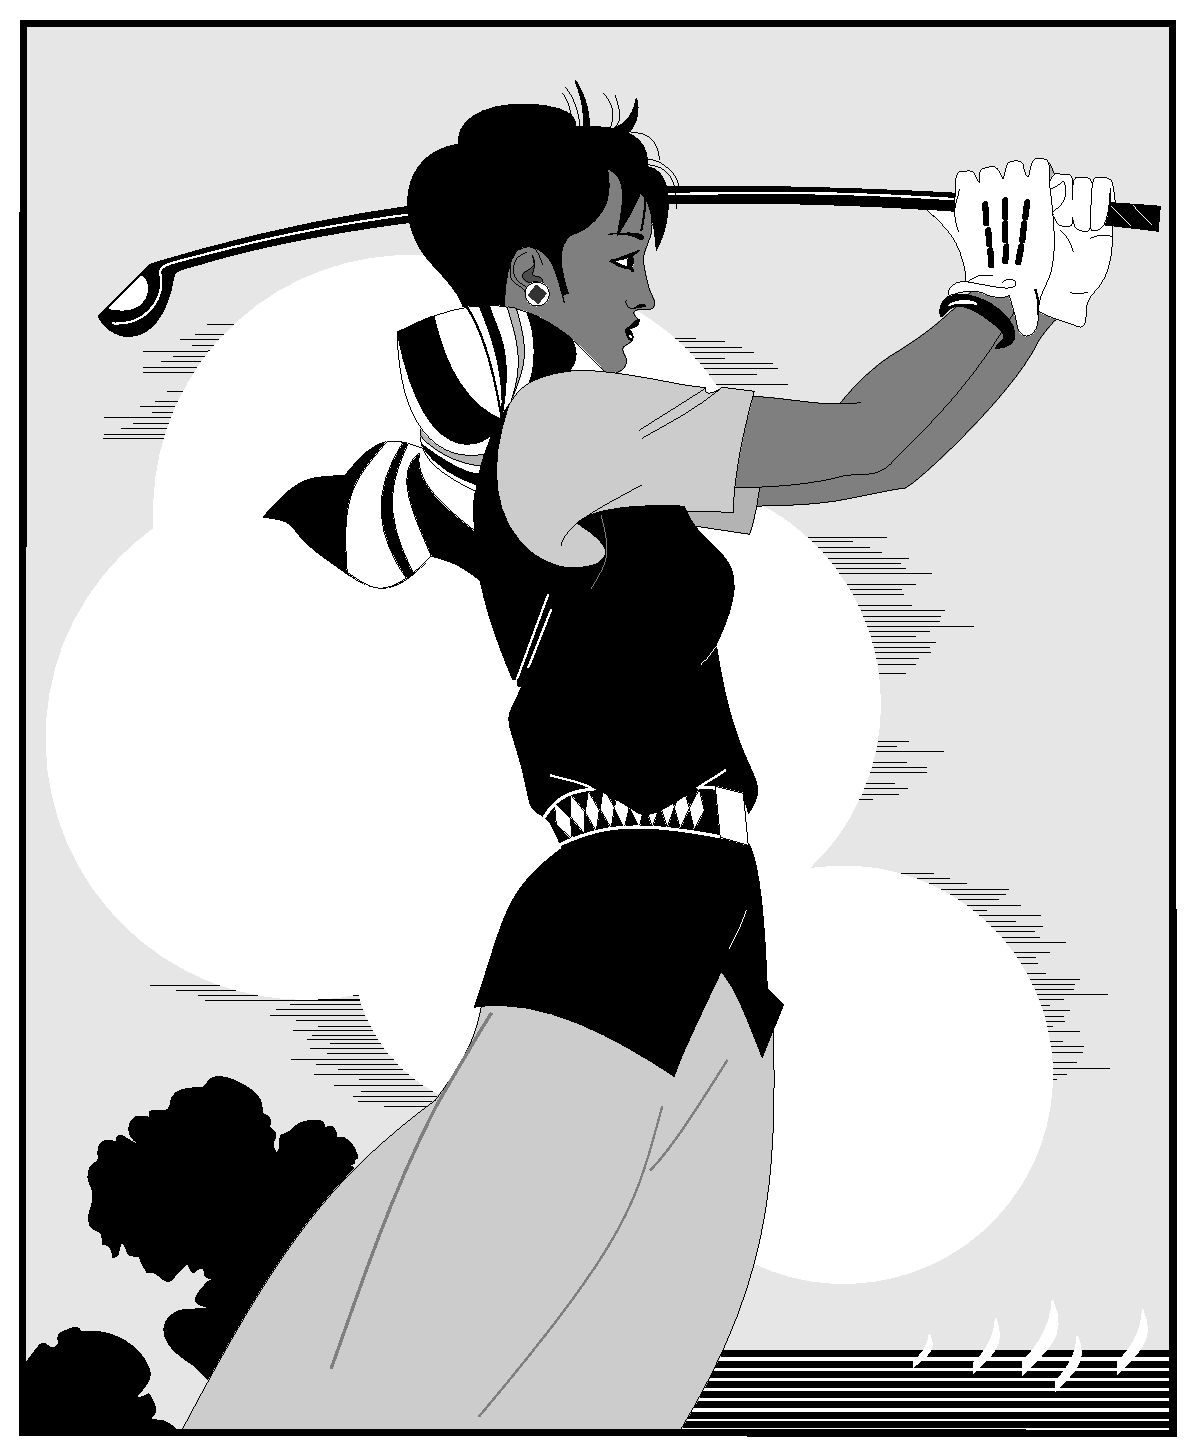
\includegraphics[width=0.2\textwidth]{golfer}}
			\fbox{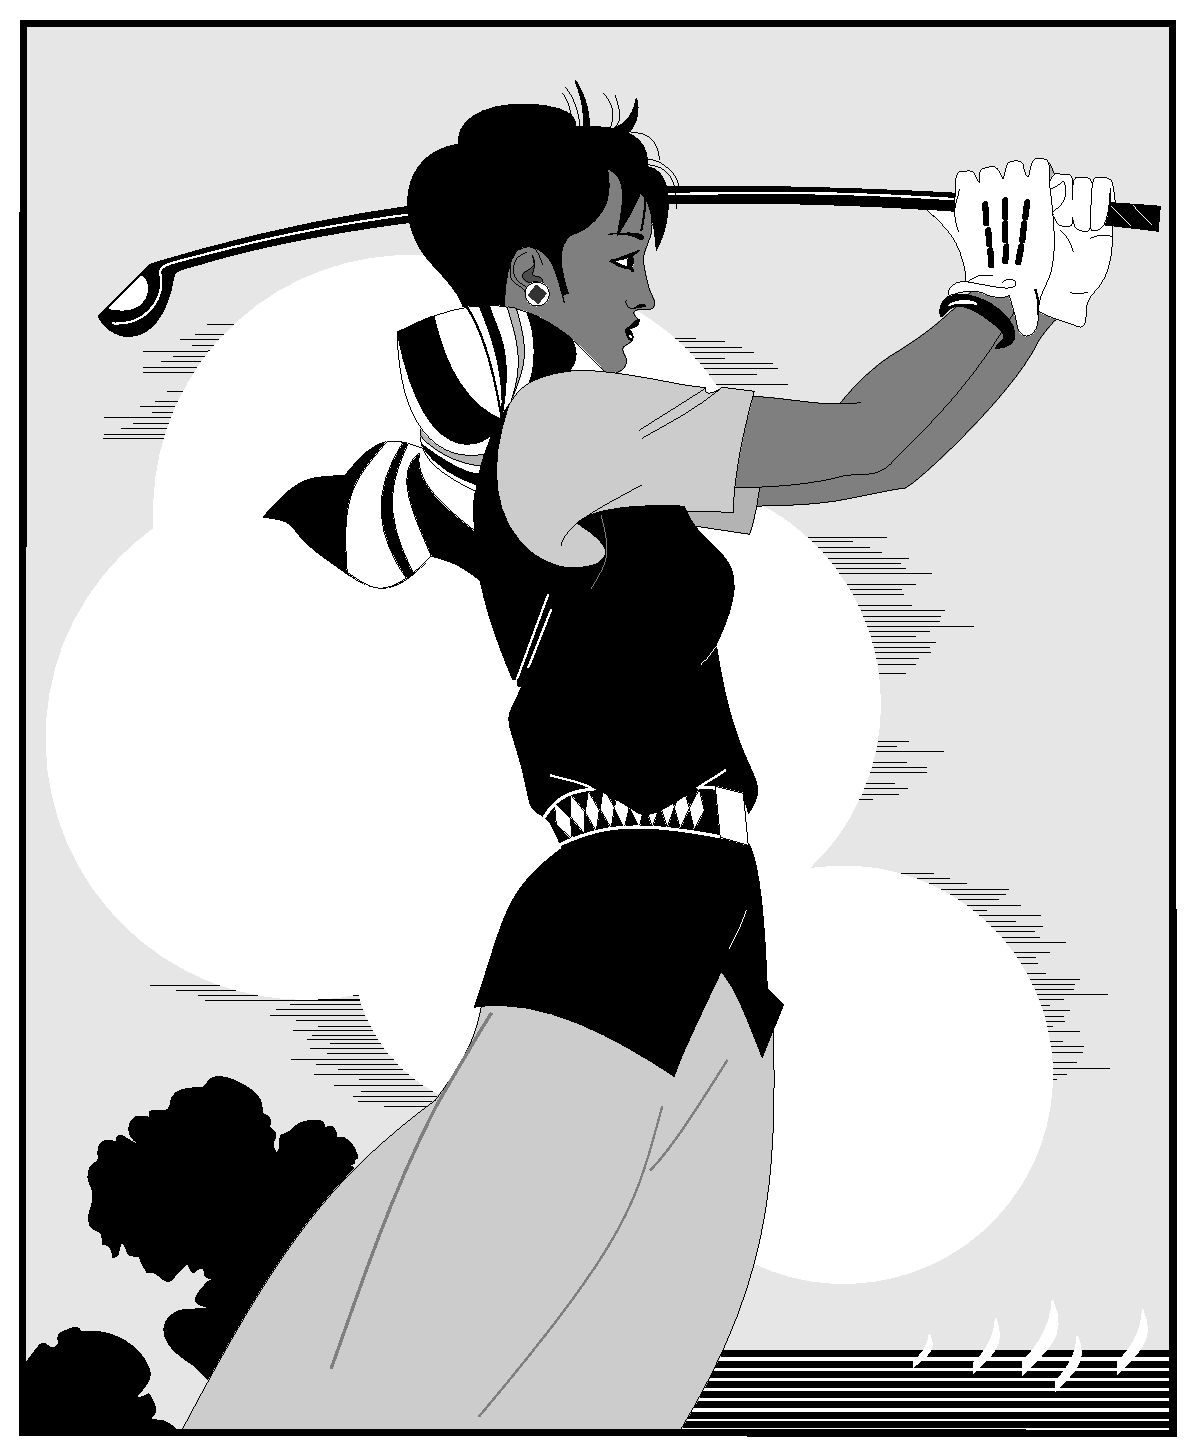
\includegraphics[width=0.2\textwidth]{golfer}}
			\fbox{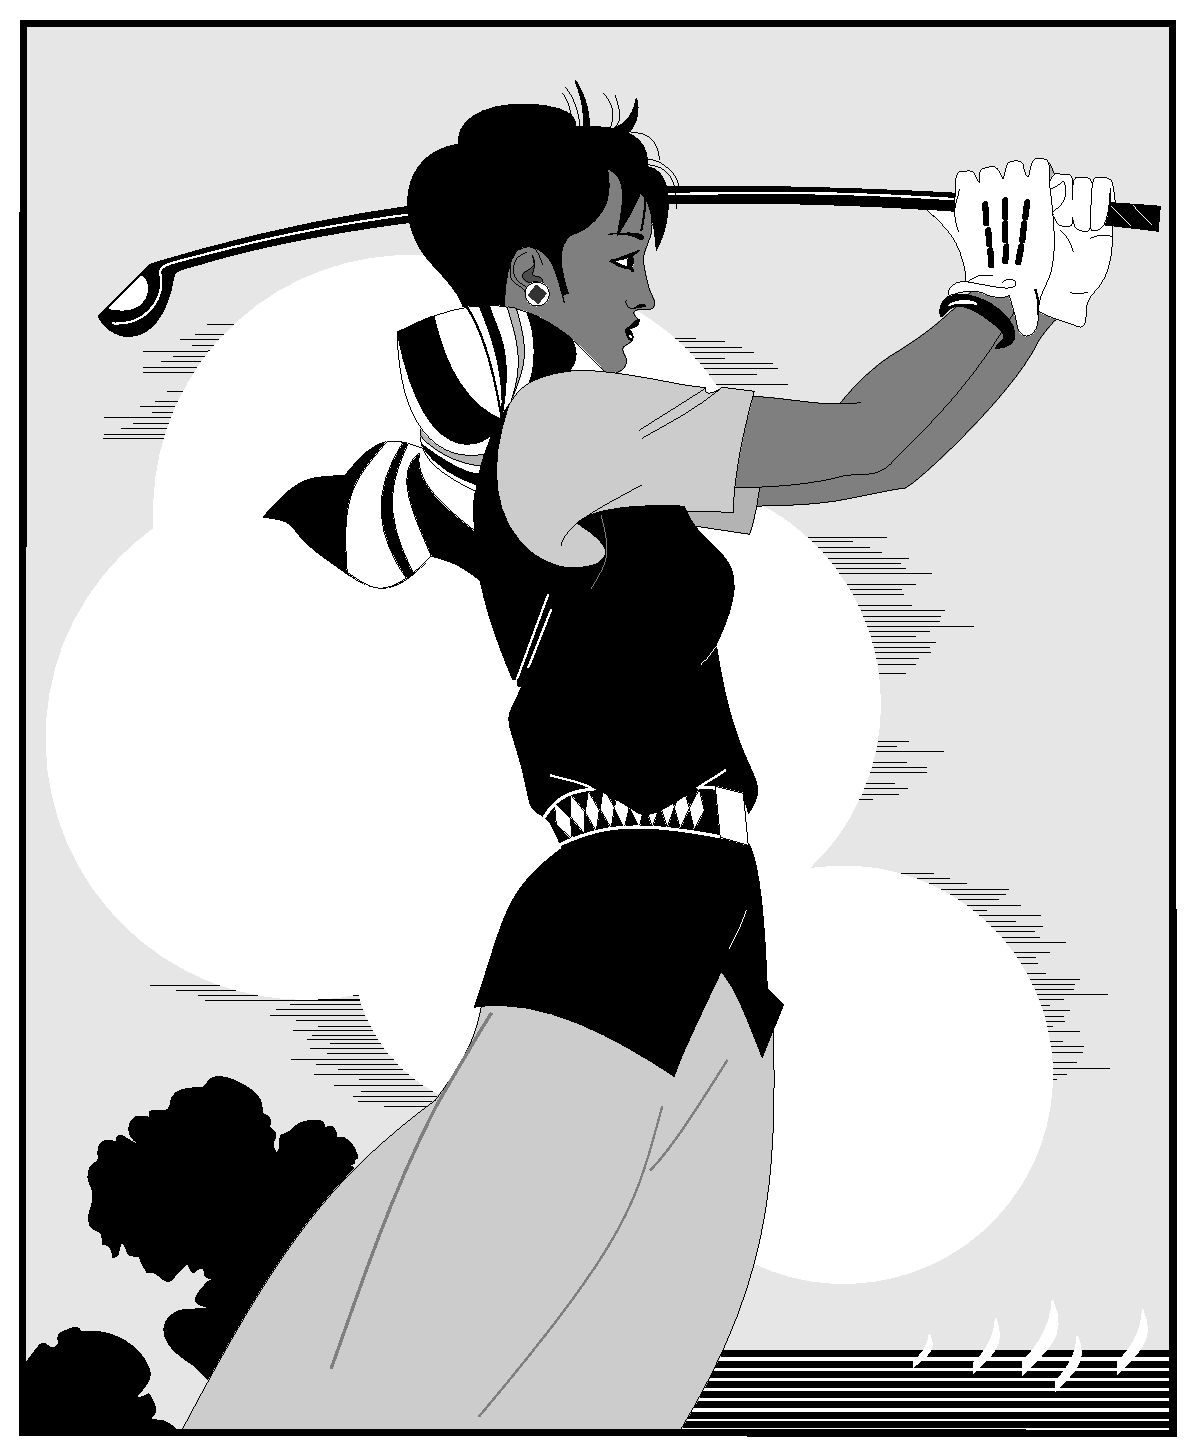
\includegraphics[width=0.2\textwidth]{golfer}}
			\bicaption[golfer7]{}{打高尔夫球的人(非规范要求)}{Fig.$\!$}{The person playing golf (Not stated in the regulation)}
		\end{minipage}
	\end{sideways}
\end{figure}

\clearpage

如果不想让图片浮动到下一章节,那么在此处使用\cs{clearpage}命令。

\section{如何做出符合规范的漂亮的图}
关于作图工具在后文\ref{drawtool}中给出一些作图工具的介绍,此处不多言。
此处以R语言和Tikz为例说明如何做出符合规范的图。

\subsection{Tikz作图举例}
使用Tikz作图核心思想是把格式、主题、样式与内容分离,定义在全局中。
注意字体设置可以有两种选择,如何字少,用五号字,字多用小五。
使用Tikz作图不会出现字体问题,字体会自动与正文一致。

\begin{figure}[thb!]
	\centering
	\begin{tikzpicture}[xscale=0.8,yscale=0.3,rotate=90]
		\small
		\draw (-22,6.5) node[refcell]{参考基因组};
		\draw[refline] (-23, 5) -- (27, 5);
		\draw (-22,3.75) node[tscell]{肿瘤样本};
		\draw (-20,3.75) node[tncell]{正常细胞};
		\draw[tnline] (-21, 2.5) -- (27, 2.5);
		\draw (-20,1.25) node[ttcell]{肿瘤细胞};
		\rcell{2}{6};
		\draw[fakeevolve] (4.5, 5.25) -- (4.5, 4.8);
		\ncell{2}{4};
		\draw[evolve] (4.5, 3) .. controls (4.5,2.8) and (-3.5,2.9) ..  (-3.5, 2);
		\draw[evolve] (4.5, 3) .. controls (4.5,2.8) and (11.5,2.9) .. (11.5, 2);
		\tcellone{-6}{1.5};
		\draw (-9, 2) node[ttcell]{1};
		\draw[evolve] (-3.5, 0) .. controls (-3.5,-0.2) and (-12,-0.1) .. (-12, -1.5);
		\draw[evolve] (-3.5, 0) .. controls (-3.5,-0.2) and (1.5,-0.1) .. (1.5, -1.5);
		\tcellthree{7}{1.5};
		\draw (4, 2) node[ttcell]{2};
		\draw[evolve] (11, 0.5) .. controls (11,0.3) and (19,0.4) .. (19, -1.5);
		\tcellfive{-16}{-2};
		\draw (-19, -1.5) node[ttcell]{3};
		\tcelltwo{-1}{-2};
		\draw (-4, -1.5) node[ttcell]{4};
		\tcellfour{12}{-2};
		\draw (9, -1.5) node[ttcell]{5};
	\end{tikzpicture}
	\begin{minipage}{.9\linewidth}
		\vskip 0.2em
		\wuhao 图中,带有箭头的淡蓝色箭头表示肿瘤子种群的进化方向。一般地,从肿瘤组织中取用于进行二代测序的样本中含有一定程度的正常细胞污染,因此肿瘤的样本中含有正常细胞和肿瘤细胞。每一个子种群的基因组的模拟过程是把生殖细胞变异和体细胞变异加入到参考基因组中。
		\vspace{0.6em}
	\end{minipage}
	\bicaption[tumor]{}{肿瘤组织中各个子种群的进化示意图}{Fig.$\!$}{The diagram of tumor subpopulation evolution process}
\end{figure}

\subsection{R作图}
R是一种极具有代表性的典型的作图工具,应用广泛。
与Tikz图~\ref{tumor}~不同,R作图分两种情况:(1)可以转换为Tikz码;(2)不可转换为Tikz码。
第一种情况图形简单,图形中不含有很多数据点,使用R语言中的Tikz包即可。
第二种情况是图形复杂,含有海量数据点,这时候不要转成Tikz矢量图,这会使得论文体积巨大。
推荐使用pdf或png非矢量图形。
使用非矢量图形时要注意选择好字号(五号或小五),和字体(宋体、新罗马)然后选择生成图形大小,注意此时在正文中使用\cs{includegraphics}命令导入时,不要像导入矢量图那样控制图形大小,使用图形的原本的
宽度和高度,这样就确保了非矢量图形中的文字与正文一致了。

为了控制\hithesis\ 的大小,此处不给出具体举例,

\section{表格}

表应有自明性。表格不加左、右边线。表的编排建议采用国际通行的三线表。表中文字用宋
体~5~号字。每个表格均应有表题(由表序和表名组成)。表序一般按章编排,如第~1~章第
一个插表的序号为“表~1-1”等。表序与表名之间空一格,表名中不允许使用标点符号,表名
后不加标点。表题置于表上,硕士学位论文只用中文,博士学位论文用中、英文两种文字居
中排写,中文在上,要求中文用宋体~5~号字,英文用新罗马字体~5~号字。表头设计应简单
明了,尽量不用斜线。表头中可采用化学符号或物理量符号。


\subsection{普通表格的绘制方法}[Methods of drawing normal tables]

表格应具有三线表格式,因此需要调用~booktabs~宏包,其标准格式如表~\ref{table1}~所示。
\begin{table}[htbp]
	\bicaption[table1]{}{符合研究生院绘图规范的表格}{Table$\!$}{Table in agreement of the standard from graduate school}
	\vspace{0.5em}\centering\wuhao
	\begin{tabular}{ccccc}
		\toprule
		$D$(in) & $P_u$(lbs) & $u_u$(in) & $\beta$ & $G_f$(psi.in) \\
		\midrule
		5       & 269.8      & 0.000674  & 1.79    & 0.04089       \\
		10      & 421.0      & 0.001035  & 3.59    & 0.04089       \\
		20      & 640.2      & 0.001565  & 7.18    & 0.04089       \\
		\bottomrule
	\end{tabular}
\end{table}
全表如用同一单位,则将单位符号移至表头右上角,加圆括号。表中数据应准确无误,书写
清楚。数字空缺的格内加横线“-”(占~2~个数字宽度)。表内文字或数字上、下或左、右
相同时,采用通栏处理方式,不允许用“〃”、“同上”之类的写法。表内文字说明,起行空一
格、转行顶格、句末不加标点。如某个表需要转页接排,在随后的各页上应重复表的编号。
编号后加“(续表)”,表题可省略。续表应重复表头。

\subsection{长表格的绘制方法}[Methods of drawing long tables]

长表格是当表格在当前页排不下而需要转页接排的情况下所采用的一种表格环境。若长表格
仍按照普通表格的绘制方法来获得,其所使用的\verb|table|浮动环境无法实现表格的换页
接排功能,表格下方过长部分会排在表格第1页的页脚以下。为了能够实现长表格的转页接
排功能,需要调用~longtable~宏包,由于长表格是跨页的文本内容,因此只需要单独的
\verb|longtable|环境,所绘制的长表格的格式如表~\ref{table2}~所示。

注意,长表格双语标题的格式。

\vspace{-1.5bp}
\ltfontsize{\wuhao[1.667]}
\wuhao[1.667]\begin{longtable}{ccc}%
	\longbionenumcaption{}{{\wuhao 中国省级行政单位一览}\label{table2}}{Table$\!$}{}{{\wuhao Overview of the provincial administrative unit of China}}{-0.5em}{3.15bp} \\
	%\caption{\wuhao 中国省级行政单位一览}\label{table2}\\
	\toprule 名称 & 简称  & 省会或首府                                                                                                                                \\ \midrule
	\endfirsthead
	\multicolumn{3}{r}{表~\thetable(续表)}\vspace{0.5em}                                                                                                        \\
	\toprule 名称 & 简称  & 省会或首府                                                                                                                                \\ \midrule
	\endhead
	\midrule[0.5pt]
	\endfoot
	\bottomrule
	\endlastfoot
	北京市         & 京   & 北京                                                                                                                                   \\
	天津市         & 津   & 天津                                                                                                                                   \\
	河北省         & 冀   & 石家庄市                                                                                                                                 \\
	山西省         & 晋   & 太原市                                                                                                                                  \\
	内蒙古自治区      & 蒙   & 呼和浩特市                                                                                                                                \\
	辽宁省         & 辽   & 沈阳市                                                                                                                                  \\
	吉林省         & 吉   & 长春市                                                                                                                                  \\
	黑龙江省        & 黑   & 哈尔滨市                                                                                                                                 \\
	上海市         & 沪/申 & 上海                                                                                                                                   \\
	江苏省         & 苏   & 南京市                                                                                                                                  \\
	浙江省         & 浙   & 杭州市                                                                                                                                  \\
	安徽省         & 皖   & 合肥市                                                                                                                                  \\
	福建省         & 闽   & 福州市                                                                                                                                  \\
	江西省         & 赣   & 南昌市                                                                                                                                  \\
	山东省         & 鲁   & 济南市                                                                                                                                  \\
	河南省         & 豫   & 郑州市                                                                                                                                  \\
	湖北省         & 鄂   & 武汉市                                                                                                                                  \\
	湖南省         & 湘   & 长沙市                                                                                                                                  \\
	广东省         & 粤   & 广州市                                                                                                                                  \\
	广西壮族自治区     & 桂   & 南宁市                                                                                                                                  \\
	海南省         & 琼   & 海口市                                                                                                                                  \\
	重庆市         & 渝   & 重庆                                                                                                                                   \\
	四川省         & 川/蜀 & 成都市                                                                                                                                  \\
	贵州省         & 黔/贵 & 贵阳市                                                                                                                                  \\
	云南省         & 云/滇 & 昆明市                                                                                                                                  \\
	西藏自治区       & 藏   & 拉萨市                                                                                                                                  \\
	陕西省         & 陕/秦 & 西安市                                                                                                                                  \\
	甘肃省         & 甘/陇 & 兰州市                                                                                                                                  \\
	青海省         & 青   & 西宁市                                                                                                                                  \\
	宁夏回族自治区     & 宁   & 银川市                                                                                                                                  \\
	新疆维吾尔自治区    & 新   & 乌鲁木齐市                                                                                                                                \\
	香港特别行政区     & 港   & 香港                                                                                                                                   \\
	澳门特别行政区     & 澳   & 澳门                                                                                                                                   \\
	台湾省         & 台   & 台北市                                                                                                                                  \\
\end{longtable}\normalsize
\vspace{-1em}

此长表格~\ref{table2}~第~2~页的标题“编号(续表)”和表头是通过代码自动添加上去的,无需人工添加,若表格在页面中的竖直位置发生了变化,长表格在第~2~页
及之后各页的标题和表头位置能够始终处于各页的最顶部,也无需人工调整,\LaTeX~系统的这一优点是~word~等软件所无法比拟的。

\subsection{列宽可调表格的绘制方法}[Methods of drawing tables with adjustable-width columns]
论文中能用到列宽可调表格的情况共有两种,一种是当插入的表格某一单元格内容过长以至
于一行放不下的情况,另一种是当对公式中首次出现的物理量符号进行注释的情况,这两种
情况都需要调用~tabularx~宏包。下面将分别对这两种情况下可调表格的绘制方法进行阐述
。
\subsubsection{表格内某单元格内容过长的情况}[The condition when the contents in
	some cells of tables are too long]
首先给出这种情况下的一个例子如表~\ref{table3}~所示。
\begin{table}[htbp]
	\centering
	\bicaption[table3]{}{最小的三个正整数的英文表示法}{Table$\!$}{The English construction of the smallest three positive integral numbers}\vspace{0.5em}\wuhao
	\begin{tabularx}{0.7\textwidth}{llX}
		\toprule
		Value & Name  & Alternate names, and names for sets of the given size                                                                                           \\
		\midrule
		1     & One   & ace, single, singleton, unary, unit, unity                                                                                                      \\
		2     & Two   & binary, brace, couple, couplet, distich, deuce, double, doubleton, duad, duality, duet, duo, dyad, pair, snake eyes, span, twain, twosome, yoke \\
		3     & Three & deuce-ace, leash, set, tercet, ternary, ternion, terzetto, threesome, tierce, trey, triad, trine, trinity, trio, triplet, troika, hat-trick     \\
		\bottomrule
	\end{tabularx}
\end{table}
tabularx环境共有两个必选参数:第1个参数用来确定表格的总宽度,第2个参数用来确定每
列格式,其中标为X的项表示该列的宽度可调,其宽度值由表格总宽度确定。标为X的列一般
选为单元格内容过长而无法置于一行的列,这样使得该列内容能够根据表格总宽度自动分行
。若列格式中存在不止一个X项,则这些标为X的列的列宽相同,因此,一般不将内容较短的
列设为X。标为X的列均为左对齐,因此其余列一般选为l(左对齐),这样可使得表格美观
,但也可以选为c或r。

\subsubsection{对物理量符号进行注释的情况}[The condition when physical symbols
	need to be annotated]

为使得对公式中物理量符号注释的转行与破折号“———”后第一个字对齐,此处最好采用表格
环境。此表格无任何线条,左对齐,且在破折号处对齐,一共有“式中”二字、物理量符号和
注释三列,表格的总宽度可选为文本宽度,因此应该采用\verb|tabularx|环境。由
\verb|tabularx|环境生成的对公式中物理量符号进行注释的公式如式(\ref{eq:1})所示。
\begin{equation}\label{eq:1}
	\ddot{\boldsymbol{\rho}}-\frac{\mu}{R_{t}^{3}}\left(3\mathbf{R_{t}}\frac{\mathbf{R_{t}\rho}}{R_{t}^{2}}-\boldsymbol{\rho}\right)=\mathbf{a}
\end{equation}
\begin{tabularx}{\textwidth}{@{}l@{\quad}r@{———}X@{}}
	式中 & $\boldsymbol{\rho}$        & 追踪飞行器与目标飞行器之间的相对位置矢量;               \\
	   & $\boldsymbol{\ddot{\rho}}$ & 追踪飞行器与目标飞行器之间的相对加速度;                \\
	   & $\mathbf{a}$               & 推力所产生的加速度;                          \\
	   & $\mathbf{R_t}$             & 目标飞行器在惯性坐标系中的位置矢量;                  \\
	   & $\omega_{t}$               & 目标飞行器的轨道角速度;                        \\
	   & $\mathbf{g}$               & 重力加速度,$=\frac{\mu}{R_{t}^{3}}\left(
		3\mathbf{R_{t}}\frac{\mathbf{R_{t}\rho}}{R_{t}^{2}}-\boldsymbol{\rho}\right)=\omega_{t}^{2}\frac{R_{t}}{p}\left(
		3\mathbf{R_{t}}\frac{\mathbf{R_{t}\rho}}{R_{t}^{2}}-\boldsymbol{\rho}\right)$,这里~$p$~是目标飞行器的轨道半通径。
\end{tabularx}\vspace{3.15bp}
由此方法生成的注释内容应紧邻待注释公式并置于其下方,因此不能将代码放入
\verb|table|浮动环境中。但此方法不能实现自动转页接排,可能会在当前页剩余空间不够
时,全部移动到下一页而导致当前页出现很大空白。因此在需要转页处理时,还请您手动将
需要转页的代码放入一个新的\verb|tabularx|环境中,将原来的一个\verb|tabularx|环境
拆分为两个\verb|tabularx|环境。

\subsubsection{排版横版表格的举例}[An example of landscape table]

\begin{table}[p]
	\centering
	\begin{sideways}
		\begin{minipage}{\textheight}
			\bicaption[table4]{}{不在规范中规定的横版表格}{Table$\!$}{A table style which is not stated in the regulation}
			\vspace{0.5em}\centering\wuhao
			\begin{tabular}{ccccc}
				\toprule
				$D$(in) & $P_u$(lbs) & $u_u$(in) & $\beta$ & $G_f$(psi.in) \\
				\midrule
				5       & 269.8      & 0.000674  & 1.79    & 0.04089       \\
				10      & 421.0      & 0.001035  & 3.59    & 0.04089       \\
				20      & 640.2      & 0.001565  & 7.18    & 0.04089       \\
				\bottomrule
			\end{tabular}
		\end{minipage}
	\end{sideways}
\end{table}


\section{公式}
与正常\LaTeX\ 使用方法一致,此处略。关于公式中符号样式的定义在`hithesis.sty'有示
例。

\section{其他杂项}[Miscellaneous]

\subsection{右翻页}[Open right]

对于双面打印的论文,强制使每章的标题页出现右手边为右翻页。
规范中没有明确规定是否是右翻页打印。
模板给出了右翻页选项。
为了应对用户的个人喜好,在希望设置成右翻页的位置之前添加\cs{cleardoublepage}命令即可。

\subsection{算法}[Algorithms]
我工算法有以下几大特点。

(1)算法不在规范中要求。

(2)算法常常被使用(至少计算机学院)。

(3)格式乱,甚至出现了每个实验室的格式要求都不一样。

此处不给出示例,因为没法给,在
\href{https://github.com/dustincys/PlutoThesis}{https://github.com/dustincys/PlutoThesis}
的readme文件中有不同实验室算法要求说明。

\subsection{脚注}[Footnotes]
不在再规范\footnote{规范是指\PGR\ 和\UGR}中要求,模板默认使用清华大学的格式。

\subsection{源码}[Source code]
也不在再规范中要求。如果有需要最好使用minted包,但在编译的时候需要添加“
-shell-escape”选项且安装pygmentize软件,这些不在模板中默认载入,如果需要自行载入
。
\subsection{思源宋体}[Siyuan font]
如果要使用思源字体,需要思源字体的定义文件,此文件请到模板的开发版网址github:
\href{https://github.com/dustincys/hithesis}{https://github.com/dustincys/hithesis}
或者oschia:
\href{https://git.oschina.net/dustincys/hithesis}{https://git.oschina.net/dustincys/hithesis}
处下载。

\subsection{专业绘图工具}[Processional drawing tool]
\label{drawtool}
推荐使用tikz包,使用tikz源码绘图的好处是,图片中的字体与正文中的字体一致。具体如
何使用tikz绘图不属于模板范畴。
tikz适合用来画不需要大量实验数据支撑示意图。但R语言等专业绘图工具具有画出各种、
专业、复杂的数据图。R语言中有tikz包,能自动生成tikz码,这样tikz几乎无所不能。
对于排版有极致追求的小伙伴,可以参考
\href{http://www.texample.net/tikz/resources/}{http://www.texample.net/tikz/resources/}
中所列工具,几乎所有作图软件所作的图形都可转成tikz,然后可以自由的在tikz中修改
图中内容,定义字体等等。实现前文窝工规范中要求的图中字体的一致性的终极目标。


\subsection{术语词汇管理}[Manage glossaries]
推荐使用glossaries包管理术语、缩略语,可以自动生成首次全写,非首次缩写。

\subsection{\TeX\ 源码编辑器}[\TeX editor]
推荐:(1)付费软件Winedt;(2)免费软件kile;(3)vim或emaces或sublime等神级编
译器(需要配置)。

\subsection{\LaTeX\ 排版重要原则}[\LaTeX\ typesetting rules]
格式和内容分离是\LaTeX\ 最大优势,所有多次出现的内容、样式等等都可以定义为简单命
令、环境。这样的好处是方便修改、管理。例如,如果想要把所有的表示向量的符号由粗体
\cs{mathbf}变换到花体\cs{mathcal},只需修改该格式的命令的定义部分,不需要像MS
word那样处处修改。总而言之,使用自定义命令和环境才是正确的使用\LaTeX\ 的方式。

\section{关于捐助}
各位刀客和大侠如用的嗨,要解囊相助,请参照图~\ref{zfb}~中提示操作(二维码被矢量化后之后去
除了头像等冗余无用的部分~)。

\begin{figure}[!h]
	\centering\includegraphics[width=0.4\textwidth]{zfb}
	\vspace{0.2em}
	\bicaption[Donation]{}{捐助,注意此处是子图只用汉语图题的形式,我工规定可以不用
		英语图题}{Fig.$\!$}{Donation, please note that it is OK to use Chinese caption
		only}
\end{figure}


% Local Variables:
% TeX-master: "../main"
% TeX-engine: xetex
% End:

\backmatter
% !Mode:: "TeX:UTF-8" 
\begin{conclusions}



本研究针对无监督医学图像配准中面对不同图像域中空间特征变化时对分布外数据配准性能下降的问题,基于互学习范式的配准优化框架,提出了一种结合金字塔结构和自注意力机制的解决思路,取得以下创新性成果:

\begin{enumerate}
    \item 提出了基于互学习配准框架融合金字塔结构与局部注意力机制的解决思路。通过构建异构教师-学生网络体系,将PAN网络的多尺度特征提取能力与RegCST网络的局部优化优势相结合,建立了双向知识蒸馏的递归训练机制,在LPBA40数据集上实现了72.5\%的Dice系数,较单网络训练提升2.8\%。
    \item 验证了体素级可靠性准则(VRC)的动态监督机制的有效性。通过消融实验对比有无VRC模块的配准性能,对于一轮递归训练,使用VRC模块Dice系数相较于未使用提升0.8个百分点,同时SDlogJ指标波动幅度控制在4.3\%以内。
    \item 开发了面向大规模数据的自适应训练策略。针对RegCST网络的显存限制,提出分块循环训练方法,峰值显存占用降低56.7\%;改进的混合损失函数通过动态权重调整机制,使模型收敛速度提升32.1\%,Dice系数在10个训练周期内达到67.3\%。
    \item 构建了多维度评估验证体系。通过解剖结构可视化对齐、差分图像分析与定量指标(Dice、SDlogJ)的综合评估,证实了所提方法的配准优势。
\end{enumerate}

未来工作将在以下方面展开深入研究:

\begin{enumerate}
    \item 拓展互学习框架至多模态配准场景,探索跨模态特征对齐机制。
    \item 研究基于强化学习的递归终止策略,优化训练效率。
    \item 融合拓扑保持约束与生物力学先验知识,进一步提升形变场的生理合理性。
\end{enumerate}

本研究为智能医学影像分析提供了新的理论方法,具有重要的临床应用价值。

\end{conclusions}
   % 结论
\bibliographystyle{gbt7714-numerical}
% \bibliographystyle{gbt7714-numerical-quanjiao} % 全角标点的国标要求的参考文献样式, 哈尔滨硕博用这个
% \bibliographystyle{hitszthesis} % 深圳校区的同学请使用 hitszthesis 文献样式
% \bibliographystyle{hithesis} %理论上2020最新要求文献样式GB/T 7714—2015,但若院系要求文献英文作者不全大写,可改用hithesis文献样式
%%%%%%%%%%%%%%%%%%%%%%%%%%%%%%%%%%%%%%%%%%%%%%%%%%%%%%%%%%%%%%%%%%%%%%%%%%%%%%%%
%-- 注意:以下本硕博、博后书序不一致 --%
%%%%%%%%%%%%%%%%%%%%%%%%%%%%%%%%%%%%%%%%%%%%%%%%%%%%%%%%%%%%%%%%%%%%%%%%%%%%%%%%
% 本科书序(哈尔滨、深圳校区)
%%%%%%%%%%%%%%%%%%%%%%%%%%%%%%%%%%%%%%%%%%%%%%%%%%%%%%%%%%%%%%%%%%%%%%%%%%%%%%%%
\bibliography{reference} % 参考文献
\authorization %授权
% \authorization[scan.pdf] %添加扫描页的命令,与上互斥
% !Mode:: "TeX:UTF-8"
\begin{acknowledgements}

在我完成本论文之际,心中感慨万千,衷心感谢在这段旅程中给予我支持与帮助的人们。首先,我要特别感谢我的指导老师骆功宁教授。您以渊博的知识和严谨的治学态度,给予我悉心的指导和耐心的教诲。在整个毕设过程中,您不仅为我指明了研究的方向,更以您的严谨与热情感染了我,让我在困惑与迷茫中找到了前进的动力。每一次的讨论与交流,都让我豁然开朗,能够顺利完成论文,离不开您的辛勤付出。

同时,我也要感谢我的同学们。在这段重要的时光里,大家的支持与帮助让我倍感温暖。在无数个深夜的图书馆学习时光中,我们相互鼓励,分享经验,共同克服各种困难。无论是对论文的讨论,还是对生活的倾诉,都是我大学生活中的美好瞬间。你们的陪伴,让我在求学路上不再孤单,成为我最宝贵的财富。

此外,我非常感谢我的家人。你们无条件的支持与理解,是我在追求学术道路上最大的动力。在我遇到困难时,你们给予我温暖的鼓励,始终相信我、支持我,帮助我渡过一个又一个难关。感恩有你们的陪伴,才让我拥有了克服挑战的勇气与信心。

我也要感谢验收时各位老师对我论文格式和内容的指导,您们的专业意见与建议使我的论文更加完善。每一位老师的认真审阅和点评都让我获益匪浅,您的严谨与负责让我明白了学术研究的严肃性,也让我学会了在不断修正中追求卓越。

历历浮生,无非败而后成。回首大学四年,我经历了学习的高峰与低谷,收获了知识与友谊,更锻炼了自己的意志与品格。每一个坚持的时刻都在教会我,持之以恒的努力终会迎来丰硕的成果。感谢我自己在这条道路上的坚持与努力,没有放弃,是我走到今天的重要原因。未来的路依然漫长,我会带着这份感恩与勇气,继续前行。

衷心感谢每一位在我人生旅程中给予我帮助的人,愿我们都能在各自的领域中,不断追求卓越,共同成就美好的未来。


\end{acknowledgements}
 %致谢
\begin{appendix}%附录


\chapter{外文资料原文}
\label{cha:engorg}

\title{Unsupervised 3D registration through optimization-guided cyclical self-training}

\textbf{Abstract:}State-of-the-art deep learning-based registration methods employ three different learning strategies: supervised learning, which requires costly manual annotations, unsupervised learning, which heavily relies on hand-crafted similarity metrics designed by domain experts, or learning from synthetic data, which introduces a domain shift. To overcome the limitations of these strategies, we propose a novel selfsupervised learning paradigm for unsupervised registration, relying on self-training. Our idea is based on two key insights. Feature-based differentiable optimizers 1) perform reasonable registration even from random features and 2) stabilize the training of the preceding feature extraction network on noisy labels. Consequently, we propose cyclical self-training, where pseudo labels are initialized as the displacement fields inferred from random features and cyclically updated based on more and more expressive features from the learning feature extractor, yielding a selfreinforcement effect. We evaluate the method for abdomen and lung registration, consistently surpassing metric-based supervision and outperforming diverse state-of-the-art competitors. Source code is available at https://github.com/multimodallearning/reg-cyclical-self-train.

\section{Introduction}

Medical image registration is a fundamental task in medical imaging with applications ranging from multi-modal data fusion to temporal data analysis. In recent years, deep learning has advanced learning-based registration methods [11], which achieve competitive performances at low runtimes and thus constitute a promising alternative to accurate but slow classical optimization methods. A decisive factor in successfully training deep learning-based methods is the choice of a suitable strategy to supervise the learning process. In the literature, there exist three different learning strategies. The first is supervised learning based on manual annotations such as landmark correspondences [9] or semantic labels [16]. However, manual annotations are costly and may introduce a label bias [2]. Alternatively, a second strategy employs synthetic deformation fields to generate image pairs with precisely known displacement fields [7]. However, this introduces a domain gap between synthetic training and real test pairs, limiting the performance at inference time. Elaborated deformation techniques can reduce the gap but require strong domain knowledge, are tailored to specific problems, and do not generalize across tasks. The third widely used training strategy is unsupervised metric-based learning, maximizing a similarity metric between fixed and warped moving images, e.g. implemented in [2,17]. Popular metrics include normalized cross-correlation [19] and MIND [13]. However, the success of this strategy strongly depends on the specific hand-crafted metric, and the performance of the trained deep learning models is often inferior to a classical optimization-based counterpart. Considering the deficiencies of the above training techniques, in this work, we introduce a novel learning strategy for unsupervised registration based on the concept of self-training. Self-training is a widespread training strategy for semi-supervised learning [24] and domain adaptation [29]. The core idea is to pre-train a network on available labeled data and subsequently apply the model to the unlabeled data to generate so-called pseudo labels. Afterwards, one alternates between re-training the model on the union of labeled and pseudo-labeled data and updating the pseudo labels with the current model. This general concept was successfully adapted to diverse tasks and settings, with methods in medical context primarily focusing on segmentation [8,18]. These methods resort to a special form of self-training, the Mean Teacher paradigm [22], where pseudo labels are continuously provided by a teacher model, representing a temporal ensemble of the learning network. A persistent problem of classical and Mean Teacher-based selftraining is the inherent noise of the pseudo labels, which can severely hamper the learning process. As a remedy, some works aim to filter reliable pseudo labels based on model uncertainty [28]. Only recently, the Mean Teacher was adapted to the registration problem, tackling domain adaptation [3] or complementing metric-based supervision for adaptive regularization weighting [25]. Contrary to these methods, we introduce self-training for registration in a fully unsupervised setting, with pseudo labels as the single source of supervision.

\textbf{Contributions.}

We introduce a novel learning paradigm for unsupervised registration by adapting the concept of self-training to the problem. This involves two principal challenges. First, labeled data for the pre-training stage is unavailable, raising the question of how to generate initial pseudo labels. Second, as a general problem in self-training, the negative impact of noise in the pseudo labels needs to be mitigated. In our pursuit to overcome these challenges, we made two decisive observations (see Fig.2) when exploring a combination of deep learning-based feature extraction with differentiable optimization algorithms for the displacement prediction, such as [9,20]. First, we found that feature-based optimizers predict reasonable displacement fields and improve the initial registration even when applied to the output of random feature networks (orange line in Fig.2). We attribute this feature to the inductive bias of deep neural networks, which extract somewhat useful features even with random weights [4]. These predicted displacements thus constitute meaningful initial pseudo labels, solving the first problem and leaving us with the second problem to overcome the noise in the labels. In this context, we made the second observation that the intrinsic regularizing capacity of the optimizers stabilizes the learning from noisy labels. Specifically, training the feature extractor on our initial pseudo labels yielded registrations surpassing the accuracy of the noisy labels used for training (green, red, purple, brown, and magenta lines in Fig.2). Consequently, we propose a cyclical self-training scheme, alternating between training the feature extractor and updating the pseudo labels. As such, our novel learning paradigm does not require costly manual annotations, prevents the domain shift of synthetic deformations, and is independent of hand-crafted similarity metrics. Moreover, our method significantly differs from previous uncertainty-based pseudo label filtering strategies since it implicitly overcomes the negative impact of noisy labels by combining deep feature learning with regularizing differentiable optimization. We evaluate the method for CT abdomen registration and keypoint-based lung registration, demonstrating substantial improvements over diverse state-of-theart comparison methods.

\section{Methods}

\subsection{Problem setup}

Given a data pair ($F$,$M$) of a fixed and a moving image as input, registration aims at finding a displacement field $\varphi$ that spatially aligns $M$ to $F$ . We address the task in an unsupervised setting, where training data $\mathcal{T}=\{(\boldsymbol{F}_i,\boldsymbol{M}_i)\}_{i=1}^{|\mathcal{T}|}$  consists of $|\mathcal{T}|$ unlabeled data pairs. Given the training data, we aim to learn a function $f$ with parameters $\theta_f$ , (partially) represented by a deep network, which predicts displacement fields as $ \hat{\boldsymbol{\varphi}}=f(\boldsymbol{F},\boldsymbol{M};\boldsymbol{\theta}_f)$.

\subsection{Cyclical self-training}

We propose to solve the above problem with a cyclical self-training strategy visualized in Fig.1. While existing self-training methods assume the availability of some labeled data, annotations are unavailable in our unsupervised setting. To overcome this issue and generate an initial set of pseudo labels for the first stage of self-training, we parameterize the function $f$ as the combination of a deep neural network $g$ for feature extraction with a non-learnable but differentiable feature-based optimization algorithm $h$ for displacement prediction, i.e.

\begin{figure}
  \centering
  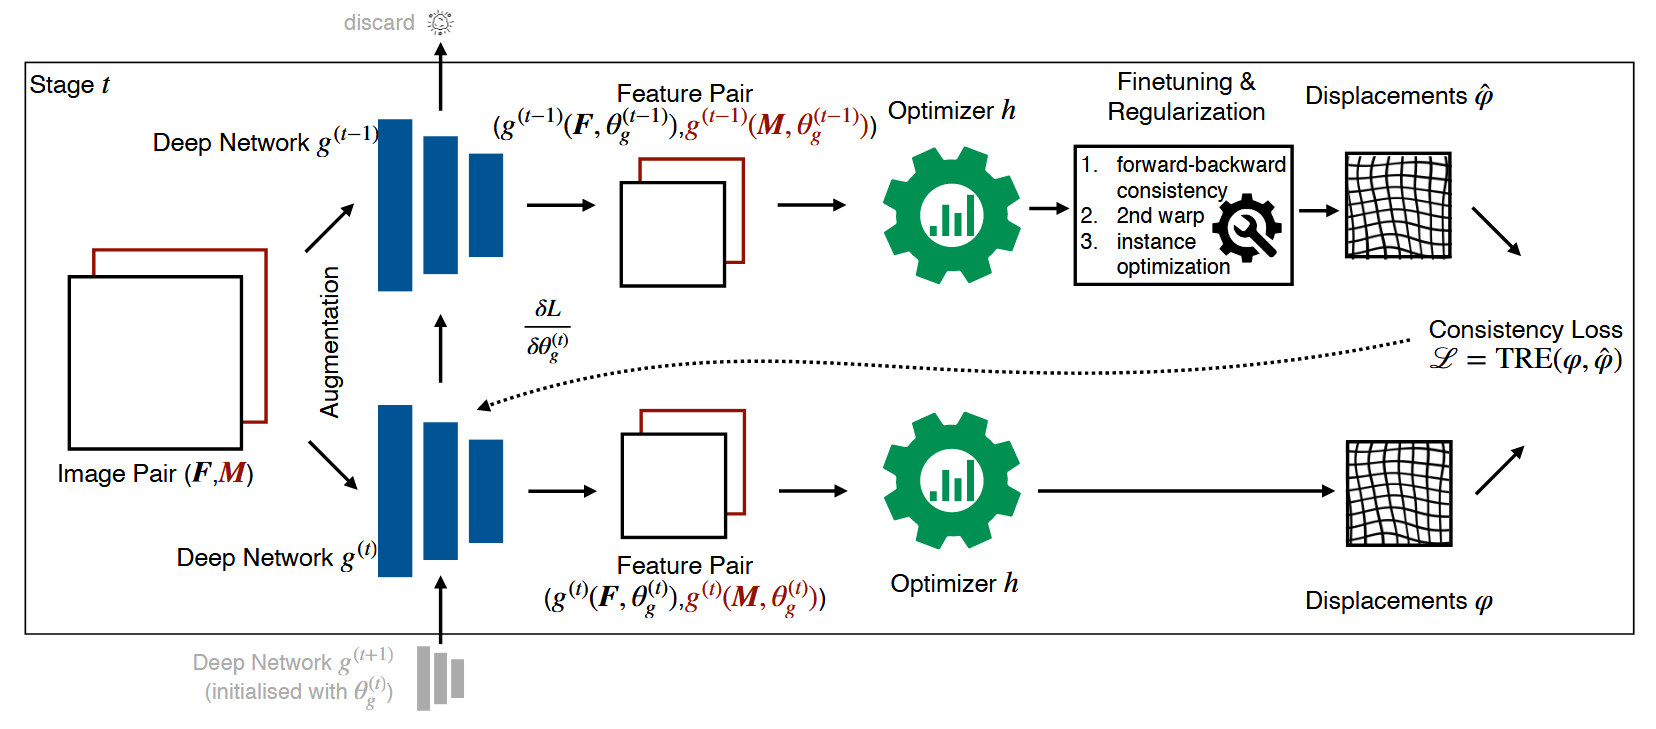
\includegraphics[width=0.9\textwidth]{T_RegCST.png}
  \bicaption[t-fig:1]{无监督注册的循环自训练范式概述}{底层配准流水线包括用于特征提取的深度网络g和用于预测位移的可微优化器h。在阶段t,我们使用基于前一阶段网络g(t-1)的特征生成的伪标签来监督网络g(t)的训练。对于最优特征学习,优化器的伪位移被进一步细化和正则化。}{Fig.$\!$ }{Overview of the proposed cyclical self-training paradigm for unsupervised registration. The underlying registration pipeline comprises a deep network for feature extraction g and a differentiable optimizer h to predict the displacements. At stage t, we supervise the training of the network $g^{(t)}$ with pseudo labels generated based on the features from the network $g^{(t-1)}$ from the previous stage. For optimal feature learning, the pseudo displacements from the optimizer are further refined and regularized.}
\end{figure}

\begin{equation}\tag*{(1)}
  f(\boldsymbol{F},\boldsymbol{M};\boldsymbol{\theta}_f)=h(g(\boldsymbol{F},\boldsymbol{M};\boldsymbol{\theta}_g))
\end{equation}

The approach is based on our empirical observation that a suitable optimization algorithm $h$ can predict reasonable initial displacement fields $\hat{\boldsymbol{\varphi}}^{(0)}$ from random features provided by a network $g^{(0)}$ with random initialization$\theta_G^{(0)} $, which is in line with recent studies on the inductive bias of CNNs [4]. We leverage these predicted displacements as pseudo labels to supervise the first stage of self-training,where the parameters of the feature extractor with different initialization$\theta_G^{(1)} $are optimized by minimizing the loss

\begin{equation}\tag*{(2)}
  \mathcal{L}(\boldsymbol{\theta}_g^{(1)};\mathcal{T})=\frac{1}{|\mathcal{T}|}\sum_i\mathrm{TRE}\left(h\left(g\left(\boldsymbol{F}_i,\boldsymbol{M}_i;\boldsymbol{\theta}_g^{(1)}\right)\right),\hat{\boldsymbol{\varphi}}_i^{(0)}\right)
\end{equation}

with $\mathrm{TRE}(\hat{\boldsymbol{\varphi}}_\mathrm{i}^{(1)},\hat{\boldsymbol{\varphi}}_\mathrm{i}^{(0)})$ denoting the mean over the element-wise target registration error between the displacement fields $\hat{\boldsymbol{\varphi}}_\mathrm{i}^{(1)} $ and $\hat{\boldsymbol{\varphi}}_\mathrm{i}^{(0)}$.

A critical problem of this basic setup is that the network might overfit the initial pseudo labels and learn to reproduce random features. Therefore, in the spirit of recent techniques from contrastive learning [6], we propose to improve the efficacy of feature learning by incorporating asymmetries into the learning and pseudo label streams at two levels. First, we apply different random augmentations to the input pairs in both streams. Second, we augment the pseudo label stream with additional (non-differentiable) fine-tuning and regularization steps after the optimizer to improve the pseudo displacement fields (see Sec. 2.3 for details). As demonstrated in our ablation experiments (Fig.2, Tab.1), both strategies improve feature learning and strengthen the self-improvement effect.

Once the first stage of self-training has converged, we repeat the process $T$ times. Specifically, at stage $t$, we generate refined pseudo labels with the trained network $g^{(t-1)}$ from the previous stage, initialize the learning network $g^{(t)}$ with the weights from $g^{(t-1)}$ and perform a warm restart on the learning rate to escape potential local minima from the previous stage.

\subsection{Registration framework}

Our proposed self-training scheme is a flexible, modular framework, agnostic to the input modality and the specific implementation of feature extractor $g$ and optimizer $h$. This section describes our specific design choices for $g$ and $h$ for image and point cloud registration, with the former being our main focus.


\textbf{Image registration.} To extract features from 3D input volumes, we implement g a standard 3D CNN with six convolution layers with kernel sizes 3 $\times$ 3 $\times$ 3 and 32, 64, or 128 channels. Each convolution is followed by BatchNorm and ReLU, and every second convolution contains a stride of 2, yielding a downsampling factor of 8. The outputs for both images are mapped to 16-dimensional features using a 1 $\times$ 1 $\times$ 1 convolution and fed into a correlation layer [21] that captures 125 discrete displacements.

As the optimizer, we adapt the coupled convex optimization for learningbased 3D registration from [20], which, given fixed and moving features, infers a displacement field that minimizes a combined objective of smoothness and feature dissimilarity. Our proposed refinement strategy in the pseudo label stream comprises three ingredients. 1) Forward-backward consistency additionally computes the reverse displacement field ($\boldsymbol{F}$ to $\boldsymbol{M}$ ) and then iteratively minimizes the discrepancy between both fields. 2) For a second warp, the moving image is warped with the inferred displacement field before repeating all previous steps. 3) Iterative instance optimization finetunes the final displacement field with Adam by jointly minimizing regularization cost and feature dissimilarity. For the latter, we use the CNN features after the second convolution block and map them with a 1$\times$1$\times$1 convolution to 16 channels. We apply the same refinement steps at test time. Moreover, we propose to leverage the difference between network-predicted and finetuned displacements to estimate the difficulty of the training samples. Consequently, we apply a weighted batch sampling at training that increases the probability of using less difficult registration pairs with a higher agreement between both fields. We rank all training pairs and use a sigmoid function with arguments ranging linearly from -5 to 5 for the weighted random sampler.

\textbf{Point cloud registration.} For point cloud registration, we implement the feature extractor as a graph CNN and rely on sparse loopy belief propagation for differentiable optimization, as introduced in [9].

\section{Experiments}

\subsection{Experimental setup}

\textbf{Datasets.} We conduct our main experiments for inter-patient abdomen CT registration using the corresponding dataset of the Learn2Reg (L2R) Challenge [15]. The dataset contains 30 abdominal 3D CT scans of different patients with 13 manually labeled anatomical structures of strongly varying sizes. The original image data and labels are from [26]. As part of L2R, they were affinely preregistered into a canonical space and resampled to identical voxel resolutions (2 mm) and spatial dimensions (192 $\times$ 160 $\times$ 256 vx). Following the data split of L2R, we use 20 scans (190 pairs) for training and the remaining 10 scans (45 pairs) for evaluation. Hence, data split and preprocessing are consistent with compared previous works [9,27]. As metrics, we report the mean Dice overlap (DSC) between the semantic labels and the standard deviation of the logarithmic Jacobian determinant (SDlogJ).

We perform a second experiment for inhale-to-exhale lung CT registration on the DIR-Lab COPDGene dataset5 [5], which comprises 10 such scan pairs. For each pair, 300 expert-annotated landmark correspondences are available for evaluation. We pre-process all scans in multiple steps: 1) resampling to 1.75$\times$1.00$\times$1.25 mm for exhale and 1.75$\times$1.25$\times$1.75 mm for inhale, 2) cropping with fixed-size bounding boxes (192 $\times$ 192 $\times$ 208 vx), centered around automatically generated lung masks, 3) affine pre-registration, aligning the lung masks. Since we focus on keypoint-based registration of the lung CTs, we follow [9] and extract distinctive keypoints from the CTs using the Förstner algorithm with non-maximum suppression, yielding around 1k points in the fixed and 2k points in the moving cloud. In our experiments, we perform 5-fold cross-validation, with each fold comprising eight data pairs for training and two for testing. We report the target registration error (TRE) at the landmarks and the SDlogJ as metrics.

\textbf{Implementation details.} We implement all methods in Pytorch and optimize network parameters with the Adam optimizer. For abdomen registration, we train for $T$ = 8 stages, each stage comprising 1000 iterations with a batch size of 2. The learning rate follows a cosine annealing warm restart schedule, decaying from $10^{-3}$ to $10^{-5}$ at each stage. Hyper-parameters were set based on the DSC on three cases from the training set. For lung registration, the model converged after $T$ = 5 stages of 60 epochs with batch size 4, with an initial learning rate of 0.001, decreased by a factor of 10 at epochs 40 and 52. Here, hyper-parameters were adopted from [9]. For both datasets, training requires 90-100 min and 8 GB on an RTX2080, and input augmentations consist of random affine transformations.

\subsection{Results}

\textbf{Abdomen. }First, we analyze our method in several ablation experiments. In Fig.2, we visualize the performance of our method on a subset of classes over several cycles of self-training. We observe consistent improvements over the stages, particularly pronounced at early stages while the performance converges later on. This highlights the self-reinforcing effect achieved through alternating pseudo label updates and network training. In the upper part of Tab.1, we verify the efficacy of incorporating asymmetries (input augmentations, finetuning of pseudo labels) into both streams and weighted sampling. The results confirm the importance of each component to reach optimal performance. In the lower part of Tab.1, we evaluate our final model under different test configurations, highlighting the improvements through a second warp and Adam finetuning.

\begin{figure}
  \centering
  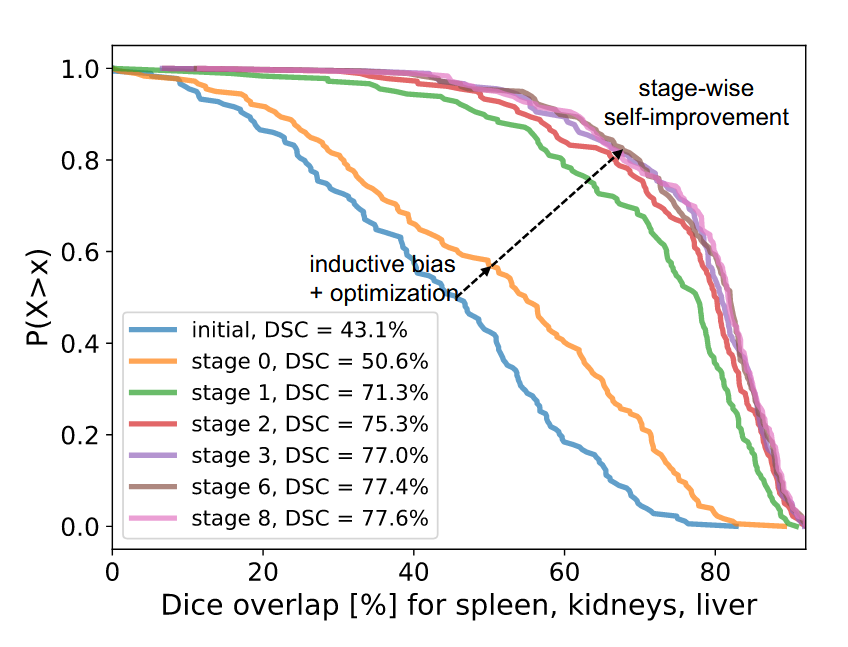
\includegraphics[width=0.9\textwidth]{T_result.png}
  \bicaption[t-fig:2]{}{在不同阶段的自我训练后,腹部CT登记的Dice重叠的“相反”累积分布。}{Fig.$\!$ }{“Opposite” cumulative distribution of Dice overlaps for Abdomen CT registration after different stages of self-training.}
\end{figure}

\begin{table}
  \bicaption[t:table1]{}{腹部CT配准的消融研究。}{Table$\!$}{Ablation study for abdomen CT registration.}
  \vspace{0.5em}\centering\wuhao
  \begin{tabular}{lcc}
    \toprule
    \textbf{Method}       & \textbf{DSC}  & \textbf{SDlogJ} \\
    \midrule
    prealign              & 25.9          & --              \\
    w/o input augm.       & 48.8          & 0.129           \\
    w/o PL refinement     & 48.8          & 0.200           \\
    w/o weighted sampling & 50.1          & 0.147           \\
    ours                  & 51.1          & 0.146           \\
    \midrule
    1 warp w/o Adam       & 38.6          & 0.061           \\
    1 warp w/ Adam        & 49.6          & 0.119           \\
    2 warps w/o Adam      & 41.1          & 0.088           \\
    2 warps w/Adam (ours) & \textbf{51.1} & 0.146           \\
    \bottomrule
  \end{tabular}
\end{table}

Next, we compare our method to a comprehensive set of state-of-the-art unsupervised methods, including classical algorithms [1,10,14] and deep learningbased approaches, trained with MIND [2,12]/NCC [17] supervision or contrastive learning [27]. The results are collected from [9] and [27]. Moreover, we train our own registration framework with metric-based supervision (MIND [13], NCC [19]) to directly verify the advantage of our self-training strategy. Results are shown in Tab.2, Fig.3, and Supp., Fig.3. Our method substantially outperforms all comparison methods in terms of DSC (statistical significance is confirmed by a Wilcoxon-signed rank test with p<0.0001 for all competitors with public code, which excludes SAME) and sets a new state-of-the-art accuracy of 51.1\% DSC. This highlights the advantages of our new learning paradigm over previous unsupervised strategies. Meanwhile, the smoothness of predicted displacement fields (SDlogJ) is comparable with most unsupervised deep learning-based methods [2,12] and superior to MIND- and NCC-supervision.

\begin{figure}
  \centering
  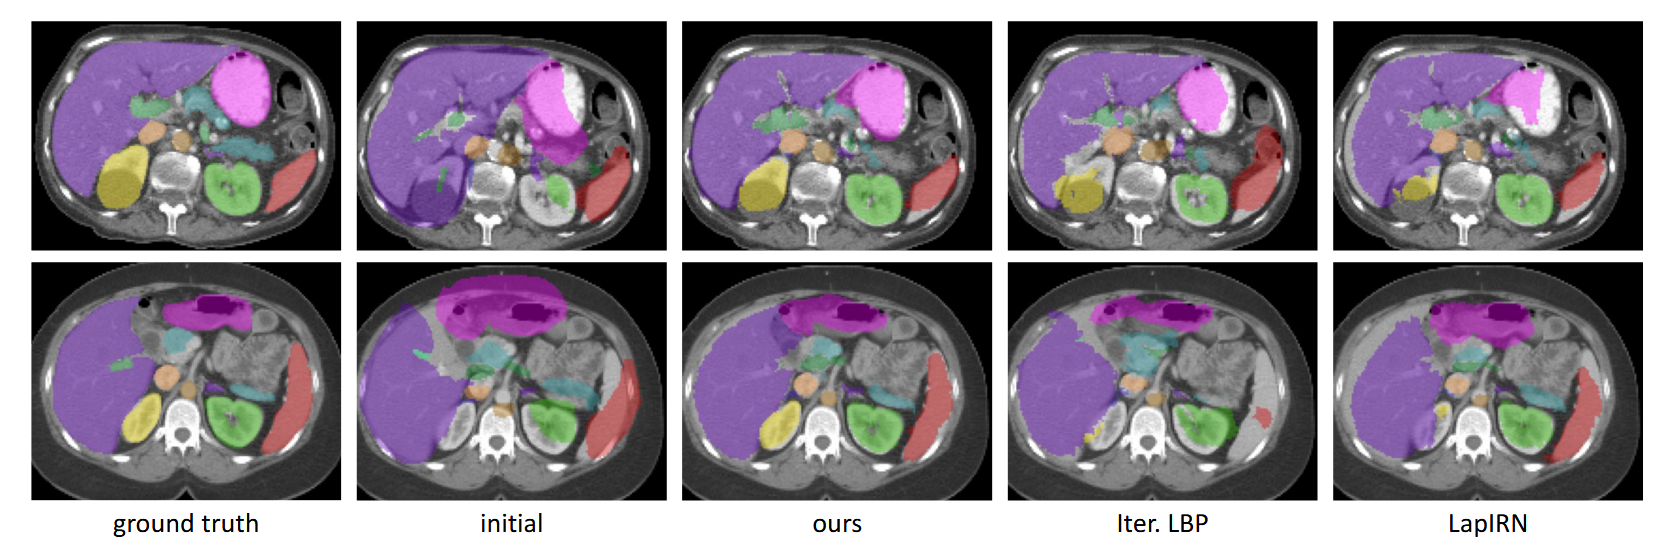
\includegraphics[width=0.9\textwidth]{T_img.png}
  \bicaption[t-fig:3]{}{所选方法对两例腹部CT数据集(轴向视图)的定性结果。我们展示了扭曲分割标签与固定扫描的叠加}{Fig.$\!$ }{Qualitative results of selected methods on two cases of the Abdomen CT dataset (axial view). We show overlays of the warped segmentation labels with the fixed scan.}
\end{figure}

\begin{table}
  \bicaption[t:table2]{}{无监督腹部CT配准结果}{Table$\!$}{Results for unsupervised abdomen CT registration.}
  \vspace{0.5em}\centering\wuhao
  \begin{tabular}{lccc}
    \toprule
    \textbf{Method} & \textbf{Dice [\%]} & \textbf{SDlogJ} & \textbf{Time [s]} \\
    \midrule
    pre-aligned     & 25.9               & --              & --                \\
    Adam            & 36.6               & 0.080           & 1.6               \\
    Iter. LBP       & 40.1               & 0.093           & 0.6               \\
    ANTs (SyN)      & 28.4               & {N/A}           & 74.3              \\
    DEEDS           & 46.5               & {N/A}           & 45.4              \\
    \midrule
    VoxelMorph      & 35.4               & 0.134           & 0.2               \\
    PDD             & 41.5               & 0.129           & 1.4               \\
    LapIRN          & 42.4               & 0.089           & 3.8               \\
    SAME            & 49.8               & {N/A}           & 1.2               \\
    \midrule
    MIND sup.       & 47.7               & 0.237           & 1.2               \\
    NCC sup.        & 48.1               & 0.299           & 1.2               \\
    \midrule
    ours            & \textbf{51.1}      & 0.146           & 1.2               \\
    \bottomrule
  \end{tabular}
\end{table}

\textbf{Lung. }For point cloud-based lung registration, we compare our cyclical selftraining strategy to three alternative learning strategies: supervision with manually annotated landmark correspondences as in [9], metric-based supervision with Chamfer distance and local Laplacian penalties as in [23], and training on synthetic rigid/random field deformations. All strategies are implemented for the same baseline registration model from [9]. Moreover, we report the performance of three unsupervised image-based deep learning methods [2,12,17] trained with MIND supervision. Results are shown in Tab.3, demonstrating the superiority of our self-training strategy over all competing learning strategies and the reported image-based SOTA methods. Qualitative results of the experiment are shown in Supp., Fig.4, demonstrating accurate and smooth displacements, as also confirmed by low values of SDlogJ.

\begin{table}
  \bicaption[t:table3]{}{COPD数据集上的肺部CT配准结果}{Table$\!$}{Results for lung CT registration on the COPD dataset.}
  \vspace{0.5em}\centering\wuhao
  \begin{tabular}{lcc}
    \toprule
    \textbf{Method}       & \textbf{TRE [mm]} & \textbf{SDlogJ} \\
    \midrule
    initial (pre-aligned) & 11.99             & --              \\
    VoxelMorph            & 7.98              & {N/A}           \\
    LapIRN                & 4.99              & {N/A}           \\
    PDD                   & 2.16              & {N/A}           \\
    \midrule
    rigid deform.         & 2.98              & 0.037           \\
    rnd. field deform.    & 3.19              & 0.035           \\
    metric sup.           & 6.79              & 0.042           \\
    landmark sup.         & 2.27              & 0.036           \\
    \midrule
    ours                  & \textbf{1.93}     & 0.033           \\
    \bottomrule
  \end{tabular}
\end{table}

\section{Conclusion}

We introduced a novel cyclical self-training paradigm for unsupervised registration. To this end, we developed a modular registration pipeline of a deep feature extraction network coupled with a differentiable optimizer, stabilizing learning from noisy pseudo labels through regularization and iterative, cyclical refinement. That way, our method avoids pitfalls of popular metric supervision (NCC, MIND), which relies on shallow features or image intensities and is prone to noise and local minima. By contrast, our supervision through optimization-refined and -regularized pseudo labels promotes learning task-specific features that are more robust to noise, and our cyclical learning strategy gradually improves the expressiveness of features to avoid local minima. In our experiments, we demonstrated the efficacy and flexibility of our approach, which outperformed the competing state-of-the-art methods and learning strategies for dense image-based abdomen and point cloud-based lung registration. In summary, we did not only present the first fully unsupervised self-training scheme but also a new perspective on unsupervised learning-based registration. In particular, we consider our strategy complementary to existing techniques (metric-based and contrastive learning), opening up the potential for combined training schemes in future work.



\chapter{外文资料翻译}
\label{cha:chorg}
\title{基于优化引导循环自训练的无监督三维配准方法}
\textbf{摘要:}当前最先进的深度学习配准方法采用三种学习策略:需要昂贵人工标注的监督学习、严重依赖领域专家设计的人工相似性度量的无监督学习,以及存在领域偏移问题的合成数据训练方法。为了克服这些策略的局限,我们提出了一种基于自训练机制的新型自监督学习范式。该方法基于两个关键洞见:1)基于特征的可微分优化器即使使用随机特征也能完成合理配准;2)该优化器能稳定特征提取网络在噪声标签下的训练。因此我们提出循环自训练框架:首先通过随机特征推导位移场初始化伪标签,随后基于特征提取网络生成的增强特征循环更新伪标签,最终形成自我强化效应。在腹部和肺部配准任务上的实验表明,本方法显著超越基于相似性度量的监督方法,性能优于多种当前最先进的对比方法。源码详见 https://github.com/multimodallearning/reg-cyclical-self-train。

\section{介绍}

医学图像配准是医学影像领域的基础任务,其应用涵盖多模态数据融合及时序数据分析等多个方面。近年来,深度学习推动了基于学习的配准方法发展[11],这些方法在保证较低运行时间的同时实现了具有竞争力的性能,成为传统优化方法(精度高但速度慢)的有力替代方案。成功训练深度学习模型的关键在于选择合适的训练监督策略。现有文献主要包含三种学习策略:第一种是基于人工标注(如关键点对应关系[9]或语义标签[16])的监督学习。然而人工标注成本高昂且可能引入标签偏差[2]。第二种策略利用合成形变场生成具有精确已知位移场的图像对[7],但这种方法会在合成训练数据与真实测试数据之间产生领域差异,导致推理阶段性能受限。虽然精细的形变生成技术可以缩小这种差异,但需要深厚的领域知识、面向特定问题定制,且缺乏跨任务的泛化能力。第三种广泛应用的无监督度量学习方法通过最大化固定图像与形变移动图像之间的相似性指标实现训练(如[2,17]的实现),常用指标包括归一化互相关[19]和MIND[13]等。但该策略的效果高度依赖于人工设计的特定指标,且训练得到的深度学习模型性能常逊色于基于优化的经典方法。针对上述训练技术的不足,本研究提出基于自训练概念的新型无监督配准学习策略。自训练是半监督学习[24]和领域自适应[29]中的常用策略,其核心思想是先基于标注数据预训练网络,随后应用该模型于未标注数据生成伪标签,最后通过标注数据与伪标签数据的联合训练与伪标签更新交替进行。该范式已在多种任务中成功应用,其中医学领域方法主要集中于分割任务[8,18],这类方法采用自训练的特殊形式——Mean Teacher范式[22],通过教师模型(学习网络的时序集成)持续提供伪标签。传统自训练方法与基于Mean Teacher的方法均面临伪标签固有噪声的问题,这种噪声会严重影响学习过程。对此,部分研究尝试基于模型不确定性筛选可靠伪标签[28]。最近,Mean Teacher方法开始被应用于配准问题处理领域自适应[3]或补充基于度量的监督以实现自适应正则化加权[25]。与现有方法不同,本文首次将自训练引入完全无监督的配准场景,将伪标签作为唯一的监督来源。

\textbf{贡献.}
本文提出了一种适用于无监督配准任务的新型自训练学习范式,这一创新涉及两大核心挑战的解决。首先,在预训练阶段缺乏标注数据的情况下,如何生成初始伪标签成为关键问题。其次,需要有效缓解自训练过程中伪标签噪声的负面影响。通过将基于深度学习的特征提取与可微分优化算法(如[9,20])相结合进行位移预测研究,我们获得了两项重要发现(见图2)。首先,我们发现基于特征的优化器即使使用随机特征网络输出的特征(图2橙色曲线),仍能预测合理的位移场并改进初始配准结果。这归因于深度神经网络的归纳偏置特性——即使网络权重未经训练也能提取具有一定效用的特征[4]。这一特性使得预测位移场可成为有效的初始伪标签,从而解决首个挑战。针对第二个噪声标签问题,我们观察到优化器固有的正则化能力能够稳定噪声标签下的学习过程。具体而言,基于初始伪标签训练特征提取器所产生的配准精度(图2中绿、红、紫、棕及品红曲线)显著超越了训练所用噪声标签的精度水平。基于此,我们提出了循环自训练框架:通过特征提取器训练与伪标签更新的交替迭代,构建无需人工标注、避免合成形变领域偏移、且不依赖人工设计相似性度量的新型学习范式。与基于不确定性的伪标签过滤策略不同,本方法通过深度融合深度特征学习与正则化可微分优化,实现了噪声负面影响的隐式消除。通过在CT腹部配准及基于关键点的肺部配准任务上的实验验证,本方法相比多种最先进对比方案展现出显著性能提升。

\section{方法}

\subsection{问题定义}
给定固定图像$F$和移动图像$M$构成的数据对作为输入,配准任务旨在寻找将$M$与$F$空间对齐的位移场$\varphi$。我们在无监督设置下处理该任务,此时训练数据$\mathcal{T}=\{(\boldsymbol{F}_i,\boldsymbol{M}_i)\}_{i=1}^{|\mathcal{T}|}$包含$|\mathcal{T}|$个无标注数据对。基于训练数据,我们的目标是学习由参数$\theta_f$控制的函数$f$(部分通过深度网络实现),该函数可预测位移场$\hat{\boldsymbol{\varphi}}=f(\boldsymbol{F},\boldsymbol{M};\boldsymbol{\theta}_f)$。

\subsection{循环自训练}
为解决上述问题,我们提出如图1所示的循环自训练策略。传统自训练方法假设存在部分标注数据,但在无监督设置下这些标注不可得。为突破此限制并生成初始伪标签集用于自训练首阶段,我们将函数$f$参数化为两个组件的组合:1)用于特征提取的深度神经网络$g$;2)不可学习但可微分的基于特征优化算法$h$(用于位移预测),即:

\begin{figure}
  \centering
  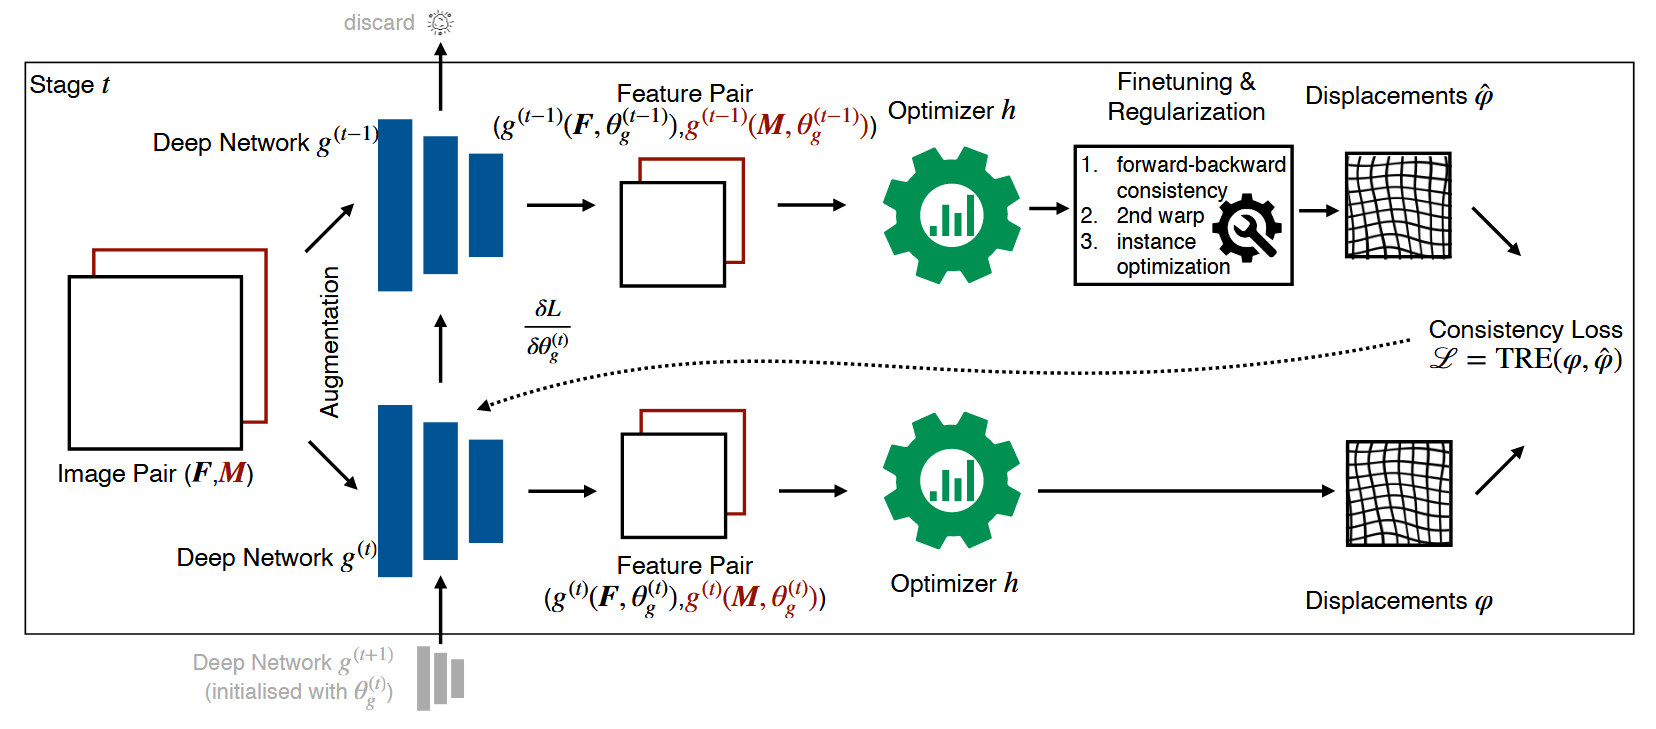
\includegraphics[width=0.9\textwidth]{T_RegCST.png}
  \bicaption[t-fig-c:1]{无监督注册的循环自训练范式概述}{底层配准流水线包括用于特征提取的深度网络g和用于预测位移的可微优化器h。在阶段t,我们使用基于前一阶段网络g(t-1)的特征生成的伪标签来监督网络g(t)的训练。对于最优特征学习,优化器的伪位移被进一步细化和正则化。}{Fig.$\!$ }{Overview of the proposed cyclical self-training paradigm for unsupervised registration. The underlying registration pipeline comprises a deep network for feature extraction g and a differentiable optimizer h to predict the displacements. At stage t, we supervise the training of the network $g^{(t)}$ with pseudo labels generated based on the features from the network $g^{(t-1)}$ from the previous stage. For optimal feature learning, the pseudo displacements from the optimizer are further refined and regularized.}
\end{figure}

\begin{equation}\tag*{(1)}
  f(\boldsymbol{F},\boldsymbol{M};\boldsymbol{\theta}_f)=h(g(\boldsymbol{F},\boldsymbol{M};\boldsymbol{\theta}_g))
\end{equation}

该方法基于我们的一项实证发现:即使使用随机初始化网络$g^{(0)}$(参数为$\theta_G^{(0)}$)提供的随机特征,合适的优化算法$h$仍能预测出合理的初始位移场$\hat{\boldsymbol{\varphi}}^{(0)}$,这与近期关于CNN归纳偏置的研究结论一致[4]。我们利用这些预测位移场作为伪标签来监督自训练的首阶段,通过最小化以下损失函数优化特征提取网络参数$\theta_G^{(1)}$:
\begin{equation}\tag*{(2)}
  \mathcal{L}(\boldsymbol{\theta}_g^{(1)};\mathcal{T})=\frac{1}{|\mathcal{T}|}\sum_i\mathrm{TRE}\left(h\left(g\left(\boldsymbol{F}_i,\boldsymbol{M}_i;\boldsymbol{\theta}_g^{(1)}\right)\right),\hat{\boldsymbol{\varphi}}_i^{(0)}\right)
\end{equation}
其中$\mathrm{TRE}(\hat{\boldsymbol{\varphi}}_\mathrm{i}^{(1)},\hat{\boldsymbol{\varphi}}_\mathrm{i}^{(0)})$表示位移场$\hat{\boldsymbol{\varphi}}_\mathrm{i}^{(1)}$与$\hat{\boldsymbol{\varphi}}_\mathrm{i}^{(0)}$逐元素目标配准误差的均值。

该基础框架存在网络可能过拟合初始伪标签并学习复制随机特征的关键问题。受对比学习最新技术启发[6],我们提出在学习和伪标签生成双路径中引入双重非对称性以增强特征学习效果:首先对双路径输入数据施加不同的随机增强;其次在伪标签路径的优化器后增加(不可微)细调与正则化步骤以提升伪位移场质量(详见第2.3节)。消融实验表明(图2、表1),这两种策略均可有效改善特征学习并强化自我增强效应。

当首阶段自训练收敛后,我们重复该过程$T$次迭代。具体而言,在第$t$阶段:1)使用前一阶段训练网络$g^{(t-1)}$生成精炼伪标签;2)以$g^{(t-1)}$权重初始化当前网络$g^{(t)}$;3)对学习率执行热重启以跳出前一阶段的局部极小值。

\subsection{配准框架}

我们提出的自训练方案是一个灵活、模块化的框架,其独立于输入模态及特征提取器$g$与优化器$h$的具体实现。本节阐述我们在图像和点云配准任务中对$g$和$h$的具体设计选择,其中图像配准为本文主要研究重点。

\textbf{图像配准.} 针对三维输入体数据,我们采用标准3D CNN实现特征提取器$g$。该网络包含六个卷积层,卷积核尺寸为3$\times$3$\times$3,通道数分别为32、64或128。每个卷积层后接批量归一化(BatchNorm)和ReLU激活函数,每隔一个卷积层进行步长为2的下采样,最终获得8倍降采样特征。通过1$\times$1$\times$1卷积将两幅图像特征映射至16维,并输入相关层[21]捕获125个离散位移。

作为优化器,我们基于文献[20]提出的耦合凸优化方法实现三维配准。该方法以固定和移动图像特征为输入,通过最小化平滑性与特征差异的联合目标函数推断位移场。伪标签流中的细化策略包含三个关键要素:1) 前向-后向一致性:额外计算反向位移场($\boldsymbol{F}$到$\boldsymbol{M}$),并通过迭代优化最小化双向场间差异;2) 二次形变:使用当前位移场对移动图像进行形变后重复前述步骤;3) 迭代实例优化:采用Adam算法联合最小化正则化代价与特征差异,对最终位移场进行微调。其中特征差异计算使用第二卷积块后的CNN特征(经1$\times$1$\times$1卷积映射至16通道)。在测试阶段采用相同的细化步骤。

此外,我们提出通过比较网络预测位移与微调后位移的差异来估计训练样本难度。据此实施加权批量采样策略,优先选择场间一致性更高的简单配准对。具体实现中,对所有训练对进行难度排序,并采用参数范围-5至5的sigmoid函数构建加权随机采样器。

\textbf{点云配准.} 对于点云配准任务,我们采用图卷积网络实现特征提取器,并基于文献[9]提出的可微分稀疏循环置信传播算法进行优化。

\section{实验}

\subsection{实验设置}

\textbf{数据集.} 我们在Learn2Reg (L2R)挑战赛[15]的跨患者腹部CT配准数据集上进行主要实验。该数据集包含30例不同患者的三维腹部CT扫描数据,包含13个尺寸差异显著的手动标注解剖结构。原始影像数据与标签来源于[26]。作为L2R基准的一部分,数据经仿射预配准至标准空间,并重采样为统一体素分辨率(2毫米)和空间维度(192$\times$160$\times$256体素)。遵循L2R数据划分方案,使用20例扫描(190对)进行训练,剩余10例(45对)用于评估。数据划分与预处理流程与对比方法[9,27]保持一致。评估指标采用语义标签间的平均Dice相似系数(DSC)及对数雅可比行列式标准差(SDlogJ)。

我们使用DIR-Lab COPDGene数据集[5]进行呼气-吸气相位肺部CT配准的补充实验,该数据集包含10组扫描对。每组扫描提供300个专家标注的解剖标志点用于评估。预处理流程包含:1) 呼气相扫描重采样至1.75$\times$1.00$\times$1.25毫米,吸气相至1.75$\times$1.25$\times$1.75毫米;2) 基于自动生成肺部分割掩膜,截取固定尺寸感兴趣区域(192$\times$192$\times$208体素);3) 对肺部分割结果进行仿射预配准。针对肺部CT关键点配准任务,我们遵循[9]的方法,使用Förstner算法结合非极大值抑制提取CT影像特征点,固定影像约生成1,000个点,移动影像约2,000个点。实验采用五折交叉验证,每折包含8对训练数据和2对测试数据。评估指标为标志点处目标配准误差(TRE)及SDlogJ。

\textbf{实现细节.} 所有方法基于PyTorch框架实现,使用Adam优化器进行网络参数优化。腹部配准任务设置$T$=8个训练阶段,每阶段包含1,000次迭代(batch size=2),学习率采用余弦退火热重启策略,每阶段从$10^{-3}$衰减至$10^{-5}$。超参数根据训练集三个病例的DSC指标确定。肺部配准任务经过$T$=5个阶段(每阶段60个epoch,batch size=4)达到收敛,初始学习率0.001,分别在第40和52 epoch衰减10倍。该任务超参数继承自[9]。两个数据集训练过程均在RTX2080显卡(8GB显存)上完成,耗时约90-100分钟,数据增强采用随机仿射变换。

\subsection{结果}

\textbf{腹部实验.} 首先通过消融实验分析本方法性能。图2展示了多个自训练周期中不同解剖结构类别的配准效果演变,可见各阶段性能持续提升(尤其在早期阶段显著),最终趋于收敛。这验证了伪标签更新与网络训练交替机制产生的自我增强效应。表1上半部分验证了双路径非对称增强(输入增强、伪标签微调)及加权采样策略的有效性,结果表明各组件对实现最优性能均具有重要作用。表1下半部分评估了不同测试配置下的模型表现,结果显示二次形变与Adam微调可带来显著性能提升。

\begin{figure}
  \centering
  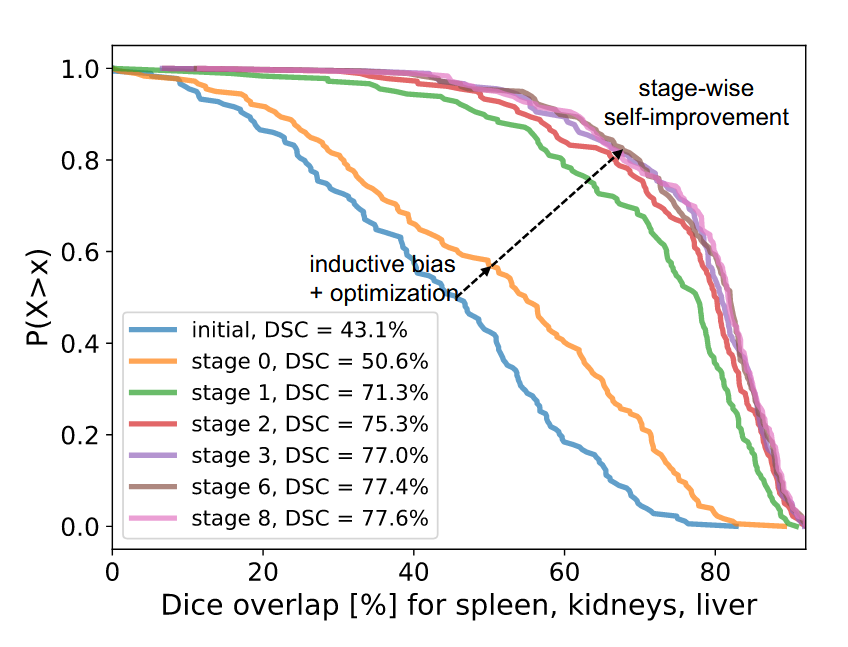
\includegraphics[width=0.9\textwidth]{T_result.png}
  \bicaption[t-fig-c:2]{}{在不同阶段的自我训练后,腹部CT登记的Dice重叠的“相反”累积分布。}{Fig.$\!$ }{“Opposite” cumulative distribution of Dice overlaps for Abdomen CT registration after different stages of self-training.}
\end{figure}

\begin{table}
  \bicaption[t-c:table1]{}{腹部CT配准的消融研究。}{Table$\!$}{Ablation study for abdomen CT registration.}
  \vspace{0.5em}\centering\wuhao
  \begin{tabular}{lcc}
    \toprule
    \textbf{Method}       & \textbf{DSC}  & \textbf{SDlogJ} \\
    \midrule
    prealign              & 25.9          & --              \\
    w/o input augm.       & 48.8          & 0.129           \\
    w/o PL refinement     & 48.8          & 0.200           \\
    w/o weighted sampling & 50.1          & 0.147           \\
    ours                  & 51.1          & 0.146           \\
    \midrule
    1 warp w/o Adam       & 38.6          & 0.061           \\
    1 warp w/ Adam        & 49.6          & 0.119           \\
    2 warps w/o Adam      & 41.1          & 0.088           \\
    2 warps w/Adam (ours) & \textbf{51.1} & 0.146           \\
    \bottomrule
  \end{tabular}
\end{table}

随后,我们将本方法与包括经典算法[1,10,14]和深度学习方法在内的多种最先进无监督方法进行对比,其中深度学习方法涵盖MIND[2,12]/NCC[17]监督训练和对比学习[27]方案。对比数据引自文献[9]与[27]。为直接验证自训练策略优势,我们还使用基于度量的监督方法(MIND[13]、NCC[19])训练了相同框架。实验结果见表2、图3及补充材料图3。本方法在DSC指标上显著超越所有对比方法(对公开代码方法进行Wilcoxon符号秩检验,p<0.0001;SAME方法因未公开代码未参与检验),以51.1\%的DSC刷新当前最佳性能。这证明了新学习范式相较于传统无监督策略的优越性。同时,预测位移场的平滑性指标(SDlogJ)与多数无监督深度方法[2,12]相当,且优于MIND与NCC监督方法。

\begin{figure}
  \centering
  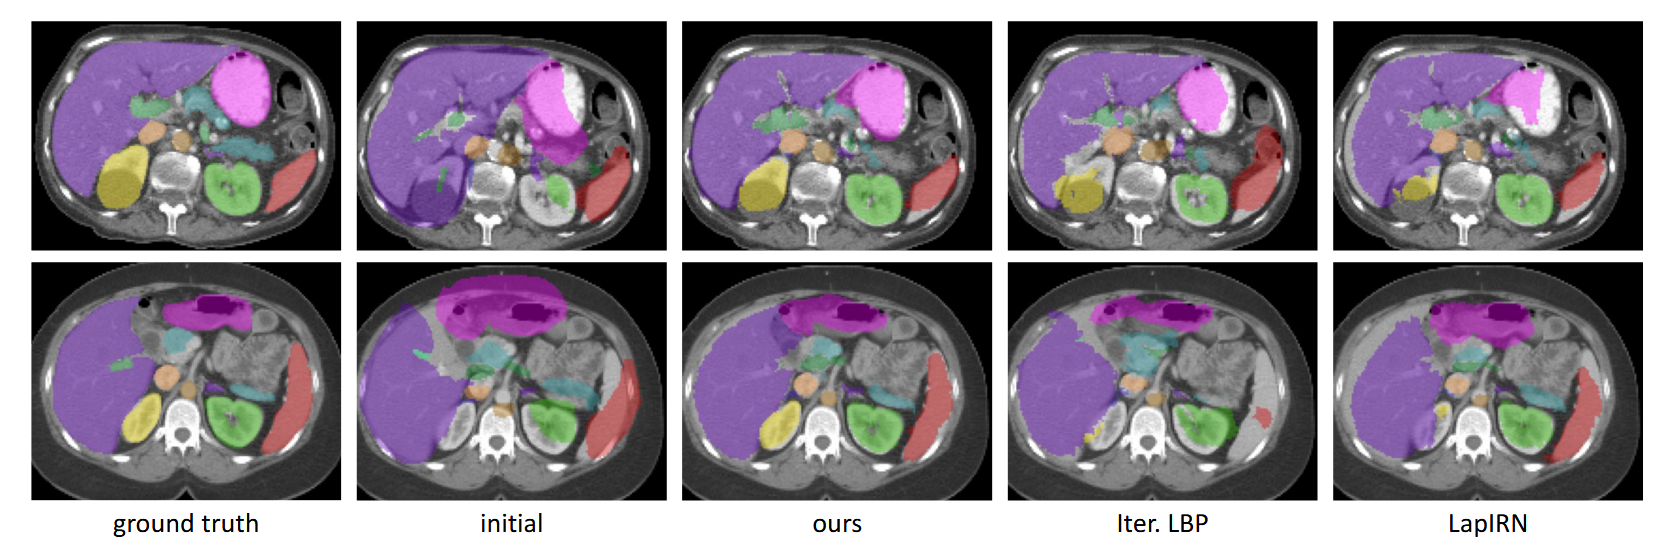
\includegraphics[width=0.9\textwidth]{T_img.png}
  \bicaption[ct-fig:3]{}{所选方法对两例腹部CT数据集(轴向视图)的定性结果。我们展示了扭曲分割标签与固定扫描的叠加}{Fig.$\!$ }{Qualitative results of selected methods on two cases of the Abdomen CT dataset (axial view). We show overlays of the warped segmentation labels with the fixed scan.}
\end{figure}

\begin{table}
  \bicaption[ct:table2]{}{无监督腹部CT配准结果}{Table$\!$}{Results for unsupervised abdomen CT registration.}
  \vspace{0.5em}\centering\wuhao
  \begin{tabular}{lccc}
    \toprule
    \textbf{Method} & \textbf{Dice [\%]} & \textbf{SDlogJ} & \textbf{Time [s]} \\
    \midrule
    pre-aligned     & 25.9               & --              & --                \\
    Adam            & 36.6               & 0.080           & 1.6               \\
    Iter. LBP       & 40.1               & 0.093           & 0.6               \\
    ANTs (SyN)      & 28.4               & {N/A}           & 74.3              \\
    DEEDS           & 46.5               & {N/A}           & 45.4              \\
    \midrule
    VoxelMorph      & 35.4               & 0.134           & 0.2               \\
    PDD             & 41.5               & 0.129           & 1.4               \\
    LapIRN          & 42.4               & 0.089           & 3.8               \\
    SAME            & 49.8               & {N/A}           & 1.2               \\
    \midrule
    MIND sup.       & 47.7               & 0.237           & 1.2               \\
    NCC sup.        & 48.1               & 0.299           & 1.2               \\
    \midrule
    ours            & \textbf{51.1}      & 0.146           & 1.2               \\
    \bottomrule
  \end{tabular}
\end{table}

\textbf{肺部实验.} 在基于点云的肺部配准任务中,我们将循环自训练策略与三种学习方案进行对比:1) 基于人工标注标志点的监督学习[9];2) 结合倒角距离与局部拉普拉斯惩罚的度量监督[23];3) 合成刚性/随机形变场训练。所有策略均基于文献[9]的基准模型实现。此外,我们还对比了三种基于MIND监督的无监督图像配准方法[2,12,17]。表3结果显示,本自训练策略在所有对比方案及现有图像配准SOTA方法中均表现出最优性能。补充材料图4展示了实验的定性结果,可见预测位移场兼具高精度与平滑性,该结论亦得到低SDlogJ值的支持。

\section{结论}

我们提出了一种新型的循环自训练范式用于无监督配准任务。为此,我们开发了模块化的配准流程框架,该框架将深度特征提取网络与可微分优化器相结合,通过正则化与迭代式循环精炼机制,有效稳定了噪声伪标签下的学习过程。相较于依赖浅层特征或图像强度的传统度量监督方法(如NCC、MIND)——这类方法易受噪声干扰并陷入局部极小——我们的优化驱动伪标签监督机制具有显著优势:1)基于优化精炼与正则化的伪标签能够引导网络学习更具噪声鲁棒性的任务相关特征;2)循环学习策略通过渐进式特征增强有效避免局部极小。实验结果表明,本方法在密集图像腹部配准与点云肺部配准任务中均超越当前最先进方法,充分验证了方案的有效性与灵活性。综上所述,本研究不仅首次实现了完全无监督的自训练框架,更为基于学习的无监督配准提供了全新视角。特别值得指出的是,本策略与现有技术(度量监督与对比学习)具有互补性,为未来构建联合训练方案开辟了新可能。

% \title{The title of the English paper}

% \textbf{Abstract:} As one of the most widely used techniques in operations
% research, \emph{ mathematical programming} is defined as a means of maximizing a
% quantity known as \emph{bjective function}, subject to a set of constraints
% represented by equations and inequalities. Some known subtopics of mathematical
% programming are linear programming, nonlinear programming, multiobjective
% programming, goal programming, dynamic programming, and multilevel
% programming$^{[1]}$.

% It is impossible to cover in a single chapter every concept of mathematical
% programming. This chapter introduces only the basic concepts and techniques of
% mathematical programming such that readers gain an understanding of them
% throughout the book$^{[2,3]}$.


% \section{Single-Objective Programming}
% The general form of single-objective programming (SOP) is written
% as follows,
% \begin{equation}\tag*{(123)} % 如果附录中的公式不想让它出现在公式索引中,那就请
%                              % 用 \tag*{xxxx}
% \left\{\begin{array}{l}
% \max \,\,f(x)\\[0.1 cm]
% \mbox{subject to:} \\ [0.1 cm]
% \qquad g_j(x)\le 0,\quad j=1,2,\cdots,p
% \end{array}\right.
% \end{equation}
% which maximizes a real-valued function $f$ of
% $x=(x_1,x_2,\cdots,x_n)$ subject to a set of constraints.

% \newtheorem{mpdef}{Definition}[chapter]
% \begin{mpdef}
% In SOP, we call $x$ a decision vector, and
% $x_1,x_2,\cdots,x_n$ decision variables. The function
% $f$ is called the objective function. The set
% \begin{equation}\tag*{(456)} % 这里同理,其它不再一一指定。
% S=\left\{x\in\Re^n\bigm|g_j(x)\le 0,\,j=1,2,\cdots,p\right\}
% \end{equation}
% is called the feasible set. An element $x$ in $S$ is called a
% feasible solution.
% \end{mpdef}

% \newtheorem{mpdefop}[mpdef]{Definition}
% \begin{mpdefop}
% A feasible solution $x^*$ is called the optimal
% solution of SOP if and only if
% \begin{equation}
% f(x^*)\ge f(x)
% \end{equation}
% for any feasible solution $x$.
% \end{mpdefop}

% One of the outstanding contributions to mathematical programming was known as
% the Kuhn-Tucker conditions\ref{eq:ktc}. In order to introduce them, let us give
% some definitions. An inequality constraint $g_j(x)\le 0$ is said to be active at
% a point $x^*$ if $g_j(x^*)=0$. A point $x^*$ satisfying $g_j(x^*)\le 0$ is said
% to be regular if the gradient vectors $\nabla g_j(x)$ of all active constraints
% are linearly independent.

% Let $x^*$ be a regular point of the constraints of SOP and assume that all the
% functions $f(x)$ and $g_j(x),j=1,2,\cdots,p$ are differentiable. If $x^*$ is a
% local optimal solution, then there exist Lagrange multipliers
% $\lambda_j,j=1,2,\cdots,p$ such that the following Kuhn-Tucker conditions hold,
% \begin{equation}
% \label{eq:ktc}
% \left\{\begin{array}{l}
%     \nabla f(x^*)-\sum\limits_{j=1}^p\lambda_j\nabla g_j(x^*)=0\\[0.3cm]
%     \lambda_jg_j(x^*)=0,\quad j=1,2,\cdots,p\\[0.2cm]
%     \lambda_j\ge 0,\quad j=1,2,\cdots,p.
% \end{array}\right.
% \end{equation}
% If all the functions $f(x)$ and $g_j(x),j=1,2,\cdots,p$ are convex and
% differentiable, and the point $x^*$ satisfies the Kuhn-Tucker conditions
% (\ref{eq:ktc}), then it has been proved that the point $x^*$ is a global optimal
% solution of SOP.

% \subsection{Linear Programming}
% \label{sec:lp}

% If the functions $f(x),g_j(x),j=1,2,\cdots,p$ are all linear, then SOP is called
% a {\em linear programming}.

% The feasible set of linear is always convex. A point $x$ is called an extreme
% point of convex set $S$ if $x\in S$ and $x$ cannot be expressed as a convex
% combination of two points in $S$. It has been shown that the optimal solution to
% linear programming corresponds to an extreme point of its feasible set provided
% that the feasible set $S$ is bounded. This fact is the basis of the {\em simplex
%   algorithm} which was developed by Dantzig as a very efficient method for
% solving linear programming.
% \begin{table}[ht]
% \centering
%   \centering
%   \caption*{Table~1\hskip1em This is an example for manually numbered table, which
%     would not appear in the list of tables}
%   \label{tab:badtabular2}
%   \begin{tabular}[c]{|m{1.5cm}|c|c|c|c|c|c|}\hline
%     \multicolumn{2}{|c|}{Network Topology} & \# of nodes &
%     \multicolumn{3}{c|}{\# of clients} & Server \\\hline
%     GT-ITM & Waxman Transit-Stub & 600 &
%     \multirow{2}{2em}{2\%}&
%     \multirow{2}{2em}{10\%}&
%     \multirow{2}{2em}{50\%}&
%     \multirow{2}{1.2in}{Max. Connectivity}\\\cline{1-3}
%     \multicolumn{2}{|c|}{Inet-2.1} & 6000 & & & &\\\hline
%     & \multicolumn{2}{c|}{ABCDEF} &\multicolumn{4}{c|}{} \\\hline
% \end{tabular}
% \end{table}

% Roughly speaking, the simplex algorithm examines only the extreme points of the
% feasible set, rather than all feasible points. At first, the simplex algorithm
% selects an extreme point as the initial point. The successive extreme point is
% selected so as to improve the objective function value. The procedure is
% repeated until no improvement in objective function value can be made. The last
% extreme point is the optimal solution.

% \subsection{Nonlinear Programming}

% If at least one of the functions $f(x),g_j(x),j=1,2,\cdots,p$ is nonlinear, then
% SOP is called a {\em nonlinear programming}.

% A large number of classical optimization methods have been developed to treat
% special-structural nonlinear programming based on the mathematical theory
% concerned with analyzing the structure of problems.

% Now we consider a nonlinear programming which is confronted solely with
% maximizing a real-valued function with domain $\Re^n$.  Whether derivatives are
% available or not, the usual strategy is first to select a point in $\Re^n$ which
% is thought to be the most likely place where the maximum exists. If there is no
% information available on which to base such a selection, a point is chosen at
% random. From this first point an attempt is made to construct a sequence of
% points, each of which yields an improved objective function value over its
% predecessor. The next point to be added to the sequence is chosen by analyzing
% the behavior of the function at the previous points. This construction continues
% until some termination criterion is met. Methods based upon this strategy are
% called {\em ascent methods}, which can be classified as {\em direct methods},
% {\em gradient methods}, and {\em Hessian methods} according to the information
% about the behavior of objective function $f$. Direct methods require only that
% the function can be evaluated at each point. Gradient methods require the
% evaluation of first derivatives of $f$. Hessian methods require the evaluation
% of second derivatives. In fact, there is no superior method for all
% problems. The efficiency of a method is very much dependent upon the objective
% function.

% \subsection{Integer Programming}

% {\em Integer programming} is a special mathematical programming in which all of
% the variables are assumed to be only integer values. When there are not only
% integer variables but also conventional continuous variables, we call it {\em
%   mixed integer programming}. If all the variables are assumed either 0 or 1,
% then the problem is termed a {\em zero-one programming}. Although integer
% programming can be solved by an {\em exhaustive enumeration} theoretically, it
% is impractical to solve realistically sized integer programming problems. The
% most successful algorithm so far found to solve integer programming is called
% the {\em branch-and-bound enumeration} developed by Balas (1965) and Dakin
% (1965). The other technique to integer programming is the {\em cutting plane
%   method} developed by Gomory (1959).

% \hfill\textit{Uncertain Programming\/}\quad(\textsl{BaoDing Liu, 2006.2})

% \section*{References}
% \noindent{\itshape NOTE: These references are only for demonstration. They are
%   not real citations in the original text.}

% \begin{translationbib}
% \item Donald E. Knuth. The \TeX book. Addison-Wesley, 1984. ISBN: 0-201-13448-9
% \item Paul W. Abrahams, Karl Berry and Kathryn A. Hargreaves. \TeX\ for the
%   Impatient. Addison-Wesley, 1990. ISBN: 0-201-51375-7
% \item David Salomon. The advanced \TeX book.  New York : Springer, 1995. ISBN:0-387-94556-3
% \end{translationbib}

% \chapter{外文资料的调研阅读报告或书面翻译}

% \title{英文资料的中文标题}

% {\heiti 摘要:} 本章为外文资料翻译内容。如果有摘要可以直接写上来,这部分好像没有
% 明确的规定。

% \section{单目标规划}
% 北冥有鱼,其名为鲲。鲲之大,不知其几千里也。化而为鸟,其名为鹏。鹏之背,不知其几
% 千里也。怒而飞,其翼若垂天之云。是鸟也,海运则将徙于南冥。南冥者,天池也。
% \begin{equation}\tag*{(123)}
%  p(y|\mathbf{x}) = \frac{p(\mathbf{x},y)}{p(\mathbf{x})}=
% \frac{p(\mathbf{x}|y)p(y)}{p(\mathbf{x})}
% \end{equation}

% 吾生也有涯,而知也无涯。以有涯随无涯,殆已!已而为知者,殆而已矣!为善无近名,为
% 恶无近刑,缘督以为经,可以保身,可以全生,可以养亲,可以尽年。

% \subsection{线性规划}
% 庖丁为文惠君解牛,手之所触,肩之所倚,足之所履,膝之所倚,砉然响然,奏刀騞然,莫
% 不中音,合于桑林之舞,乃中经首之会。
% \begin{table}[ht]
% \centering
%   \centering
%   \caption*{表~1\hskip1em 这是手动编号但不出现在索引中的一个表格例子}
%   \label{tab:badtabular3}
%   \begin{tabular}[c]{|m{1.5cm}|c|c|c|c|c|c|}\hline
%     \multicolumn{2}{|c|}{Network Topology} & \# of nodes &
%     \multicolumn{3}{c|}{\# of clients} & Server \\\hline
%     GT-ITM & Waxman Transit-Stub & 600 &
%     \multirow{2}{2em}{2\%}&
%     \multirow{2}{2em}{10\%}&
%     \multirow{2}{2em}{50\%}&
%     \multirow{2}{1.2in}{Max. Connectivity}\\\cline{1-3}
%     \multicolumn{2}{|c|}{Inet-2.1} & 6000 & & & &\\\hline
%     & \multicolumn{2}{c|}{ABCDEF} &\multicolumn{4}{c|}{} \\\hline
% \end{tabular}
% \end{table}

% 文惠君曰:“嘻,善哉!技盖至此乎?”庖丁释刀对曰:“臣之所好者道也,进乎技矣。始臣之
% 解牛之时,所见无非全牛者;三年之后,未尝见全牛也;方今之时,臣以神遇而不以目视,
% 官知止而神欲行。依乎天理,批大郤,导大窾,因其固然。技经肯綮之未尝,而况大坬乎!
% 良庖岁更刀,割也;族庖月更刀,折也;今臣之刀十九年矣,所解数千牛矣,而刀刃若新发
% 于硎。彼节者有间而刀刃者无厚,以无厚入有间,恢恢乎其于游刃必有余地矣。是以十九年
% 而刀刃若新发于硎。虽然,每至于族,吾见其难为,怵然为戒,视为止,行为迟,动刀甚微,
% 謋然已解,如土委地。提刀而立,为之而四顾,为之踌躇满志,善刀而藏之。”

% 文惠君曰:“善哉!吾闻庖丁之言,得养生焉。”


% \subsection{非线性规划}
% 孔子与柳下季为友,柳下季之弟名曰盗跖。盗跖从卒九千人,横行天下,侵暴诸侯。穴室枢
% 户,驱人牛马,取人妇女。贪得忘亲,不顾父母兄弟,不祭先祖。所过之邑,大国守城,小
% 国入保,万民苦之。孔子谓柳下季曰:“夫为人父者,必能诏其子;为人兄者,必能教其弟。
% 若父不能诏其子,兄不能教其弟,则无贵父子兄弟之亲矣。今先生,世之才士也,弟为盗
% 跖,为天下害,而弗能教也,丘窃为先生羞之。丘请为先生往说之。”

% 柳下季曰:“先生言为人父者必能诏其子,为人兄者必能教其弟,若子不听父之诏,弟不受
% 兄之教,虽今先生之辩,将奈之何哉?且跖之为人也,心如涌泉,意如飘风,强足以距敌,
% 辩足以饰非。顺其心则喜,逆其心则怒,易辱人以言。先生必无往。”

% 孔子不听,颜回为驭,子贡为右,往见盗跖。

% \subsection{整数规划}
% 盗跖乃方休卒徒大山之阳,脍人肝而餔之。孔子下车而前,见谒者曰:“鲁人孔丘,闻将军
% 高义,敬再拜谒者。”谒者入通。盗跖闻之大怒,目如明星,发上指冠,曰:“此夫鲁国之
% 巧伪人孔丘非邪?为我告之:尔作言造语,妄称文、武,冠枝木之冠,带死牛之胁,多辞缪
% 说,不耕而食,不织而衣,摇唇鼓舌,擅生是非,以迷天下之主,使天下学士不反其本,妄
% 作孝弟,而侥幸于封侯富贵者也。子之罪大极重,疾走归!不然,我将以子肝益昼餔之膳。”


% \chapter{其它附录}
% 前面两个附录主要是给本科生做例子。其它附录的内容可以放到这里,当然如果你愿意,可
% 以把这部分也放到独立的文件中,然后将其到主文件中。
%本科生翻译论文
\end{appendix}
%%%%%%%%%%%%%%%%%%%%%%%%%%%%%%%%%%%%%%%%%%%%%%%%%%%%%%%%%%%%%%%%%%%%%%%%%%%%%%%%
% 本科书序(威海校区)
%%%%%%%%%%%%%%%%%%%%%%%%%%%%%%%%%%%%%%%%%%%%%%%%%%%%%%%%%%%%%%%%%%%%%%%%%%%%%%%%
% \authorization %授权
% % \authorization[scan.pdf] %添加扫描页的命令,与上互斥
% \bibliography{reference} % 参考文献
% % !Mode:: "TeX:UTF-8"
\begin{acknowledgements}

在我完成本论文之际,心中感慨万千,衷心感谢在这段旅程中给予我支持与帮助的人们。首先,我要特别感谢我的指导老师骆功宁教授。您以渊博的知识和严谨的治学态度,给予我悉心的指导和耐心的教诲。在整个毕设过程中,您不仅为我指明了研究的方向,更以您的严谨与热情感染了我,让我在困惑与迷茫中找到了前进的动力。每一次的讨论与交流,都让我豁然开朗,能够顺利完成论文,离不开您的辛勤付出。

同时,我也要感谢我的同学们。在这段重要的时光里,大家的支持与帮助让我倍感温暖。在无数个深夜的图书馆学习时光中,我们相互鼓励,分享经验,共同克服各种困难。无论是对论文的讨论,还是对生活的倾诉,都是我大学生活中的美好瞬间。你们的陪伴,让我在求学路上不再孤单,成为我最宝贵的财富。

此外,我非常感谢我的家人。你们无条件的支持与理解,是我在追求学术道路上最大的动力。在我遇到困难时,你们给予我温暖的鼓励,始终相信我、支持我,帮助我渡过一个又一个难关。感恩有你们的陪伴,才让我拥有了克服挑战的勇气与信心。

我也要感谢验收时各位老师对我论文格式和内容的指导,您们的专业意见与建议使我的论文更加完善。每一位老师的认真审阅和点评都让我获益匪浅,您的严谨与负责让我明白了学术研究的严肃性,也让我学会了在不断修正中追求卓越。

历历浮生,无非败而后成。回首大学四年,我经历了学习的高峰与低谷,收获了知识与友谊,更锻炼了自己的意志与品格。每一个坚持的时刻都在教会我,持之以恒的努力终会迎来丰硕的成果。感谢我自己在这条道路上的坚持与努力,没有放弃,是我走到今天的重要原因。未来的路依然漫长,我会带着这份感恩与勇气,继续前行。

衷心感谢每一位在我人生旅程中给予我帮助的人,愿我们都能在各自的领域中,不断追求卓越,共同成就美好的未来。


\end{acknowledgements}
 %致谢
% \begin{appendix}%附录
% 

\chapter{外文资料原文}
\label{cha:engorg}

\title{Unsupervised 3D registration through optimization-guided cyclical self-training}

\textbf{Abstract:}State-of-the-art deep learning-based registration methods employ three different learning strategies: supervised learning, which requires costly manual annotations, unsupervised learning, which heavily relies on hand-crafted similarity metrics designed by domain experts, or learning from synthetic data, which introduces a domain shift. To overcome the limitations of these strategies, we propose a novel selfsupervised learning paradigm for unsupervised registration, relying on self-training. Our idea is based on two key insights. Feature-based differentiable optimizers 1) perform reasonable registration even from random features and 2) stabilize the training of the preceding feature extraction network on noisy labels. Consequently, we propose cyclical self-training, where pseudo labels are initialized as the displacement fields inferred from random features and cyclically updated based on more and more expressive features from the learning feature extractor, yielding a selfreinforcement effect. We evaluate the method for abdomen and lung registration, consistently surpassing metric-based supervision and outperforming diverse state-of-the-art competitors. Source code is available at https://github.com/multimodallearning/reg-cyclical-self-train.

\section{Introduction}

Medical image registration is a fundamental task in medical imaging with applications ranging from multi-modal data fusion to temporal data analysis. In recent years, deep learning has advanced learning-based registration methods [11], which achieve competitive performances at low runtimes and thus constitute a promising alternative to accurate but slow classical optimization methods. A decisive factor in successfully training deep learning-based methods is the choice of a suitable strategy to supervise the learning process. In the literature, there exist three different learning strategies. The first is supervised learning based on manual annotations such as landmark correspondences [9] or semantic labels [16]. However, manual annotations are costly and may introduce a label bias [2]. Alternatively, a second strategy employs synthetic deformation fields to generate image pairs with precisely known displacement fields [7]. However, this introduces a domain gap between synthetic training and real test pairs, limiting the performance at inference time. Elaborated deformation techniques can reduce the gap but require strong domain knowledge, are tailored to specific problems, and do not generalize across tasks. The third widely used training strategy is unsupervised metric-based learning, maximizing a similarity metric between fixed and warped moving images, e.g. implemented in [2,17]. Popular metrics include normalized cross-correlation [19] and MIND [13]. However, the success of this strategy strongly depends on the specific hand-crafted metric, and the performance of the trained deep learning models is often inferior to a classical optimization-based counterpart. Considering the deficiencies of the above training techniques, in this work, we introduce a novel learning strategy for unsupervised registration based on the concept of self-training. Self-training is a widespread training strategy for semi-supervised learning [24] and domain adaptation [29]. The core idea is to pre-train a network on available labeled data and subsequently apply the model to the unlabeled data to generate so-called pseudo labels. Afterwards, one alternates between re-training the model on the union of labeled and pseudo-labeled data and updating the pseudo labels with the current model. This general concept was successfully adapted to diverse tasks and settings, with methods in medical context primarily focusing on segmentation [8,18]. These methods resort to a special form of self-training, the Mean Teacher paradigm [22], where pseudo labels are continuously provided by a teacher model, representing a temporal ensemble of the learning network. A persistent problem of classical and Mean Teacher-based selftraining is the inherent noise of the pseudo labels, which can severely hamper the learning process. As a remedy, some works aim to filter reliable pseudo labels based on model uncertainty [28]. Only recently, the Mean Teacher was adapted to the registration problem, tackling domain adaptation [3] or complementing metric-based supervision for adaptive regularization weighting [25]. Contrary to these methods, we introduce self-training for registration in a fully unsupervised setting, with pseudo labels as the single source of supervision.

\textbf{Contributions.}

We introduce a novel learning paradigm for unsupervised registration by adapting the concept of self-training to the problem. This involves two principal challenges. First, labeled data for the pre-training stage is unavailable, raising the question of how to generate initial pseudo labels. Second, as a general problem in self-training, the negative impact of noise in the pseudo labels needs to be mitigated. In our pursuit to overcome these challenges, we made two decisive observations (see Fig.2) when exploring a combination of deep learning-based feature extraction with differentiable optimization algorithms for the displacement prediction, such as [9,20]. First, we found that feature-based optimizers predict reasonable displacement fields and improve the initial registration even when applied to the output of random feature networks (orange line in Fig.2). We attribute this feature to the inductive bias of deep neural networks, which extract somewhat useful features even with random weights [4]. These predicted displacements thus constitute meaningful initial pseudo labels, solving the first problem and leaving us with the second problem to overcome the noise in the labels. In this context, we made the second observation that the intrinsic regularizing capacity of the optimizers stabilizes the learning from noisy labels. Specifically, training the feature extractor on our initial pseudo labels yielded registrations surpassing the accuracy of the noisy labels used for training (green, red, purple, brown, and magenta lines in Fig.2). Consequently, we propose a cyclical self-training scheme, alternating between training the feature extractor and updating the pseudo labels. As such, our novel learning paradigm does not require costly manual annotations, prevents the domain shift of synthetic deformations, and is independent of hand-crafted similarity metrics. Moreover, our method significantly differs from previous uncertainty-based pseudo label filtering strategies since it implicitly overcomes the negative impact of noisy labels by combining deep feature learning with regularizing differentiable optimization. We evaluate the method for CT abdomen registration and keypoint-based lung registration, demonstrating substantial improvements over diverse state-of-theart comparison methods.

\section{Methods}

\subsection{Problem setup}

Given a data pair ($F$,$M$) of a fixed and a moving image as input, registration aims at finding a displacement field $\varphi$ that spatially aligns $M$ to $F$ . We address the task in an unsupervised setting, where training data $\mathcal{T}=\{(\boldsymbol{F}_i,\boldsymbol{M}_i)\}_{i=1}^{|\mathcal{T}|}$  consists of $|\mathcal{T}|$ unlabeled data pairs. Given the training data, we aim to learn a function $f$ with parameters $\theta_f$ , (partially) represented by a deep network, which predicts displacement fields as $ \hat{\boldsymbol{\varphi}}=f(\boldsymbol{F},\boldsymbol{M};\boldsymbol{\theta}_f)$.

\subsection{Cyclical self-training}

We propose to solve the above problem with a cyclical self-training strategy visualized in Fig.1. While existing self-training methods assume the availability of some labeled data, annotations are unavailable in our unsupervised setting. To overcome this issue and generate an initial set of pseudo labels for the first stage of self-training, we parameterize the function $f$ as the combination of a deep neural network $g$ for feature extraction with a non-learnable but differentiable feature-based optimization algorithm $h$ for displacement prediction, i.e.

\begin{figure}
  \centering
  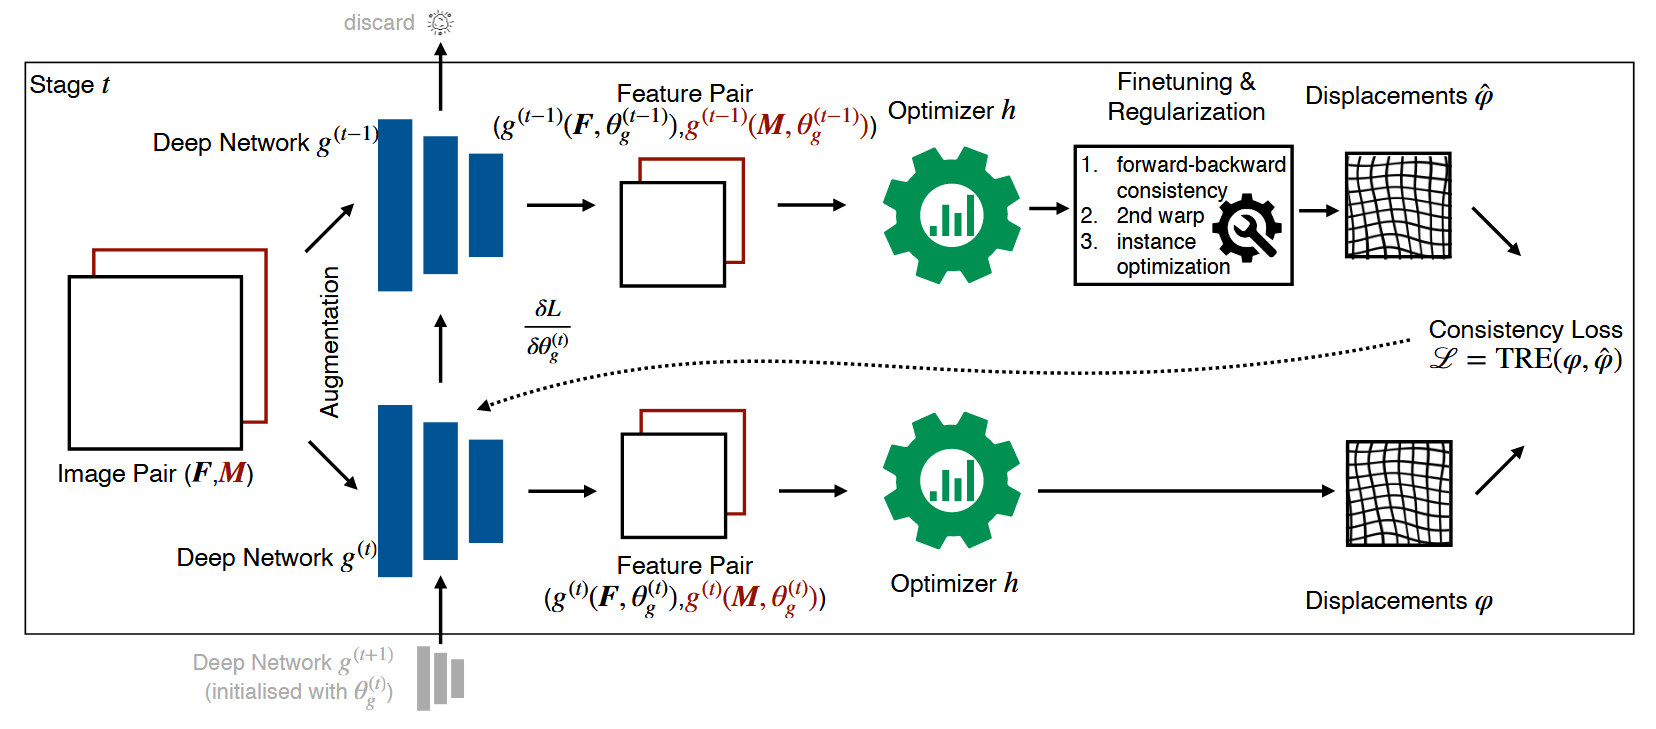
\includegraphics[width=0.9\textwidth]{T_RegCST.png}
  \bicaption[t-fig:1]{无监督注册的循环自训练范式概述}{底层配准流水线包括用于特征提取的深度网络g和用于预测位移的可微优化器h。在阶段t,我们使用基于前一阶段网络g(t-1)的特征生成的伪标签来监督网络g(t)的训练。对于最优特征学习,优化器的伪位移被进一步细化和正则化。}{Fig.$\!$ }{Overview of the proposed cyclical self-training paradigm for unsupervised registration. The underlying registration pipeline comprises a deep network for feature extraction g and a differentiable optimizer h to predict the displacements. At stage t, we supervise the training of the network $g^{(t)}$ with pseudo labels generated based on the features from the network $g^{(t-1)}$ from the previous stage. For optimal feature learning, the pseudo displacements from the optimizer are further refined and regularized.}
\end{figure}

\begin{equation}\tag*{(1)}
  f(\boldsymbol{F},\boldsymbol{M};\boldsymbol{\theta}_f)=h(g(\boldsymbol{F},\boldsymbol{M};\boldsymbol{\theta}_g))
\end{equation}

The approach is based on our empirical observation that a suitable optimization algorithm $h$ can predict reasonable initial displacement fields $\hat{\boldsymbol{\varphi}}^{(0)}$ from random features provided by a network $g^{(0)}$ with random initialization$\theta_G^{(0)} $, which is in line with recent studies on the inductive bias of CNNs [4]. We leverage these predicted displacements as pseudo labels to supervise the first stage of self-training,where the parameters of the feature extractor with different initialization$\theta_G^{(1)} $are optimized by minimizing the loss

\begin{equation}\tag*{(2)}
  \mathcal{L}(\boldsymbol{\theta}_g^{(1)};\mathcal{T})=\frac{1}{|\mathcal{T}|}\sum_i\mathrm{TRE}\left(h\left(g\left(\boldsymbol{F}_i,\boldsymbol{M}_i;\boldsymbol{\theta}_g^{(1)}\right)\right),\hat{\boldsymbol{\varphi}}_i^{(0)}\right)
\end{equation}

with $\mathrm{TRE}(\hat{\boldsymbol{\varphi}}_\mathrm{i}^{(1)},\hat{\boldsymbol{\varphi}}_\mathrm{i}^{(0)})$ denoting the mean over the element-wise target registration error between the displacement fields $\hat{\boldsymbol{\varphi}}_\mathrm{i}^{(1)} $ and $\hat{\boldsymbol{\varphi}}_\mathrm{i}^{(0)}$.

A critical problem of this basic setup is that the network might overfit the initial pseudo labels and learn to reproduce random features. Therefore, in the spirit of recent techniques from contrastive learning [6], we propose to improve the efficacy of feature learning by incorporating asymmetries into the learning and pseudo label streams at two levels. First, we apply different random augmentations to the input pairs in both streams. Second, we augment the pseudo label stream with additional (non-differentiable) fine-tuning and regularization steps after the optimizer to improve the pseudo displacement fields (see Sec. 2.3 for details). As demonstrated in our ablation experiments (Fig.2, Tab.1), both strategies improve feature learning and strengthen the self-improvement effect.

Once the first stage of self-training has converged, we repeat the process $T$ times. Specifically, at stage $t$, we generate refined pseudo labels with the trained network $g^{(t-1)}$ from the previous stage, initialize the learning network $g^{(t)}$ with the weights from $g^{(t-1)}$ and perform a warm restart on the learning rate to escape potential local minima from the previous stage.

\subsection{Registration framework}

Our proposed self-training scheme is a flexible, modular framework, agnostic to the input modality and the specific implementation of feature extractor $g$ and optimizer $h$. This section describes our specific design choices for $g$ and $h$ for image and point cloud registration, with the former being our main focus.


\textbf{Image registration.} To extract features from 3D input volumes, we implement g a standard 3D CNN with six convolution layers with kernel sizes 3 $\times$ 3 $\times$ 3 and 32, 64, or 128 channels. Each convolution is followed by BatchNorm and ReLU, and every second convolution contains a stride of 2, yielding a downsampling factor of 8. The outputs for both images are mapped to 16-dimensional features using a 1 $\times$ 1 $\times$ 1 convolution and fed into a correlation layer [21] that captures 125 discrete displacements.

As the optimizer, we adapt the coupled convex optimization for learningbased 3D registration from [20], which, given fixed and moving features, infers a displacement field that minimizes a combined objective of smoothness and feature dissimilarity. Our proposed refinement strategy in the pseudo label stream comprises three ingredients. 1) Forward-backward consistency additionally computes the reverse displacement field ($\boldsymbol{F}$ to $\boldsymbol{M}$ ) and then iteratively minimizes the discrepancy between both fields. 2) For a second warp, the moving image is warped with the inferred displacement field before repeating all previous steps. 3) Iterative instance optimization finetunes the final displacement field with Adam by jointly minimizing regularization cost and feature dissimilarity. For the latter, we use the CNN features after the second convolution block and map them with a 1$\times$1$\times$1 convolution to 16 channels. We apply the same refinement steps at test time. Moreover, we propose to leverage the difference between network-predicted and finetuned displacements to estimate the difficulty of the training samples. Consequently, we apply a weighted batch sampling at training that increases the probability of using less difficult registration pairs with a higher agreement between both fields. We rank all training pairs and use a sigmoid function with arguments ranging linearly from -5 to 5 for the weighted random sampler.

\textbf{Point cloud registration.} For point cloud registration, we implement the feature extractor as a graph CNN and rely on sparse loopy belief propagation for differentiable optimization, as introduced in [9].

\section{Experiments}

\subsection{Experimental setup}

\textbf{Datasets.} We conduct our main experiments for inter-patient abdomen CT registration using the corresponding dataset of the Learn2Reg (L2R) Challenge [15]. The dataset contains 30 abdominal 3D CT scans of different patients with 13 manually labeled anatomical structures of strongly varying sizes. The original image data and labels are from [26]. As part of L2R, they were affinely preregistered into a canonical space and resampled to identical voxel resolutions (2 mm) and spatial dimensions (192 $\times$ 160 $\times$ 256 vx). Following the data split of L2R, we use 20 scans (190 pairs) for training and the remaining 10 scans (45 pairs) for evaluation. Hence, data split and preprocessing are consistent with compared previous works [9,27]. As metrics, we report the mean Dice overlap (DSC) between the semantic labels and the standard deviation of the logarithmic Jacobian determinant (SDlogJ).

We perform a second experiment for inhale-to-exhale lung CT registration on the DIR-Lab COPDGene dataset5 [5], which comprises 10 such scan pairs. For each pair, 300 expert-annotated landmark correspondences are available for evaluation. We pre-process all scans in multiple steps: 1) resampling to 1.75$\times$1.00$\times$1.25 mm for exhale and 1.75$\times$1.25$\times$1.75 mm for inhale, 2) cropping with fixed-size bounding boxes (192 $\times$ 192 $\times$ 208 vx), centered around automatically generated lung masks, 3) affine pre-registration, aligning the lung masks. Since we focus on keypoint-based registration of the lung CTs, we follow [9] and extract distinctive keypoints from the CTs using the Förstner algorithm with non-maximum suppression, yielding around 1k points in the fixed and 2k points in the moving cloud. In our experiments, we perform 5-fold cross-validation, with each fold comprising eight data pairs for training and two for testing. We report the target registration error (TRE) at the landmarks and the SDlogJ as metrics.

\textbf{Implementation details.} We implement all methods in Pytorch and optimize network parameters with the Adam optimizer. For abdomen registration, we train for $T$ = 8 stages, each stage comprising 1000 iterations with a batch size of 2. The learning rate follows a cosine annealing warm restart schedule, decaying from $10^{-3}$ to $10^{-5}$ at each stage. Hyper-parameters were set based on the DSC on three cases from the training set. For lung registration, the model converged after $T$ = 5 stages of 60 epochs with batch size 4, with an initial learning rate of 0.001, decreased by a factor of 10 at epochs 40 and 52. Here, hyper-parameters were adopted from [9]. For both datasets, training requires 90-100 min and 8 GB on an RTX2080, and input augmentations consist of random affine transformations.

\subsection{Results}

\textbf{Abdomen. }First, we analyze our method in several ablation experiments. In Fig.2, we visualize the performance of our method on a subset of classes over several cycles of self-training. We observe consistent improvements over the stages, particularly pronounced at early stages while the performance converges later on. This highlights the self-reinforcing effect achieved through alternating pseudo label updates and network training. In the upper part of Tab.1, we verify the efficacy of incorporating asymmetries (input augmentations, finetuning of pseudo labels) into both streams and weighted sampling. The results confirm the importance of each component to reach optimal performance. In the lower part of Tab.1, we evaluate our final model under different test configurations, highlighting the improvements through a second warp and Adam finetuning.

\begin{figure}
  \centering
  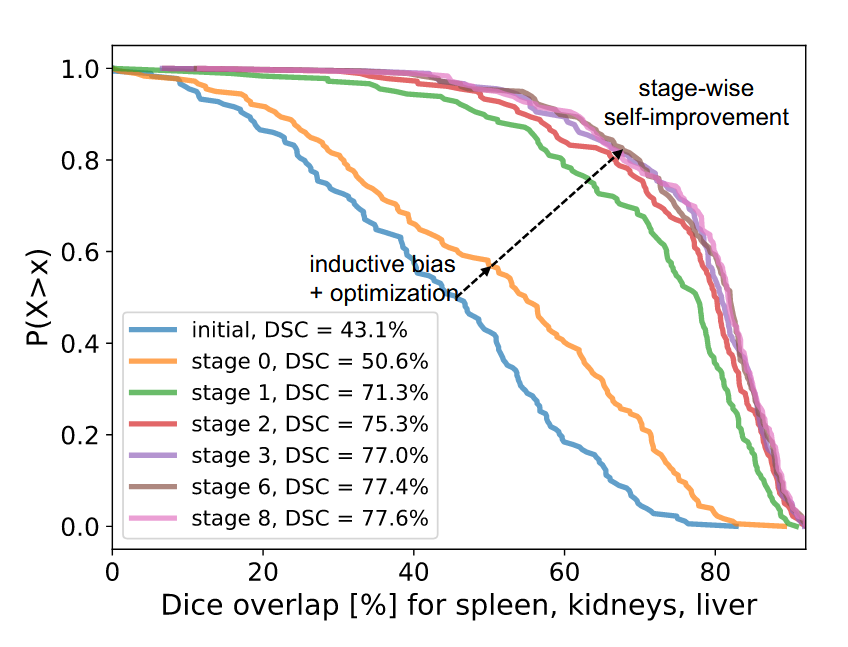
\includegraphics[width=0.9\textwidth]{T_result.png}
  \bicaption[t-fig:2]{}{在不同阶段的自我训练后,腹部CT登记的Dice重叠的“相反”累积分布。}{Fig.$\!$ }{“Opposite” cumulative distribution of Dice overlaps for Abdomen CT registration after different stages of self-training.}
\end{figure}

\begin{table}
  \bicaption[t:table1]{}{腹部CT配准的消融研究。}{Table$\!$}{Ablation study for abdomen CT registration.}
  \vspace{0.5em}\centering\wuhao
  \begin{tabular}{lcc}
    \toprule
    \textbf{Method}       & \textbf{DSC}  & \textbf{SDlogJ} \\
    \midrule
    prealign              & 25.9          & --              \\
    w/o input augm.       & 48.8          & 0.129           \\
    w/o PL refinement     & 48.8          & 0.200           \\
    w/o weighted sampling & 50.1          & 0.147           \\
    ours                  & 51.1          & 0.146           \\
    \midrule
    1 warp w/o Adam       & 38.6          & 0.061           \\
    1 warp w/ Adam        & 49.6          & 0.119           \\
    2 warps w/o Adam      & 41.1          & 0.088           \\
    2 warps w/Adam (ours) & \textbf{51.1} & 0.146           \\
    \bottomrule
  \end{tabular}
\end{table}

Next, we compare our method to a comprehensive set of state-of-the-art unsupervised methods, including classical algorithms [1,10,14] and deep learningbased approaches, trained with MIND [2,12]/NCC [17] supervision or contrastive learning [27]. The results are collected from [9] and [27]. Moreover, we train our own registration framework with metric-based supervision (MIND [13], NCC [19]) to directly verify the advantage of our self-training strategy. Results are shown in Tab.2, Fig.3, and Supp., Fig.3. Our method substantially outperforms all comparison methods in terms of DSC (statistical significance is confirmed by a Wilcoxon-signed rank test with p<0.0001 for all competitors with public code, which excludes SAME) and sets a new state-of-the-art accuracy of 51.1\% DSC. This highlights the advantages of our new learning paradigm over previous unsupervised strategies. Meanwhile, the smoothness of predicted displacement fields (SDlogJ) is comparable with most unsupervised deep learning-based methods [2,12] and superior to MIND- and NCC-supervision.

\begin{figure}
  \centering
  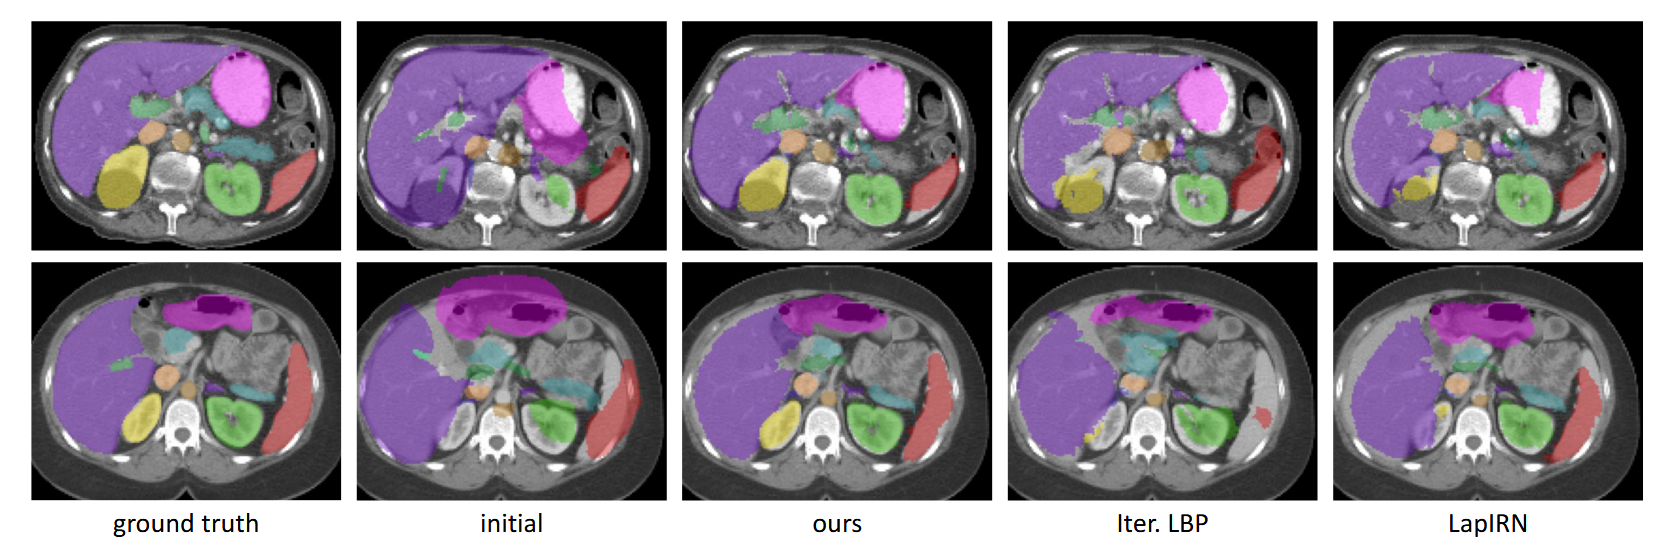
\includegraphics[width=0.9\textwidth]{T_img.png}
  \bicaption[t-fig:3]{}{所选方法对两例腹部CT数据集(轴向视图)的定性结果。我们展示了扭曲分割标签与固定扫描的叠加}{Fig.$\!$ }{Qualitative results of selected methods on two cases of the Abdomen CT dataset (axial view). We show overlays of the warped segmentation labels with the fixed scan.}
\end{figure}

\begin{table}
  \bicaption[t:table2]{}{无监督腹部CT配准结果}{Table$\!$}{Results for unsupervised abdomen CT registration.}
  \vspace{0.5em}\centering\wuhao
  \begin{tabular}{lccc}
    \toprule
    \textbf{Method} & \textbf{Dice [\%]} & \textbf{SDlogJ} & \textbf{Time [s]} \\
    \midrule
    pre-aligned     & 25.9               & --              & --                \\
    Adam            & 36.6               & 0.080           & 1.6               \\
    Iter. LBP       & 40.1               & 0.093           & 0.6               \\
    ANTs (SyN)      & 28.4               & {N/A}           & 74.3              \\
    DEEDS           & 46.5               & {N/A}           & 45.4              \\
    \midrule
    VoxelMorph      & 35.4               & 0.134           & 0.2               \\
    PDD             & 41.5               & 0.129           & 1.4               \\
    LapIRN          & 42.4               & 0.089           & 3.8               \\
    SAME            & 49.8               & {N/A}           & 1.2               \\
    \midrule
    MIND sup.       & 47.7               & 0.237           & 1.2               \\
    NCC sup.        & 48.1               & 0.299           & 1.2               \\
    \midrule
    ours            & \textbf{51.1}      & 0.146           & 1.2               \\
    \bottomrule
  \end{tabular}
\end{table}

\textbf{Lung. }For point cloud-based lung registration, we compare our cyclical selftraining strategy to three alternative learning strategies: supervision with manually annotated landmark correspondences as in [9], metric-based supervision with Chamfer distance and local Laplacian penalties as in [23], and training on synthetic rigid/random field deformations. All strategies are implemented for the same baseline registration model from [9]. Moreover, we report the performance of three unsupervised image-based deep learning methods [2,12,17] trained with MIND supervision. Results are shown in Tab.3, demonstrating the superiority of our self-training strategy over all competing learning strategies and the reported image-based SOTA methods. Qualitative results of the experiment are shown in Supp., Fig.4, demonstrating accurate and smooth displacements, as also confirmed by low values of SDlogJ.

\begin{table}
  \bicaption[t:table3]{}{COPD数据集上的肺部CT配准结果}{Table$\!$}{Results for lung CT registration on the COPD dataset.}
  \vspace{0.5em}\centering\wuhao
  \begin{tabular}{lcc}
    \toprule
    \textbf{Method}       & \textbf{TRE [mm]} & \textbf{SDlogJ} \\
    \midrule
    initial (pre-aligned) & 11.99             & --              \\
    VoxelMorph            & 7.98              & {N/A}           \\
    LapIRN                & 4.99              & {N/A}           \\
    PDD                   & 2.16              & {N/A}           \\
    \midrule
    rigid deform.         & 2.98              & 0.037           \\
    rnd. field deform.    & 3.19              & 0.035           \\
    metric sup.           & 6.79              & 0.042           \\
    landmark sup.         & 2.27              & 0.036           \\
    \midrule
    ours                  & \textbf{1.93}     & 0.033           \\
    \bottomrule
  \end{tabular}
\end{table}

\section{Conclusion}

We introduced a novel cyclical self-training paradigm for unsupervised registration. To this end, we developed a modular registration pipeline of a deep feature extraction network coupled with a differentiable optimizer, stabilizing learning from noisy pseudo labels through regularization and iterative, cyclical refinement. That way, our method avoids pitfalls of popular metric supervision (NCC, MIND), which relies on shallow features or image intensities and is prone to noise and local minima. By contrast, our supervision through optimization-refined and -regularized pseudo labels promotes learning task-specific features that are more robust to noise, and our cyclical learning strategy gradually improves the expressiveness of features to avoid local minima. In our experiments, we demonstrated the efficacy and flexibility of our approach, which outperformed the competing state-of-the-art methods and learning strategies for dense image-based abdomen and point cloud-based lung registration. In summary, we did not only present the first fully unsupervised self-training scheme but also a new perspective on unsupervised learning-based registration. In particular, we consider our strategy complementary to existing techniques (metric-based and contrastive learning), opening up the potential for combined training schemes in future work.



\chapter{外文资料翻译}
\label{cha:chorg}
\title{基于优化引导循环自训练的无监督三维配准方法}
\textbf{摘要:}当前最先进的深度学习配准方法采用三种学习策略:需要昂贵人工标注的监督学习、严重依赖领域专家设计的人工相似性度量的无监督学习,以及存在领域偏移问题的合成数据训练方法。为了克服这些策略的局限,我们提出了一种基于自训练机制的新型自监督学习范式。该方法基于两个关键洞见:1)基于特征的可微分优化器即使使用随机特征也能完成合理配准;2)该优化器能稳定特征提取网络在噪声标签下的训练。因此我们提出循环自训练框架:首先通过随机特征推导位移场初始化伪标签,随后基于特征提取网络生成的增强特征循环更新伪标签,最终形成自我强化效应。在腹部和肺部配准任务上的实验表明,本方法显著超越基于相似性度量的监督方法,性能优于多种当前最先进的对比方法。源码详见 https://github.com/multimodallearning/reg-cyclical-self-train。

\section{介绍}

医学图像配准是医学影像领域的基础任务,其应用涵盖多模态数据融合及时序数据分析等多个方面。近年来,深度学习推动了基于学习的配准方法发展[11],这些方法在保证较低运行时间的同时实现了具有竞争力的性能,成为传统优化方法(精度高但速度慢)的有力替代方案。成功训练深度学习模型的关键在于选择合适的训练监督策略。现有文献主要包含三种学习策略:第一种是基于人工标注(如关键点对应关系[9]或语义标签[16])的监督学习。然而人工标注成本高昂且可能引入标签偏差[2]。第二种策略利用合成形变场生成具有精确已知位移场的图像对[7],但这种方法会在合成训练数据与真实测试数据之间产生领域差异,导致推理阶段性能受限。虽然精细的形变生成技术可以缩小这种差异,但需要深厚的领域知识、面向特定问题定制,且缺乏跨任务的泛化能力。第三种广泛应用的无监督度量学习方法通过最大化固定图像与形变移动图像之间的相似性指标实现训练(如[2,17]的实现),常用指标包括归一化互相关[19]和MIND[13]等。但该策略的效果高度依赖于人工设计的特定指标,且训练得到的深度学习模型性能常逊色于基于优化的经典方法。针对上述训练技术的不足,本研究提出基于自训练概念的新型无监督配准学习策略。自训练是半监督学习[24]和领域自适应[29]中的常用策略,其核心思想是先基于标注数据预训练网络,随后应用该模型于未标注数据生成伪标签,最后通过标注数据与伪标签数据的联合训练与伪标签更新交替进行。该范式已在多种任务中成功应用,其中医学领域方法主要集中于分割任务[8,18],这类方法采用自训练的特殊形式——Mean Teacher范式[22],通过教师模型(学习网络的时序集成)持续提供伪标签。传统自训练方法与基于Mean Teacher的方法均面临伪标签固有噪声的问题,这种噪声会严重影响学习过程。对此,部分研究尝试基于模型不确定性筛选可靠伪标签[28]。最近,Mean Teacher方法开始被应用于配准问题处理领域自适应[3]或补充基于度量的监督以实现自适应正则化加权[25]。与现有方法不同,本文首次将自训练引入完全无监督的配准场景,将伪标签作为唯一的监督来源。

\textbf{贡献.}
本文提出了一种适用于无监督配准任务的新型自训练学习范式,这一创新涉及两大核心挑战的解决。首先,在预训练阶段缺乏标注数据的情况下,如何生成初始伪标签成为关键问题。其次,需要有效缓解自训练过程中伪标签噪声的负面影响。通过将基于深度学习的特征提取与可微分优化算法(如[9,20])相结合进行位移预测研究,我们获得了两项重要发现(见图2)。首先,我们发现基于特征的优化器即使使用随机特征网络输出的特征(图2橙色曲线),仍能预测合理的位移场并改进初始配准结果。这归因于深度神经网络的归纳偏置特性——即使网络权重未经训练也能提取具有一定效用的特征[4]。这一特性使得预测位移场可成为有效的初始伪标签,从而解决首个挑战。针对第二个噪声标签问题,我们观察到优化器固有的正则化能力能够稳定噪声标签下的学习过程。具体而言,基于初始伪标签训练特征提取器所产生的配准精度(图2中绿、红、紫、棕及品红曲线)显著超越了训练所用噪声标签的精度水平。基于此,我们提出了循环自训练框架:通过特征提取器训练与伪标签更新的交替迭代,构建无需人工标注、避免合成形变领域偏移、且不依赖人工设计相似性度量的新型学习范式。与基于不确定性的伪标签过滤策略不同,本方法通过深度融合深度特征学习与正则化可微分优化,实现了噪声负面影响的隐式消除。通过在CT腹部配准及基于关键点的肺部配准任务上的实验验证,本方法相比多种最先进对比方案展现出显著性能提升。

\section{方法}

\subsection{问题定义}
给定固定图像$F$和移动图像$M$构成的数据对作为输入,配准任务旨在寻找将$M$与$F$空间对齐的位移场$\varphi$。我们在无监督设置下处理该任务,此时训练数据$\mathcal{T}=\{(\boldsymbol{F}_i,\boldsymbol{M}_i)\}_{i=1}^{|\mathcal{T}|}$包含$|\mathcal{T}|$个无标注数据对。基于训练数据,我们的目标是学习由参数$\theta_f$控制的函数$f$(部分通过深度网络实现),该函数可预测位移场$\hat{\boldsymbol{\varphi}}=f(\boldsymbol{F},\boldsymbol{M};\boldsymbol{\theta}_f)$。

\subsection{循环自训练}
为解决上述问题,我们提出如图1所示的循环自训练策略。传统自训练方法假设存在部分标注数据,但在无监督设置下这些标注不可得。为突破此限制并生成初始伪标签集用于自训练首阶段,我们将函数$f$参数化为两个组件的组合:1)用于特征提取的深度神经网络$g$;2)不可学习但可微分的基于特征优化算法$h$(用于位移预测),即:

\begin{figure}
  \centering
  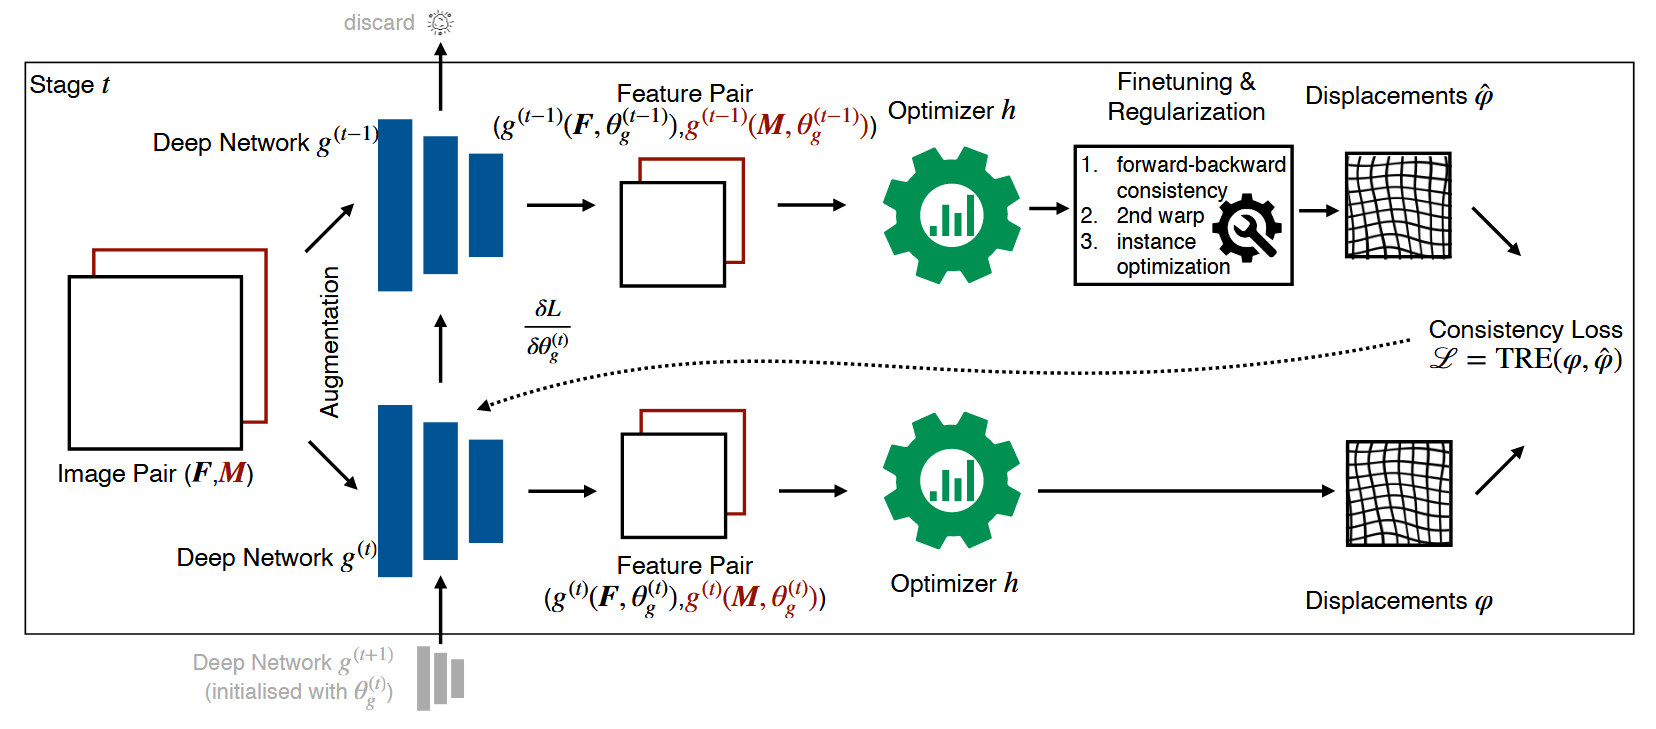
\includegraphics[width=0.9\textwidth]{T_RegCST.png}
  \bicaption[t-fig-c:1]{无监督注册的循环自训练范式概述}{底层配准流水线包括用于特征提取的深度网络g和用于预测位移的可微优化器h。在阶段t,我们使用基于前一阶段网络g(t-1)的特征生成的伪标签来监督网络g(t)的训练。对于最优特征学习,优化器的伪位移被进一步细化和正则化。}{Fig.$\!$ }{Overview of the proposed cyclical self-training paradigm for unsupervised registration. The underlying registration pipeline comprises a deep network for feature extraction g and a differentiable optimizer h to predict the displacements. At stage t, we supervise the training of the network $g^{(t)}$ with pseudo labels generated based on the features from the network $g^{(t-1)}$ from the previous stage. For optimal feature learning, the pseudo displacements from the optimizer are further refined and regularized.}
\end{figure}

\begin{equation}\tag*{(1)}
  f(\boldsymbol{F},\boldsymbol{M};\boldsymbol{\theta}_f)=h(g(\boldsymbol{F},\boldsymbol{M};\boldsymbol{\theta}_g))
\end{equation}

该方法基于我们的一项实证发现:即使使用随机初始化网络$g^{(0)}$(参数为$\theta_G^{(0)}$)提供的随机特征,合适的优化算法$h$仍能预测出合理的初始位移场$\hat{\boldsymbol{\varphi}}^{(0)}$,这与近期关于CNN归纳偏置的研究结论一致[4]。我们利用这些预测位移场作为伪标签来监督自训练的首阶段,通过最小化以下损失函数优化特征提取网络参数$\theta_G^{(1)}$:
\begin{equation}\tag*{(2)}
  \mathcal{L}(\boldsymbol{\theta}_g^{(1)};\mathcal{T})=\frac{1}{|\mathcal{T}|}\sum_i\mathrm{TRE}\left(h\left(g\left(\boldsymbol{F}_i,\boldsymbol{M}_i;\boldsymbol{\theta}_g^{(1)}\right)\right),\hat{\boldsymbol{\varphi}}_i^{(0)}\right)
\end{equation}
其中$\mathrm{TRE}(\hat{\boldsymbol{\varphi}}_\mathrm{i}^{(1)},\hat{\boldsymbol{\varphi}}_\mathrm{i}^{(0)})$表示位移场$\hat{\boldsymbol{\varphi}}_\mathrm{i}^{(1)}$与$\hat{\boldsymbol{\varphi}}_\mathrm{i}^{(0)}$逐元素目标配准误差的均值。

该基础框架存在网络可能过拟合初始伪标签并学习复制随机特征的关键问题。受对比学习最新技术启发[6],我们提出在学习和伪标签生成双路径中引入双重非对称性以增强特征学习效果:首先对双路径输入数据施加不同的随机增强;其次在伪标签路径的优化器后增加(不可微)细调与正则化步骤以提升伪位移场质量(详见第2.3节)。消融实验表明(图2、表1),这两种策略均可有效改善特征学习并强化自我增强效应。

当首阶段自训练收敛后,我们重复该过程$T$次迭代。具体而言,在第$t$阶段:1)使用前一阶段训练网络$g^{(t-1)}$生成精炼伪标签;2)以$g^{(t-1)}$权重初始化当前网络$g^{(t)}$;3)对学习率执行热重启以跳出前一阶段的局部极小值。

\subsection{配准框架}

我们提出的自训练方案是一个灵活、模块化的框架,其独立于输入模态及特征提取器$g$与优化器$h$的具体实现。本节阐述我们在图像和点云配准任务中对$g$和$h$的具体设计选择,其中图像配准为本文主要研究重点。

\textbf{图像配准.} 针对三维输入体数据,我们采用标准3D CNN实现特征提取器$g$。该网络包含六个卷积层,卷积核尺寸为3$\times$3$\times$3,通道数分别为32、64或128。每个卷积层后接批量归一化(BatchNorm)和ReLU激活函数,每隔一个卷积层进行步长为2的下采样,最终获得8倍降采样特征。通过1$\times$1$\times$1卷积将两幅图像特征映射至16维,并输入相关层[21]捕获125个离散位移。

作为优化器,我们基于文献[20]提出的耦合凸优化方法实现三维配准。该方法以固定和移动图像特征为输入,通过最小化平滑性与特征差异的联合目标函数推断位移场。伪标签流中的细化策略包含三个关键要素:1) 前向-后向一致性:额外计算反向位移场($\boldsymbol{F}$到$\boldsymbol{M}$),并通过迭代优化最小化双向场间差异;2) 二次形变:使用当前位移场对移动图像进行形变后重复前述步骤;3) 迭代实例优化:采用Adam算法联合最小化正则化代价与特征差异,对最终位移场进行微调。其中特征差异计算使用第二卷积块后的CNN特征(经1$\times$1$\times$1卷积映射至16通道)。在测试阶段采用相同的细化步骤。

此外,我们提出通过比较网络预测位移与微调后位移的差异来估计训练样本难度。据此实施加权批量采样策略,优先选择场间一致性更高的简单配准对。具体实现中,对所有训练对进行难度排序,并采用参数范围-5至5的sigmoid函数构建加权随机采样器。

\textbf{点云配准.} 对于点云配准任务,我们采用图卷积网络实现特征提取器,并基于文献[9]提出的可微分稀疏循环置信传播算法进行优化。

\section{实验}

\subsection{实验设置}

\textbf{数据集.} 我们在Learn2Reg (L2R)挑战赛[15]的跨患者腹部CT配准数据集上进行主要实验。该数据集包含30例不同患者的三维腹部CT扫描数据,包含13个尺寸差异显著的手动标注解剖结构。原始影像数据与标签来源于[26]。作为L2R基准的一部分,数据经仿射预配准至标准空间,并重采样为统一体素分辨率(2毫米)和空间维度(192$\times$160$\times$256体素)。遵循L2R数据划分方案,使用20例扫描(190对)进行训练,剩余10例(45对)用于评估。数据划分与预处理流程与对比方法[9,27]保持一致。评估指标采用语义标签间的平均Dice相似系数(DSC)及对数雅可比行列式标准差(SDlogJ)。

我们使用DIR-Lab COPDGene数据集[5]进行呼气-吸气相位肺部CT配准的补充实验,该数据集包含10组扫描对。每组扫描提供300个专家标注的解剖标志点用于评估。预处理流程包含:1) 呼气相扫描重采样至1.75$\times$1.00$\times$1.25毫米,吸气相至1.75$\times$1.25$\times$1.75毫米;2) 基于自动生成肺部分割掩膜,截取固定尺寸感兴趣区域(192$\times$192$\times$208体素);3) 对肺部分割结果进行仿射预配准。针对肺部CT关键点配准任务,我们遵循[9]的方法,使用Förstner算法结合非极大值抑制提取CT影像特征点,固定影像约生成1,000个点,移动影像约2,000个点。实验采用五折交叉验证,每折包含8对训练数据和2对测试数据。评估指标为标志点处目标配准误差(TRE)及SDlogJ。

\textbf{实现细节.} 所有方法基于PyTorch框架实现,使用Adam优化器进行网络参数优化。腹部配准任务设置$T$=8个训练阶段,每阶段包含1,000次迭代(batch size=2),学习率采用余弦退火热重启策略,每阶段从$10^{-3}$衰减至$10^{-5}$。超参数根据训练集三个病例的DSC指标确定。肺部配准任务经过$T$=5个阶段(每阶段60个epoch,batch size=4)达到收敛,初始学习率0.001,分别在第40和52 epoch衰减10倍。该任务超参数继承自[9]。两个数据集训练过程均在RTX2080显卡(8GB显存)上完成,耗时约90-100分钟,数据增强采用随机仿射变换。

\subsection{结果}

\textbf{腹部实验.} 首先通过消融实验分析本方法性能。图2展示了多个自训练周期中不同解剖结构类别的配准效果演变,可见各阶段性能持续提升(尤其在早期阶段显著),最终趋于收敛。这验证了伪标签更新与网络训练交替机制产生的自我增强效应。表1上半部分验证了双路径非对称增强(输入增强、伪标签微调)及加权采样策略的有效性,结果表明各组件对实现最优性能均具有重要作用。表1下半部分评估了不同测试配置下的模型表现,结果显示二次形变与Adam微调可带来显著性能提升。

\begin{figure}
  \centering
  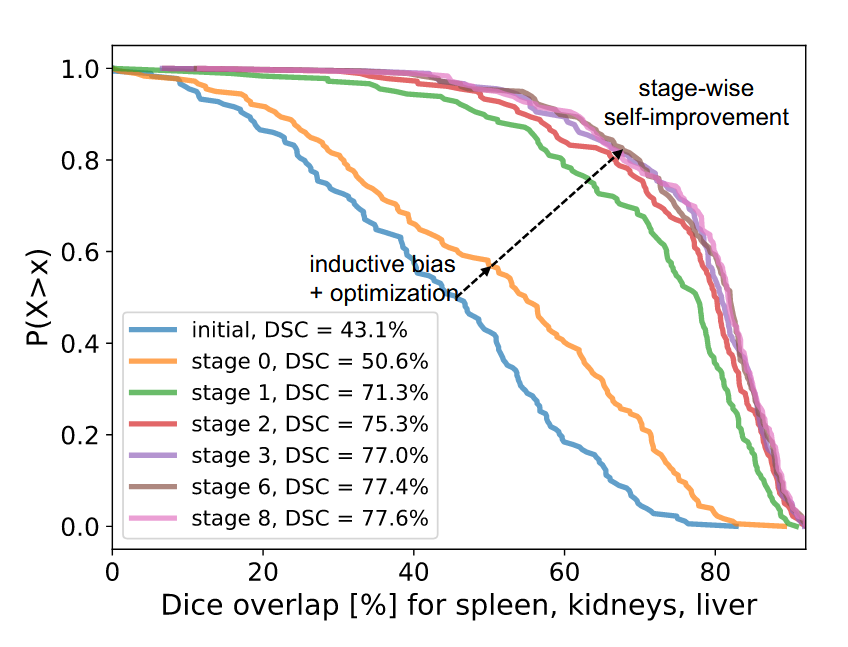
\includegraphics[width=0.9\textwidth]{T_result.png}
  \bicaption[t-fig-c:2]{}{在不同阶段的自我训练后,腹部CT登记的Dice重叠的“相反”累积分布。}{Fig.$\!$ }{“Opposite” cumulative distribution of Dice overlaps for Abdomen CT registration after different stages of self-training.}
\end{figure}

\begin{table}
  \bicaption[t-c:table1]{}{腹部CT配准的消融研究。}{Table$\!$}{Ablation study for abdomen CT registration.}
  \vspace{0.5em}\centering\wuhao
  \begin{tabular}{lcc}
    \toprule
    \textbf{Method}       & \textbf{DSC}  & \textbf{SDlogJ} \\
    \midrule
    prealign              & 25.9          & --              \\
    w/o input augm.       & 48.8          & 0.129           \\
    w/o PL refinement     & 48.8          & 0.200           \\
    w/o weighted sampling & 50.1          & 0.147           \\
    ours                  & 51.1          & 0.146           \\
    \midrule
    1 warp w/o Adam       & 38.6          & 0.061           \\
    1 warp w/ Adam        & 49.6          & 0.119           \\
    2 warps w/o Adam      & 41.1          & 0.088           \\
    2 warps w/Adam (ours) & \textbf{51.1} & 0.146           \\
    \bottomrule
  \end{tabular}
\end{table}

随后,我们将本方法与包括经典算法[1,10,14]和深度学习方法在内的多种最先进无监督方法进行对比,其中深度学习方法涵盖MIND[2,12]/NCC[17]监督训练和对比学习[27]方案。对比数据引自文献[9]与[27]。为直接验证自训练策略优势,我们还使用基于度量的监督方法(MIND[13]、NCC[19])训练了相同框架。实验结果见表2、图3及补充材料图3。本方法在DSC指标上显著超越所有对比方法(对公开代码方法进行Wilcoxon符号秩检验,p<0.0001;SAME方法因未公开代码未参与检验),以51.1\%的DSC刷新当前最佳性能。这证明了新学习范式相较于传统无监督策略的优越性。同时,预测位移场的平滑性指标(SDlogJ)与多数无监督深度方法[2,12]相当,且优于MIND与NCC监督方法。

\begin{figure}
  \centering
  \includegraphics[width=0.9\textwidth]{T_img.png}
  \bicaption[ct-fig:3]{}{所选方法对两例腹部CT数据集(轴向视图)的定性结果。我们展示了扭曲分割标签与固定扫描的叠加}{Fig.$\!$ }{Qualitative results of selected methods on two cases of the Abdomen CT dataset (axial view). We show overlays of the warped segmentation labels with the fixed scan.}
\end{figure}

\begin{table}
  \bicaption[ct:table2]{}{无监督腹部CT配准结果}{Table$\!$}{Results for unsupervised abdomen CT registration.}
  \vspace{0.5em}\centering\wuhao
  \begin{tabular}{lccc}
    \toprule
    \textbf{Method} & \textbf{Dice [\%]} & \textbf{SDlogJ} & \textbf{Time [s]} \\
    \midrule
    pre-aligned     & 25.9               & --              & --                \\
    Adam            & 36.6               & 0.080           & 1.6               \\
    Iter. LBP       & 40.1               & 0.093           & 0.6               \\
    ANTs (SyN)      & 28.4               & {N/A}           & 74.3              \\
    DEEDS           & 46.5               & {N/A}           & 45.4              \\
    \midrule
    VoxelMorph      & 35.4               & 0.134           & 0.2               \\
    PDD             & 41.5               & 0.129           & 1.4               \\
    LapIRN          & 42.4               & 0.089           & 3.8               \\
    SAME            & 49.8               & {N/A}           & 1.2               \\
    \midrule
    MIND sup.       & 47.7               & 0.237           & 1.2               \\
    NCC sup.        & 48.1               & 0.299           & 1.2               \\
    \midrule
    ours            & \textbf{51.1}      & 0.146           & 1.2               \\
    \bottomrule
  \end{tabular}
\end{table}

\textbf{肺部实验.} 在基于点云的肺部配准任务中,我们将循环自训练策略与三种学习方案进行对比:1) 基于人工标注标志点的监督学习[9];2) 结合倒角距离与局部拉普拉斯惩罚的度量监督[23];3) 合成刚性/随机形变场训练。所有策略均基于文献[9]的基准模型实现。此外,我们还对比了三种基于MIND监督的无监督图像配准方法[2,12,17]。表3结果显示,本自训练策略在所有对比方案及现有图像配准SOTA方法中均表现出最优性能。补充材料图4展示了实验的定性结果,可见预测位移场兼具高精度与平滑性,该结论亦得到低SDlogJ值的支持。

\section{结论}

我们提出了一种新型的循环自训练范式用于无监督配准任务。为此,我们开发了模块化的配准流程框架,该框架将深度特征提取网络与可微分优化器相结合,通过正则化与迭代式循环精炼机制,有效稳定了噪声伪标签下的学习过程。相较于依赖浅层特征或图像强度的传统度量监督方法(如NCC、MIND)——这类方法易受噪声干扰并陷入局部极小——我们的优化驱动伪标签监督机制具有显著优势:1)基于优化精炼与正则化的伪标签能够引导网络学习更具噪声鲁棒性的任务相关特征;2)循环学习策略通过渐进式特征增强有效避免局部极小。实验结果表明,本方法在密集图像腹部配准与点云肺部配准任务中均超越当前最先进方法,充分验证了方案的有效性与灵活性。综上所述,本研究不仅首次实现了完全无监督的自训练框架,更为基于学习的无监督配准提供了全新视角。特别值得指出的是,本策略与现有技术(度量监督与对比学习)具有互补性,为未来构建联合训练方案开辟了新可能。

% \title{The title of the English paper}

% \textbf{Abstract:} As one of the most widely used techniques in operations
% research, \emph{ mathematical programming} is defined as a means of maximizing a
% quantity known as \emph{bjective function}, subject to a set of constraints
% represented by equations and inequalities. Some known subtopics of mathematical
% programming are linear programming, nonlinear programming, multiobjective
% programming, goal programming, dynamic programming, and multilevel
% programming$^{[1]}$.

% It is impossible to cover in a single chapter every concept of mathematical
% programming. This chapter introduces only the basic concepts and techniques of
% mathematical programming such that readers gain an understanding of them
% throughout the book$^{[2,3]}$.


% \section{Single-Objective Programming}
% The general form of single-objective programming (SOP) is written
% as follows,
% \begin{equation}\tag*{(123)} % 如果附录中的公式不想让它出现在公式索引中,那就请
%                              % 用 \tag*{xxxx}
% \left\{\begin{array}{l}
% \max \,\,f(x)\\[0.1 cm]
% \mbox{subject to:} \\ [0.1 cm]
% \qquad g_j(x)\le 0,\quad j=1,2,\cdots,p
% \end{array}\right.
% \end{equation}
% which maximizes a real-valued function $f$ of
% $x=(x_1,x_2,\cdots,x_n)$ subject to a set of constraints.

% \newtheorem{mpdef}{Definition}[chapter]
% \begin{mpdef}
% In SOP, we call $x$ a decision vector, and
% $x_1,x_2,\cdots,x_n$ decision variables. The function
% $f$ is called the objective function. The set
% \begin{equation}\tag*{(456)} % 这里同理,其它不再一一指定。
% S=\left\{x\in\Re^n\bigm|g_j(x)\le 0,\,j=1,2,\cdots,p\right\}
% \end{equation}
% is called the feasible set. An element $x$ in $S$ is called a
% feasible solution.
% \end{mpdef}

% \newtheorem{mpdefop}[mpdef]{Definition}
% \begin{mpdefop}
% A feasible solution $x^*$ is called the optimal
% solution of SOP if and only if
% \begin{equation}
% f(x^*)\ge f(x)
% \end{equation}
% for any feasible solution $x$.
% \end{mpdefop}

% One of the outstanding contributions to mathematical programming was known as
% the Kuhn-Tucker conditions\ref{eq:ktc}. In order to introduce them, let us give
% some definitions. An inequality constraint $g_j(x)\le 0$ is said to be active at
% a point $x^*$ if $g_j(x^*)=0$. A point $x^*$ satisfying $g_j(x^*)\le 0$ is said
% to be regular if the gradient vectors $\nabla g_j(x)$ of all active constraints
% are linearly independent.

% Let $x^*$ be a regular point of the constraints of SOP and assume that all the
% functions $f(x)$ and $g_j(x),j=1,2,\cdots,p$ are differentiable. If $x^*$ is a
% local optimal solution, then there exist Lagrange multipliers
% $\lambda_j,j=1,2,\cdots,p$ such that the following Kuhn-Tucker conditions hold,
% \begin{equation}
% \label{eq:ktc}
% \left\{\begin{array}{l}
%     \nabla f(x^*)-\sum\limits_{j=1}^p\lambda_j\nabla g_j(x^*)=0\\[0.3cm]
%     \lambda_jg_j(x^*)=0,\quad j=1,2,\cdots,p\\[0.2cm]
%     \lambda_j\ge 0,\quad j=1,2,\cdots,p.
% \end{array}\right.
% \end{equation}
% If all the functions $f(x)$ and $g_j(x),j=1,2,\cdots,p$ are convex and
% differentiable, and the point $x^*$ satisfies the Kuhn-Tucker conditions
% (\ref{eq:ktc}), then it has been proved that the point $x^*$ is a global optimal
% solution of SOP.

% \subsection{Linear Programming}
% \label{sec:lp}

% If the functions $f(x),g_j(x),j=1,2,\cdots,p$ are all linear, then SOP is called
% a {\em linear programming}.

% The feasible set of linear is always convex. A point $x$ is called an extreme
% point of convex set $S$ if $x\in S$ and $x$ cannot be expressed as a convex
% combination of two points in $S$. It has been shown that the optimal solution to
% linear programming corresponds to an extreme point of its feasible set provided
% that the feasible set $S$ is bounded. This fact is the basis of the {\em simplex
%   algorithm} which was developed by Dantzig as a very efficient method for
% solving linear programming.
% \begin{table}[ht]
% \centering
%   \centering
%   \caption*{Table~1\hskip1em This is an example for manually numbered table, which
%     would not appear in the list of tables}
%   \label{tab:badtabular2}
%   \begin{tabular}[c]{|m{1.5cm}|c|c|c|c|c|c|}\hline
%     \multicolumn{2}{|c|}{Network Topology} & \# of nodes &
%     \multicolumn{3}{c|}{\# of clients} & Server \\\hline
%     GT-ITM & Waxman Transit-Stub & 600 &
%     \multirow{2}{2em}{2\%}&
%     \multirow{2}{2em}{10\%}&
%     \multirow{2}{2em}{50\%}&
%     \multirow{2}{1.2in}{Max. Connectivity}\\\cline{1-3}
%     \multicolumn{2}{|c|}{Inet-2.1} & 6000 & & & &\\\hline
%     & \multicolumn{2}{c|}{ABCDEF} &\multicolumn{4}{c|}{} \\\hline
% \end{tabular}
% \end{table}

% Roughly speaking, the simplex algorithm examines only the extreme points of the
% feasible set, rather than all feasible points. At first, the simplex algorithm
% selects an extreme point as the initial point. The successive extreme point is
% selected so as to improve the objective function value. The procedure is
% repeated until no improvement in objective function value can be made. The last
% extreme point is the optimal solution.

% \subsection{Nonlinear Programming}

% If at least one of the functions $f(x),g_j(x),j=1,2,\cdots,p$ is nonlinear, then
% SOP is called a {\em nonlinear programming}.

% A large number of classical optimization methods have been developed to treat
% special-structural nonlinear programming based on the mathematical theory
% concerned with analyzing the structure of problems.

% Now we consider a nonlinear programming which is confronted solely with
% maximizing a real-valued function with domain $\Re^n$.  Whether derivatives are
% available or not, the usual strategy is first to select a point in $\Re^n$ which
% is thought to be the most likely place where the maximum exists. If there is no
% information available on which to base such a selection, a point is chosen at
% random. From this first point an attempt is made to construct a sequence of
% points, each of which yields an improved objective function value over its
% predecessor. The next point to be added to the sequence is chosen by analyzing
% the behavior of the function at the previous points. This construction continues
% until some termination criterion is met. Methods based upon this strategy are
% called {\em ascent methods}, which can be classified as {\em direct methods},
% {\em gradient methods}, and {\em Hessian methods} according to the information
% about the behavior of objective function $f$. Direct methods require only that
% the function can be evaluated at each point. Gradient methods require the
% evaluation of first derivatives of $f$. Hessian methods require the evaluation
% of second derivatives. In fact, there is no superior method for all
% problems. The efficiency of a method is very much dependent upon the objective
% function.

% \subsection{Integer Programming}

% {\em Integer programming} is a special mathematical programming in which all of
% the variables are assumed to be only integer values. When there are not only
% integer variables but also conventional continuous variables, we call it {\em
%   mixed integer programming}. If all the variables are assumed either 0 or 1,
% then the problem is termed a {\em zero-one programming}. Although integer
% programming can be solved by an {\em exhaustive enumeration} theoretically, it
% is impractical to solve realistically sized integer programming problems. The
% most successful algorithm so far found to solve integer programming is called
% the {\em branch-and-bound enumeration} developed by Balas (1965) and Dakin
% (1965). The other technique to integer programming is the {\em cutting plane
%   method} developed by Gomory (1959).

% \hfill\textit{Uncertain Programming\/}\quad(\textsl{BaoDing Liu, 2006.2})

% \section*{References}
% \noindent{\itshape NOTE: These references are only for demonstration. They are
%   not real citations in the original text.}

% \begin{translationbib}
% \item Donald E. Knuth. The \TeX book. Addison-Wesley, 1984. ISBN: 0-201-13448-9
% \item Paul W. Abrahams, Karl Berry and Kathryn A. Hargreaves. \TeX\ for the
%   Impatient. Addison-Wesley, 1990. ISBN: 0-201-51375-7
% \item David Salomon. The advanced \TeX book.  New York : Springer, 1995. ISBN:0-387-94556-3
% \end{translationbib}

% \chapter{外文资料的调研阅读报告或书面翻译}

% \title{英文资料的中文标题}

% {\heiti 摘要:} 本章为外文资料翻译内容。如果有摘要可以直接写上来,这部分好像没有
% 明确的规定。

% \section{单目标规划}
% 北冥有鱼,其名为鲲。鲲之大,不知其几千里也。化而为鸟,其名为鹏。鹏之背,不知其几
% 千里也。怒而飞,其翼若垂天之云。是鸟也,海运则将徙于南冥。南冥者,天池也。
% \begin{equation}\tag*{(123)}
%  p(y|\mathbf{x}) = \frac{p(\mathbf{x},y)}{p(\mathbf{x})}=
% \frac{p(\mathbf{x}|y)p(y)}{p(\mathbf{x})}
% \end{equation}

% 吾生也有涯,而知也无涯。以有涯随无涯,殆已!已而为知者,殆而已矣!为善无近名,为
% 恶无近刑,缘督以为经,可以保身,可以全生,可以养亲,可以尽年。

% \subsection{线性规划}
% 庖丁为文惠君解牛,手之所触,肩之所倚,足之所履,膝之所倚,砉然响然,奏刀騞然,莫
% 不中音,合于桑林之舞,乃中经首之会。
% \begin{table}[ht]
% \centering
%   \centering
%   \caption*{表~1\hskip1em 这是手动编号但不出现在索引中的一个表格例子}
%   \label{tab:badtabular3}
%   \begin{tabular}[c]{|m{1.5cm}|c|c|c|c|c|c|}\hline
%     \multicolumn{2}{|c|}{Network Topology} & \# of nodes &
%     \multicolumn{3}{c|}{\# of clients} & Server \\\hline
%     GT-ITM & Waxman Transit-Stub & 600 &
%     \multirow{2}{2em}{2\%}&
%     \multirow{2}{2em}{10\%}&
%     \multirow{2}{2em}{50\%}&
%     \multirow{2}{1.2in}{Max. Connectivity}\\\cline{1-3}
%     \multicolumn{2}{|c|}{Inet-2.1} & 6000 & & & &\\\hline
%     & \multicolumn{2}{c|}{ABCDEF} &\multicolumn{4}{c|}{} \\\hline
% \end{tabular}
% \end{table}

% 文惠君曰:“嘻,善哉!技盖至此乎?”庖丁释刀对曰:“臣之所好者道也,进乎技矣。始臣之
% 解牛之时,所见无非全牛者;三年之后,未尝见全牛也;方今之时,臣以神遇而不以目视,
% 官知止而神欲行。依乎天理,批大郤,导大窾,因其固然。技经肯綮之未尝,而况大坬乎!
% 良庖岁更刀,割也;族庖月更刀,折也;今臣之刀十九年矣,所解数千牛矣,而刀刃若新发
% 于硎。彼节者有间而刀刃者无厚,以无厚入有间,恢恢乎其于游刃必有余地矣。是以十九年
% 而刀刃若新发于硎。虽然,每至于族,吾见其难为,怵然为戒,视为止,行为迟,动刀甚微,
% 謋然已解,如土委地。提刀而立,为之而四顾,为之踌躇满志,善刀而藏之。”

% 文惠君曰:“善哉!吾闻庖丁之言,得养生焉。”


% \subsection{非线性规划}
% 孔子与柳下季为友,柳下季之弟名曰盗跖。盗跖从卒九千人,横行天下,侵暴诸侯。穴室枢
% 户,驱人牛马,取人妇女。贪得忘亲,不顾父母兄弟,不祭先祖。所过之邑,大国守城,小
% 国入保,万民苦之。孔子谓柳下季曰:“夫为人父者,必能诏其子;为人兄者,必能教其弟。
% 若父不能诏其子,兄不能教其弟,则无贵父子兄弟之亲矣。今先生,世之才士也,弟为盗
% 跖,为天下害,而弗能教也,丘窃为先生羞之。丘请为先生往说之。”

% 柳下季曰:“先生言为人父者必能诏其子,为人兄者必能教其弟,若子不听父之诏,弟不受
% 兄之教,虽今先生之辩,将奈之何哉?且跖之为人也,心如涌泉,意如飘风,强足以距敌,
% 辩足以饰非。顺其心则喜,逆其心则怒,易辱人以言。先生必无往。”

% 孔子不听,颜回为驭,子贡为右,往见盗跖。

% \subsection{整数规划}
% 盗跖乃方休卒徒大山之阳,脍人肝而餔之。孔子下车而前,见谒者曰:“鲁人孔丘,闻将军
% 高义,敬再拜谒者。”谒者入通。盗跖闻之大怒,目如明星,发上指冠,曰:“此夫鲁国之
% 巧伪人孔丘非邪?为我告之:尔作言造语,妄称文、武,冠枝木之冠,带死牛之胁,多辞缪
% 说,不耕而食,不织而衣,摇唇鼓舌,擅生是非,以迷天下之主,使天下学士不反其本,妄
% 作孝弟,而侥幸于封侯富贵者也。子之罪大极重,疾走归!不然,我将以子肝益昼餔之膳。”


% \chapter{其它附录}
% 前面两个附录主要是给本科生做例子。其它附录的内容可以放到这里,当然如果你愿意,可
% 以把这部分也放到独立的文件中,然后将其到主文件中。
%本科生翻译论文
% \end{appendix}
%%%%%%%%%%%%%%%%%%%%%%%%%%%%%%%%%%%%%%%%%%%%%%%%%%%%%%%%%%%%%%%%%%%%%%%%%%%%%%%%
% 硕博书序
%%%%%%%%%%%%%%%%%%%%%%%%%%%%%%%%%%%%%%%%%%%%%%%%%%%%%%%%%%%%%%%%%%%%%%%%%%%%%%%%
% \bibliography{reference} % 参考文献
% \begin{appendix}%附录
% \input{back/appA.tex}
% \end{appendix}
% \include{back/publications}    % 所发文章
% \include{back/ceindex}    % 索引, 根据自己的情况添加或者不添加,选择自动添加或者手工添加。
% \authorization %授权
% %\authorization[scan.pdf] %添加扫描页的命令,与上互斥
% % !Mode:: "TeX:UTF-8"
\begin{acknowledgements}

在我完成本论文之际,心中感慨万千,衷心感谢在这段旅程中给予我支持与帮助的人们。首先,我要特别感谢我的指导老师骆功宁教授。您以渊博的知识和严谨的治学态度,给予我悉心的指导和耐心的教诲。在整个毕设过程中,您不仅为我指明了研究的方向,更以您的严谨与热情感染了我,让我在困惑与迷茫中找到了前进的动力。每一次的讨论与交流,都让我豁然开朗,能够顺利完成论文,离不开您的辛勤付出。

同时,我也要感谢我的同学们。在这段重要的时光里,大家的支持与帮助让我倍感温暖。在无数个深夜的图书馆学习时光中,我们相互鼓励,分享经验,共同克服各种困难。无论是对论文的讨论,还是对生活的倾诉,都是我大学生活中的美好瞬间。你们的陪伴,让我在求学路上不再孤单,成为我最宝贵的财富。

此外,我非常感谢我的家人。你们无条件的支持与理解,是我在追求学术道路上最大的动力。在我遇到困难时,你们给予我温暖的鼓励,始终相信我、支持我,帮助我渡过一个又一个难关。感恩有你们的陪伴,才让我拥有了克服挑战的勇气与信心。

我也要感谢验收时各位老师对我论文格式和内容的指导,您们的专业意见与建议使我的论文更加完善。每一位老师的认真审阅和点评都让我获益匪浅,您的严谨与负责让我明白了学术研究的严肃性,也让我学会了在不断修正中追求卓越。

历历浮生,无非败而后成。回首大学四年,我经历了学习的高峰与低谷,收获了知识与友谊,更锻炼了自己的意志与品格。每一个坚持的时刻都在教会我,持之以恒的努力终会迎来丰硕的成果。感谢我自己在这条道路上的坚持与努力,没有放弃,是我走到今天的重要原因。未来的路依然漫长,我会带着这份感恩与勇气,继续前行。

衷心感谢每一位在我人生旅程中给予我帮助的人,愿我们都能在各自的领域中,不断追求卓越,共同成就美好的未来。


\end{acknowledgements}
 %致谢
% \include{back/resume}          % 博士学位论文有个人简介
%%%%%%%%%%%%%%%%%%%%%%%%%%%%%%%%%%%%%%%%%%%%%%%%%%%%%%%%%%%%%%%%%%%%%%%%%%%%%%%%
% 博后书序
%%%%%%%%%%%%%%%%%%%%%%%%%%%%%%%%%%%%%%%%%%%%%%%%%%%%%%%%%%%%%%%%%%%%%%%%%%%%%%%%
% \bibliography{reference} % 参考文献
% % !Mode:: "TeX:UTF-8"
\begin{acknowledgements}

在我完成本论文之际,心中感慨万千,衷心感谢在这段旅程中给予我支持与帮助的人们。首先,我要特别感谢我的指导老师骆功宁教授。您以渊博的知识和严谨的治学态度,给予我悉心的指导和耐心的教诲。在整个毕设过程中,您不仅为我指明了研究的方向,更以您的严谨与热情感染了我,让我在困惑与迷茫中找到了前进的动力。每一次的讨论与交流,都让我豁然开朗,能够顺利完成论文,离不开您的辛勤付出。

同时,我也要感谢我的同学们。在这段重要的时光里,大家的支持与帮助让我倍感温暖。在无数个深夜的图书馆学习时光中,我们相互鼓励,分享经验,共同克服各种困难。无论是对论文的讨论,还是对生活的倾诉,都是我大学生活中的美好瞬间。你们的陪伴,让我在求学路上不再孤单,成为我最宝贵的财富。

此外,我非常感谢我的家人。你们无条件的支持与理解,是我在追求学术道路上最大的动力。在我遇到困难时,你们给予我温暖的鼓励,始终相信我、支持我,帮助我渡过一个又一个难关。感恩有你们的陪伴,才让我拥有了克服挑战的勇气与信心。

我也要感谢验收时各位老师对我论文格式和内容的指导,您们的专业意见与建议使我的论文更加完善。每一位老师的认真审阅和点评都让我获益匪浅,您的严谨与负责让我明白了学术研究的严肃性,也让我学会了在不断修正中追求卓越。

历历浮生,无非败而后成。回首大学四年,我经历了学习的高峰与低谷,收获了知识与友谊,更锻炼了自己的意志与品格。每一个坚持的时刻都在教会我,持之以恒的努力终会迎来丰硕的成果。感谢我自己在这条道路上的坚持与努力,没有放弃,是我走到今天的重要原因。未来的路依然漫长,我会带着这份感恩与勇气,继续前行。

衷心感谢每一位在我人生旅程中给予我帮助的人,愿我们都能在各自的领域中,不断追求卓越,共同成就美好的未来。


\end{acknowledgements}
 %致谢
% \include{back/doctorpublications}    % 所发文章
% \include{back/publications}    % 所发文章
% \include{back/resume}          % 博士学位论文有个人简介
% \include{back/correspondingaddr} %通信地址
%%%%%%%%%%%%%%%%%%%%%%%%%%%%%%%%%%%%%%%%%%%%%%%%%%%%%%%%%%%%%%%%%%%%%%%%%%%%%%%%
\end{document}
% Local Variables:
% TeX-engine: xetex
% End:
